%============================================================================%
% Antoine Gé́ré (gereantoine@gmail.com).
%============================================================================%


% LaTeX environment used : Kile, available at : http://kile.sourceforge.net/
%
% Package used : available at http://www.ctan.org/
%
% The comprehensive latex symbole list : available at http://www.ctan.org/tex-archive/info/symbols/comprehensive/
% and Detexif, an attempt to simplify to search in the list : available at http://detexify.kirelabs.org/classify.html
%
% Bibliography done with Zotero, available at : https://www.zotero.org/
% Bibtex style ????? .


%----------------------------------------------------------------------------%

\documentclass[10pt]{book}

%----------------------------------------------------------------------------%

%a
\usepackage{amscd}
\usepackage{amsmath}
\usepackage{amsfonts}
\usepackage{amssymb}
\usepackage{amsxtra}
\usepackage{array} 
%b
\usepackage[english]{babel}
%c
\usepackage{calligra}
\usepackage{cite}
\usepackage{color}
%e
\usepackage{enumitem}
%f
\usepackage{fancyhdr}
\usepackage{filecontents}
\usepackage[T1]{fontenc}
%g
\usepackage{geometry}
%h
\usepackage{hyperref}
%i
\usepackage[totoc]{idxlayout}
\usepackage[utf8]{inputenc}
%m
\usepackage{makeidx}
%n
\usepackage[amsmath,amsthm,thmmarks]{ntheorem}
%p
\usepackage{palatino}
%q
\usepackage[sfdefault]{quattrocento}
%t
\usepackage{tikz}
%u
\usepackage{upgreek}
%w
\usepackage{wrapfig}

%----------------------------------------------------------------------------%

%\begin{filecontents}{biblio.bib}
%
%
%
%
%\end{filecontents}

%----------------------------------------------------------------------------%

\geometry{
a4paper,
left=20mm,
right=20mm,
top=20mm,
bottom=20mm,
}

%----------------------------------------------------------------------------%

\setlength\parindent{0pt}

%----------------------------------------------------------------------------%

\pdfoptionpdfminorversion=6

%----------------------------------------------------------------------------%

\makeindex

%----------------------------------------------------------------------------%

\renewcommand{\headrulewidth}{0pt}
\renewcommand{\footrulewidth}{0pt}

\setlength{\headheight}{22pt} 

\pagestyle{fancy}
%
\renewcommand{\chaptermark}[1]{ \markboth{#1}{} }
\renewcommand{\sectionmark}[1]{ \markright{#1} }
%
\fancyhf{}
\fancyhead[LE,RO]{\thepage}
\fancyhead[RE,CE]{}
\fancyhead[LO,CO]{}

\fancypagestyle{plain}{ %
\fancyhf{}
}

\DeclareMathAlphabet{\mathcalligra}{T1}{calligra}{m}{n}

%----------------------------------------------------------------------------%

\newcommand{\supp}{\mathsf{supp}}
\newcommand{\WF}{\mathsf{WF}}
\newcommand{\id}{\mathsf{id}}
\newcommand{\loc}{\mathsf{loc}}
\newcommand{\reg}{\mathsf{reg}}
\newcommand{\pp}{\mathsf{pp}}
\newcommand{\ms}{\mathsf{ms}}
\newcommand{\sd}{\mathsf{sd}}
\newcommand{\vol}{\mathsf{vol}}
\newcommand{\tr}{\mathsf{tr}}

\newcommand{\abs}[1]{\left|#1\right|}
\newcommand{\norm}[1]{\left|\left|#1\right|\right|}
\newcommand{\sm}[1]{\left\langle#1\right\rangle}
\newcommand{\wick}[1]{:\!{#1}\!:}

\renewcommand{\det}{\mathsf{det}}
\renewcommand{\sup}{\mathsf{sup}}
\renewcommand{\inf}{\mathsf{inf}}

\let\int\int
\def\bigint{\displaystyle\int}

%----------------------------------------------------------------------------%

\newcommand{\Acal}{\mathcal{A}}
\newcommand{\Bcal}{\mathcal{B}}
\newcommand{\Ccal}{\mathcal{C}}
\newcommand{\Dcal}{\mathcal{D}}
\newcommand{\Ecal}{\mathcal{E}}
\newcommand{\Fcal}{\mathcal{F}}
\newcommand{\Gcal}{\mathcal{G}}
\newcommand{\Hcal}{\mathcal{H}}
\newcommand{\Ical}{\mathcal{I}}
\newcommand{\Jcal}{\mathcal{J}}
\newcommand{\Kcal}{\mathcal{K}}
\newcommand{\Lcal}{\mathcal{L}}
\newcommand{\Mcal}{\mathcal{M}}
\newcommand{\Ncal}{\mathcal{N}}
\newcommand{\Ocal}{\mathcal{O}}
\newcommand{\Pcal}{\mathcal{P}}
\newcommand{\Qcal}{\mathcal{Q}}
\newcommand{\Rcal}{\mathcal{R}}
\newcommand{\Scal}{\mathcal{S}}
\newcommand{\Tcal}{\mathcal{T}}
\newcommand{\Ucal}{\mathcal{U}}
\newcommand{\Vcal}{\mathcal{V}}
\newcommand{\Wcal}{\mathcal{W}}
\newcommand{\Xcal}{\mathcal{X}}
\newcommand{\Ycal}{\mathcal{Y}}
\newcommand{\Zcal}{\mathcal{Z}}

%----------------------------------------------------------------------------%

\newcommand{\Abb}{\mathbb{A}}
\newcommand{\Bmbb}{\mathbb{B}}
\newcommand{\Cbb}{\mathbb{C}}
\newcommand{\Dbb}{\mathbb{D}}
\newcommand{\Ebb}{\mathbb{E}}
\newcommand{\Fbb}{\mathbb{F}}
\newcommand{\Gbb}{\mathbb{G}}
\newcommand{\Hbb}{\mathbb{H}}
\newcommand{\Ibb}{\mathbb{I}}
\newcommand{\Jbb}{\mathbb{J}}
\newcommand{\Kbb}{\mathbb{K}}
\newcommand{\Lbb}{\mathbb{L}}
\newcommand{\Mbb}{\mathbb{M}}
\newcommand{\Nbb}{\mathbb{N}}
\newcommand{\Obb}{\mathbb{O}}
\newcommand{\Pbb}{\mathbb{P}}
\newcommand{\Qbb}{\mathbb{Q}}
\newcommand{\Rbb}{\mathbb{R}}
\newcommand{\Sbb}{\mathbb{S}}
\newcommand{\Tbb}{\mathbb{T}}
\newcommand{\Ubb}{\mathbb{U}}
\newcommand{\Vbb}{\mathbb{V}}
\newcommand{\Wbb}{\mathbb{W}}
\newcommand{\Xbb}{\mathbb{X}}
\newcommand{\Ybb}{\mathbb{Y}}
\newcommand{\Zbb}{\mathbb{Z}}

%----------------------------------------------------------------------------%

\newcommand{\Arak}{\mathfrak{A}}
\newcommand{\Brak}{\mathfrak{B}}
\newcommand{\Crak}{\mathfrak{C}}
\newcommand{\Drak}{\mathfrak{D}}
\newcommand{\Erak}{\mathfrak{E}}
\newcommand{\Frak}{\mathfrak{F}}
\newcommand{\Grak}{\mathfrak{G}}
\newcommand{\Hrak}{\mathfrak{H}}
\newcommand{\Irak}{\mathfrak{I}}
\newcommand{\Jrak}{\mathfrak{J}}
\newcommand{\Krak}{\mathfrak{K}}
\newcommand{\Lrak}{\mathfrak{L}}
\newcommand{\Mrak}{\mathfrak{M}}
\newcommand{\Nrak}{\mathfrak{N}}
\newcommand{\Orak}{\mathfrak{O}}
\newcommand{\Prak}{\mathfrak{P}}
\newcommand{\Qrak}{\mathfrak{Q}}
\newcommand{\Rrak}{\mathfrak{R}}
\newcommand{\Srak}{\mathfrak{S}}
\newcommand{\Trak}{\mathfrak{T}}
\newcommand{\Urak}{\mathfrak{U}}
\newcommand{\Vrak}{\mathfrak{V}}
\newcommand{\Wrak}{\mathfrak{W}}
\newcommand{\Xrak}{\mathfrak{X}}
\newcommand{\Yrak}{\mathfrak{Y}}
\newcommand{\Zrak}{\mathfrak{Z}}

%----------------------------------------------------------------------------%

\newcommand{\Asf}{\mathsf{A}}
\newcommand{\Bsf}{\mathsf{B}}
\newcommand{\Csf}{\mathsf{C}}
\newcommand{\Dsf}{\mathsf{D}}
\newcommand{\Esf}{\mathsf{E}}
\newcommand{\Fsf}{\mathsf{F}}
\newcommand{\Gsf}{\mathsf{G}}
\newcommand{\Hsf}{\mathsf{H}}
\newcommand{\Isf}{\mathsf{I}}
\newcommand{\Jsf}{\mathsf{J}}
\newcommand{\Ksf}{\mathsf{K}}
\newcommand{\Lsf}{\mathsf{L}}
\newcommand{\Msf}{\mathsf{M}}
\newcommand{\Nsf}{\mathsf{N}}
\newcommand{\Osf}{\mathsf{O}}
\newcommand{\Psf}{\mathsf{P}}
\newcommand{\Qsf}{\mathsf{Q}}
\newcommand{\Rsf}{\mathsf{R}}
\newcommand{\Ssf}{\mathsf{S}}
\newcommand{\Tsf}{\mathsf{T}}
\newcommand{\Usf}{\mathsf{U}}
\newcommand{\Vsf}{\mathsf{V}}
\newcommand{\Wsf}{\mathsf{W}}
\newcommand{\Xsf}{\mathsf{X}}
\newcommand{\Ysf}{\mathsf{Y}}
\newcommand{\Zsf}{\mathsf{Z}}

\newcommand{\asf}{\mathsf{a}}
\newcommand{\bsf}{\mathsf{b}}
\newcommand{\csf}{\mathsf{c}}
\newcommand{\dsf}{\mathsf{d}}
\newcommand{\esf}{\mathsf{e}}
\newcommand{\fsf}{\mathsf{f}}
\newcommand{\gsf}{\mathsf{g}}
\newcommand{\hsf}{\mathsf{h}}
\newcommand{\isf}{\mathsf{i}}
\newcommand{\jsf}{\mathsf{j}}
\newcommand{\ksf}{\mathsf{k}}
\newcommand{\lsf}{\mathsf{l}}
\newcommand{\msf}{\mathsf{m}}
\newcommand{\nsf}{\mathsf{n}}
\newcommand{\osf}{\mathsf{o}}
\newcommand{\psf}{\mathsf{p}}
\newcommand{\qsf}{\mathsf{q}}
\newcommand{\rsf}{\mathsf{r}}
\newcommand{\ssf}{\mathsf{s}}
\newcommand{\tsf}{\mathsf{t}}
\newcommand{\usf}{\mathsf{u}}
\newcommand{\vsf}{\mathsf{v}}
\newcommand{\wsf}{\mathsf{w}}
\newcommand{\xsf}{\mathsf{x}}
\newcommand{\ysf}{\mathsf{y}}
\newcommand{\zsf}{\mathsf{z}}

%----------------------------------------------------------------------------%

\newcommand*{\makepagetitle}{%
%
{\raggedright% 
%
%
%
%
\thispagestyle{empty}%
%
\vspace*{50pt}
%
{\LARGE Antoine Géré}\\% 
%
\vspace*{120pt}%
%
{\Huge\bfseries Algebraic and Noncommutative \\[8pt] approaches to Quantum Field Theory}\\[\baselineskip]%
%
\vspace*{60pt}%
%
{\LARGE Ph.D. thesis}\\[\baselineskip]% 
%
\vspace*{60pt}%
%
{\LARGE Dipartimento di Matematica}\\[\baselineskip]% 
%
\vspace*{1pt}
%
{\LARGE Università degli Studi di Genova}\\[\baselineskip]% 
%
\vfill% 
%
%\begin{figure}[b]
%\centering
%\includegraphics[scale=0.22]{./genova.jpg}
% genova.jpg: 2255x500 pixel, 100dpi, 57.28x12.70 cm, bb=0 0 1624 360
%\end{figure}
%
%\vfill%
%
%
%
%
\newpage%
%
\thispagestyle{empty}%
%
\ \vfill%
%
%
\textbf{Algebraic and Noncommutative approaches to Quantum Field Theory} \\[2pt]
Ph.D. thesis submitted by \href{mailto:gere@dima.unige.it}{Antoine Géré} \\[1pt]
\href{http://www.comune.genova.it/}{Genova}, ???? 2016 \\[10pt]
%
%
\begin{minipage}{0.1\linewidth}

\includegraphics[scale=1]{unige.pdf}
% unige.pdf: 29x39 pixel, 72dpi, 1.02x1.38 cm, bb=0 0 29 39
\end{minipage}
%
\begin{minipage}{0.85\linewidth}
\href{http://www.dima.unige.it/}{Dipartimento di Matematica} \\[1pt]
\href{http://www.unige.it/}{Università degli Studi di Genova}
\end{minipage}
%
%
\vspace*{10pt} \\
Supervisor: \href{mailto:pinamont@dima.unige.it}{Prof. Dr. Nicola Pinamonti} \\[1pt]
%
Examiner: \href{mailto:????@????.com}{????}
%
%
%
%
%
}%
%
}%

%----------------------------------------------------------------------------%

\theoremclass{LaTeX}
\theoremstyle{break}
\theoremheaderfont{\normalfont\bfseries}
\theorembodyfont{\normalfont}
\theoremseparator{}
\theoremsymbol{\ensuremath{\blacktriangleright}}
\newtheorem{theorem}{Theorem}
\newtheorem{proposition}{Proposition}
\newtheorem{lemma}{Lemma}
\newtheorem{corollary}{Corollary}
\theoremsymbol{\ensuremath{\blacklozenge}}
\newtheorem{example}{Example}
\newtheorem{remark}{Remark}
\newtheorem{definition}{Definition}
\theoremsymbol{\ensuremath{\blacksquare}}
\renewtheorem{proof}{Proof}
\qedsymbol{\ensuremath{_\blacksquare}}

%----------------------------------------------------------------------------%

\definecolor{hypercolor}{rgb}{0.1,0.2,0.6}

\hypersetup{     
 %unicode=false,      
 pdftoolbar=true,    
 pdfmenubar=true,    
 pdffitwindow=true,  
 pdfstartview={FitH},
 pdftitle={PhD thesis},    
 pdfauthor={Antoine Géré},     
 pdfsubject={Mathematical Physics},
 pdfcreator={LaTeX},  
 pdfproducer={pdfTex},
 pdfkeywords={Algebraic Quantum Field Theory; Noncommutative Field Theory.},  
 pdfnewwindow=true,  
 colorlinks=true, 
 linkcolor=hypercolor, 
 urlcolor=hypercolor, 
 citecolor=hypercolor,
 filecolor=hypercolor,         
}

%============================================================================%
\begin{document}
%============================================================================%

\pagenumbering{Roman}

\makepagetitle

\newpage

%----------------------------------------------------------------------------%

\ \vfill

\begin{flushright}
to (blablabla) 
\end{flushright}

\vfill

%----------------------------------------------------------------------------%

\newpage

\ \vfill

\begin{flushright}
(citation)
\end{flushright}

\vfill

%----------------------------------------------------------------------------%

\newpage

\vspace*{100pt}

\thispagestyle{empty}

\section*{Abstract}

(blablabla)

%----------------------------------------------------------------------------%

\tableofcontents

%----------------------------------------------------------------------------%

\part*{Introduction}
\addcontentsline{toc}{part}{Introduction}
\pagenumbering{arabic}

%----------------------------------------------------------------------------%

(blablabla)

%----------------------------------------------------------------------------%
\part{Algebraic approach to quantum field theory}
%----------------------------------------------------------------------------%

%----------------------------------------------------------------------------%
\chapter{Spacetime}\label{chap:spacetime}
%----------------------------------------------------------------------------%


The starting block for a physical theory is the notion of spacetime, it is a set of points (events) located in time and space. Looked at space and time as an unique entity has been an important turning point in the understanding of ``the laws of nature''. Newton's physics treated them separately, but at the beginning of the last century Einstein and others introduced a completely new point of view of these two entities. In the theory of gravitation, the physical background (i.e. the spacetime) is an ``active actor''. Indeed gravitation roughly speaking can be viewed as a deformation of the spacetime. Therefore we shall introduce the notion of spacetime starting from the very beginning.


%----------------------------------------------------------------------------%
\section{From topology to manifold}
%----------------------------------------------------------------------------%

The most fundamental way to define a space is to use the notion of topology. It is concerned with the intrinsec properties of spaces.

\begin{definition}[Topological space] \index{topological space}
Let $\Xsf$ be a set\footnote{It is simply a(n) (in)finite collection of objects.}. A topology\index{topology} on $\Xsf$ is a collection $\Tcal$ of subsets satisfying the three following axioms,%
%
\begin{itemize}
\item \textbf{conventions} : $\emptyset , \ \Xsf \in \Tcal$ ;
\item \textbf{arbitrary union} : $U_i \in \Tcal \mbox{ for } i \in I \Longrightarrow \bigcup_{i\in I} U_i \in \Tcal$, where $I$ is an arbitrary index set ;
\item \textbf{finite intersection} : $U_1 , \dots , U_n \in \Tcal \Longrightarrow U_1 \cap \dots \cap U_n \in \Tcal$ .
\end{itemize}
%
\end{definition}


The pair $(\Xsf,\Tcal)$ is called a topological space. The element of $\Tcal$ are the open sets of $\Xsf$. We shall often omit to precise the topology $\Tcal$, and simply say that $\Xsf$ is a topological space. 


\bigskip


We shall illustrate this definitions by few examples. If $\Xsf$ is a set and $\Tcal$ is the collection of all the subsets of X , then $(\Xsf,\Tcal)$ is a topological space and this topology is called the discrete topology. When $\Tcal$ is just the empty set and $\Xsf$ then $(\Xsf,\Tcal)$ is called the trivial topology. In the case of $\Xsf$ corresponding to the real line $\Rbb$ all open intervals $(a,b)$ and their unions define a topology called the usual topology. 


\bigskip


It is still general, for instance the operations between elments in $\Xsf$ are not for now considered. Nonetheless it already characterizes maps between different topological spaces.


\begin{definition}[Continuous map and homeomorphism]\index{continuous map}\index{homeomorphism}
%
Let $\Xsf$ and $\Ysf$ be topological spaces. We consider a map $f : \Xsf \to \Ysf$. We say
%
\begin{itemize}
\item $f$ is \textbf{continous} if $f^{-1}(U) \subset X$ is open for every open $U \subset\Ysf$ ;
\item $f$ is a \textbf{homeomorphism} if $f$ is bijective and both $f$ and $f^{-1}$ are continous.
\end{itemize}
%
\end{definition}


If we consider two continuous maps $f : \Xsf \to \Ysf$ and $g : \Ysf \to \Zsf$ between topological spaces, then $f \circ g$ is continuous. An example of a map which is not continuous is a function between the topological space $\Rbb$.
%
\begin{equation*}
f(x) = \left\{
\begin{array}{ll}
x & \mbox{ if } \ x \leq 0 \ , \\
x + 2 & \mbox{ if } \ x > 0 \ .
\end{array}
\right.
\end{equation*}
%
In ``usual'' calculus we say $f$ is discontinuous in $0$. The inverse by $f$ of the open $(-1,1)$ is the set $(-1,0]$ which is not an open anymore. Thus the function $f$ is not continous. A possible example for a homeomorphism is the function tangent hyperbolic which maps $\Rbb$ to $(-1,1)$.


\bigskip


In the case we have two different continous functions $f$ and $g$, which map a topological space $\Xsf$ to another topological space $\Ysf$, and a function $h : \Xsf \times [0,1] \to \Ysf$, with  $h(x,0) = f(x)$ and $h(X,1) = g(x)$ for all $x \in \Xsf$, we say that $h$ is an homotopy\index{homotopy}.


\bigskip


Let us give some generic definition which shall appear to be useful later on. $\Xsf$ shall always denote a topological space with topology $\Tcal$, and $\Zsf$ a subspace of $\Xsf$.%


\begin{itemize}
%
\item $\overline{\Zsf}$, the \textbf{closure} of $\Zsf \subset \Xsf$, is the intersection of all closed sets\footnote{A set $\Csf \subset \Xsf$ is \textbf{closed} if $\Xsf \backslash \Csf$ is open.} containing $\Zsf$.% 
%
\item $\Zsf$ is \textbf{dense} in $\Xsf$ if $\overline{\Zsf} = \Xsf$.%
%
\item $\Bcal \subset \Tcal$ is a \textbf{topological basis} if every elements in $\Tcal$ can be written as the union of elements of the basis $\Bcal$.%
%
\item $\Xsf$ is \textbf{second countable} if it has a countable\footnote{A set is said to be \textbf{countable} if there exists a one to one correspondence between the set considered and the set of natural numbers.} topological basis.%
%
\item $\Xsf$ is \textbf{separable} if there exists a dense and countable subset.%
%
\item $\Ksf \subset \Xsf$ is \textbf{compact} if any covering of it admit a finite subcovering.%
%
\item $\Xsf$ is \textbf{locally compact} if every point in $\Xsf$ admit a neighborhood which has compact closure.%
%
\item $\Xsf$ is \textbf{connected} if it cannot be written as a disjoint union of two nonempty open subsets.%
%
\item $\Xsf$ is \textbf{Hausdorff} if every pair of points have disjoint neighborhood.%
%
\item $\Xsf$ is \textbf{paracompact} if every open cover has a refinement covering that is locally finite\footnote{A cover $\left\{U_\alpha\right\}$ of $\Xsf$ is \textbf{locally finitte} if every points in $\Xsf$ has a neighborhood which has a nonempty intersection with a finite numbers of $U_\alpha$.}.%
%
\item $\Xsf$ is said to be \textbf{metrizable} if there is a metric on $\Xsf$ for which the induced topology is $\Tcal$.
%
\item $\Xsf$ is said to be \textbf{contractible} if the identity map $\Xsf \to \Xsf$ is homotopic to a constant map.
\end{itemize}



%We shall later one consider only Hausdorff topological spaces therefore it is interesting to consider the following lemma.


%\begin{lemma}[Hausdorff pseudometric space]
%Every pseudometric space is Hausdorff. 
%\end{lemma}


%\begin{minipage}{0.7\linewidth}
%
%\begin{proof}
%Let $x$ and $y$ be two points of a topological space $\Xsf$, and $U_x$ (respectively $U_y$) a neighborhood of $x$ (respectively of $y$). We set the radius of the two neighborhoods as $d(x,y)/2$. If we suppose that $U_x$ and $U_y$ are not disjoint, then we can always find a point $z$ which belong in both neighborhood. Using the triangle inequality and the fact that $d(x,z) < d(x,y)/2$, we get $d(x,y) < d(x,y)$ which is a contradiction. Therefore the two neighborhoods are disjoint and every pseudometric space is Hausdorff.
%\end{proof}
%
%\end{minipage}
%
%\begin{minipage}{0.25\linewidth}
%
%\begin{center}
%
%\begin{tikzpicture}
%\draw[black,dashed] (0,1.5) arc (90:-90:1.5cm);
%\filldraw (0,0) circle (1pt) node[left] {$x$}; 
%
%\draw[black,dashed] (3,1.5) arc (90:270:1.5cm);
%\filldraw (3,0) circle (1pt) node[right] {$y$};
%
%\draw[<->] (0.1,0) -- (1.4,0);
%\filldraw (0.75,0) circle (0pt) node[above] {$\frac{d(x,y)}{2}$};
%\draw[<->] (1.6,0) -- (2.9,0);
%\filldraw (2.25,0) circle (0pt) node[above] {$\frac{d(x,y)}{2}$};
%\end{tikzpicture}
%
%
%\end{center}
%
%\end{minipage}


%\bigskip


%For later puposes we give an equivalence lemma between Hausdorff and secound countable, and metrizable and separable spaces.

%\begin{lemma}
%Let $\Xsf$ be a topological spce of dimension $n$ in which all points admit a neighborhood homeomorphic to an open set in $\Rbb^n$. Then the following two properties are equivalent
%
%\begin{enumerate}
%\item $\Xsf$ is Hausdorff and second countable ;
%\item $\Xsf$ is metrizable and separable.
%\end{enumerate}
%
%\end{lemma}


In order to restrict ourselves to a less general picture, we require that topological spaces has to satisfy some separability (Hausdorff) and countability (second countable) conditions such that they look locally like $\Rbb^n$. We have now enough background to introduce the notion of manifold. We start with topological manifolds and will implement differential structure in the next section.%


\begin{definition}[Topological manifold]\index{topological manifold}
A topological manifold $\Mcal$ of dimension $n$ is a Hausdorff and second countable topological space in which every points admit an open neighborhood homeomorphic to a subset of $\Rbb^n$.
\end{definition}


It is possible to show that instead of asking to $\Mcal$ to be Hausdorff and second countable, it is equivalent to require $\Mcal$ to be separable and metrizable. But these properties are global, what is important is that $\Mcal$ admit locally the same topological properties as $\Rbb^n$. In particular it is locally compact, connected, and contractible.%


\bigskip


An important tool to pass from a local to a global point of view is the \textbf{partition of unity} of $\Mcal$. 


\begin{definition}[Partition of unity]


Let $\Xsf$ be a topological space. A partition of unity on $\Xsf$ is a collection $\{g_i\}$ of continuous functions $g_i : \Xsf \to [0,1]$ such that
%
\begin{itemize}
\item $\sum_i g_i(x) = 1$, for all $x \in \Xsf$ ,
\item for every $x \in \Xsf$, there is only a finite number of maps $g_i$ such that $g_i(x) \neq 0$.
\end{itemize}
%
\end{definition}


A partition of unity defines an open cover of $\Xsf$. We call, $\{g_i\}_{i \in I}$, partition of unity subordinate to an open cover $U=(U_i)_{i \in I}$, if for all $i \in I$, the support of $g_i$ is contained in $U_i$. And we have that a topological manifold $\Mcal$ is paracompact if and only if it admit a partition of unity subordinate to every open cover of $\Mcal$. It is reason why we shall later require to work with paracompact manifold.


%----------------------------------------------------------------------------%
\section{Lorentzian manifold}
%----------------------------------------------------------------------------%


%----------------------------------------------------------------------------%
\subsection{Smoothness}
%----------------------------------------------------------------------------%


In the previous section we end up with the notion of \textbf{topological manifold}. Now we would like to implement \textbf{differential structure} on it in order to be able for instance to define tangent space. And in particular we shall focus ourselves on smooth manifolds.

\bigskip

Let $\Mcal$ be a topological manifold of dimension $n$. We would like to be able to ``localize'' points on a manifold, it is done via the notion of a chart. A \textbf{chart}\index{chart} on $\Mcal$ is a pair $(U,\Phi)$, where $U$ is an open subset on $\Mcal$ and $\phi$ is a homeomorphism from $U$ to an open subset $\Phi(U) \subset \Rbb^n$. We call $U$ a \textbf{coordinate neighborhood}\index{coordinate neighborhood}, $\Phi$ a \textbf{coordinate map}\index{coordinate map}, and the component functions of $\Phi$ \textbf{local coordinates}\index{local coordinates} on $U$.


\begin{figure}[h]
\begin{center}
\begin{tikzpicture}[thick,scale=0.7] 
%
%
\draw[color=black] (0,0) to [out=50,in=190] (6,3);
\draw[color=black] (6,3) to [out=10,in=90] (10,0);
\draw[color=black] (10,0) to [out=170,in=30] (3,-3);
\draw[color=black] (3,-3) to [out=90,in=10] (0,0);
%
\filldraw (6.5,2.2) circle (0pt) node[above] {$\Mcal$}; 
%
\def\firstellipse{(4,0.5) ellipse (1.6 and 0.6)};
\def\secondellipse{(6,1) ellipse (1.6 and 0.6)};
\draw[color=black] \firstellipse \secondellipse;
%
\filldraw (3.5,1) circle (0pt) node[above] {$U$}; 
\filldraw (8,01) circle (0pt) node[above] {$V$}; 
%
\begin{scope}
\clip \firstellipse;
\fill[white!40!black] \secondellipse;
\end{scope}
%
%
\draw[dashed] (-3,-7) -- (-1,-5) -- (3,-5) -- (1,-7) -- (-3,-7);
\filldraw (1,-7) circle (0pt) node[below] {$\Rbb^n$}; 
\draw[color=black] (0,-6) ellipse (1.6 and 0.6);
\filldraw (-1.9,-7.1) circle (0pt) node[above] {$\Phi(U)$}; 
%
%
\draw[dashed] (7,-7) -- (9,-5) -- (13,-5) -- (11,-7) -- (7,-7);
\filldraw (11,-7) circle (0pt) node[below] {$\Rbb^n$}; 
\draw[color=black] (10,-6) ellipse (1.6 and 0.6); 
\filldraw (8.2,-7.1) circle (0pt) node[above] {$\Psi(V)$};
%
%
\draw[->,dashed,color=black] (1.5,-1.5) -- (0.5,-4.5);
\filldraw (1,-3.2) circle (0pt) node[right] {$\Phi$}; 
%
%
\draw[->,dashed,color=black] (7.5,-1) -- (9.5,-4.5);
\filldraw (8.9,-3.2) circle (0pt) node[right] {$\Psi$}; 
%
%
\draw[->,dashed,color=black] (3,-6) -- (7,-6);
\filldraw (5,-6) circle (0pt) node[above] {$\Psi \circ \Phi^{-1}$}; 
%
%
\end{tikzpicture}
\end{center}
\caption{Charts and transition function.}
\end{figure}


To give sense of smooth manifold, we need to implement an additional notion to the topology. Let $(\Phi,U)$ and $(\Psi,V)$ be two charts on $\Mcal$ such that $U \cap V \neq \emptyset$. We call \textbf{transition map}\index{transition map}, the application
%
\begin{equation*}
\Psi \circ \Phi^{-1} \ : \ \Phi(U \cap V) \subset \Rbb^n \ \to \ \Psi(U \cap V) \subset \Rbb^n \ .
\end{equation*}
%
It is a homeomorphism. We say $(\Phi,U)$ and $(\Psi,V)$ are \textbf{smoothly compatible}\index{smoothly compatible} if $U \cap V = \emptyset$ or if the transition map $\Phi^{-1} \circ \Psi$ is a diffeomorphism\index{diffeomorphism}, i.e. bijective with smooth inverse.


\bigskip


We call an \textbf{atlas}\index{atlas} of $\Mcal$ a set of chart $\left\{ (U, \Phi) \right\}$ which covers $\Mcal$. An atlas $\Acal$ is called \textbf{smooth} \index{smooth atlas} if any two charts in $\Acal$ are smoothly compatible. A smooth atlas $\Acal$ is called \textbf{maximal} \index{maximal smooth atlas} if it is not contained in any stricly larger smooth atlas. We now can give the definition of a smooth manifold.


\begin{definition}[Smooth manifold]\index{smooth manifold}
$\Mcal$ is a smooth manifold if $\Mcal$ is a topological manifold with a smooth maximal atlas $\left\{(U,\phi)\right\}$.
\end{definition}


One of the first characterization of a smooth manifold $\Mcal$ we can give is the \textbf{orientability}\index{orientability} of a such maniflod. A \textbf{smooth orientation}\index{smooth orientation} of a smooth manifold is the choice of a maximal smooth oriented atlas. A smooth atlas $\{(U,\Phi)\}$ is called oriented if the determinant of the derivatives of all transition maps is positive. 


\bigskip


It shall appear useful to define smooth maps between manifolds. We shall also characterize real valued maps on smooth manifolds, and say on which conditions they are smooth and compactly supported.


\begin{definition}[Smooth map]\index{smooth map}
A map $f : \Mcal \to \Ncal$ between two smooth manifolds is said to be smooth if there are two charts $(U,\Phi)$ and $(V,\Psi)$ on $\Mcal$ and $\Ncal$ respectively, such that the transition function $\Psi \circ f \circ \Phi^{-1}$ is  smooth.
\end{definition}


We notice that in particular if the two manifolds are of the same dimension then $f$ is said to be a \textbf{diffeomorphism}\index{diffeomorphism}.


\begin{figure}[ht!]
\begin{center}
\begin{tikzpicture}[thick,scale=0.6] 
\draw[color=black] (0,0) to [out=50,in=190] (6,3);
\draw[color=black] (6,3) to [out=10,in=90] (10,0);
\draw[color=black] (10,0) to [out=170,in=30] (3,-3);
\draw[color=black] (3,-3) to [out=90,in=10] (0,0);
\draw[color=black] (5.2,1) ellipse (2 and 1);
\filldraw (10,0) circle (0pt) node[right] {$\Mcal$}; 
\filldraw (3,0) circle (0pt) node[above] {$U$};
\filldraw (5,1) circle (2pt) node[above] {$x$};
%
\draw[color=black] (15,0) to [out=50,in=190] (21,3);
\draw[color=black] (21,3) to [out=10,in=90] (25,0);
\draw[color=black] (25,0) to [out=170,in=30] (18,-3);
\draw[color=black] (18,-3) to [out=90,in=10] (15,0);
\draw[color=black] (20.2,1) ellipse (2 and 1);
\filldraw (25,0) circle (0pt) node[right] {$\Ncal$}; 
\filldraw (18,0) circle (0pt) node[above] {$V$}; 
\filldraw (20,1) circle (2pt) node[above] {$f(x)$};
%
\draw[->,color=black,dashed] (5,-2.5) -- (5,-4.5);
\filldraw (5,-3.5) circle (0pt) node[right] {$\phi$}; 
%
\draw[dashed] (1,-7) -- (3,-5) -- (9,-5) -- (7,-7) -- (1,-7);
\draw[color=black] (5,-6) ellipse (1.6 and 0.6);
\filldraw (9,-5) circle (0pt) node[right] {$\Rbb^n$}; 
\filldraw (2.5,-7) circle (0pt) node[above] {$\phi(U)$}; 
%
\draw[->,color=black,dashed] (20,-2.5) -- (20,-4.5);
\filldraw (20,-3.5) circle (0pt) node[right] {$\psi$}; 
%
\draw[dashed] (16,-7) -- (18,-5) -- (24,-5) -- (22,-7) -- (16,-7);
\draw[color=black] (20,-6) ellipse (1.6 and 0.6);
\filldraw (24,-5) circle (0pt) node[right] {$\Rbb^n$}; 
\filldraw (17.5,-7) circle (0pt) node[above] {$\psi(V)$}; 
%
\draw[->,color=black,dashed] (9,-6) -- (16,-6);
\filldraw (12.5,-6) circle (0pt) node[above] {$\psi \circ f \circ \phi^{-1}$}; 
%
\draw[->,color=black,dashed] (10,2) -- (16,2);
\filldraw (13,2) circle (0pt) node[above] {$f$}; 
%
\end{tikzpicture}
\end{center}
\caption{Smooth map between manifolds.}
\end{figure}


And now let us define what is a real valued smooth (compactly supported) function.


\begin{definition}[Smooth - compactly supported - function]
A function $f : \Mcal \to \Rbb$ is said to be \textbf{smooth}\index{smooth function} if and only if $f \circ \Phi^{-1} : \Phi(U) \subset \Rbb^n \to f(U) \subset \Rbb$ is smooth for each coordinate chart in the atlas.\par%
A function $f : \Mcal \to \Rbb$ is said to be \textbf{compactly supported}\index{compactly supported function} if the support of $f : \Mcal \to \Rbb$ (i.e. the closure of the set where $f$ does not vanish) is compact. 
\end{definition}


The set of all real valued smooth function on $\Mcal$ is denoted by $\Ecal(\Mcal)$, and the one of all real valued smooth compactly supported functions on $\Mcal$ by $\Dcal(\Mcal)$. 


\begin{figure}[h!]
\begin{center}
\begin{tikzpicture}[thick,scale=0.7] 
\draw[color=black] (0,0) to [out=50,in=190] (6,3);
\draw[color=black] (6,3) to [out=10,in=90] (10,0);
\draw[color=black] (10,0) to [out=170,in=30] (3,-3);
\draw[color=black] (3,-3) to [out=90,in=10] (0,0);
\draw[color=black] (5.2,1) ellipse (2 and 1);
\filldraw (10,0) circle (0pt) node[right] {$\Mcal$}; 
\filldraw (3,0) circle (0pt) node[above] {$U$}; 
%
\draw[->,color=black,dashed] (5,-2.5) -- (5,-4.5);
\filldraw (5,-3.5) circle (0pt) node[right] {$\phi$}; 
%
\draw[dashed] (1,-7) -- (3,-5) -- (9,-5) -- (7,-7) -- (1,-7);
\draw[color=black] (5,-6) ellipse (1.6 and 0.6);
\filldraw (9,-5) circle (0pt) node[right] {$\Rbb^n$}; 
\filldraw (3,-7) circle (0pt) node[above] {$\phi(U)$}; 
%
\draw[->,color=black,dashed] (5,-7.5) -- (5,-9.5);
\filldraw (5,-8.5) circle (0pt) node[right] {$f \circ \phi^{-1}$}; 
%
\draw[line width=0.8mm,color=black] (3,-10) -- (7,-10);
\draw[color=black] (0,-10) -- (10,-10);
\filldraw (10,-10) circle (0pt) node[right] {$\Rbb$};
\filldraw (3,-10) circle (0pt) node[above] {$f(U)$}; 
%
\draw[->,color=black,dashed] (0,-0.5) -- (0,-9.5);
\filldraw (0,-4.5) circle (0pt) node[right] {$f$}; 
%
\end{tikzpicture}
\end{center}
\caption{Real valued smooth function.}
\end{figure}


For now on $\Mcal$ shall be understood as a smooth manifold of dimension $n$. 


%----------------------------------------------------------------------------%
\subsection{Lorentzian structure}
%----------------------------------------------------------------------------%


Let us look locally to $\Mcal$, and define a \textbf{curve}\index{curve} passing by $x$ as $\gamma : [-1,1] \to \Mcal$ such that $\gamma(0) = x \in \Mcal$. Then there is $\epsilon > 0$ small enough such that $\gamma([-1,1]) \subset U$, for a coordinate neighborhood $U$ of a chart $(U,\Phi)$. We say that two curves $\gamma$ and $\gamma^\prime$ are equivalent if
%
\begin{equation*}
\underset{t \to 0}{\lim} \ \frac{1}{t} \left( \gamma(x+t) - \gamma(x) \right) = \underset{t \to 0}{\lim} \ \frac{1}{t} \left( \gamma^\prime(x+t) - \gamma^\prime(x) \right) \ .
\end{equation*}
%
We call \textbf{tangent space}\index{tangent space} at $x$, denoted by $T_x\Mcal$, the equivalence class of the curves at $x$. An important observation is the equivalence relation is independent of the corrdinate system chosen on $U$. $T_x\Mcal$ can be define in another way. Let us consider the set of real valued smooth function on $\Mcal$, $\Ecal(\Mcal)$. We say that two functions $f, g \in \Ecal(\Mcal)$ are equivalent on a coordinate neighborhood $U$ if the restriction of $f$ and $g$ on $U$ are equal for all points in $U$. The set of equivalence classes at a point $x$ is denoted by $\Ecal_x(\Mcal)$. Then we define a \textbf{derivation} $V_x$ as a linear map from $\Ecal_x(\Mcal)$ to $\Rbb$ which satisfy the \textbf{Leibniz rule}\index{Leibniz rule},
%
\begin{equation*}
V_x(fg) = f(x) V_x(g) + g(x) V_x(f) \ .
\end{equation*}
%
The \textbf{tangent space}\index{tangent space} at $x$ is then the vector space of the derivation on $\Ecal_x(\Mcal)$. We can notice that the equivalence relation defined on $\Ecal$ is used to make $V(f)$ depend only on the value of $f$ near $x$. The only thing we can now about $f$ looking at $V(f)$ is its behaviour in a very thin neighborhood of $x$. Then the Leibniz rule assure that it depends at most on the first derivative of $f$. It can be shown that this two definitions are equivalent.
A last remark on the tangent space to a point of a manifold, it has the same dimension as the given manifold.


\bigskip


Before adding more structure on $T_x \Mcal$ we shall introduce the notion of \textbf{vetor bundle}\index{vector bundle}. A smooth real vector bundle is a triple $(E,\Mcal,\pi)$, where $E$ (total space)\index{total space} and $\Mcal$ (base space of dimension $n$)\index{base space} are smooth manifolds and 
%
\begin{equation*}
\pi : E \to \Mcal , 
\end{equation*}
%
is a smooth surjection such that
%
\begin{itemize}
\item $E_x = \pi^{-1}(\{x\})$, called the \textbf{fibre}\index{fibre} of $E$ at $x\in\Mcal$, is a $n$ dimensional vector space $\forall x \in \Mcal$ ; 
\item $\exists$ an open $U \subseteq \Mcal$, with $x \in U$ and a smooth diffeomorphism $\phi : \pi^{-1}(U) \to U \times E_x$, for all $y \in \Rbb^n$, such that $(\pi \circ \phi)(x,y) = x$ and the map $y \mapsto \phi(x,y)$ is a linear isomorphism between the vector spaces $\Rbb^n$ and $E_x$. This conditions corresponds to require the ``commutation'' of the diagram \ref{fig:vect-bund-strut}.
\end{itemize}


\begin{figure}[h!]
\begin{center}
\begin{tikzpicture}[scale=1]
\draw[->,color=black] (0,0) -- (3,0);
\draw[->,color=black] (0,-0.2) -- (1.3,-1.5);
\draw[->,color=black] (3,-0.2) -- (1.7,-1.5);
%
\filldraw (0,0) circle (0pt) node[left] {$\pi^{-1}(U)$};
\filldraw (3,0) circle (0pt) node[right] {$U \times \{ E_x \}$};
\filldraw (1.5,-1.5) circle (0pt) node[below] {$U$};
\end{tikzpicture}
\end{center}
\caption{Vector bundle structure.}
\label{fig:vect-bund-strut}
\end{figure}


We shall omit to precise the corresponding triple when speaking of a vector bundle, we shall only precise the total space $E$, and is necessary the base space.


\bigskip


We call \textbf{smooth section}\index{section} of a vector bundle a smooth map $s : \Mcal \to E$, such that $\pi \circ s = \id$. The corresponding vector space is denoted $\Gamma(\Mcal)$. We shall later see the importance of this notion of section in physics.


\bigskip


There are important particular smooth real vector bundles, the \textbf{tangent bundle} and the \textbf{real line bundle}. This two shall appear to be useful later on.


\begin{definition}[Tangent and line bundle]\index{tangent bundle}\index{real line bundle}
The tangent bundle is the triple $T\Mcal=(T_x\Mcal, \Mcal, \pi_t)$ with $\pi_t : T_x\Mcal \to \Mcal$. \par%
The real line bundle is the triple $(\Rbb, \Mcal, \pi_\ell)$ with $\pi_\ell : \Rbb \to \Mcal$. 
\end{definition}


The section of the tangent bundle is $v : \Mcal \to T_x\Mcal$, it is called the \textbf{vector field}\textbf{vector field}. And the section of the real line bundle is $f : \Mcal \to \Rbb$, it is called the \textbf{real scalar field}\index{scalar field}.


\bigskip


Let us come back to the notion of tangent space. It is a vector space thereore we can consider the dual of it. It is called the \textbf{cotangent space}\index{cotangent space} of $\Mcal$ at $x$, and is denoted by $T^\ast_x\Mcal$. We recall that the dual of vector space is the vector space of the set of linear applications from this space to $\Rbb$, and it forms also a vector space. We can then consider the \textbf{cotangent bundle}, it is the triple
%
\begin{equation*}
T^\ast\Mcal=(T^\ast_x\Mcal, \Mcal, \pi^\ast_t) \ \mbox{ with } \ \ \pi^\ast_t : T^\ast_x\Mcal \to \Mcal \ .
\end{equation*}

Let $E_1$, $E_2$, and $F$ be vector spaces, and $E_1 \to E_1^\ast$ the ``dual maping''. The vector space of the multilinear forms from $E_1 \times E_2$ to $F$ is called \textbf{tensor product}\index{tensor product} and denoted $E_1 \otimes E_2$. We can generalize this notion, $E_1 \otimes \dots \otimes E_r$ shall denote the tensor product of $r$ vecor space, i.e the set of multilinear forms from $E_1 \times \dots \times E_r$ to $F$. In the particular case where $E_1 = \dots = E_{r_p} = E$ and $E_{r-p+1} = \dots = E_r = E^\ast$, the the tensor product $E_1 \otimes \dots \otimes E_r = E^{\otimes p} \otimes (E^\ast)^{\otimes q}$ is a tensor of type $(p,q)$, $p$ times covariant, and $q$ times contravariant. A tensor product is said to be symmetric if its arguments are invariant under of permutation of the symmetric group, and antisymmetric if permutations can change the sign of the tensor.


\bigskip


A $r$ \textbf{differential form}\index{$r$ differential form} on $\Mcal$ is a antisymmetric tensor of type $(0,r)$. We shall denote by $\Omega^r(\Mcal)$ the vecor space of the $r$ differential forms on $\Mcal$. Knowing $\Mcal$ is of dimension $n$, $\Omega^r(\Mcal)$ with $r>n$ is equal to $\{0\}$. $\Omega^0(\Mcal)$ is the space of the smooth functions on $\Mcal$.


\bigskip


We need now to define what is a \textbf{metric}\index{metric}, it shall allow us to define a notion of distance on the manifold. Locally a metric is \textbf{scalar product}\index{scalar product}. Let us consider a vector space $E$ of dimension $n$ endowed with a non degenerate scalar product $X,Y \mapsto (X,Y)$. If $\{(e_a)\}$ is an orthonormal basis of $E$ the an element $X$ of $E$ can be written as $X = X^a e_a$. Therefore the scalar product can be seen as a bilinear, symmetric, and non degenerate function $g$ such that
%
\begin{equation*}
g : \left\{ 
\begin{array}{lcl}
E \times E & \to & \Rbb \ , \\
(X,Y) & \mapsto & g_{ab} X^a Y^b
\end{array}
\right. \ ,
\end{equation*}
%
with $E$ a vector space. $(g_{ij})$ is a diagonal matrix of size $n \times n$. The signature of a scalar product is the pair $(p,q)$ where $p$ is the number of $+1$ on the diagonal, and $q$ the number $-1$ on the same diagonal. 


\bigskip


On a manifold $g$ is a nondegenerate symmetric tensor of type $(0,2)$. we can show that smoothness implies that the sgnature is constant on any connected component of $\Mcal$. Using the metric we can relate a vector space $E$ to its dual $E^\ast$. Indeed $Y \mapsto g(X,Y) \in \Rbb$ is an element of $E^\ast$. Since $g$ is linear and non degenerate, it is a linear isomorphism. It follows that on a manifold we can use the metric $g$ to define a linear isomorphism between vectors and one forms. 


\bigskip


We call $g$ a \textbf{rimannian metric}\index{rimannian metric} if $g$ has signature $n$, the dimension of $\Mcal$, or a \textbf{pseudo riemannian}\index{pseudo riemannian metric} (or \textbf{lorentzian}\index{lorentzian metric}) metric if the signature is equal to $n-2$. We shall use for now on only lorentzian metric $g$.


\begin{definition}[Lorentzian manifold]
$(\Mcal,g)$ is a Lorentzian manifold, where $\Mcal$ is a $n$ dimensional smooth manifold, and g is a Lorentzian tensor metric.
\end{definition}


We shall omit to say tensor metric and simply say metric.


%----------------------------------------------------------------------------%
\subsection{Integration}
%----------------------------------------------------------------------------%


We consider $\Mcal$ to be paracompact and oriented. Because the manifold is assumed paracompact, $\Mcal$ is orientable if there exits a non zero smooth $n$ form $\mu$. It is called the volume form of $\Mcal$. Any other $n$ form $\omega$ can be written as 
%
\begin{equation*}
\omega = a \mu \ , 
\end{equation*}
%
with $a$ is continous, bounded, and compactly supported function. As we now $\Mcal$ looks locally like $\Rbb^n$, it has been built in this purpose. Therefore it should be possible to locally define an integral on $\Mcal$. In order to map $\Mcal$ to $\Rbb^n$ we consider an atlas $\{(\Phi_i,U_i)\}$ of $\Mcal$. The support of $\omega$ does not lie entirely in one coordinate neighborhood, thus we need to use a partition of unity $\{g_i\}$ subordinate to the covering $\{U_i\}$. 
%
\begin{equation*}
\omega = \sum_{i} g_i \omega = \sum_{i} g_i a \ \mu \ ,
\end{equation*}
%
where the sum is finite because $\supp(\omega)$ is compact. We then define the integral of $\omega$ over $\Mcal$ as follow
%
\begin{equation*}
\int_\Mcal \omega = \int_\Mcal a(x) \ \mu(x) = \sum_i \int_{U_i} g_i(x) a(x) \ \mu(x) = \sum_i \int_{\Phi_i(U_i)} \left( (g_i a) \circ \Phi_i^{-1} \right)(x) \ \dsf^n x \ ,
\label{eq:int-manifold}
\end{equation*}
%
where the right hand side is an integral on $\Rbb^n$. We shall define the measure for the integral on $\Rbb^n$, but first let us consider the particular case of an integration of a function (or zero form) over a Lorentzian manifold $\Mcal$. The induced volume form here is
%
\begin{equation*}
\mu = \sqrt{\abs{\det\left(g_{ab}\right)}} \ \dsf x = \sqrt{\abs{g}} \ \dsf x \ ,
\end{equation*}
%
where $g$ is the Lorentzian metric. Then the integral of a continous compactly supported function $f$ over a domain $D$ lying in $U$ of a chart $(U,\Phi)$. is defined as follow
%
\begin{equation*}
\int_D f = \int_{\Phi(D)} f(x) \sqrt{\abs{g}} \ \dsf^n x \ .
\end{equation*}


\bigskip


%We can define the exterior product of two differential forms, $\omega \in \Omega^r(\Mcal)$ and $\eta \in \Omega^s(\Mcal)$. These product is denoted as $\omega \wedge \eta \in \Omega^{r+s}(\Mcal)$. 
%
%If one have a smooth map $F$ between two smooth manifolds $M$ and $N$, and $\omega \in \Omega^r(\Ncal)$, then $F\ast\omega$ is a $r$ differential form on $\Mcal$. It is called the pull back of $\omega$ by $F$.
%
%And last definition for $\Omega^r(\Mcal)$. The derivative of a differential form, denoted $d$, is defined as 
%
%\begin{equation*}
%d : \Omega^r(\Mcal) \to \Omega^{r+1}(\Mcal) \ .
%\end{equation*}
%In particular $d$ maps the smooth maps to the one differential forms.
%
%
%\bigskip
%
%
Let us now recall some elements of measure theory. First of all we introduce what is a $\sigma$ algebra over a set $X$. It is a collection $\Sigma(X)$ of subsets of $X$ such that,
%
\begin{itemize}
\item $X \in \Sigma(X)$; 
\item $E \in \Sigma(X)$ implies $X \backslash E \in \Sigma(X)$;
\item and if $\left\{ E_k \right\} \subset \Sigma(X)$ then $\underset{k \in \mathbb{N}}{\bigcup} E_k \in \Sigma(X)$.
\end{itemize}
%
We can make few remarks. 
%
\begin{itemize}
\item $\Sigma(X) \in X$ since $E \in X \Rightarrow X \backslash E = E^c \in X \Rightarrow E \cup E^c \in X$;
%
\item $\emptyset \in X$ since $\Sigma(X) \in X \Rightarrow \Sigma(X)^c \in X \Rightarrow \Sigma(X) = \emptyset \in X$;
%
\item $X$ is closed under countable intersections, suppose $E_1, E_2, ... \in X$, then $\bigcap E_i = \bigcap (E_i^c)^c = ( \bigcup E_i^c )^c \in X$.
\end{itemize}
%
A measurable space is a pair $(X, \Sigma(X))$, where $X$ is a set and $\Sigma(X)$ a $\sigma$ algebra on $X$.
%
Then if $(X,\Sigma(X)$ and $(Y,\Sigma(Y)$ are two measurable spaces. A function $f : X \to Y$ is said to be measurable whenever $f^{(-1)}(E) \in \Sigma(X)$ for any $E \in \Sigma(Y)$. 
%
And for $(X,\Tcal)$ a topological space, the $\sigma$ algebra on $X$ generated by $\Tcal$, denoted $\mathcal{B}(X)$, is called Borel $\sigma$ algebra on $X$.
%
A function $\mu : \Sigma(X) \to [0,+\infty]$ is said to be a measure if it satisfies the two following properties.
%
\begin{itemize}
\item $\mu(\emptyset) = 0$;
\item $\mu\left( \underset{n \in \mathbb{N}}{\bigcup} E_n \right) = \underset{n \in \mathbb{N}}{\sum} \mu(E_n)$, if $\left\{E_n\right\}_{n\in\mathbb{N}} \subset \Sigma(x)$, and $E_n \bigcap E_m = \emptyset$ if $n\neq m$.
\end{itemize}
%
The third condition is called $\sigma$-addititivity requirement. The triple $(X,\Sigma(X),\mu)$ is called a measure space. 
%
A measure space $(X, \Sigma(X), \mu)$ and its measure $\mu$ are called are called Borel space and Borel measure respectively, if $\Sigma(X) = \mathcal{B}(X)$ with $X$ locally compact Hausdorff space.


\bigskip


Let $n \in \Nbb \backslash \{0\}$. There is an unique Borel measure $\mu_n$ on $\mathbb{R}^n$ satisfying
%
\begin{itemize}
\item  $\mu_n ( \times_{k=1}^{n} [a_k,b_k] ) = (b_1 - a_1)(b_2 - a_2) ... (b_n - a_n) $, if $a_k \leq b_k$, $a_k, b_k \in \mathbb{R}$;
\item $\mu_n$ is invariant under translations: $\mu_n (E + t) = \mu_n (E)$ for $E \in \mathcal{B}(\mathbb{R}^n)$, $t \in \mathbb{R}^n$.
\end{itemize}
%
If furthermore $\mu_n$ fulfills the following properties then it is called a Lebesgue measure.
%
\begin{itemize}
\item maps compact sets to finite values;
\item is complete; 
\item is regular .
\end{itemize}
%
We denote the Lebesgue $\sigma$-algebra on $\mathbb{R}^{n}$ by $L(\Rbb^n)$. A subset $A \subset \Rbb^n$ is contained in $L(\Rbb^n)$ if and only if $F \subset A \subset G$ with $\mu_n(F\backslash G) =0$, where $F, G \in \Bcal(\Rbb^n)$ are respectively an countable union and intersection of open sets.


\bigskip


We therefore have now all the necessary ingredients to get a clear idea of the integral over $\Rbb^n$ in \ref{eq:int-manifold}.


%----------------------------------------------------------------------------%
\subsection{Covariant derivative, geodesic and curvature}
%----------------------------------------------------------------------------%

We shall introduce the notion of covariant derivative. A \textbf{linear connection}\index{connection} $\nabla$ is a map 
%
\begin{equation*}
\nabla : \left\{
\begin{array}{ccl}
\Gamma(\Mcal) \times \Gamma(\Mcal) & \to & \Gamma(\Mcal) \\
(X,Y) & \mapsto & \nabla_X Y 
\end{array}
\right. \ ,
\end{equation*}
%
such that for every sections $X, Y, Z \in \Gamma(\Mcal)$ and any real valued smooth fucntion $f \in \Ecal(\Mcal)$ we have
%
\begin{eqnarray*}
&& \nabla_{X + Y} Z = \nabla_X Z + \nabla_Y Z \ ; \\ 
&& \nabla_{f X} Y = f \nabla_X Y \ ;\\
&& \nabla_X(Y+Z) = \nabla_X Y + \nabla_X Z \ ;\\
&& \nabla_X(fY) = f \nabla_X Y + (X \cdot f) Y \ .
\end{eqnarray*}
%
The connection $\nabla_X Y$ is called the \textbf{covariant derivative}\index{covariant derivate} of $Y$ with respect to $X$. $\nabla$ is said to be compatible with respect to the pseudo riemannian metric $g$ if for all $X, Y, Z \in \Gamma(\Mcal)$ we have
%
\begin{equation*}
X \cdot g(Y,Z) = g(\nabla_X Y, Z) + g(Y,\nabla_X Z) \ .
\end{equation*}
%
We shall say that $\nabla$ is tensor metric connection. The \textbf{torsion}\index{torsion} of $\nabla$, $T$, is a tensor of type $(1,2)$ such that for every vector fields $X, Y \in \Gamma(T\Mcal)$ 
%
\begin{equation*}
T(X,Y) = \nabla_X Y - \nabla_Y X - \left[ X,Y\right] \ .
\end{equation*}
%
The connexion $\nabla$ is said to be torsion free if its torsion tensor is the zero tensor. A fundamental theorem in pseudo riemannian geometry tells us that on $\Mcal$ there exists a unique linear connection that is compatible with the metric and torsion free. It is called the \textbf{Levi Civita connection}\index{Levi Civita connection}.


\bigskip


Let $\gamma : [a,b] \subset \Rbb \to \Mcal$ be a smooth curve joining $x$ to $y$ in $\Mcal$, such that $\gamma(a)=x$ and $\gamma(b)=y$, and $\Gamma(\gamma)$ the space of smooth tangent vector fields along $\gamma$. The \textbf{length} of the curve $\gamma$ between $x$ and $y$ is equal to
%
\begin{equation*}
L(x,y) = \int_a^b \dsf t \  \sqrt{g\left(X(t),X(t)\right)} \ ,
\end{equation*}
%
with $X \in \Gamma(\gamma)$. The \textbf{geodesic}\index{geodesic} between $x$ and $y$ is the curve with the minimum lenght such that for any vector field $X$ in $\Gamma(\gamma)$ we have
%
\begin{equation*}
\nabla(X,X) = 0 \ .
\end{equation*}
%
A geodesic on $\Mcal$ is then a curve $\gamma$ such that parallel transport along the curve preserves its tangent vectors to the curve.


\begin{figure}[ht!]
\centering
\begin{tikzpicture}[thick,scale=0.8] 
\draw[color=black] (0,0) to [out=50,in=190] (6,3);
\draw[color=black] (6,3) to [out=10,in=90] (10,0);
\draw[color=black] (10,0) to [out=170,in=30] (3,-3);
\draw[color=black] (3,-3) to [out=90,in=10] (0,0);
\draw[semithick] (5,1) ellipse (1.6 and 0.6); 
\draw[dashed] (2,0) -- (4,2) -- (8,2) -- (6,0) -- (2,0);
\draw[color=black,->] (2,0.2) to [out=120,in=190] (2,4.2);
\draw[semithick] (5,5) ellipse (1.3 and 0.6); 
\draw[dashed] (2,4) -- (4,6) -- (8,6) -- (6,4) -- (2,4);
\filldraw (3.5,-2) circle (0pt) node[above] {$\Mcal$}; 
\filldraw (5,1) circle (2pt) node[above] {$x$};
\filldraw (6.5,1.2) circle (0pt) node[above] {$\Ocal_x$};
\filldraw (6.4,5.1) circle (0pt) node[above] {$\Ocal^\prime_x$};
\filldraw (2.5,4.8) circle (0pt) node[above] {$T_x\Mcal$};
\filldraw (0.5,2.2) circle (0pt) node[above] {$\mathsf{exp}_x$};
\end{tikzpicture}
\caption{Exponential map.}
\end{figure}


A neighborhood $\Ocal_x \subset \Mcal$ is called a \textbf{geodesically starshaped} with respect to $x \in \Mcal$ if there is an open subset $\Ocal^{\prime}_x$ in $T_x\Msf$ which is starshaped with respect to $0 \in T_x\Msf$ such that $\mathsf{exp}_x \ : \ \Ocal^{\prime}_x \ \to \ \Ocal_x$ is a diffeomorphism. $\Ocal \subset \Mcal$ is \textbf{geodesically convex} if it is starshaped with all its points. This entails in particular that each point $x,y$ in $\Ocal$ are connected by a unique geodesic which is completely contained in $\Ocal$.


\bigskip


If we consider $\Ocal \subset \Mcal$ to be geodesically convex, it makes sense to introduce the Synge's world function (or half of the square geodesic distance) due to the uniqueness of the geodesic between two points.


\begin{figure}[ht]
\begin{center}
\begin{tikzpicture}[thick,scale=1] 
\draw[color=black] (-2,-1) to [out=50,in=190] (8,2);
\draw[color=black] (8,2) to [out=10,in=90] (9,-1);
\draw[color=black] (9,-1) to [out=170,in=30] (0,-3);
\draw[color=black] (0,-3) to [out=90,in=10] (-2,-1); 
\draw[color=black] (1.5,-0.5) to [out=70,in=-60] (7,1);
\filldraw (1.5,-0.5) circle (1pt) node[below] {$x$};
\filldraw (7,1) circle (1pt) node[above] {$x^\prime$}; 
\filldraw (3,0.36) circle (1pt) node[below] {$z(t)$};
\draw[->] (3,0.36) -- (5,0.58) node[above] {$\dot{z}(t)$};
\filldraw (6,0.2) circle (0pt) node[above] {$\gamma$};
\end{tikzpicture}
\end{center}
\caption{Geodesic on a geodesically convex domain.}
\end{figure}


The point $x^\prime$ is called the base point, and $x$ the field point. The geodesic $\gamma$ is described by parametric relations $z(t)$ and $\dot{z}(t)$\footnote{It is the first derivative with respect to the argument $t$.}.
The geodesic segment $\gamma$ that links $x$ to $x^\prime$ is descibed by relations $z(t)$, in which $t$ is an affine parameter, $t \in \left[ t_1 , t_2 \right]$, such that $z(t_1) = x$ and $z(t_2) = x^\prime$. The tangent vector to the geodesic on a point $z$ is denoted by $\dot{z}$. The Synge's world function is a scalar function of the base point $x^\prime$ and the field point $x$. It is defined by
%
\begin{equation*}
\sigma(x,x^\prime) =  \frac{1}{2} (t_1 - t_2) \int_{t_1}^{t_2} \dsf t \ g_{\mu \nu} \left( z(t) \right) \ \dot{z}^\mu(t) \ \dot{z}^{\nu}(t) \ .
\end{equation*}
%
In flat space time we have $g_{\mu \nu} \left( z(t) \right) = \eta_{\mu \nu}$, in this case the Synge's world function is equal to
%
\begin{eqnarray*}
\sigma(x,x^\prime) &=& \frac{1}{2} (t_1 - t_2) \ \eta_{\mu \nu} \ \int_{t_1}^{t_2} \dsf t \ \dot{z}^\mu(t) \ \dot{z}^{\nu}(t) \\
&=& \frac{1}{2} (t_1 - t_2) \ \eta_{\mu \nu} \ (y-x)^\mu \ (x^\prime-x)^\nu \ .
\end{eqnarray*}
%
On the geodesic, the quantity $g_{\mu \nu} \dot{z}^\mu \dot{z}^\nu \doteq \epsilon$ is constant, then $\sigma(x,x^\prime) = \frac{1}{2} (t_2-t_1)^2 \ \epsilon$.


\bigskip

The quantity which characterize how ``deformed'' is $\Mcal$ is called the \textbf{curvature}\index{curvature} of $\Mcal$. It is a tensor of type $(1,3)$ such that for every vector fields $X, Y, Z \in \Gamma(T\Mcal)$ and any linear connection we have
%
\begin{equation*}
R(X,Y)Z = \left( \nabla_X \nabla_Y - \nabla_Y \nabla_X - \nabla_{[X,Y]} \right) Z \ .
\end{equation*}
%
We recall that we shall use for now on the Levi Civita connection. %It has the following symmetry properties
%
%\begin{eqnarray*}
%&& R(X,Y)Z = - R(Y,X)Z \ ; \\
%&& R(X,Y)Z + R(Y,Z)X + R(Z,X)Y = 0 \ ; \\
%&& g\left(R(X,Y)Z,W\right) = - g\left(Z,R(X,Y)W\right) \ ; \\
%&& g\left(R(X,Y)Z,W\right) = g\left(R(Z,W)X,Y\right) \ ,
%\end{eqnarray*}
%
%with $X,Y,Z,X$ vector fields over $\Mcal$.


%----------------------------------------------------------------------------%
\section{Causality}
%----------------------------------------------------------------------------%


%----------------------------------------------------------------------------%
\subsection{Global hyperbolicity}
%----------------------------------------------------------------------------%


We shall now work with the pair $(\Mcal,g)$ which denotes a Lorentzian manifold of dimension $n \geq 2$ together with a Lorentzian metric $g$. We associate to each point $x$ of the manifold its conresponding tangent space $T_x\Mcal$. Considering a vector field $v \in T_x\Mcal$, we can evaluate its Lorentzian scalar product with itself, using the metric $g$. It divides the tangent space in three different regions.


\begin{eqnarray*}
g(v,v) &>& 0 , \ \mbox{ then v is called timelike vector}, \\ 
g(v,v) &=& 0 , \ \mbox{ then v is called null vector}, \\ 
g(v,v) &<& 0 , \ \mbox{ then v is called spacelike vector}.
\end{eqnarray*}


In every tangent space $T_x\Mcal$ the set of timelike vectors, called light cone, consists of two connected components. A time orientation on $\Mcal$ is a choice of one of these connected components. Then the light cone is refered as the union of the forward and backward lightcones, 
%
\begin{equation*}
\Vcal=\Vcal^{+} \ \cup \ \Vcal^{-} \ , \quad \mbox{with } \ \Vcal^{\pm}=\left\{ x\in\Mcal \ | \ x^{2}>0, \ \pm x^{0}>0 \right\} \ . 
\end{equation*}


\begin{figure}[ht!]
%
\begin{center}
%
\begin{tikzpicture}[scale=0.8]
\fill[left color=gray!50!black,right color=gray!50!black,middle color=gray!50,shading=axis,opacity=0.25] (2,6) -- (0,3) -- (-2,6) arc (180:360:2cm and 0.5cm);
\draw (-2,6) arc (180:360:2cm and 0.5cm) -- (0,3) -- cycle;
\draw[densely dashed] (-2,6) arc (180:0:2cm and 0.5cm);
%
\fill[left color=gray!50!black,right color=gray!50!black,middle color=gray!50,shading=axis,opacity=0.25] (2,0) -- (0,3) -- (-2,0) arc (180:360:2cm and 0.5cm);
\draw (-2,0) arc (180:360:2cm and 0.5cm) -- (0,3) -- cycle;
\draw[densely dashed] (-2,0) arc (180:0:2cm and 0.5cm);
%
\filldraw[black] (0,4.5) circle (0pt) node[right] {$\Vcal^{+}$};
\filldraw[black] (0,1.5) circle (0pt) node[left] {$\Vcal^{-}$};
\end{tikzpicture}
%
\end{center}
%
\caption{Light cone.}
%
\end{figure}


A vector $v \in T_x\Mcal$ is \textbf{future} (respectively \textbf{past}) \textbf{directed} if $v$ is a non spacelike vector and contained in $\Vcal^+$ (respectively in $\Vcal^-$). 


\bigskip


A differentiable curve $\gamma(\lambda)$ is said to be 
\begin{itemize}
\item a \textbf{future} (respectively \textbf{past}) \textbf{directed timelike curve} if at each point $x(\lambda) \in \gamma$ the tangent vector $v$ is a future (respectively past) directed timelike vector ;
\item a \textbf{future} (respectively \textbf{past}) \textbf{directed causal curve} if at each point $x(\lambda) \in \gamma$ the tangent vector $v$ is either a future (respectively past) directed timelike or null vector. 
\end{itemize}

\bigskip

%\begin{definition}[Chronological future/past]
The \textbf{chronological future} (respectively \textbf{past}) of $x \in \Mcal$ is denoted by $I^{+}(x)$. It is defined as the sets of points which can be reached by a future (respectively past) directed timelike curve starting from $x$,
%
\begin{equation*}
I^{\pm}(x) = \left\{ y \in \Mcal \ \bigg| \ \begin{array}{l} \text{There exists a future (respectively past) directed timelike curve $\lambda(t)$,} \\ \text{with $\lambda(0)=x$ and $\lambda(1)=y$} \end{array} \ \right\}.
\end{equation*}

We define $I^{+}(S) \ = \ \bigcup_{x \in S} I^{\pm}(x)$ for any subset $S \subset \Mcal$.
%
%\end{definition}

\bigskip

The causal future/past of a point of the spacetime is defined in a similar way as the chronological future/past of this point, using this time the notion of the causal curve.

\bigskip

%\begin{definition}[Causal future/past] 
%
The \textbf{causal future} (respectively \textbf{past}) of $x \in \Mcal$, denoted by $J^{+}(x)$, is defined as the sets of points that can be reached by a future (respectively past) directed causal curve starting from $x$,
%
\begin{equation*}
J^{\pm}(x) = \left\{ y \in M \ \bigg| \ \begin{array}{l} \text{There exists a future (respectively past) directed causal curve $\lambda(t)$,} \\ \text{with $\lambda(0)=x$ and $\lambda(1)=y$} \end{array} \; \right\},
\end{equation*}
We define $J^{\pm}(S) \ = \ \bigcup_{x \in S} J^{\pm}(x)$ for any subset $S \subset \Mcal$.
%
%\end{definition}


\bigskip


%\begin{definition}[Achronal set]
A subset $S \subset M$ is said to be \textbf{achronal} if there do not exist $x, y \in S$ such that $y \in I^{+}(x)$, i.e., if $I^{+}(S) \cap S = \emptyset$. 
%\end{definition}


\bigskip


%\begin{definition}[Domains of dependance]
We define the \textbf{future} (respectively \textbf{past}) domain of dependence of $S$, denoted by $D^{+}(S)$, by
%
\begin{equation*}
D^{\pm}(S) = \left\{ x \in M \ \bigg| \ \begin{array}{l} \text{Every past (respectively future) inextendible causal curve} \\ \text{through $x$ intersects $S$} \end{array} \; \right\}.
\end{equation*}
%
The (full) \textbf{domain of dependence} of $S$, denoted by $D(S)$, is defined as,
\begin{equation*}
D(S) \ = \ D^{+}(S) \ \cup \ D^{-}(S).
\end{equation*}
The set $S$ is a closed achronal set.
%\end{definition}



\bigskip


%We shall now define an important notion in the present work.


\begin{definition}[Cauchy surface]
A closed achronal set $\Sigma$ for which $D(\Sigma) = M$ is called a Cauchy surface. 
\end{definition}

A spacetime $(\Mcal,\gsf)$ which possesses Cauchy surface is said to be globally hyperbolic. We invite the reader to look at the end of chapter $8$ of %\cite{waldGR} 
for the equivalence of this definition of global hyperbolicity and the ones of Leray, Hawking, and Ellis. 
We have now enough background to define a curved spacetime.

\begin{definition}[Curved spacetime]\label{def:CST}
A pair $(\Mcal,g)$ is a curved spacetime if $\Mcal$ is a $n \geq 2$ dimensional Lorentzian manifold, endowed with a Lorentzian metric of signature $( - + \dots +)$. The spacetime is required to be orientable, time orientable, and globally hyperbolic. 
\end{definition}


\begin{definition}[Minkowski spacetime]
A pair $(\Mbb,\eta)$ is called Minkowski spacetime if $\Mbb$ is the 4 dimensional euclidean endowed with a metric $\eta$ of signature $(1,3)$ for which only its diagonal elements are non zero.
\end{definition}


The Minkowski is a particular case of a globally hyperbolic spacetime.


%----------------------------------------------------------------------------%
\subsection{Friedmann--Lemaïtre--Robertson--Walker spacetime}
%----------------------------------------------------------------------------%


(blablabla)


%----------------------------------------------------------------------------%
\chapter{Free field theory}
%----------------------------------------------------------------------------%


We shall in this chapter speak about quantum field theory (QFT)\index{quantum field theory (QFT)} on curved background. In the last decades QFT has been tested with very sophisticated experimetnation, and predictions made by the theory coincide with very high precision to the exprimental results. The only block missing to this robust theoretical framework is implementing gravitation. QFT on curved spacetime (CST)\index{curved spacetime (CST)} is a first step in that direction. For simplicity we will restarict ourselves to the case of scalar field. We shall focus here only on the free theory, and treat interaction perturbatively in the next chapter.\par%


\bigskip


We shall first describe the mathematical elements necessary to describe quantum field theories on a curved spacetime $\Mcal$. That is to say introduce the notion of fields and observables within this appoach, then the classical field theory, and finally present the quantization procedure used.


%----------------------------------------------------------------------------%
\section{Off shell configuration space}
%----------------------------------------------------------------------------%


We assigne to the spacetime $\Mcal$ the configuration space $\Crak(\Mcal)$ of fields defined on it. In the general case $\Crak(\Mcal)$ can be defined as the space of sections of some vector bundle $E$ over $\Mcal$, i.e. $\Crak(\Mcal) = \Gamma(\Mcal)$. Therefore $\Crak(\Mcal)$ shall be the space of maps 
%
\begin{equation*}
\phi : \Mcal \to E \ . 
\end{equation*}
%
We would like to characterize the space $\Crak(\Mcal)$, i.e. defined its topology and the notion of convergence in it. As we now know $\Mcal$ looks locally like $\Rbb^n$, and there are coordinates maps $\Phi$ defined on $\Mcal$ and having value on a subset $\Omega \subset \Rbb^n$. Thus it should be possible to find a way to map $\phi$ to another function taking value on $\Omega$. We shall be more precise on this later. Nonetheless we decide to start by looking at the space of functions defined as 
%
\begin{equation*}
f : \Omega \subset \Rbb^n \to \Rbb \ . 
\end{equation*}
%
Using L. Schwartz's notation we denote the space of real valued smooth functions on $\Omega$ by $\Ecal(\Omega)$\index{$\Ecal(\Omega)$}. For later purposes we shall also introduce the space of real valued compactly supported smooth functions on $\Omega$, denoted by $\Dcal(\Omega)$\index{$\Dcal(\Omega)$}.


\bigskip


Let us first introduce some preliminary notions in order to be as self contained as possible. A vector space together with a topology such that the single point sets are closed, and the vector space operations (additions and multipilcation by a scalar) are continuous with respect to this topology, is a topological vector space \textbf{(tvs)}\index{topological vector space (tvs)}. Therefore the topology is translation invariant, and it is completely determined by any neighborhood of the origin. Thus we call a \textbf{local base}\index{local base} of a tvs $\Xsf$ a collection $\Bcal$ by requiring that every $B\in\Bcal$ is open and and all neighborhood of the origin contains an element of $\Bcal$. The open sets of $\Xsf$ which define its topology are the union of translated sets of $\Bcal$. If there is s a local base in the tvs $\Xsf$ whose members are convex\footnote{A subspace $\Ysf$ of a vector space $\Xsf$ is called convex, if for $a_1, a_2 \in \Rbb$, such that $a_1 + a_2 = 1$, and $y_1, y_2 \in \Ysf$ , it implies $a_1 y_1 + a_2 y_2 \in \Ysf$.}, then $\Xsf$ is a locally convex topological vector space \textbf{(lctvs)}\index{locally convex topological vector space (lctvs)}.

\bigskip


Before going further let us recall what is a \textbf{seminorm}\index{seminorm} on a vector space $E$. It is a real valued function $p : E \to \Rbb$ such that
%
\begin{itemize}
\item $p(x) \leq 0$, for any $x \in E$ ;
\item $p(\lambda x) = \abs{\lambda} p(x)$, for any $\lambda \in \Rbb$ and $x \in E$ ;
\item $p(x+y) \leq p(x) + p(y)$, for any $x, y \in E$ .
\end{itemize}
%
If furthermore we have $p(x) = 0 \Rightarrow x = 0$ for any $x \in E$, then $p$ is called a \textbf{norm}\index{norm}. It shall appear useful to work with family of seminorm $\Pcal$ on $\Xsf$ which are separating. Meaning that for each non zero $x \in \Xsf$ corresponds at least one seminorm $p \in \Pcal$ with $p(x) \neq 0$. And then it is possible to show that if the topology of a tvs is induced from a separating family of seminorms it is a lctvs.


\bigskip


We can define the notion of pseudo distance (also called pseudometric) between two points on a topological space. This notion will appear to be useful to ``build'' topologies. It is a map $d : \Xcal \times \Xcal \to \Rbb^+$ such that for all $x, y, z \in \Xcal$,%
%
\begin{itemize}
\item \textbf{separation} : $d(x,y) = 0 \Leftrightarrow x=y$ ; 
\item \textbf{symetry} : $d(x,y) = d(y,x)$ ;
\item \textbf{triangle inequality} : $d(x,y) \leq d(x,z) + d(z,y)$ .
\end{itemize}
%
A set $\Xcal$ endowed with a pseudo distance $d$ is called a pseudometric space, and denoted $(\Xcal,d)$. If a pseudo distance $d$ satisfies%
%
\begin{itemize}
\item \textbf{positivity} : $d(x,y) > 0 \ , \quad \mbox{ for all } x \neq y$,
\end{itemize}
%
then $d$ is called a metric. We can show that a pseudometric space is also a topological space for which the topology is induced by the pseudometric. Let us detail this in the following lemma.


\begin{lemma}[Pseudometric topological space]
Every pseudometric space $(\Xcal,d)$ is also a topological space for which the topology is induced by the collection of open sets in $\Xcal(=\Xsf)$. We denote it by $(\Xsf,\Tcal_d)$.
\end{lemma}


\begin{proof}
We shall consider the following collection of open subsets in $\Xcal$.
%
\begin{equation*}
\Tcal_d = \left\{ B_i \right\} = \left\{B_i \ \bigg| \ \forall x_i \in \Xcal , \ \exists \epsilon > 0, \ B_i = \left\{ y \in \Xcal , d(x_i,y) < \epsilon \right\} \subseteq \Xcal \right\} 
\end{equation*}
%
First observation is that $\emptyset$ and $\Xcal$ are open and contained in $\Tcal_d$. Second observation is that any arbitrary union or finite intersection of open sets $B_i$ is still contained in $\Tcal_d$. Therefore the metric space $(\Xcal,d)$ is also a topological space for which the topology is induced by the collection of open sets $B_i$ in $\Xcal(=\Xsf)$.
\end{proof}
%
We give few examples of distance. The firt one is the space $\Rbb$ endowed with the order topology. The open sets are the sets $U$ in which every element lies in an open interval contained in $U$. This topology can also be defined by the pseudometric $d(x,y) = \abs{x-y}$. 
A bit more advanced example is the space on $\Rbb^n$ but this time endowed with the product topology. This topology can be induced by many different metrics but let us mention three of them,
%
\begin{eqnarray*}
&d_1(x,y) \ = \ \norm{x-y}_1 \ = \ \sum_k \abs{x_k - y_k} \ ; \quad 
d_2(x,y) \ = \ \norm{x-y}_2 \ = \ \sqrt{ \sum_k \abs{x_k - y_k}^2 } \ ;& \\
&d_\infty(x,y) \ = \ \norm{x-y}_\infty \ = \ \max_k \abs{x_k - y_k} \ .&
\end{eqnarray*}
%


\bigskip


It is possible in some case to relate the notion of distance to the one of seminorms. Indeed a lctvs $(\Xsf,\Tcal)$ is metrizable if and only if the topology $\Tcal$ can be defined by a countable separating family of seminorms $\Pcal=\{p_n(x-y), \ n\in\Nbb\}$. Then one equip $\Xsf$ with a pseudometric which is compatible with $\Tcal$. For instance a lctvs can be equipped with the following pseudometric
%
\begin{equation*}
d(x,y) = \sum_{n\in\Nbb} \left(\frac12\right)^n \frac{p_n(x-y)}{1+p_n(x-y)} \ .
\end{equation*}
%
Therefore a sequence $(x_k)_{k\in\Nbb} \subset \Xsf$ is Cauchy for a distance $d$ if and only if it is Cauchy for every seminorm $p_n$ generating the topology. For any $\epsilon > 0$ there is $N_\epsilon \in \Rbb$ such that $p_n(x_k - x_q) < \epsilon$ whenever $k, q > N_\epsilon$.


\bigskip


A lctvs $\Xsf$ whose topology is Hausdorff, induced by a finite number of seminorms, and complete, i.e. every Cauchy sequence converges, is called a \textbf{Frechet space}. 


\bigskip


Let us look at the space of all smooth functions on $\Omega$
%
\begin{equation*}
\Ecal(\Omega) =  \left\{ f : \Omega \subset \Rbb^n \to \Rbb \ , \ \mbox{ with } f \mbox{ smooth}  \right\} \ .
\end{equation*}
%
We equipe $\Ecal(\Omega)$ with the following family of seminorm
%
\begin{equation*}
\Pcal = \left\{ p_{K,r}(f) \ , \ \mbox{ with compact subset } K \subset \Omega \ , \mbox{ and } r \in \Nbb \right\} \ . 
\end{equation*}
%
The seminorms are defined as
%
\begin{eqnarray*}
&& p_{K,r}(f) = \sup \left\{ \abs{\partial^\alpha f(x)} \ \mbox{ with } \ x\in K \ \mbox{ and } \ \abs{\alpha} \leq r  \right\} \ , \\
&& \mbox{where } \ \alpha \in \Nbb^n, \ \abs{\alpha} = \sum_{i=1}^n \alpha_i, \ \mbox{ and } \ \partial^\alpha = \frac{\partial^{\alpha_1}}{\partial x_1^{\alpha_1}} \dots \frac{\partial^{\alpha_n}}{\partial x_n^{\alpha_n}} \ .
\end{eqnarray*}
%
The family of seminorms $\Pcal$ endow $\Ecal(\Omega)$ with a locally convex topology.  On this space a sequence $(f_n)$ is convergent with limit $f$ means $\forall \alpha$ and $\forall K$, $(\partial^\alpha f_n)$ converge uniformly to $(\partial^\alpha f)$, i.e. $\forall \epsilon > 0$ there is $N_\epsilon \in \Nbb$ such that $\forall x \in K$ and $\forall n \geq N_\epsilon$, we have $\abs{\partial^\alpha f_n(x) - \partial^\alpha f(x)} < \epsilon$. This space is a lctvs which appears to be a Frechet space.


\bigskip

Now let us come back to the case of real valued functions defined on $\Mcal$. We consider the space of smooth functions defined as follow
%
\begin{equation*}
\Ecal(\Mcal,E) = \left\{ \phi : \Mcal \to E \ \mbox{ and } \ \phi \ \mbox{ smooth} \right\} \ .
\end{equation*}
%
We choose to work with the atlas $\{(U_i,\Phi_i)\}$ on $\Mcal$. Then we can define
%
\begin{equation*}
\Psi : \Ecal(\Mcal,E) \to \underset{i}{\times} \ \Ecal\left(\Phi_i(U_i) \subset \Rbb^n , \Rbb \right)^p \ ,
\end{equation*}
%
with $p$ the dimension of the vector bundle $E$. We know now how to define the topology on every single members of the Cartesian product of the right hand side. It is due to fact that $\Phi_i(U_i)$ is a subset of $\Rbb^n$. The topology of the all Cartesian product is the product topology, for which the open sets are $\emptyset$ and the union of Cartesian products $\times_i W_i$ with $W_i$ subset of the topology in $ \Ecal\left(\Phi_i(U_i) , \Rbb \right)$. The topology of the left hand side is the induced topology. Let set $\gamma = (i, K, r)$, with $i$ to index the opens $U_i$, $K \subset \Phi_i(U_i)$ compact, and $r \in \Nbb$. We define the seminorm $p_\gamma$ on $\Ecal(\Mcal,E)$ as follow
%
\begin{equation*}
p_\gamma(\phi) = p_{K,r}\left( \Psi\left( \phi_{|U_i}(x) \right)^p \right) \ ,
\end{equation*}
%
with $\phi \in \Ecal\left(\Mcal , E \right)$. It defines the locally convex topology on $\Ecal\left(\Mcal , E \right)$. A sequence $(\phi_n)_{n\geq 1}$ converges to $\phi$ with respect to this topology if and only if for any chart $(U,\phi)$, and any compact subset $K \subset U$, $\partial^\alpha_K \phi_m$ converges uniformly on $K$ to $\partial^\alpha_K \phi$.


\bigskip


For later puposes we define real valued smooth compactly supported functions defined as
%
\begin{equation*}
\Dcal(\Mcal,E) = \left\{ \phi : \Mcal \to E \ \mbox{ with } \ \phi \ \mbox{ smooth and compactly supported} \right\} \ .
\end{equation*}
%
It is endowed with the locally convex topology implemented as follow
%
\begin{equation*}
\Dcal(\Mcal,E) = \bigcup_{K} \Dcal_K(\Mcal,E) \ ,
\end{equation*}
%
where in the right hand side it is the union over all compact set $K \subset \Mcal$. $\Dcal_K(\Mcal,E) \subset \Ecal(\Mcal,E)$ is the space of all smooth functions supported in $K$, endowed with the topology induced from $\Ecal(\Mcal,E)$. On $\Dcal(\Mcal,E)$ we have the inductive limit topology. It is a lctvs but non metrizable, therefore it is not a Frechet space. 


\bigskip


Moreover  we shall work only with real scalar  fields, it means the vector bundle chosen is the real line bundle. We shall for now on denote $\Crak(\Mcal)$ as $\Ecal(\Mcal)$ if we consider smooth functions otherwise if we choose to work with compactly supported smooth functions we  shall write $\Dcal(\Mcal)$. We shall work off shell, i.e. we do not implement any dynamic, therefore we do not not put any further restriction on the field configurations.


\begin{definition}[Off shell configuration space]
The off shell configuration space over $\Mcal$ is the space of real valued smooth maps, $\phi \in \Ccal^\infty(\Mcal)$. We denote it by $\Ecal(\Mcal)$. For $\phi$ real valued, smooth, and compactly supported, the configuration space is denoted by $\Dcal(\Mcal) \subset \Ecal(\Mcal)$. Both spaces are endowed with the locally convex topology.
\end{definition}


We shall introduce now for later on the notion of dual pairing. For $\phi \in \mathcal{E}(\Mcal)$, and $f\in \mathcal{D}^{\prime}(\Mcal)$, we define the dual pairing of $\phi$ and $f$ by,
%
\begin{equation*}
\sm{\phi,f} \ = \ \int_{\Mcal} \dsf^n x \ \sqrt{\abs{g}} \ \phi(x) f(x) \ .
\end{equation*}


%----------------------------------------------------------------------------%
\section{Observables view as functionals}
%----------------------------------------------------------------------------%


We shall introduce now the notion of observable. It is done via the functional approach, because it is less abstract and more comptations friendly.


\bigskip

A functional observable is defined as 
%
\begin{equation*}
\Fsf : \left\{
\begin{array}{ccc}
\Ecal(\Mcal) & \to     & \Cbb \\
\phi  & \mapsto & \Fsf(\phi)
\end{array}
\right. \ . 
\end{equation*}

A generic space of observables, view as functionals, is denoted by $\Fcal_\sharp(\Mcal)$.


\bigskip


Due to the fact that we shall have to consider functionals which will not be defined for all fields configuration, we need a concept which permit to localize functionals in certain region of spacetime.


\begin{definition}[Spacetime support] \label{def:spacetime-supp}
Let $\Fsf$ be a complex valued functional. The spacetime support of $\Fsf$ is defined as follow
%
\begin{equation*}
\supp(\Fsf) \doteq \left\{ x \in \Mcal \ \bigg| \ 
\forall \ U \ni x , \ \exists \ \phi, \psi \in \Ecal(\Mcal) \ \mbox{ with } \ \supp(\psi) \subset U, \mbox{ such that } \Fsf(\phi + \psi) \neq \Fsf(\phi)
\right\} \ .
\end{equation*}
It is a closed subset of $\Mcal$.
%
\end{definition}


The definition \ref{def:spacetime-supp} shows that a functional $\Fsf$ does not ``feel'' fields which localized outside $\supp(\Fsf)$. The spacetime support of $\Fsf$ is the subset of $\Mcal$ where $\Fsf$ does see the ``fluctuations'' of the fields configuration.


%%TODO FIG. SUPP. OBS. !
%\begin{figure}[h]
%\begin{center}
%\begin{tikzpicture}[scale=0.7]
%\draw[color=black] (0,0) to [out=50,in=190] (6,3);
%\draw[color=black] (6,3) to [out=10,in=90] (10,0);
%\draw[color=black] (10,0) to [out=170,in=30] (3,-3);
%\draw[color=black] (3,-3) to [out=90,in=10] (0,0);
%\filldraw (10,-1) circle (0pt) node[above] {$\Mcal$};
%\filldraw (5,1) circle (0pt) node[above] {$x$};
%\filldraw (5,1) circle (2pt); 
%\def\firstellipse{(5,1) ellipse (3 and 1.5)};
%\def\secondellipse{[rotate=10] (5,0) ellipse (2 and 1)};
%\draw[color=black] \firstellipse \secondellipse;
%\end{tikzpicture}
%\end{center}
%\caption{Spacetime support of an observable}
%\end{figure}


\bigskip


We denote by $\Fcal_0(\Mcal)$ the functionals with compact spacetime support over $\Mcal$. We now endow $\Fcal_0(\Mcal)$ with an algebraic structure. 


\begin{definition}[Algebra of compactly supported functionals] \label{def:algebra-comp.supp.func.}
Let $\Fsf$ and $\Gsf$ be compactly supported functionals, i.e. elements of $\Fcal_0(\Mcal)$. The space $\Fcal_0(\Mcal)$ is a comutative unital $\ast$ algebra with the following structure
%
\begin{itemize}
\item Sum : $(\Fsf+\Gsf)(\phi) = \Fsf(\phi) + \Gsf(\phi)$ ,
\item Multiplication by a scalar $z\in\Cbb$ : $(z \cdot \Fsf)(\phi) = z \Fsf(\phi)$ ,
\item Pointwise product : $(\Fsf \cdot \Gsf)(\phi) = \Fsf(\phi) \cdot \Gsf(\phi)$ ,
\item Involution : $\Fsf^\ast(\phi) = \overline{\Fsf(\phi)}$ ,
\item Unit : $\Ibb = \Fsf(\phi) = 1$ ,
\end{itemize}
%
with $\phi \in \Ecal(\Mcal)$.
\end{definition}


We can check that the algebraic operations defined in \ref{def:algebra-comp.supp.func.} do not modify the spacetime support.


\begin{lemma}[``Rigidity'' of the spacetime support]
The algebraic operations defined in ref{def:algebra-comp.supp.func.} do preserve the spacetime support of a functional. 
%
\begin{itemize}
\item Sum : $\supp(\Fsf + \Gsf) \subseteq \supp(\Fsf) \cup \supp(\Gsf)$ ,
\item Multiplication by a scalar $z\in\Cbb$ : $\supp(z\cdot\Fsf) = \supp(\Fsf)$ ,
\item Pointwise product : $\supp(\Fsf \cdot \Gsf) \subseteq \supp(\Fsf) \cap \supp(\Gsf)$ ,
\item Involution : $\supp(\Fsf^\ast) = \supp(\Fsf)$ ,
\item Scalar multiple of the unit, $z\in\Cbb$ : $\supp(z\cdot\Ibb) = 0 $ ,
\end{itemize}
%
with $\Fsf, \Gsf \in \Fcal_0(\Mcal)$ and $\phi \in \Ecal(\Mcal)$.
\end{lemma}


\begin{proof}
Look at \cite[lemma 2.3.3]{brunetti_algebraic_2012}.
\end{proof}


We shall look at the differentiability of a functional. Knowing that $\Ecal(\Mcal$ and $\Dcal(\Mcal)$ are locally convex topological vector space, we should first say under which condition a subset of these sets is still a locally convex topological vector space.


\begin{definition}[Subset locally convex]
Let $E$ be a locally convex space. A subset $U \subseteq E$ is called locally convex if every point $x \in U$ has a neighborhood $V$ in $U$. 
\end{definition}


Now let us give the definition of the functional derivative which will be used all along in the present work.


\begin{definition}[Functional derivative]
Let $U$ and $W$ be two locally convex topological vector spaces, and $V \subseteq U$ an open subset. The functional derivative (or Gâteau derivative) of a map $\Fsf:  V \to W$ at $\phi \in V$ in the direction $\psi \in U$ is defined as the map $\Fsf^{(1)} : V \times U \to W$,
%
\begin{equation*}
\Fsf^{(1)}(\phi)[\psi] = \lim_{t \to 0} \ \frac{1}{t} \bigg( \Fsf(\phi_n + t \psi) - \Fsf(\phi) \bigg) \ .
\end{equation*}
% 
The map $\Fsf$ is called differentiable (or Gâteau differentiable) at $\phi \in V$ if the limit exists for all $\psi \in U$, and continously differentiable if $F^{(1)}$ is jointly continous on the product space $V \times U$.\par%
%
%
The generalization to the $n$-th functional derivative of $\Fsf$ at $\phi \in V$ with respect to the directions $\psi_1, \dots, \psi_n \in U$ is defined as a map $\Fsf : V \times U^{\otimes n} \to W$,
%
\begin{equation*}%
\Fsf^{(n)}(\phi)[\psi_1,\dots ,\psi_n] = \lim_{t \to 0} \ \frac{1}{t} \bigg( \Fsf^{(n-1)}(\phi_n + t \psi)[\psi_1,\dots ,\psi_{n-1}] - \Fsf^{(n-1)}(\phi)[\psi_1,\dots ,\psi_{n-1}] \bigg) \ .
\end{equation*}
%
The map $\Fsf$ is said to be smooth at $\phi \in V$ if the limit exists for all $\psi_1, \dots, \psi_n \in U$, and if $\Fsf^{(n)}$ is jointly continuous on the product space $V \times U^{\otimes n}$.
\end{definition}


Let us precise what is a jointly continous map on a product space. A map $G : V \times U \to W$ at $(x,y) \in V \times U$ is jointly continous if for each neighborhood $W^\prime$ of $f(x,y)$ there exists a product of open sets $U^\prime \times V^\prime \subseteq U \times V$ containing $(x,y)$ such that $f(U^\prime \times V^\prime) \subseteq W^\prime$.


\bigskip


If instead of taking generic locally convex topological vector spaces $U$ and $V$ in the previous definition, we take $\Ecal(\Mcal)$ or $\Dcal(\Mcal)$ and $\Cbb$ respectively, then we have a precise definition of the derivative of an observable defined as a functional.


\bigskip


We illustrate this definition via a simple example.%
%
\begin{example}
%
Here is the first two derivatives of a ``functional potential'' $\phi^4$. 
%
\begin{eqnarray*}
&& \Vsf(\phi) = \int \dsf x \ \sqrt{\abs{\det(\gsf)}} \ \frac{\lambda(x)}{4!} \phi(x)^4 \ ,\\
%
&& \Vsf^{(1)}(\phi) = \frac{\lambda(x)}{3!} \phi(x)^3 \ , \qquad
%
\Vsf^{(2)}(\phi) = \frac{\lambda(x)}{2!} \phi(x)^2 \delta(x,y) \ .
\end{eqnarray*}
%
\end{example}


We can show the main results in differential calculus still hold in this framework.


\begin{lemma}
%
Let $\Fsf$ and $\Gsf$ be two functionals at least continously differentiable, and let $\phi , \psi_{\sharp}$ contained in a locally convex topological vector space. 
%
\begin{itemize}
%
\item fundamental theorem of calculus
\begin{equation*}
\Fsf(\phi + \psi) - \Fsf(\phi) = \int_0^1 \dsf t \ \Fsf^{(1)}(\phi+t\psi)[\phi] 
\end{equation*}
%
\item Taylor's formula
\begin{equation*}
\Fsf(\phi + \psi) = \Fsf(\phi) + \Fsf^{(1)}(\phi)[\psi] + \dots + \frac{1}{n!} \Fsf^{(n)}(\phi)[\psi_1,\dots,\psi_n] + \frac{1}{n!} \int_0^1 \dsf t \ (1-t)^n \ \Fsf^{(n+1)}(\phi+t\psi)[\psi^{\otimes n}]
\end{equation*}
%
\item Leibniz formula
\begin{equation*}
\left(\Fsf \cdot \Gsf\right)^{(n)}(\phi)[\psi_1, \dots ,\phi_n] = \sum_{k=0}^{n} \binom{n}{k} \ \Fsf^{(k)}(\phi)[\psi_1, \dots , \psi_k] \ \Gsf^{(n-k)}(\phi)[\psi_1, \dots , \psi_{n-k}] \ .
\end{equation*}
%
\end{itemize}
%
\end{lemma}


\begin{proof}
(blablabla) 
\end{proof}



For now on $\Fcal_\sharp(\Mcal)$ shall mean the space of generic smooth functional.


\bigskip


\begin{definition}[Additivity]
A functional $\Fsf(\phi) \in \Fcal_0(\Mcal)$ is said to be additive if for all $\phi, \psi, \chi \in \Ecal(\Mcal)$ and $\supp(\phi) \cap \supp(\chi) = \emptyset$ we have 
%
\begin{equation*}
\Fsf(\phi + \psi + \chi) = \Fsf(\phi + \psi) - \Fsf(\psi) + \Fsf(\psi + \chi) \ . 
\end{equation*}
%
\end{definition}


Requiring the additivity to a compactly supported functional, we can show it can be rewritten in useful way for later.


\begin{lemma}
Any additive compactly supported  functional $\Fsf \in \Fcal_0(\Mcal)$ can be written as a finite sum of additive functionals with arbitrarily small spacetime support.
\end{lemma}


\begin{proof}
look at \cite[lemma 2.3.5]{brunetti_algebraic_2012}. 
\end{proof}


It is poosble to link the notion of spacetime upport of a functional with the support of a distribution.


\begin{lemma}[``Characterization'' of the spacetime support]
If the first derivative of $\Fsf\in\Fcal_0(\Mcal)$ exists, then
%
\begin{equation*}
\supp\left(\Fsf\right) = \overline{\bigcup_{\phi\in\Ecal(\Mcal)} \supp\left(\Fsf^{(1)}(\phi)\right)} \ ,
\end{equation*}
%
with $\supp\left(\Fsf^{(1)}(\phi)\right)$ the usual support of the distribution $\Fsf^{(1)}(\phi)$.
\end{lemma}


\begin{proof}
look at \cite[lemma 2.3.5]{brunetti_algebraic_2012}. 
\end{proof}


For now on we shall only deal with smooth compactly supported functionals whose space is denoted by $\Fcal_0(\Mcal)$.


%----------------------------------------------------------------------------%
\section{Classical field theory}
%----------------------------------------------------------------------------%


We presented the functional approach which shall be used here. We formulate now the clasical field theory. We work with scalar fields on curved spacetime, therefore we have as equation of motion the generalised Klein Gordon eqation.%
%
\begin{equation} 
\Psf \phi = \left( \Box + V_{\xi,\lambda} \right) \phi = 0 \ , \
\mbox{ where } \ V_{\xi,\lambda} = \xi R + m^2 + V^\prime_\lambda \ . 
\label{eq:KG-eq}
\end{equation}
%
The coefficient $m$ denotes the (positive real) mass of the theory, $\xi \in \Rbb$, $\Rsf$ the scalar curvature, and $V^\prime_\lambda$ a potential which vanishes for $\lambda$ equal to zero. In this chapter we shall only consider $V^\prime_0=0$. We require in the case of vanishing curvature ($\xi=0$) that \eqref{eq:KG-eq} reduces to the Klein Gordon equation of the free scalar field theory on Minkowski spacetime. The case $\xi=0$ is called minimal coupling, and $\xi=\frac16$ the conformally coupling (for more details look at \cite{waldGR}).


\bigskip


The spacetime $\Mcal$ we considere is globally hyperbolic therefore the differential equation \eqref{eq:KG-eq} admit unique solution once we give sufficient initial data conditions. It has been shown in \cite{baer_wave_2008} that the operator $\Psf$ has unique retarded and advanced fundamental solutions. Let us resume this result in the following lemma.


\begin{lemma}[Cauchy problem on lorentzian manifold]\label{lem:cauchy-pb}
Let $\Psf : \Gamma(\Mcal) \to \Gamma(\Mcal)$ be a normally hyperbolic operator on a spacetime $(\Mcal,g)$ (as defined in \ref{def:CST}), i.e. on every chart of $\Mcal$ we can write $\Psf$ as follow
%
\begin{equation*}
\Psf = g^{\mu\nu} \nabla_\mu \nabla_\nu + A^\mu \nabla_\mu + B \ ,
\end{equation*}
%
with smooth function $A^\mu$ and $B$, and principal symbol $g^{\mu\nu} \nabla_\mu \nabla_\nu$. Then we have the following results.
%
\begin{itemize}
\item Let $(u_1,u_2) \in \Gamma_0(\Sigma) \times \Gamma_0(\Sigma)$, and $n$ be a future directed timelike vector of a smooth Cauchy surface $\Sigma$ of $\Mcal$. The Cauchy problem
%
\begin{equation*}
\Psf u = f \ , \quad u|_\Sigma = u_0 \ , \quad \nabla_n u |_\Sigma = u_1 \ ,
\end{equation*}
%
has a unique solution $u \in \Gamma(\Mcal)$. And
%
\begin{equation*}
\supp(u) \subset J\left( \supp(f) \cap \supp(u_0) \cap \supp(u_1) , \Mcal \right) \ .
\end{equation*}
%
There is also an unique solution if $f, g$ and $u_1,u_2$ do not have compactly supported support.

\item There exits a unique retarded $\Delta_\rsf$ and advanced $\Delta_\asf$ fundamental solution of $\Psf$. Meaning there are unique continuous maps 
%
\begin{equation*}
\Delta_{\rsf\backslash\asf} : \Gamma_0(\Mcal) \to \Gamma_0(\Mcal)  
\end{equation*}
%
satisfying 
%
\begin{eqnarray*}
&& \Psf \circ \Delta_{\rsf\backslash\asf} = \Delta_{\rsf\backslash\asf} \circ \Psf = \Ibb_{\Gamma_0(\Mcal)} \ , \\
&& \mbox{and } \ \supp(\Delta_{\rsf\backslash\asf} f) = J^{\pm} \left(\supp(f) , \Mcal\right) \ .
\end{eqnarray*}

\item If $\Psf$ is self adjoint, i.e. 
%
\begin{equation*}
\sm{\Psf f,g} = \sm{f,\Psf g} \ ,
\end{equation*}
%
then $\Delta_\rsf$ and $\Delta_\asf$ are the formal adjoints of one another, i.e.
%
\begin{equation*}
\sm{\Delta_{\rsf\backslash\asf} f , g} = \sm{f , \Delta_{\asf\backslash\rsf} g} \ . 
\end{equation*}

\item The causal propagator of $\Psf$ defined as
%
\begin{equation}
\Delta = \Delta_\rsf - \Delta_\asf \ ,
\end{equation}
%
is a continuous map from $\Gamma_0(\Mcal)$ to the space of sections on $\Mcal$ with spacelike compact support. And for all solutions $u$ of $\Psf u =0$ with compactly supported initial datas on $\Sigma$, it satisfies $u = \Delta f$. Moreover if $\Delta f =0$ then $f = \Psf g$. And finally if $\Psf$ is self adjoint, then $\Delta$ is skew adjoint $\sm{\Delta f,g} = - \sm{f,\Delta g}$.

\end{itemize}
%
These results hold for all $f, g \in \Dcal(\Mcal)$.
\end{lemma}


\begin{figure}[h]
\centering
\begin{tikzpicture}[thick,scale=0.5]
\draw[fill=green!40!white] (-4,4) -- (-2,0) -- (2,0) -- (4,4);
\draw[fill=red!40!white] (-4,-4) -- (-2,0) -- (2,0) -- (4,-4);
%
\draw [fill=green!20!white,opacity=1] (0,4) ellipse (4cm and 0.6cm);
%
\draw[fill=black!20!white,opacity=1] (2,0) arc[x radius=2, y radius=0.3, start angle=0, end angle=-180];
\draw[fill=black!20!white,opacity=1,dashed] (2,0) arc[x radius=2, y radius=0.3, start angle=0, end angle=180];
%
\draw[fill=red!20!white,opacity=1] (4,-4) arc[x radius=4, y radius=0.6, start angle=0, end angle=-180];
\draw[fill=red!20!white,opacity=1,dashed] (4,-4) arc[x radius=4, y radius=0.6, start angle=0, end angle=180];
\end{tikzpicture} 
\caption{Supports of fundamental solutions of $\Psf$.}
\label{fig:Supp-sol-fonda}
\end{figure}



The Klein Gordon operator $\Psf$ is normally hyperbolic therefore \ref{lem:cauchy-pb} holds. The grey part of the figure \ref{fig:Supp-sol-fonda} is the support of a test function $f$,  the green part is the support of $\Delta_{\mathsf{r}} f$ (futur), and the red part is the support of $\Delta_{\mathsf{a}} f$ (past). The support of $\Delta$ is contained in the union of the causal future and past of the element applied to it.


\bigskip


Before performing quantization of the free theory, we shall show we can introduce a symplectic structure. We define the symplectic space of real valued solution of the Klein Gordon equation, denoted by $(\mathcalligra{S} \ \ (\Mcal),\tau)$. The symplectic form is a strongly non degenerate map  defined as flollow
%
\begin{equation*}
\tau : \left\{
\begin{array}{ccl}
\mathcalligra{S} \ \ (\Mcal) \times \mathcalligra{S} \ \ (\Mcal) & \to & \Rbb \\
(\phi_1 \ , \ \phi_2) & \mapsto & \bigint_\Sigma  \dsf x \ \bigg( \phi_2 \ (\nabla_n \phi_1) - \phi_1 \ (\nabla_n \phi_2) \bigg)
\end{array}
\right. ,
\end{equation*}
%
where $\nabla_n = n_\mu \nabla^\mu$ is the normal future directed derivative on $\Sigma$. The strong non degeneracy of $\tau$ implies if $\tau(\phi,\tau)=0$ for all $\phi \in \mathcalligra{S} \ \ (\Mcal)$ then $\psi=0$.


\bigskip


The deinition of the symplectic form is independent of the choice of $\Sigma$ we make. Indeed we can identify $\tau$ as the integral of the current $j^\mu$ defined as
%
\begin{equation}
j^\mu (\phi,\psi) = \psi (\nabla^\mu \phi) - \phi (\nabla^\mu \psi) \ . 
\label{eq:current}
\end{equation}
%
Using the Klein Gordon equation we can show that $j^\mu$ \eqref{eq:current} is conserved, i.e. $\nabla_\mu j^\mu = 0$. And it implies that the Cauchy surface $\Sigma$ we can choose in does not matter. 


\bigskip


Let us do the link between the elements of $\mathcalligra{S} \ \ (\Mcal)$, i.e. the real scalar fields $\phi$ solutions of the Klein Gordon equation, and the causal propagator that we defined \eqref{eq:KG-eq}. If $\phi \in \Scal(\Mcal)$ then, for any bounded neighbourhood $\Ocal(\Sigma)$ of a Cauchy surface $\Sigma$, we can find a test funstion $g\in \Dcal(\Mcal)$ with $\supp\left(g\right) \subset \Ocal(\Sigma)$ and $\phi = \Delta g$. Therefore for $\phi , \psi \in \mathcalligra{S} \ \ (\Mcal)$, in any bounded neighbourhood $\Ocal(\Sigma)$ the symplectic form $\tau(\phi, \psi)$ can be written in terms of the causal propagator as $\sigma(\phi,\psi) = \sm{f , \Delta g}$ for suitable test functions $f$ and $g$. 


%\bigskip


%Then an observable $\Fsf(\phi)$ corresponds to measuring the mean value of a physical quantity in the support of a test function $f$ and weighted according to the functional behaviour of $f$. In other words test functions can be interpreted as localisations of observables.


%----------------------------------------------------------------------------%
\section{Quantization via formal deformation}
%----------------------------------------------------------------------------%


\begin{itemize}
\item definition (formal power series of functionals) $\Fcal_\sharp[[\hbar]]$
\item the noncommutative algebra
\item definition (Hadamard two point functions)
\item definition ($\star$ product)
\item definition ($\star$ algebra of off shell observables)
\item equivalent $\star$ product / algebra
\end{itemize}


%----------------------------------------------------------------------------%
\section{States in AQFT}
%----------------------------------------------------------------------------%



The notions of states and observables are very important. A state is in some sence how we prepare the system to do the experiment. For instance we can imagine that we prepare our system at temperature $T$ that we control. Then the observables can be viewed as the experiments. Therefore we see that an observable is a function acting on the system that we put in given state and gives us aa result which is real number, for instance an energy (in electron volt). \par

The big difference with field theory is that now each point on the spacetime has an infinite degree of freedom. However we can impose a condition on these numbers of degree of freedom. Indeed let us give a very naive picture of the situation. We can imagine that our spacetime is an ocean (choose the one that you prefer), then if a government has the very smart idea to test some new expolion weapon in this ocean, if it is not a too big nuclear bomb which could desrtoy the entire earth, the explosion won't impact the particle of water of the ocean, only a given quantity of the particle of water will be impact. Therefore from a more serious and forma way, it is thus justify to consider a principle of locality which will tell us that every point of the spacetime is only linked to a neighborhood of points of the whole spacetime. \par



\begin{definition}[Physical system and algebraic state]
 A physical system $S$ is described by its observables, viewed now as self adjoint elements in a certain $\Csf^\ast$ algebra $\Usf_s$ with unit $\mathsf{1}$ associated to $S$. An algebraic state on $\Usf_s$ is a linear functional $\omega : \Usf_s \to \Cbb$ such that
 \begin{equation*}
  \omega(a^\ast a) \geq 0 \quad \forall a \in \Usf_s \ , \qquad \omega(\mathsf{1})=1
 \end{equation*}
 that is, positive an normalized to $1$. 
\end{definition}

Let's write the definition of a state in an other way, due to Araki.

\begin{definition}[State over $\Bcal(\Hcal)$]
 A complex valued function $\omega$ over $\Bcal(\Hcal)$, set of all bounded linear operators on the Hilbert space $\Hcal$, is called a state over $\Bcal(\Hcal)$ if the following conditions are satisfied \\
 $\mathsf{1. \ linearity.}$ \ for $x,y \in \Bcal(\Hcal)$ and $\alpha, \beta \in \Cbb$ 
 \begin{equation*}
  \omega(\alpha \ x \ + \ \beta \ y) \ = \ \alpha \ \omega(x) \ + \ \beta \ \omega(y) \ ;
 \end{equation*}
 $\mathsf{2. \ positivity.}$ \ for $x \in \Bcal(\Hcal)$
 \begin{equation*}
  \omega(x^\ast x) \geq 0 \ ; 
 \end{equation*}
 $\mathsf{3. \ normalization.}$ \ $\omega(\mathsf{1})=1$. 
\end{definition}


The algebra $\Usf_s$ is not seen as a concrete $\Csf^\ast$ algebra of operators on a given Hilbert space, but remains an abstract $\Csf^\ast$ algebra. Physically, $\omega(a)$ is the expectation value of the observable $a \in \Usf$ in state $\omega$.

\begin{definition}[Pure and mixed algebraic states]
 An algebraic state $\omega : \Usf \to \Cbb$ on the $\Cbb^\ast$ algebra $\Usf$ (with unit)  is called
 a pure algebraic state if it is extreme in the set of algebraic states. An algebraic state that is not pure is called mixed.  
\end{definition}

\begin{theorem}[$\mathsf{GNS}$ theorem for $\Csf^\ast$ algebra with unit]
 Let $\Usf$ be a $\Csf^{\ast}$-algebra with unit $\mathsf{1}$ and $\omega : \Usf \to \Cbb$ a positive linear functional with $\omega(\mathbb{1}) = 1$. Then \par
 \noindent
 $\mathbf{A.}$ there exists a triple 
 \begin{equation*}
  \bigg( \Hcal_\omega, \ \pi_\omega, \ \Omega_\omega \bigg)
 \end{equation*}
 where $\Hcal_\omega$ is a Hilbert space, $\pi_\omega : \Usf \to \Bcal(\Hcal_\omega)$ a $\Usf$ representation over $\Hcal_\omega$, and $\Omega_\omega \in \Hcal_\omega$, such that
 
  [(i)] $\Omega_\omega$ is a cyclic vector of the representation $\pi_\omega$, i.e 
  \begin{equation*}
   \pi_\omega(\Usf)\Omega_\omega \doteq \bigg\{ \pi_\omega(x) \Omega_\omega \ \bigg| \ x \in \Usf \bigg\}   
  \end{equation*}
  is dense in $\Hcal_\omega$ \ ;
  [(ii)] $\omega(a) \ = \ (\Omega_\omega, \pi_\omega(a) \Omega_\omega)$ for every $a \in \Usf$.
 
 $\mathbf{B.}$ If $(\Hcal,\pi,\psi)$ satisfies (i) and (ii), there exists a unitary operator 
 \begin{equation*}
  \Psf : \Hcal_\omega \to \Hcal
 \end{equation*}
 such that 
 \begin{equation*}
  \Omega = \Usf \Omega_\omega \qquad \mathsf{and} \qquad \pi(a) = \Psf \pi_\omega(a) \Psf^{-1}  
 \end{equation*}
 for any $a \in \Usf$. 
\end{theorem}

\begin{lemma}[The Cauchy Schwarz inequality]
 If $\omega$ is a state over the $\Csf^\ast$ algebra $\Usf$, then the following inequality 
 \begin{equation*}
  \abs{\omega(x^\ast y)}^2 \leq \omega(x^\ast x) \ \omega(y^\ast y)
 \end{equation*}
 holds for any $x,y \in \Usf$. 
\end{lemma}

\begin{proof} 
 We are going to prove the $\mathsf{GNS}$ theorem for $\Csf^\ast$ algebra with unit. We set for $a,b \in \Usf$
 \begin{equation*}
  \sm{a,b} \ \doteq \ \omega(a^\ast b) 
 \end{equation*}
 we know that $\omega$ is a state, it implies
 \begin{eqnarray*}
  && \omega(a^\ast a) \ \geq \ 0 \ \Leftrightarrow \ \sm{a,a} \ \geq \ 0 \\
  && \omega(a^\ast (\alpha x + \beta y)) \ = \ \alpha \ \omega(a^\ast x) + \beta \omega(a^\ast y) \ \Longleftrightarrow \ \sm{a,(\alpha x + \beta y)} \ = \ \alpha \sm{a,x} \ + \ \beta \sm{b,y}
 \end{eqnarray*}
 to show that $\sm{a,b}$, for $a,b \in \Usf$, is an hermtean semi inner product, we still have to show if
 \begin{equation*}
  \sm{a,b} \ = \ \overline{\sm{b,a}} \ \Longleftrightarrow \ \omega(a^\ast b) \ = \ \overline{\omega(b^\ast a)} 
 \end{equation*}
 to show it we set
 \begin{equation*}
  a \ = \ x \ + \ i y
 \end{equation*}
 then
 \begin{eqnarray*}
  \sm{a,a} &=& \omega(a^\ast a) \\
  &=& \omega(x^\ast x) \ + \ \omega(y^\ast y) \ + \ i \bigg( \omega(x^\ast y) \ - \ \omega(y^\ast x) \bigg) \\
  \sm{b,b} &=& \omega(b^\ast b) 
 \end{eqnarray*}
 but we know that $\omega(a^\ast a) \geq 0$, $\omega(x^\ast x) \geq 0$, and $\omega(y^\ast y) \geq 0$. Therefore we have
 \begin{equation*}
  i \bigg( \omega(x^\ast y) - \omega(y^\ast x) \bigg) \ \geq \ 0
 \end{equation*}
 which implies 
 \begin{eqnarray*}
  \Re\bigg( \omega(x^\ast y) \ - \ \omega(y^\ast x) \bigg) \ = \ 0 &\Longleftrightarrow& \omega(x^\ast y) \ - \ \omega(y^\ast x) \ + \ \overline{\omega(x^\ast y)} \ - \ \overline{\omega(y^\ast x)} \ = \ 0 \\
  &\Longleftrightarrow& \omega(x^\ast y) \ - \ \overline{\omega(y^\ast x)} \ = \ \omega(y^\ast x) \ - \ \overline{\omega(x^\ast y)} \ 
 \end{eqnarray*}



 

\end{proof}

\begin{theorem}[$\mathsf{GNS}$ theorem for $\ast$ algebra with unit]
 Let $\Usf$ be a $\ast$ algebra with unit $\mathsf{1}$ and $\omega : \Usf \to \Cbb$ a positive linear functional with $\omega(\mathsf{1})=1$. Then \par
 \noindent
 $\mathbf{A.}$ there exists a quadrapule 
 \begin{equation*}
  \bigg(\Hcal_\omega, \ \Dcal_\omega, \ \pi_\omega, \ \Omega_\omega\bigg)
 \end{equation*}
 made of a Hilbert space $\Hcal_\omega$, a subspace $\Dcal_\omega \subset \Hcal_\omega$, a linear map $\pi_\omega : \Usf \to \Lcal(\Dcal_\omega,\Hcal_\omega)$, and element $\Omega_\omega \in \Dcal_\omega$, such that
 
  [(i)] $\Dcal_\omega$ is a $\pi_\omega(a)$ invariant for every $a\in \Usf$, since $\Dcal_\omega=\pi_\omega(\Usf)\Omega_\omega$ \ ;
  [(ii)] $\Omega_\omega$ is cyclic for $\pi_\omega$, $\Dcal_\omega$ is dense in $\Hcal_\omega$ \ ;
  [(iii)] $\pi_\omega : \Usf \to \pi_\omega(\Usf)$ is an algebra homomorphism satisfying $\pi_\omega(\mathsf{1})=\mathsf{1}$ and $\pi_\omega(a^\ast) = \pi_\omega(a)^\ast\upharpoonright_{\Dcal_\omega}$, for $a\in \Usf$ \ ;
  [(iv)] $\left(\Omega_\omega | \pi(a) \psi_\omega\right)=\omega(a)$, $a\in\Usf$.
 
 $\mathbf{B.}$ If the quadrapule
 \begin{equation*}
  \bigg(\Hcal, \ \Dcal, \ \pi, \ \Omega\bigg)
 \end{equation*}
 fulfills (i)-(iv), there exists a unitary operator
 \begin{equation*}
  \Psf:\Hcal_\omega \to \Hcal 
 \end{equation*}
 such that 
 \begin{eqnarray*}
  \psi = \Psf \Omega_\omega \ , \qquad \Dcal = \Psf \Dcal_\omega \ , \qquad \pi(a) = \Psf \pi_\omega(a) \Psf^{-1} 
 \end{eqnarray*}
 for any $a \in \Usf$. 

 

  
 
\end{theorem}




%----------------------------------------------------------------------------%
\chapter{Interacting quantum field theory}
%----------------------------------------------------------------------------%


(blablabla)


%----------------------------------------------------------------------------%
\section{Basic definitions}
%----------------------------------------------------------------------------%

We recall the perturbative construction of an interacting quantum field theory on a generic curved spacetime in  the framework of {\bf perturbative algebraic quantum field theory (pAQFT)} recently developed in  %\cite{BDF,FredenhagenRejzner,FredenhagenRejzner2} based on earlier work. 
In this construction, the basic object of the theory is an algebra of observables which is realised as a suitable set of functionals on field configurations equipped with a suitable product.
In order to implement the perturbative constructions following the ideas of Bogoliubov and others, the field configurations $\phi$ are assumed to be off--shell. Namely, $\phi\in\mathcal{E}(\Mcal)=C^\infty(\Mcal)$ is a smooth function on the globally hyperbolic spacetime $(\Mcal,g)$ and observables are modelled by functionals $F:\mathcal{E}(\Mcal)\to \mathbb{C}$ satisfying further properties. In particular all the functional derivatives exist as distributions of compact support, where we recall that the functional derivative of a functional $F$ is defined for all $\psi_1,\ldots,\psi_n\in \Dcal(\Mcal)=C_0^\infty(\Mcal)$ as
\[ 
F^{(n)}(\phi)(\psi_1\otimes \dots \otimes \psi_n) :=  \left.\frac{d^n}{d\lambda_1    \dots d\lambda_n } F(\phi + \lambda_1 \psi_1 +\dots \lambda_n \psi_n)\right|_{\lambda_1 = \dots=\lambda_n=0} \in \mathcal{E}'(\Mcal^n).
\]
The set of these functionals is indicated by $\mathcal{F}$. 
Further regularity properties are assumed for the construction of an algebraic product.  In particular, the set of local functionals $\mathcal{F}_\loc\subset \mathcal{F}$ is formed by the functionals whose $n$--th order functional derivatives are supported on the total diagonal $d_n = \{(x,\dots, x) , x\in \Mcal\}\subset \Mcal^n $. Furthermore, their singular directions are required to be orthogonal to $d_n$, namely $\WF(F^{(n)})\subset \{ (x,k) \in T^*\Mcal^n, x\in d_n, k \perp  T d_n \}$ where $\WF$ denotes the wave front set. A generic local functional is a polynomial $P(\phi)(x)$ in $\phi$ and its derivatives integrated against a smooth and compactly supported tensor. The functionals whose functional derivatives are compactly supported smooth functions are instead called {\bf regular functionals} and indicated by $\mathcal{F}_\reg$.

The quantum theory is specified once a product among elements of $\mathcal{F}_\loc$ and a $*-$operation (an involution on $\mathcal{F}$) are given. For the case of free (linear) theories the product can be explicitly given by a {\bf $\star$--product }
\begin{equation}
F \star_H  G =  \sum_n \frac{\hbar^n}{n!}\left\langle F^{(n)}, H_+^{\otimes n} G^{(n)} \right\rangle\,,
\end{equation}
where $H_+$ is a Hadamard distribution of the linear theory we are going to quantize, namely a distribution whose antisymmetric part is proportional to the commutator function $\Delta=\Delta_R-\Delta_A$ and whose wave front set satisfies the Hadamard condition, see e.g. %\cite{Radzikowski, bfk:1996}
for further details and Section %ref{sec_propagators}
for our propagator conventions. Owing to the properties of $H_+$, iterated $\star_H$--products of local functionals $F_1 \star_H \dots \star_H F_n$ are well defined and $\star_H$ is associative.

In a normal neighbourhood of $(\Mcal,g)$, a Hadamard distribution $H_+$ is of the form
\begin{equation}
H_+(x,y)=\frac{1}{8\pi^2}\left(\frac{u(x,y)}{\sigma_+(x,y)}+v(x,y)\log(M^2 \sigma_+(x,y))\right)+w(x,y),
\end{equation}
where $\sigma_+(x,y)=\sigma(x,y)+i\epsilon (t(x)-t(y))+\epsilon^2/2$ with $t$ a time-function, i.e. a global time-coordinate, $2\sigma(x,y)$ is the squared geodesic distance between $x$ and $y$ and $M$ is an arbitrary mass scale. The Hadamard coefficients $u$ and $v$ are purely geometric and thus state--independent, whereas $w$ is smooth and state--dependent if $H_+(x,y)$ is the two--point function of a quantum state.

For the perturbative construction of interacting models we further need a {\bf time--ordered product} $\cdot_{T_H}$ on local functionals. This product is characterised by {\bf symmetry} and the {\bf causal factorisation property}, which requires that 
\begin{equation}
F\cdot_{T_H} G =  F\star_H G\quad    \text{if}\quad F\gtrsim G\,,
\end{equation}
where $F \gtrsim G$ indicates that $F$ is later than $G$, i.e. there exists a Cauchy surface $\Sigma$ of $(\Mcal,g)$ such that $\supp(F) \subset J^+(\Sigma)$ and $\supp(G) \subset J^-(\Sigma)$. However, the causal factorisation fixes uniquely only the time--ordered products among regular functionals, in which case
\begin{equation}
F \cdot_{T_H}  G =  \sum_n \frac{\hbar^n}{n!}\left\langle F^{(n)}, H_F^{\otimes n} G^{(n)} \right\rangle,
\end{equation}
where $H_F$ is the time--ordered (Feynman) version of $H_+$, i.e. $H_F=H_++i\Delta_A$ with $\Delta_A$ the advanced propagator of the free theory, cf. Section %ref{sec_propagators}
. For local functionals, %eqref{def:TH}
is only correct up to the need to employ a non--unique renormalisation procedure, cf. Section %ref{sec:analytic_general}
. This renormalisation can be performed in such a way that iterated $\cdot_{T_H}$--products of local functionals $F_1 \cdot_{T_H} \dots \cdot_{T_H} F_n$ are well defined with $\cdot_{T_H}$ being associative. Moreover, $\star_H$--products of such time--ordered products of local functionals are well--defined as well, cf. %\cite{Hollands:2001b, BDF,FredenhagenRejzner,FredenhagenRejzner2}
. Consequently, we may consider the algebra $\Acal_0$ $\star_H$--generated by iterated $\cdot_{T_H}$--products of local functionals. This algebra contains all observables of the free theory which are relevant for perturbation theory.

In the perturbative construction of interacting models, namely when the free action is perturbed by a non--linear local functional $V$, the observables associated with the interacting theory are represented on the free algebra $\Acal_0$ by means of the {\bf Bogoliubov formula}. This is given in terms of the local $S$--matrix, i.e., the time--ordered exponential
%
\begin{equation}
S(V)=\sum^\infty_{n=0}\frac{i^n}{n!\hbar^n}\underbrace{V\cdot_{T_H} \cdots \cdot_{T_H} V}_{n \text{ times}}\,,
\end{equation}
%
where $V$ is the interacting Lagrangean.  In particular, for every interacting observable $F$ the corresponding representation on the free algebra $\Acal_0$ is given by
\begin{equation}
\mathcal{R}_V(F) = S^{-1}(V)\star_H \left(  S(V)\cdot_{T_H} F \right)\,, 
\end{equation}
where $S^{-1}(V)$ is the inverse of $S(V)$ with respect to the $\star_H$--product. The problem in using $\mathcal{R}_V(F)$ as generators of the algebra of interacting observables lies in the construction of the time--ordered product which a priori is an ill--defined operation.

This problem can be solved using ideas which go back to Epstein and Glaser, see e.g. %\cite{Brunetti-Fredenhagen:2000}
, by means of which the time--ordered product among local functionals is constructed recursively.
The time--ordered products can be expanded in terms of distributions smeared with compactly supported smooth functions which play the role of coupling constants (multiplied by a spacetime--cutoff). At each recursion step the causal factorisation property %eqref{eq:causal-factorisation}
permits to construct the distributions defining the time--ordered product up to the total diagonal. 
The extension to the total diagonal can be performed extending the distributions previously obtained without altering the scaling degree towards the diagonal. In this procedure there is the freedom of adding finite local contributions supported on the total diagonal. This freedom is the well known renormalisation freedom. In addition to the properties already discussed, the renormalised time--ordered product is required to satisfy further physically reasonable conditions. We refer to %\cite{Hollands:2001b,Hollands:2004yh}
for details on these properties and the proof that they can be implemented in the recursive Epstein--Glaser construction.

In spite of the theoretical clarity of this construction, the Epstein--Glaser renormalisation is quite difficult to implement in practise. The aim of this paper is to discuss a renormalisation scheme which is suitable for practical computations.




%----------------------------------------------------------------------------%
\section{Particular spaces of observables}
%----------------------------------------------------------------------------%


In the procedure of quantization we shall introduce a special product between observables. In particular we shall consider observables which have conditions on their derivatives in order to have something well defined. These conditions will be imposed using of wave front set. Roughly speaking the wave front set of a distribution is the set of points $(x,k)$ where $x$ specifies the location of the singularity on the spacetime, $k$ the direction of the propagation of this singularity in the cotangent space at $x$.

\bigskip

Let us look in more details to the notion of wave front set of a distribution.


\bigskip


\begin{center}
!!!! WAVE FRONT SET !!!!
\end{center}



\bigskip


We now have all the tools to carefully identify the space of functionals which have ``good'' working property. %
The simplest space is the regular space $\mathcal{F}_\mathsf{reg}(\Mcal)$, it is the space of all smooth functionals, with compactly sumported derivatives and having an empty wave front set. %
%
\begin{definition}[Space of regular functionals]
We define the space of regular functional as follow
%
\begin{equation*}
\Fcal_{\mathsf{reg}}(\Mcal) = \left\{ \Fsf(\phi) \ \bigg| \ \Fsf(\phi) \in \Fcal^\infty(\Mcal), \ \Fsf(\phi)^{(n)} \in \Ecal^\prime(\Mcal^{\otimes n}), \mbox{ and } \ \WF(\Fsf(\phi)^{(n)}) = \emptyset \right\} \ ,
\end{equation*}
%
with $\phi$ a test function, i.e. element of $\Ecal(\Mcal)$. 
\end{definition}
%
However it does not contain the interaction functionals, those functionals that we would like to work with. Therefore we have to impose a less restrictive condition on the wave front set, we set that the wave front set of $F^{(n)}$ does not intersect the set $\mathcal{M} \times (\overline{V^n_+} \cup \overline{V^n_-})$ where $\overline{V_\pm}$ denotes the closed forward and backward light cone, respectively. It forms the space of microcausal functional $\mathcal{F}_\mathsf{\mu c}(\Mcal)$.%
%
\begin{definition}[Space of microcausal functional]
We define the space of microcausal functional as follow
%
\begin{equation*}
\Fcal_{\mu\csf}(\Mcal) = \left\{ 
\Fsf(\phi) \ \bigg| \ 
\begin{array}{l}
\Fsf(\phi) \in \Fcal^\infty(\Mcal), \ \Fsf(\phi)^{(n)} \in \Ecal^\prime(\Mcal^{\otimes n}) \\
\mbox{ and } \ \WF(\Fsf^{(n)}(\phi)) \cap \left( \Mcal^n \times ( \overline{V^{n}_{+}} \cup \overline{V^{n}_{-}} ) \right)  = \emptyset 
\end{array}
\right\} \ .
\end{equation*}
%
\end{definition}
%
This space contains the interactions functionals but not only. For instance the regular functionals are still contained in it. The space which contains only the interaction functionals is called the local space $\mathcal{F}_\mathsf{loc}$. We define it as the space of microcausal functionals having as support for their derivatives the small diagonal, $d_n = \left\{ (x,\dots,x) \subset \Mcal^n \right\}$.%
%
\begin{definition}[Space of local functional]
The local functionals are a subspace of microcausal functionals $\Fcal_{\mathsf{\mu c}}(\Mcal)$ defined as follow
%
\begin{equation*}
\Fcal_{\mathsf{loc}}(\Mcal) = \left\{ \Fsf(\phi) \in \Fcal_{\mu\csf}(\phi) \ \bigg| \ \supp\left(\Fsf(\phi)^{(n)}\right) \subset d_n = \left\{ (x,\dots,x) \subset \Mcal^n \right\} \right\} \subset \Fcal_{\mu\csf}(\Mcal) \ .
\end{equation*}
%
\end{definition}
%
We can define $\Fcal_{\mathsf{loc}}(\Mcal)$ by imposing the additivity property. And in this case the definition %ref{def:spacetime-supp}
becomes natural.
%
%
%
%
\begin{lemma}[Locality via the additivity condition]
If $\Fsf\phi)$ is additive, then
\begin{equation*}
\Fsf(\phi + \psi + \chi)^{(n)}[\gamma_1,...,\gamma_n] = \Fsf(\phi + \psi)^{(n)}[\gamma_1,...,\gamma_n] - \Fsf(\psi)^{(n)} + \Fsf(\psi + \chi)^{(n)}[\gamma_1,...,\gamma_n] \ . 
\end{equation*}
and in particular if furthermore $\WF\left(\Fsf(\phi)^{(n)}\right) \perp Td_n$, we have that the derivatives $F(\phi)^{(n)}$ have support on the small diagonal $d_n$. 
\end{lemma}
%
\begin{proof}
(blablabla)
\end{proof}

%
An interesting property for additive functional is the following one %\cite[Lemma 2.3.5]{Brunetti:2012ar}.
%
\begin{lemma}[Decomposition of additive functionals]
Any additive functional $\Fsf(\phi)$ can be decomposed as a finite sum of additive functionals with arbitrarily small spacetime support.
\end{lemma}
%
\begin{proof}
proof
\end{proof}
%
The study of these additive functionals is motivated by the fact that the renormalization freedom will correspond to this type of term.



%----------------------------------------------------------------------------%
\section{States in pAQFT}
%----------------------------------------------------------------------------%


(blablabla)



%----------------------------------------------------------------------------%
\section{Relation to the standard formulation of perturbative QFT}
%----------------------------------------------------------------------------%


In this subsection we outline the relation of the pAQFT framework to the standard formulation of perturbative QFT. As an example, we demonstrate how the two-point (Wightman) function of the interacting field in $\phi^4$ theory on a four--dimensional curved spacetime is computed, where we assume that the quantum state of the interacting field is just the state of free field modified by the interacting dynamics. We further assume that the free field is in a pure and Gaussian Hadamard state. 

Let us recall the relevant formulae in perturbative algebraic quantum field theory where we shall always try to write expressions both in the pAQFT and in the more standard notation, indicating the latter by a $\doteq$. Given a local action $V$, such as $V=\int_\Mcal d^4x \sqrt{-g} \; \frac{\lambda}{4} \phi(x)^4$ in $\phi^4$--theory, the corresponding $S$-matrix, which is loosely speaking the ``$S$-matrix in the interaction picture'', is defined by %eqref{def:Smatrix}
and corresponds to $S(V)\doteq T e^{\frac{i}{\hbar} V}$.

The interacting field, i.e. ``the field in the interaction picture'' $\phi_I(x)$, is defined by the Bogoliubov formula
\begin{equation}
\phi_I(x)=\mathcal{R}_V(\phi(x))=S(V)^{-1}\star_H\left(S(V)\cdot_{T_H} \phi(x)\right)\doteq T(e^{\frac{i}{\hbar} V})^{-1} T(e^{\frac{i}{\hbar} V}\phi(x))\,
\end{equation}
similarly to %eqref{eq:bogoliubov}
, where by unitarity $S(V)^{-1}=S(V)^*$. Interacting versions of more complicated expressions in the field, e.g. polynomials at different and coinciding points, are defined analogously. A thorough discussion of the relation between the Bogoliubov formula and the more common formulation of observables in the interaction picture may be found e.g. in %\cite[Section 3.1]{Lindner:2013ila}
. We only remark that, in the Minkowski vacuum state $\Omega_0$, the expectation value of the Bogoliubov formula can be shown to read (also for more general expressions in the field)

$$\langle \phi_I(x)\rangle_{\Omega_0} \doteq \left\langle T(e^{\frac{i}{\hbar} V})^{-1}T(e^{\frac{i}{\hbar} V}\phi(x))\right\rangle_{\Omega_0}=\frac{\left\langle T(e^{\frac{i}{\hbar} V}\phi(x))\right\rangle_{\Omega_0}}{\left\langle T(e^{\frac{i}{\hbar} V}) \right\rangle_{\Omega_0}}\,,$$
which is the theorem of Gell--Mann and Low, see %\cite{Duetsch:1996eh, Duetsch:2000nh}
for details.

In the algebraic formulation one usually cuts off the interaction in order to avoid infrared problems by replacing $\lambda\to \lambda f(x)$ with a compactly supported smooth function $f$ and considers the adiabatic limit $f\to 1$ in the end when computing expectation values. As our aim is to compute expectation values in this section, we shall write the results in the adiabatic limit keeping in mind that proving the absence of infrared problems, i.e. the convergence of the spacetime integrals, is non--trivial and may depend on the state of the free field chosen. Note that the so-called ``in--in--formalism'' often used in perturbative QFT on cosmological spacetimes corresponds to considering a cutoff function $f$ of the form $f(t,\vec{x}) = \Theta(t-t_0)$, i.e. $f$ is a step function in time and the parameter $t_0$ corresponds to the time where the interaction is switched on.


Our choice for the quantum state $\Omega$ of the interacting field implies that e.g. the interacting two-point function 
$$\langle \phi_I(x)\star_H\phi_I(y)\rangle_\Omega\doteq \langle \phi_I(x)\phi_I(y)\rangle_\Omega$$
is computed by writing $\phi_I$ in terms of the free field $\phi$ and computing the expectation value of the resulting observable of the free field in the pure, Gaussian, homogeneous and isotropic Hadamard state of the free field which we may thus denote by the same symbol $\Omega$. The interacting vacuum state in Minkowski spacetime is of this form, whereas interacting thermal states in flat spacetime do not belong to this class, as they roughly speaking require to take into account both the change of dynamics and the change of spectral properties induced by $V$ %\cite{Fredenhagen:2013cna}.

The functionals in the functional picture of pAQFT correspond to Wick--ordered quantities of the free field in the sense we shall explain now. To this avail we recall the form of the (quantum) $\star_H$--product and (time--ordered) $\cdot_{T_H}$--product in %eqref{def:starH}
and %eqref{def:TH}
which are defined by means of a Hadamard distribution $H_+$ and its Feynman--version $H_F = H_+ + i \Delta_A$. Up to renormalisation of the time--ordered product, these products computed for the special case of the functional $\phi^2(x)$ give
$$
\phi(x)^2\star_H \phi(y)^2=\phi(x)^2\phi(y)^2+4\hbar \phi(x)\phi(y) H_+(x,y)+2\hbar^2 H^2_+(x,y)\,,
$$
$$
\phi(x)^2\cdot_{T_H}\phi(y)^2=\phi(x)^2\phi(y)^2+4\hbar \phi(x)\phi(y) H_F(x,y)+2\hbar^2 H^2_F(x,y)\,.
$$

This example shows that the $\star_H$--product ( $\cdot_{T_H}$--product) implements the Wick theorem for normal--ordered (time--ordered) fields, and thus the previous formulae can be interpreted in more standard notation as 
$$\wick{\phi(x)^2}_H\,\wick{\phi(y)^2}_H=\wick{\phi(x)^2\phi(y)^2}_H+4\hbar \wick{\phi(x)\phi(y)}_H H_+(x,y)+2\hbar^2 H^2_+(x,y)\,,$$
$$T\left(\wick{\phi(x)^2}_H\,\wick{\phi(y)^2}_H\right)=\wick{\phi(x)^2\phi(y)^2}_H+4\hbar \wick{\phi(x)\phi(y)}_H H_F(x,y)+2\hbar^2 H^2_F(x,y)\,,$$
where
\begin{eqnarray}
{\wick{A}}_H\,:=\alpha_{-H_+}(A):=e^{-\hbar\left\langle H_S(x,y),\frac{\delta}{\delta\phi(x)}\otimes \frac{\delta}{\delta\phi(y)}\right\rangle}A\,,\\
H_S(x,y) := \frac12 (H_+(x,y)+H_+(y,x))\,,\notag
\end{eqnarray}
e.g. $$\wick{\phi(x)^2}_H=\lim_{x\to y}\left(\phi(x)\phi(y)-H_+(x,y)\right)\,.$$

The Wick theorem relates (time--ordered) products of Wick--ordered quantities to sums of Wick--ordered versions of contracted products, where the definition of ``Wick--ordering'' and ``contraction'' are directly related, they both depend on the Hadamard distribution  $H_+$ chosen. Thus, if we choose a particular $H_+$ to define $\star_H$ and $\cdot_{T_H}$ in pAQFT, we immediately fix the interpretation of all functionals in terms of expressions Wick--ordered with respect to $H_+$.

For the algebraic formulation the choice of $H_+$ is not important, indeed choosing a different $H'_+$ with the same properties, one has that $w:=H'_+-H_+=H'_F-H_F$, because the advanced propagator $\Delta_A$ is unique and thus universal. Moreover, $w$ is real, smooth and symmetric and
$$A\star_{H'}B=\alpha_w\left(\alpha_{-w}(A)\star_H\alpha_{-w}(B)\right),\qquad A\cdot_{T_{H'}}B=\alpha_w\left(\alpha_{-w}(A)\cdot_{T_H}\alpha_{-w}(B)\right),$$
with $\alpha$ defined as in %eqref{eq_defalpha}
and thus the algebras associated to $\star_H$, $\cdot_{T_H}$ and  $\star_{H^\prime}$, $\cdot_{T_{H^\prime}}$ are isomorphic via $$\alpha_{w}:\Acal_0\to \Acal^\prime_0\,,$$ where we recall that $\Acal_0$ is algebra $\star_H$--generated by $\cdot_{T_H}$--products of local functionals.

Hence, one may choose a suitable $H_+$ according to ones needs. However, since $\alpha_{d}(A)\neq A$ for functionals containing multiple field powers, statements like ``the potential is $\phi^4$'' are ambiguous in pAQFT, and in fact also in the standard treatment of QFT. They become non--ambiguous only if one says ``the potential is $\wick{\phi^4}_H$, i.e.  $\phi^4$ Wick--ordered with respect to $H_+$''. In pAQFT the corresponding non--ambiguous statement would be ``the potential is the functional $\phi^4$ in the algebra $\Acal_0$ constructed by means of $H_+$''. If one then passes to the algebra $\Acal^\prime_0$ constructed by means of $H^\prime_+$, the potential picks up quadratic and c--number terms as we shall compute explicitly below. Alternatively, this ambiguity may be seen to correspond to the renormalisation ambiguity of tadpoles in Feynman diagrams.


Given a Gaussian and Hadamard free field state $\Omega$, a convenient choice or representation of the algebra is to take $H_+=\Delta_+$, where $\Delta_+(x,y)=\langle \phi(x)\star_\Delta\phi(y)\rangle_\Omega\doteq\langle \phi(x)\phi(y)\rangle_\Omega$ is the two-point function of the free field in the state $\Omega$. This corresponds to standard normal--ordering and consequently in this  representation the expectation values of all expressions which contain non-trivial powers of the field vanish, i.e.
\begin{equation} \langle A\rangle_\Omega = A|_{\phi=0}\doteq \langle \wick{A}_\Delta\rangle_\Omega\,.\end{equation}
Keeping the state $\Omega$ fixed, but passing on to a representation of the algebra with arbitrary $H_+$, the expectation value is computed as
$$ \langle A\rangle_\Omega = \alpha_w(A)|_{\phi=0}\doteq \langle \wick{A}_H\rangle_\Omega\,, \qquad w=\Delta_+-H_+\,,$$
for instance
$$\langle \phi^2(x)\rangle_\Omega = \alpha_w(\phi^2(x))|_{\phi=0}=\left(\phi^2(x)+w(x,x)\right)|_{\phi=0}=w(x,x)\doteq \langle \wick{\phi^2(x)}_H\rangle_\Omega \,,$$
which in more standard terms would be computed as
$$\langle \wick{\phi^2(x)}_H\rangle_\Omega =\lim_{x\to y}\left\langle \phi(x)\phi(y)-H_+(x,y)\right\rangle_\Omega=\lim_{x\to y}\left(\Delta_+(x,y)-H_+(x,y)\right)=w(x,x)\,.$$

In QFT in curved spacetimes normal--ordering is in principle problematic, because (pointlike) observables should be defined in a local and generally covariant way, i.e. they should only depend on the spacetime in an arbitrarily small neighbourhood of the observable localisation %\cite{Brunetti:2001dx, Hollands:2001nf}
. This is not satisfied for e.g. field polynomials Wick--ordered with $\Delta_+(x,y)$, because this distribution satisfies the Klein-Gordon equation and thus it encodes non--local information on the curved spacetime %\cite{Hollands:2001nf}
. It is still possible to compute in the convenient normal--ordered representation in the following way. In the example of $\phi^4$--theory, one defines the potential $\frac{\lambda}{4} \phi(x)^4$ as a local and covariant observable by identifying it with the corresponding monomial in a representation of the algebra furnished by a purely geometric $H_+$, i.e. a $H_+$ of the form %eqref{eq:hadamard}
with $w=0$.

In other words, we set once and for all in the $H_+$--representation 
$$
V_H=\int_\Mcal d^4x \sqrt{-g} \; \frac{\lambda}{4} \phi(x)^4\doteq \int_\Mcal d^4x \sqrt{-g} \; \frac{\lambda}{4} \wick{\phi(x)^4}_H.
$$
This does not fix $V$ uniquely, because $H$ depends on the scale $M$ inside of the logarithm, but the freedom in defining $V_H$, and analogously the free/quadratic part of Klein--Gordon action, as above corresponds to the usual freedom in choosing the ``bare mass'' $m$, ``bare coupling to the scalar curvature'' $\xi$, ``bare cosmological constant'' $\Lambda$, ``bare Newton constant'' $G$, as well as the ``bare coefficients'' $\beta_1$, $\beta_2$ of higher--derivative gravitational terms in the extended Einstein--Hilbert--Klein--Gordon action
$$
{\cal S}(\phi,g_{ab})=\int_\Mcal d^4x \sqrt{-g}\left(\frac{R-2\Lambda}{16 \pi G}+\beta_1 R^2 + \beta_2 R_{ab}R^{ab}-\frac{(\nabla \phi^2)}{2}-\frac{(m^2+\xi R )\phi^2}{2}-\frac{\lambda}{4}\phi^4\right).
$$
In order to switch to the normal-ordered representation, we use the map $\alpha_{w}$ defined in %eqref{eq_defalpha} 
where $w=\Delta_+-H_+$ is the state--dependent part of the Hadamard distribution $\Delta_+$ whose dependence on the choice of $M$ in $H_+$ corresponds to the above--mentioned freedom in the definition of the Wick--ordered Klein--Gordon action. That is, we have in the normal--ordered representation in the state $\Omega$
\begin{eqnarray}
V:=V_\Delta&=&\alpha_w(V_H)=\int_\Mcal d^4x \sqrt{-g} \; \frac{\lambda}{4} \phi(x)^4 + \frac{3\lambda}{2}w(x,x)\phi(x)^2+\frac{3\lambda}{4} w(x,x)^2\\
&\doteq&\int_\Mcal d^4x \sqrt{-g} \; \frac{\lambda}{4} \wick{\phi(x)^4}_\Delta + \frac{3\lambda}{2}w(x,x)\wick{\phi(x)^2}_\Delta+\frac{3\lambda}{4} w(x,x)^2 
\end{eqnarray}
We observe that the combination of the requirements that the interaction potential is a local and covariant observable and that, in order to compute expectation values in the state $\Omega$, one would like to compute in the convenient normal--ordered representation with respect to $\Omega$, leads to the introduction of an effective spacetime--dependent and state--dependent (squared) mass term $\mu(x)=3\lambda w(x,x)$ in the interaction potential which of course leads to additional Feynman graphs in perturbation theory, cf. Figures %ref{fig_propagators}
and %ref{fig_2pf}
. The field--independent term $\frac{3\lambda}{4} w(x,x)^2$ plays no role for computations of quantities which do not involve functional derivatives of the extended Einstein--Hilbert--Klein--Gordon action with respect to the metric (an example where it does play a role is the stress--energy tensor), just as the modification of the free action by the change of representation plays no role for the computation of such quantities. A similar 
phenomenon as in %eqref{eq:potentialcorrections}
occurs in thermal quantum field theory on Minkowski spacetime, where the effective mass generated by changing from the normal--ordered picture with respect to the free vacuum state to the normal--ordered picture with respect to the free thermal state is termed ``thermal mass'', cf. %\cite[Section 2.3.2.]{Lindner:2013ila} 
for details.

After these general considerations, we can proceed to compute as an example the two-point function of the interacting field $\phi_I$ in $\phi^4$ up to second order in $\lambda$, whereby $\phi_I$ is assumed to be in a state induced by a Gaussian Hadamard state of the free field. To this avail, we shall exclusively compute in the associated normal--ordered representation and thus omit the subscripts on the star product, and the time-ordered product, $\star:=\star_\Delta$, $\cdot_T\;:=\cdot_{T_\Delta}$.


We start from the Bogoliubov formula %eqref{eq_bogoliubov} 
and compute (from now on $\hbar=1$)
$$
S(V)=1+iV-\frac12 V\cdot_T V + O(\lambda^3)
$$
$$
S(V)^{\star -1}=1-iV+\frac12 V\cdot_T V-V\star V + O(\lambda^3)
$$
$$
\phi_I=\phi-i V\star \phi+i V\cdot_T\phi+\frac12\left( V\cdot_T V\right)\star \phi-V\star V\star\phi-\frac12 V\cdot_T V\cdot_T \phi+V\star(V\cdot_T\phi)+O(\lambda^3)\,.
$$
It remains to compute the $\star$-product of $\phi_I(x)$ and $\phi_I(y)$ and to set $\phi=0$ in the remaining expression in order to obtain the expectation value in the state $\Omega$. The result can as always be conveniently expressed in terms of Feynman diagrams, where we use the Feynman rules depicted in Figure %ref{fig_propagators}.

%\begin{figure}[!htb]\begin{center}
%\includegraphics[width=9.5cm]{fig_propagators}
%\end{center}
%\caption{\label{fig_propagators}The various propagators and vertices in $\phi^4$--theory, where $\mu(x)=3\lambda w(x,x)$.}
%\end{figure}

 In the computation of $\langle\phi_I(x)\phi_I(y)\rangle_\Omega$, many expressions can be shortened considerably by using the relation $\Delta_F-\Delta_+=i\Delta_A$, in particular this holds for the external legs of the appearing Feynman diagrams. The resulting Feynman diagrams are depicted in Figure %ref{fig_2pf}.


%\begin{figure}[!htb]\begin{center}
%\includegraphics[width=11cm]{fig_2pf}
%\end{center}
%\caption{\label{fig_2pf}The up--to--second--order contributions to the two--point (Wightman) function $\langle\phi_I(x)\phi_I(y)\rangle_\Omega$ of the interacting field with potential $\frac{\lambda}{4}\phi(x)^4+\frac{\mu(x)}{2}\phi(x)^2$. We omit the labels of the external vertices after the first line using the convention that the left external vertex is always the $x$-vertex.}
%\end{figure}

 

%----------------------------------------------------------------------------%
\chapter{The renormalization problem}
%----------------------------------------------------------------------------%


%----------------------------------------------------------------------------%
\section{Extension of distributions}
%----------------------------------------------------------------------------%



%----------------------------------------------------------------------------%
\section{The microlocal framework}
%----------------------------------------------------------------------------%




We are going to introduce the Steinmann scaling degree at a point of a distribution. We will see it first for Minkowski.

\begin{definition}[Steinmann scaling degree]
 The Steinmann scaling degree of a distribution $u$ with respect to the origin is defined by,
 \begin{equation*}
  \sd(u) \ \doteq \ \inf\bigg\{ \ \omega \in \Rbb \ \bigg| \ \lim_{\rho \downarrow 0} \ \rho^\omega u_\rho \ = \ 0, \ \mathsf{in \ the \ sense \ of \ } \Dcal^\prime(\Rbb^d) \bigg\}
 \end{equation*}
 with 
 \begin{eqnarray*}
  u_\rho(\phi) &=& \sm{u_\rho , \phi} \ = \ \int_{\Rbb^d} dx \ u(\rho x) \ \phi(x) \ = \ \rho^{-d} \ \sm{u , \phi_{\rho^{-1}}} \ = \ u(\phi_{\rho^{-1}})
 \end{eqnarray*}
 Every distribution $u \in \Dcal^\prime(\Rbb^d)$ has scaling degree $\omega \in [-\infty,+\infty)$, and if $u$ is not well defined at the point $x_0$, then its scaling degree might also be equal to $+\infty$. 
\end{definition}

We will compute some scaling degrees for different examples.

\begin{example} 
 $u \in \Dcal^\prime(\Rbb \backslash \{0\})$
 \begin{eqnarray}
  u(x) &=& \frac{1}{\abs{x}}
 \end{eqnarray}
 then
 \begin{eqnarray}
  \rho^\omega \ \sm{u_\rho,\phi} &=& \rho^\omega \ \int_\Rbb dx \ u(\rho x) \ \phi(x) \\
  &=& \rho^{\omega-1} \int_\Rbb dx \ \frac{1}{\abs{x}} \ \phi(x) \\
  &=& \rho^{\omega-1} \sm{u , \phi}
 \end{eqnarray}
 now we take the limit
 \begin{eqnarray}
  \lim_{\rho \downarrow 0} \ \rho^\omega \ \sm{u_\rho,\phi} &=& \lim_{\rho \downarrow 0} \ \rho^{\omega-1} \sm{u , \phi} 
 \end{eqnarray}
 thus the scaling degree is equal to 1. 
\end{example}

\begin{example} 
 $u \in \Dcal^\prime(\Rbb^d \backslash \{0\})$
 \begin{eqnarray}
  u(x) &=& \frac{1}{\abs{x}}
 \end{eqnarray}
 then
 \begin{eqnarray}
  \rho^\omega \ \sm{u_\rho,\phi} &=& \rho^\omega \ \int_{\Rbb^d} dx \ u(\rho x) \ \phi(x) \\
  &=& \rho^{\omega-d} \int_{\Rbb^d} dx \ \frac{1}{\abs{x}} \ \phi(x) \\
  &=& \rho^{\omega-d} \sm{u , \phi}
 \end{eqnarray}
 now we take the limit
 \begin{eqnarray}
  \lim_{\rho \downarrow 0} \ \rho^\omega \ \sm{u_\rho,\phi} &=& \lim_{\rho \downarrow 0} \ \rho^{\omega-d} \sm{u , \phi} 
 \end{eqnarray}
 thus the scaling degree is equal to $d$. 
\end{example}

\begin{example} 
 Let's look at the Feynman propagator. $\Delta_F \in \Dcal^\prime(\Rbb^d)$. In the case of a free massive scalar field which is covariant under translation on Minkowski spacetime, the Feynman propagator can be writen as
 \begin{eqnarray}
  \Delta_F(x) &=& \left(\frac{1}{2\pi}\right)^d \ \int_{\Rbb^d} dp \ \frac{\Esf^{ipx}}{p^2 - m^2 + i \epsilon} \\
  &\doteq& u(x) 
 \end{eqnarray}
 then
 \begin{eqnarray}
  \rho^\omega \ \sm{u_\rho,\phi} &=& \left(\frac{1}{2\pi}\right)^d \ \rho^\omega \ \int_{\Rbb^d} dx \ \int_{\Rbb^d} dp \ \frac{\Esf^{ip\rho x}}{p^2 - m^2 + i \epsilon}\ \phi(x) \\
  &=& \left(\frac{1}{2\pi}\right)^d \ \rho^{\omega-d} \ \int_{\Rbb^d \times \Rbb^d} dx \ dq \ \frac{\Esf^{iqx}}{q^2\rho^{-2} - m^2 + i \epsilon}\ \phi(x) \\
  &=& \left(\frac{1}{2\pi}\right)^d \ \rho^{\omega-d+2} \ \int_{\Rbb^d \times \Rbb^d} dx \ dq \ \frac{\Esf^{iqx}}{q^2 - \rho^2m^2 + i \rho^2\epsilon}\ \phi(x) 
 \end{eqnarray}
 now we take the limit
 \begin{eqnarray}
  \lim_{\rho \downarrow 0} \ \rho^\omega \ \sm{u_\rho,\phi} &=& \left(\frac{1}{2\pi}\right)^d \ \lim_{\rho \downarrow 0} \ \bigg(\rho^{\omega-d+2} \ \lim_{\epsilon \to 0} \ \int_{\Rbb^d \times \Rbb^d} dx \ dq \ \frac{\Esf^{iqx}}{q^2 - \rho^2m^2 + i \rho^2\epsilon}\ \phi(x)  \bigg) 
 \end{eqnarray}
 thus the scaling degree is equal to $d-2$. 
\end{example}

\begin{example} 
 $u \in \Dcal^\prime(\Rbb \backslash \{0\})$
 \begin{eqnarray}
  u(x) &=& \exp\left(\frac{1}{\abs{x}}\right)
 \end{eqnarray}
 It is not defined at the origin, its scaling degree is equal to $+\infty$. 
\end{example}

\begin{lemma}
 The scaling degree obeys the following properties \\
 $\mathsf{(a)}$ Let $u \in \Dcal^\prime(\Rbb^d)$ have $\sd(u) = \omega$ at $0$, then \\
 \hspace*{8mm} $\mathsf{1.}$ Let $\alpha \in \Nbb^d$ be any multiindex, then $\sd(\partial^\alpha u) \leq \omega + \abs{\alpha}$. \\
 \hspace*{8mm} $\mathsf{2.}$ Let $\alpha \in \Nbb^d$ be any multiindex, then $\sd(x^\alpha u) \leq \omega - \abs{\alpha}$. \\
 \hspace*{8mm} $\mathsf{3.}$ Let $\phi \in \Ccal^\infty(\Rbb^d)$, then $\sd(\phi u) \leq \sd(u)$. \\
 $\mathsf{(b)}$ For $u_1 \in \Dcal^\prime(\Rbb^{d_1})$ and $u_2 \in \Dcal^\prime(\Rbb^{d_2})$, we have $\sd(u_1\otimes u_2) = \sd(u_1) + \sd(u_2)$.
 
\end{lemma}

\begin{proof} 
 Let's prove the first point of $\mathsf{(a)}$
 \begin{eqnarray}
  \rho^\omega \ \sm{\partial^{\alpha}u_\rho,\phi} &=& \rho^\omega \ \int_{\Rbb^d} dx \ \frac{\dsf^{\abs{\alpha}}u_\rho}{\dsf x^{\abs{\alpha}}}(x) \ \phi(x) \\
  &=& \rho^{\omega+\abs{\alpha}-d} \ \int_{\Rbb^d} dy \ \frac{\dsf^{\abs{\alpha}}u}{\dsf y^{\abs{\alpha}}}(x) \ \phi(\rho^{-1}y) \\
  &=& \rho^{\omega+\abs{\alpha}-d} \ \int_{\Rbb^d} dy \ v(y) \ \phi(\rho^{-1}y) \\
  &=& \rho^{\omega+\abs{\alpha}} \ \int_{\Rbb^d} dt \ v(\rho t) \ \phi(t) 
 \end{eqnarray}
 we then see $\sd(\partial^\alpha u) \leq \omega + \alpha$. Now we will look at the second point of $\mathsf{(a)}$
 \begin{eqnarray}
  \rho^\omega \ \sm{x^{\alpha}u_\rho,\phi} &=& \rho^\omega \ \int_{\Rbb^d} dx \ x^{\alpha} \ u_\rho(x) \ \phi(x) \\
  &=& \rho^{\omega-\alpha-d} \ \int_{\Rbb^d} dy \ y^{\abs{\alpha}} \ u(y) \ \phi(\rho^{-1}y) \\
  &=& \rho^{\omega-\alpha-d} \ \int_{\Rbb^d} dy \ v(y) \ \phi(\rho^{-1}y) \\
  &=& \rho^{\omega-\alpha} \ \int_{\Rbb^d} dt \ v(\rho t) \ \phi(t)
 \end{eqnarray}
 we then see $\sd(x^\alpha u) \leq \omega - \alpha$. The third case of $\mathsf{(a)}$. \\
 (blablabla)

\end{proof}






Let's define what we will call for now on an extension of a distribution.

\begin{definition}[Extension of distribution] 
Let $u \in \Dcal^\prime(\Rbb^d \backslash \left\{ 0\right\} )$ be a distribution defined for all test functions supported in the complement of the origin. If for $\dot{u} \in \Dcal^\prime(\Rbb^d)$
\begin{equation}
\forall \phi \in \Dcal\left(\Rbb^d \backslash \left\{ 0\right\} \right), \quad \dot{u}(\phi) = u(\phi) \ ,
\end{equation}
we call $\dot{u}$ an extension of $u$. 
\end{definition}
 
We can always find an extension of a distribution ill defined on a singular point, but this extension is not unique at all. To see why let's look at the following theorem.

\begin{theorem}[Expression of a distribution on a singular point]
 If $u$ is a distribution of order $k$ with support equal to $\{y\}$, then $u$ has the form 
 \begin{equation}
  u(\phi) = \sum_{\abs{\alpha} \leq k} a_\alpha \ \partial^\alpha \ \phi(y) 
 \end{equation}
 with $\phi \in \Ccal^k$. 
\end{theorem}

With this theorem we see that any distribution supported at the origin is a polynomial in the derivatives of the Dirac distribution. Therefore we could add a polynom in the derivatives of this Dirac distribution to the extension and we wouldn't change the extension of our distribution ill defined at the origin. What we have to do is to restrict the possibilities of extension by adding a constraint. A possible choice of a constraint is to to require the distributions we want to extend and their extensions have the same Steinmann scaling degree. Let's define what we call the scaling degree.

\begin{definition}[Steinmann scaling degree] 
 The scaling degree $\sd(u)$ of a distribution $u \in \Dcal^\prime$, with $\Dcal^\prime = \left\{\Dcal^\prime(\Rbb^d) \ , \ \Dcal^\prime\left(\Rbb^d \backslash \{0\}\right)  \right\}$, is defined to be
 \begin{equation}
  \sd(u) \ \doteq \ \inf \left\{ \omega \in \Rbb \ \bigg| \ \lim_{\rho \downarrow 0} \rho^{\omega} u_{\rho} = 0 \right\} \ ,  
 \end{equation}
 with 
 \begin{equation}
  u_\rho(\phi) \ \doteq \ u(\phi^\rho) \ , \quad \phi \in \Dcal
 \end{equation}
 and $\Dcal = \left\{\Dcal(\Rbb^d) \ , \ \Dcal\left(\Rbb^d \backslash \{0\}\right)  \right\}$. 
\end{definition}

Using this new notion of Steinmann scaling degree, we have a very powerfull theorem  which tell us that first of all if the scaling degree of the distribution $u$ is finite, then we prviouscan always define an extension of $u$, and secondly if the scaling degree is smaller than the dimension of the space, then the extension is unique. Let's resume this important result in the following theorem.

\begin{theorem}[Extension of distributions]
 Let $u \in \Dcal^\prime(\Rbb^d \backslash\left\{ 0\right\} )$ have scaling degree $\sd(u)$.
 
  If $\sd(u)<d$, then there exists a unique extension $\dot{u} \in \Dcal^\prime(\Rbb^d)$ of $u$, which has the same scaling degree, $\sd(\dot{u})=\sd(u)$.
  If $d\leq\sd(u)<\infty$, then there exist several extensions $\dot{u} \in \Dcal^\prime(\mathbb{R}^{d})$ with $\sd(\dot{u})=\sd(u)$. They are uniquely defined by their values on a finite set of test functions.

\end{theorem}

By defining the notions of degree of divergence and  partial space of a distribution, we can formulate a corrolary of this theorem.

\begin{definition}[Degree of divergence]
 Let $u \in \Dcal^\prime \in \left\{ \Dcal^\prime(\mathbb{R}^{d}),\Dcal^\prime(\mathbb{R}^{d}\backslash\left\{ 0\right\} )\right\} $,
 then we define the degree of divergence of $u$
 \begin{equation}
  \div(u) \ \doteq \ \sd(u)-d 
 \end{equation}
 with $\sd(u)$ the Steinmann scaling degree of $u$, and $d$ the dimension of the spacetime.  
\end{definition}

\begin{definition}[Partial space of distribution of order $\lambda$]
 We define the space $\Dcal_{\lambda}(\Rbb^d)$ of functions, which vanish up to order $\lambda \in \Rbb$ at the origin, 
 \begin{equation}
  \Dcal_{\lambda}(\Rbb^d) \ = \ \left\{ f \in \Dcal(\Rbb^d) \ | \ \forall \abs{\alpha} \leq \lambda\ , \ \ \left(\partial^{\alpha}f\right)(0)=0 \right\} 
 \end{equation}
 with in particular $\Dcal_\lambda(\Rbb^d) = \Dcal(\Rbb^d)$ if $\lambda < 0$. And let $\Dcal^\prime_\lambda(\Rbb^d)$ the corresponding space of distributions. 
\end{definition}

We can now write the corrolary of the theorem

\begin{corollary} \emph{Direct extension of distributions.} 
 Let $u \in \Dcal^\prime (\Rbb^d \backslash \{0\} )$ with degree of divergence $\lambda$. Then $u$ has a unique extension $\bar{u} \in \Dcal_\lambda^\prime(\Rbb^d)$, which satisfies the condition $\sd(\bar{u}) = \sd(u)$. We call $\bar{u} \in \Dcal_\lambda^\prime(\Rbb^d)$ the direct extension of $u  \in \Dcal^\prime(\Rbb^d \backslash \{0\})$. 
\end{corollary}

We are now going to prove the theorem 

\begin{proof}
 We will prove the two points of the theorem 
 \begin{center}
  \textbf{1st case:} $\sd(u)<d$.
 \end{center}
 The difference between two different possible extensions would be a distribution with support at $\{0\}$. Using the theorem  ``this difference'' would be a polynom $P$ in derivatives of the Dirac distribution, but this distribution has sacling degree equal to $d+\deg(P)$, with $\deg(P)$ the degree of the polynom $P$. There is a contradiction thus if the scaling degree of $t_0$ is strictly smaller than the dimension then the extension $t$ of $t_0$ is unique.\par
 Let us consider a smooth function of compact support $\kappa$ such that $\kappa=1$ in a neighborhood of the origin. We set
 \begin{eqnarray}
  && \kappa_\rho(x) \ \doteq \ \kappa(\rho x) \ , \quad \lambda \in \Rbb \\
  && u^n \ = \ (1-\kappa_{2^n}) \ u \ , \quad n \in \Nbb
 \end{eqnarray}
 where $u^n$ is sequence of distibutions defined on the whole space $\Rbb^d$. We would like to show this sequence converge, to do that it is sufficient to prove it is a Cauchy sequence. Let $\phi \in \Dcal(\Rbb^d)$ 
 \begin{eqnarray}
  \left( u^{n+1} \ - \ u^n \right)(\phi) &\doteq& \sm{\left(u^{n+1} - u^n\right) \ , \ \phi} \\
  &=& \sm{\left(\kappa^{n+1} - \kappa^n\right) u \ , \ \phi} \\
  &=& \int dx \ \left(\kappa_{2^n} - \kappa_{2^{n+1}}\right)(x) \ u(x) \ \phi(x) \\
  &=& \int dx \ \bigg(\kappa(2^n x) - \kappa(2^{n+1} x)\bigg) \ u(x) \ \phi(x) \\
  &=& 2^{-nd} \ \int dy \ \bigg(\kappa(y) - \kappa(2 y)\bigg) \ u\left(\frac{y}{2^n}\right) \ \phi\left(\frac{y}{2^n}\right) \\ 
  &=& 2^{-nd} \ \int dy \ \bigg(\kappa(y) - \kappa(2 y)\bigg) \ u\left(2^{-n} y \right) \ \phi\left(2^{-n} y\right) \\
  \sm{\left(u^{n+1} - u^n\right) \ , \ \phi} &=& 2^{-nd} \ \sm{\left(\kappa_1 - \kappa_2\right) \ , \ (\phi u)_{2^{-n}} }
 \end{eqnarray}
 But we know if $\alpha = \sd(\phi u)$, then 
 \begin{equation}
  \lim_{n \to \infty} \ 2^{-n\alpha} \ \sm{\left(\kappa_1 - \kappa_2\right) \ , \ (\phi u)_{2^{-n}}} \ = \ 0
 \end{equation}
 Yet we have this inequality
 \begin{equation}
  \sd(\phi u) \ < \ \sd(u) \ \doteq \ \omega \label{eq:inequality-sd}
 \end{equation}
 thus
 \begin{equation}
  \lim_{n \to \infty} \ 2^{-n\omega} \ \sm{\left(\kappa_1 - \kappa_2\right) \ , \ (\phi u)_{2^{-n}}} \ = \ 0
 \end{equation}
 which by setting $\omega^\prime = \omega + d$ can be rewritten as follow
 \begin{equation}
  \lim_{n \to \infty} \ 2^{n(\omega^\prime-d)} \ \sm{\left(\kappa_1 - \kappa_2\right) \ , \ (\phi u)_{2^{-n}}} \ = \ 0  
 \end{equation}
 Thus the sequence is majorized, for every $\omega^\prime \in (\omega,d)$, by the constant $2^{n(\omega^\prime-d)}$, then $u^n$ is a Cauchy sequence and therefore it converges. The limit
 \begin{equation}
  \dot{u}(\phi) \ = \ \lim_{n\to \infty} \ u^n(\phi) \ ,  \quad \forall \phi \in \Dcal(\Rbb^d)
 \end{equation}
 defines an extension of $u$. Because of  we know the scaling degree of $\dot{u}$ is smaller or equal to the scaling degree of $u$. We need to prove the scaling degree of $\dot{u}$ is bigger or equal to the one of $u$. We consider the following expression
 \begin{eqnarray}
  u_\rho(\phi) &=& \rho^{-d} \ \sm{\dot{u} , \phi_{\rho^{-1}}} \\
  &=& \lim_{n \to \infty} \ \rho^{-d} \ \sm{u^n , \phi_{\rho^{-1}}} \\
  &=& \lim_{n \to \infty} \ \rho^{-d} \ \int dx \ \bigg( 1 \ - \ \kappa_{2^n}(x) \bigg) \ u(x) \ \phi_{\rho^{-1}}(x) \\
  &=& \lim_{n \to \infty} \ \rho^{-d} \ \int dx \ \bigg( 1 \ - \ \kappa(2^n x) \bigg) \ u(x) \ \phi_{\rho^{-1}}(x) \\
  &=& \sum_{n=0}^{\infty} \ \rho^{-d} \ \int dx \ \bigg( \kappa(2^n x) \ - \ \kappa(2^{n+1} x) \bigg) \ \phi_{\rho^{-1}}(x) \ u(x) 
 \end{eqnarray}
 Let $R$ and $\epsilon$ two strictly real positive parameters be such that 
 \begin{eqnarray}
  && \supp(\phi) \subset \{ x | \abs{x} < R \} \\
  && \kappa(x) = 1 \quad \text{for} \ \abs{x} < \epsilon
 \end{eqnarray}
 then
 \begin{equation}
  \bigg( \kappa(2^n x) \ - \ \kappa(2^{n+1} x) \bigg) \ \phi_{\rho^{-1}}(x) \ = \ 0 \quad \mathsf{for} \ 2^{-n} \ \epsilon \ > \abs{x} \geq \rho \ R
 \end{equation}
 Let us choose $p$ such that 
 \begin{equation}
  2^{-p} \ \epsilon > \rho \ R \ > 2^{-(p+1)} \ \epsilon
 \end{equation}
 then we have
 \begin{eqnarray}
  u_\rho(\phi) &=& \sum_{n=p}^{\infty} \ \rho^{-d} \ \int dx \ \bigg( \kappa(2^n x) \ - \ \kappa(2^{n+1} x) \bigg) \ \phi_{\rho^{-1}}(x) \ u(x) \\
  &=& \sum_{n=p}^{\infty} \ (2^n\rho)^{-d} \ \int dy \ \bigg( \kappa(y) \ - \ \kappa(2 y) \bigg) \ \phi(\rho^{-1}2^{-n}y) \ u(x) 
 \end{eqnarray}
 thus
 \begin{eqnarray}
  \abs{u_\rho(\phi)} &\leq& \sum_{n=p}^{\infty} \ (2^n\rho)^{-d} \ c \ 2^{n\omega^\prime} \\
  &\leq& c \ \rho^{-d} \ \frac{2^{-p(d-\omega^\prime)}}{1 - 2^{-(d-\omega^\prime)}} \\
  &\leq& \frac{c \ \rho^{-d}}{1 - 2^{-(d-\omega^\prime)}} \ \left( \frac{2R}{\epsilon} \right) \ \rho^{d-\omega^\prime} \\
  &\leq& c^\prime \ \rho^{-\omega^\prime}
 \end{eqnarray}
 Thus the scaling degree of $\dot{u}$ is $\omega^\prime$ if $\omega^\prime < 0$. But $\omega^\prime \in (\omega,d)$ therefore the scaling degree of $\dot{u}$ is bigger or equal to the one of u. Yet $\sd(\dot{u})$ is also smaller or equal to $\sd(u)$, we conclude 
 \begin{equation}
  \sd(\dot{u}) \ = \ \sd(u)  
 \end{equation}
 Therefore we proved if $\sd(u)<d$, then there exists a unique extension $\dot{u} \in \Dcal^\prime(\Rbb^d)$ of $u$, which has the same scaling degree, $\sd(\dot{u})=\sd(u)$. 
 
 \begin{center}
  \textbf{2nd case:} $\sd(u)\geq d$. 
 \end{center}
 We define the projection $\Wsf$ from $\Dcal(\Rbb^d)$ to $\Dcal_\lambda(\Rbb^d)$. The complement of $\Dcal_\lambda(\Rbb^d)$. The complement of $D_\lambda(\Rbb^d)$ consisting of the derivatives of the the Dirac functions up to order $\lambda$ we can write $\Wsf$ as follow
 \begin{equation*}
  W \ : \ \left\{
  \begin{array}{ccl}
   \Dcal(\Rbb^d) & \to & \Dcal_\lambda(\Rbb^d) \\
   \phi & \mapsto & \phi \ - \ \underset{\abs{\gamma}\leq\lambda}{\sum} \omega_\gamma \ \partial^\gamma \phi(0)
  \end{array}
  \right.
 \end{equation*}
 with $\omega_\gamma$ being smooth functions of compact support such that $\partial^\gamma\omega_\beta(0)=\delta^\gamma_\beta$. Any $\phi \in \Dcal(\Rbb^d)$ can be uniquely decomposed as 
 \begin{eqnarray}
  \phi &=& \Wsf \phi \ + \ \sum_{\abs{\gamma}\leq\lambda} \omega_\gamma \ \partial^\gamma \phi(0)
 \end{eqnarray}
 and any element of $\Dcal_\lambda(\Rbb^d)$ can be written in the form
 \begin{eqnarray}
  \Wsf \phi(x) &=& \sum_{\abs{\gamma}=\lambda^\prime} x^\gamma \varphi_\gamma(x) \ , \quad \varphi_\gamma \in \Dcal(\Rbb^d)
 \end{eqnarray}
 thus for $u \in \Dcal(\Rbb^d \backslash \{0\})$ 
 \begin{eqnarray}
  \sm{u,\Wsf\phi} &=& \sum_{\abs{\gamma}=\lambda^\prime} \sm{x^\gamma u \ , \ \varphi_\gamma}
 \end{eqnarray}
 and since $x^\gamma u(x)$ has scaling degree equal at most to $\lambda - \lambda^\prime + d$ which is strictly smaller bigger than $\lambda$, because $\lambda^\prime$ is the first integer strictly bigger than $\lambda$, therefore $\Wsf \phi$ has an unique extension , it's the one we called the direct extension. Therefore we can define $\dot{u} \in \Dcal(\Rbb^d)$ as
 \begin{eqnarray}
  \sm{\dot{u},\phi} &=& \sm{u,\Wsf\phi} \ + \ \sum_{\abs{\gamma}\leq\lambda} \partial^\gamma \phi(0) \ \sm{\dot{u},\omega_\gamma} 
 \end{eqnarray}
 We just proved that $u$ has $\dot{u}$ as extension which is not unique. We still have to prove that $\dot{u}$ has the same scaling degree as $u$.
 

\end{proof}


\begin{definition}[Regularization]
 Let $u \in \Dcal^\prime(\Rbb^d \backslash \{ 0\})$ be a distribution with degree of divergence $\lambda\geq0$, and $\bar{u} \in \mathcal{D}^\prime_{\lambda}(\Rbb^d)$ be the direct extension of $u$. A family $\left\{ u^{\alpha}\right\}$ of distributions $u^{\alpha}\in\Dcal^\prime(\Rbb^d)$ is called a regularization of $u$ if
 \begin{equation}
  \forall \phi \in \Dcal_{\lambda}(\Rbb^d) \ , \quad \lim_{\alpha \to 0} \sm{u^{\alpha},\phi} \ = \ \sm{\bar{u},\phi}  
 \end{equation}
 where $\alpha \in \Omega\backslash\left\{ 0\right\}$ with $\Omega\subset\mathbb{C}$ a neighborhood of the origin. 
\end{definition}

\begin{definition}[Analytic regularization]
 The regularization $\left\{ u^{\alpha}\right\} $ is called analytic, if for any function $\phi \in \Dcal(\Rbb^d)$ the map 
 \begin{equation}
  \alpha \mapsto \sm{u^{\alpha},\phi}
 \end{equation}
 is analytic in $\alpha\in\Omega\backslash\left\{ 0\right\}$ with a pole of finite order at the origin. We speak of a finite regularization, if
 \begin{equation}
  \forall \phi \in \Dcal(\Rbb^d)\ , \quad \lim_{\alpha\to0} \ \sm{u^{\alpha} , \phi } \in \mathbb{C}  
 \end{equation}
 in this case $\underset{\alpha \to 0}{\lim} u^{\alpha} \in \Dcal^\prime(\Rbb^d)$ is a renormalization, or extension of $u$. 
\end{definition}

\begin{lemma}[Principal part of any analytic regularization]
 The principal part of any analytic regularization $\{u^\alpha\}$ of a distribution $u \in \Dcal^\prime(\Rbb^d \backslash \{0\} )$ is a local distribution of order $\sd(u)-d$, i.e
 \begin{equation}
  \pp\left( u^\alpha \right) \ = \ \sum_{\abs{\gamma} \leq \sd(u)-d} C_\gamma(\alpha) \ \delta^{(\gamma)} \ . 
 \end{equation}
 In the derivation above we have $C_\gamma(\alpha) = (-1)^{\abs{\gamma}} \pp\left(\sm{u^\alpha , \omega_\alpha}\right)$. 
\end{lemma}

\begin{corollary}[Minimal substraction]
 The regular part of any analytic regularization $\{u^\alpha\}$ of a distribution $u \in \Dcal^\prime(\Rbb^d \backslash \{0\}$ implies an extension of $u$ which is defined by 
 \begin{eqnarray}
  \sm{u^{\mathsf{MS}},\phi} &\doteq& \lim_{\alpha \to 0} \ \text{rp}\left(\sm{u^\alpha , \phi}\right) \\
  &\doteq& \lim_{\alpha \to 0} \ \bigg( \sm{u^\alpha , \phi} \ - \ \pp\left(\sm{u^\alpha , \phi}\right) \bigg)
 \end{eqnarray}
 with the same scaling degree, $\sd(u^{\mathsf{MS}}) = \sd(u)$. The extension $u^{\mathsf{MS}}$ is called the minimal substraction of $u$. 
\end{corollary}

\begin{definition}[Analytic regularization using minimal substraction]
 Let $\{u^\alpha\}$ be an analytic regularization of $u \in \Dcal^\prime(\Rbb^d \backslash \{0\})$. Its extension $\dot{u}$ can be defined as follow
 \begin{eqnarray}
  \sm{\dot{u},\phi} &=& \sm{u^{\mathsf{MS}},\phi} \ + \ \lim_{\alpha \to 0} \ \sum_{\abs{\gamma} \leq \sd(u) -d} C^{\prime}_{\gamma}(\alpha) \ \partial^\gamma \phi(0) \\
  \dot{u} &=& u^{\mathsf{MS}} \ + \ \lim_{\alpha \to 0} \ \sum_{\abs{\gamma} \leq \sd(u) -d} C^{\prime}_{\gamma}(\alpha) \ \delta^{(\gamma)} 
 \end{eqnarray}
 In the derivation above we have $C^\prime_\gamma(\alpha) = (-1)^{\abs{\gamma}} \text{rp}\left(\sm{u^\alpha , \omega_\alpha}\right)$. 
\end{definition}





%----------------------------------------------------------------------------%
\section{The Epstein Glaser procedure}
%----------------------------------------------------------------------------%


%----------------------------------------------------------------------------%
\chapter{A regularisation sheme}
%----------------------------------------------------------------------------%



As discussed above, the main problem in using the Bogoliubov formula %eqref{eq:bogoliubov}
\[
\mathcal{R}_V(F) = \left. \frac{\hbar}{i}\frac{d}{d\lambda} S(V)^{-1}\star_H S(V+\lambda F) \right|_{\lambda = 0}
\]
for constructing interacting fields perturbatively is that it is given in terms of the $S$--matrix, which is the time--ordered exponential %eqref{def:Smatrix}. 
Unfortunately, the time--ordered product defined in terms of a ``deformation'' %eqref{def:TH} written by means of a Feynman propagator $H_F$ is well defined only on regular functionals because  
the singularities present in $H_F$ forbid their application to more general functionals. 



In order to proceed there is the need of employing a renormalisation procedure to construct the time--ordered products.
In this work we discuss the use of certain analytic methods to solve this problem.
The procedure we shall pursue is the following. 
We deform the Feynman propagator by means of complex parameter $\alpha$ with values in the neighbourhood of the origin obtaining a function with distributional values $\alpha \mapsto H_F^{(\alpha)}$. The deformation we are looking for needs to be such that in the limit $\alpha \to 0$ we recover the ordinary Feynman propagator. Furthermore, when $\alpha$ is non--vanishing, but sufficiently small, pointwise powers of $H^{(\alpha)}_F$ and integral kernels of more complicated loop diagrams should be well--defined. If this is the case, since the corresponding distributions obtained in the limit $\alpha\to0$ are well defined outside of the total diagonal, the poles of $\alpha \mapsto H_F^{(\alpha)}$ and more complicated loop expressions are supported on the total diagonal. 
The idea, similar to what happens in dimensional regularisation, is that it is possible to renormalise these distributions by simply removing the poles. 


%----------------------------------------------------------------------------%
\section{Analytic regularistion of time--ordered products and the minimal subtraction scheme}
%----------------------------------------------------------------------------%


In order to discuss the analytic regularisation of time--ordered products, we employ the notation used e.g. in %\cite{dfkr}
which efficiently encodes the full combinatorics of Feynman diagrams in a compact form. Namely, the time--ordered product of $n$ local functionals $V_1, \dots, V_n$ can be formally defined in the following way\footnote{%%
In fact, in view of locality and covariance a better definition of the time--ordered product is $\mathcal{T}_1(V_1)\cdot_{T_H}  \dots \cdot_{T_H}    \mathcal{T}_1(V_n)    
:=
\mathcal{T}_n(V_1\otimes \dots \otimes V_n) $ where $\mathcal{T}_1:\Fcal_\loc\to\Fcal_\loc\subset\Acal_0$ plays the role of identifying local and covariant (smeared) Wick polynomials as particular elements of the free algebra $\Acal_0$, cf. %\cite{Hollands:2004yh}
. As we shall not touch upon this point in our renormalisation scheme, we choose to omit $\mathcal{T}_1$ in our formulas for simplicity.}
\begin{equation}
V_1\cdot_{T_H}  \dots \cdot_{T_H}    V_n    
:=
\mathcal{T}_n(V_1\otimes \dots \otimes V_n) 
:=  m \circ T_n (V_1\otimes \dots \otimes V_n)\,,
\end{equation}
where $m$ denotes the pointwise product $m(F_1\otimes \dots \otimes F_n)(\phi) = F_1(\phi)\dots F_n(\phi)$
and the operator $T_n$ is written in terms of an exponential 
%
\begin{equation} 
T_n = \exp\left(\sum_{1\leq i<j \leq n}\Delta_{ij}\right)= \prod_{1\leq i<j\leq n} \sum_{l_{ij} \geq 0}^\infty  \frac{\Delta_{ij}^{l_{ij}}}{l_{ij}!}
\end{equation}
%
with
%
\begin{equation}
\Delta_{ij} :=   \left\langle H_F, \frac{\delta^2}{\delta \phi_i \delta \phi_j} \right\rangle.
\end{equation}
%
Here the functional derivative $\frac{\delta}{\delta \phi_i}$ acts on the $i-$th element of the tensor product 
$V_1\otimes \dots \otimes V_n$ and $H_F=H_++i\Delta_A$ is the time--ordered version of the Hadamard distribution $H_+$ entering the construction of the free algebra $\Acal_0$ via $\star_H$.
The exponential %eqref{def:exponentialT} 
admits the usual representation in terms of Feynman graphs. More precisely, it can be written as a sum over all graphs $\Gamma$ in $\mathcal{G}_n$, the set of all graphs with vertices $V(\Gamma)= \{ 1,\dots, n\}$ and $l_{ij}$ edges $e\in E(\Gamma)$  joining the vertices $i,j$. Furthermore, in this construction, there are no tadpoles $l_{ii}=0$ (cf. Section %ref{sec:relationPAQFT}
for details on why these are absent) and the edges are not oriented $l_{ij}=l_{ji}$. With this in mind 
\begin{equation}
T_n = \sum_{\Gamma\in \mathcal{G}_n}  \frac{1}{N(\Gamma)}    \left\langle  \tau_\Gamma  , \frac{\delta^{2|E(\Gamma)|}}{  \prod_{i \in V(\Gamma)} \prod_{E(\Gamma)\ni e \supset i}    \delta \phi_i(x_{i}) } \right\rangle,
\end{equation}
where $N(\Gamma)= \prod_{i<j} l_{ij}! $ is a numerical factor counting the possible permutations among the lines joining the same two vertices, the second product $\prod_{e \supset i} $ is over the edges having $i$ as a vertex and $x_{i}$ is a point in $\Mcal$ corresponding to the vertex $i$.
Moreover, $\tau_\Gamma$  is a distribution which is well--defined outside of all partial diagonals, namely on
$\Mcal^n\setminus D_n$, where 
%
\begin{equation}
D_n:=\{x_1,\ldots,x_n\,|\, x_i=x_j \text{ for at least one pair } (i,j),\, i\neq j \}\,
\end{equation}
%
and $\tau_\Gamma$ has the form
%
\begin{equation}
\tau_\Gamma = \prod_{e=(i,j)\in E(\Gamma)} H_F(x_{i},x_{j})=\prod_{1\le i<j\le n} H_F(x_{i},x_{j})^{l_{ij}}.
\end{equation}
%
The a priori restricted domain of $\tau_\Gamma$ is the reason why $T_n$ defined as above is not a well--defined operation on $\mathcal{F}_\loc^{\otimes n}$.

In order to complete the construction we need to extend the obtained distributions to the diagonals $D_n$. This is not a straightforward limit because the singular structure of the Feynman propagator $H_F$ contains the one of the $\delta$--distribution and because pointwise products of the latter distribution are ill--defined. Consequently, a renormalisation procedure needs to be implemented in order to extend $\tau_\Gamma$ to the full $\Mcal^n$. This extension is in general not unique, but subject to renormalisation freedom.

Here we shall discuss a procedure to extend the distributions $\tau_\Gamma$ to $D_n$ called {\bf minimal subtraction (MS)}, which makes use of an analytic regularisation $\Delta^{\alpha_{ij}}_{ij}$ of $\Delta_{ij}$ given in terms of a family of deformations $H_F^{\alpha_{ij}}$ of the Feynman propagator $H_F$ parametrised by complex parameters $\alpha_{ij}$ contained in some neighbourhood of $0\in\mathbb{C}$. To this end, we follow %\cite{dfkr}
and call $t^{(\alpha)}$ an analytic regularisation of a distribution $t$ defined outside of a point $x_0\in\Mcal$ if for all $f\in\Dcal(\Mcal)$ $\langle t^{(\alpha)}, f\rangle$ is a meromorphic function in $\alpha$ for $\alpha$ in some neighbourhood of $0$ which is analytic for $\alpha\neq 0$. Moreover $t^{(\alpha)}$ may be extended to $x_0$ for $\alpha\neq 0$ whereas $\lim_{\alpha\to 0}t^{(\alpha)}=t$ on $\Mcal\setminus\{x_0\}$.

We shall introduce an analytic regularisation of the Feynman propagator $H_F$ in the following section, but the basic idea of the MS--scheme is independent of the details of the analytic regularisation. Namely, given 
any analytic regularisation $H^{(\alpha)}_F$ of $H_F$, we repeat the formal construction of $T_n$ presented above by replacing $H_F$ by $H^{(\alpha)}_F$ in %eqref{def:exponentialT2}
and $\Delta_{ij}$ by the induced $\Delta^{\alpha_{ij}}_{ij}$ in %eqref{def:exponentialT}
. Proceeding in this way we define 
\[
T^{(\boldsymbol{\alpha})}_n := e^{\sum_{i<j}\Delta^{\alpha_{ij}}_{ij}} \qquad \text{with}\qquad \boldsymbol{\alpha} := \{\alpha_{ij}\}_{i<j}\,,
\]
and the corresponding integral kernels $\tau^{(\boldsymbol{\alpha})}_\Gamma$ of Feynman graphs $\Gamma$ in analogy to %eqref{eq:tau-gamma}
. We expect that the distributions $\tau^{(\boldsymbol{\alpha})}_\Gamma$ are multivariate meromorphic functions which have poles at the origin for some of the $\alpha_{ij}$. 
Hence, in order to obtain well--defined distributions in the limit $\alpha_{ij}$ to $0$ and consequently a renormalised time--ordered product $\cdot_{T_H}$, all these poles need to be subtracted.

The properties of the analytically regularised Feynman propagator imply that $\tau^{(\boldsymbol{\alpha})}_\Gamma$ is well--defined on $ \Mcal^n \setminus D_n $ %eqref{def:alldiagonals} 
even if all $\alpha_{ij}$ are vanishing. Since $\tau^{(\boldsymbol{\alpha})}_\Gamma$ is a multivariate meromorphic function in $\boldsymbol{\alpha}$  which is analytic if restricted to $\Mcal^n\setminus D_n$, we may deduce that the principal part of $\tau^{(\boldsymbol{\alpha})}_\Gamma$ for some $\alpha_{ij}$ must be supported on a partial diagonal of $\Mcal^n$. In fact, in order for the time--ordered products to fulfil the factorisation property %eqref{eq:causal-factorisation}
, the subtraction of the principal parts of $\tau^{(\boldsymbol{\alpha})}_\Gamma$ needs to be done in such a way that at each step only local terms are subtracted. However, the previous discussion only implies that the support of the principal parts is contained in $D_n$, i.e. the union of all the partial diagonals in $\Mcal^n$. In order to satisfy the causal factorisation property, the principal parts need to be removed in 
a recursive way starting from the partial diagonals corresponding to two vertices and proceeding with the partial diagonals corresponding to an increasing number $m\le n$ of vertices $\mathfrak{d}_{I}:=\{ (x_1,\dots, x_n) \in \Mcal^n, x_i=x_j, i,j \in I\subset \{1,\dots, n\} , |I|=m\}$.

%The correct recursion procedure is implemented by the so called Epstein--Glaser forest formula, which is a position--space analogue of the Zimmermann forest formula, see  %\cite{Hollands:2010pr, Keller, dfkr}
%for a careful analysis of the subject. We shall here follow the treatment discussed in %\cite{dfkr}
%. To this end, we consider the set of indices $\overline{n} := \{1,\dots , n\}$ and define a forest $F$ as 
%\begin{equation}
%F =\{ I_1,\dots, I_k\}, \qquad I_j \subset \overline{n}\qquad\text{and} \qquad |I_j|\geq 2 \,,
%\end{equation}
%where for every pair $I_i,I_j\in F$
%\begin{equation}
%I_i\cap I_j = \emptyset  \qquad \text{or}   \qquad I_i \subset I_j   \qquad \text{or}   \qquad  I_j\subset I_j.
%\end{equation}
%The set of all forests of $n$ indices together with the empty forest $\{\}$ is indicated by $\mathfrak{F}_{\overline{n}}$.

For every subset $I\subset \overline{n}$ we indicate by $R_I$ the operator which extracts the principal part with respect to $\alpha_I$ of a multivariate meromorphic function $f(\{\alpha_{ij}\}_{i<j})$, where for every $i,j \in I$, $\alpha_{ij}=\alpha_I$, and multiplies it with $-1$:
\begin{equation}
R_I f := - \pp  \lim_{\scriptstyle\alpha_{ij} \to \alpha_I \forall i,j\in I} f(\{\alpha_{ij}\}_{i<j}).
\end{equation}
We complement this definition by setting $R_{\{\}}$ to be the identity.

Given all these data, we define the renormalised time--ordered product in the MS--scheme as in e.g. %\cite[Theorem 3.1]{dfkr} 
by
\begin{equation}
\mathcal{T}_n = \left(\mathcal{T}_n\right)_\ms := \lim_{\boldsymbol{\alpha} \to 0}   m \circ   \left( \sum_{F\in\mathfrak{F}_{\overline{n}}} \prod_{I\in F} R_I\right)  \circ    T^{(\boldsymbol{\alpha})}_n,
\end{equation}
where, in the product over $I\in F$, $R_I$ appears before $R_J$ if $I\subset J$. 
Furthermore, for each graph $\Gamma$, the limit $\boldsymbol{\alpha}=\{\alpha_{ij}\}_{i<j}\to 0$ is computed by setting $\alpha_{ij}= \alpha_\Gamma$ for every $i<j$ before taking the sum over the forests and finally considering the limit $\alpha_\Gamma$ to $0$. In this context we recall that, for every element of the sum over $\mathfrak{F}_{\overline{n}}$, part of the limit $\alpha_{ij}\to \alpha_\Gamma$ is already taken by applying $R_I$, see %eqref{eq:projection}. 

Given the renormalised $\mathcal{T}_n$ in the MS--scheme, the corresponding local $S$--matrix may be constructed as 
\[
S(V) = \sum^\infty_{n=0}\frac{i^n}{\hbar^n n!}\mathcal{T}_n(V\otimes  \dots \otimes V)
\]
for any local interaction Lagrangean $V$.



In order to implement the minimal subtraction scheme as outlined above we first need to specify an analytic regularisation $H^{(\alpha)}_F$ of the Feynman propagator $H_F$ on generic curved spacetimes. Afterwards we have to demonstrate that for all graphs $\Gamma\in\Gcal_n$ the analytically regularised integral kernels 
%
\begin{equation}
\tau^{(\boldsymbol{\alpha})}_\Gamma = \prod_{e=(i,j)\in \Gamma} H^{\alpha_{ij}}_F(x_{i},x_{j})=\prod_{1\le i<j\le n} \left(H^{\alpha_{ij}}_F(x_{i},x_{j})\right)^{l_{ij}}.
\end{equation}
%
appearing in
%
\begin{equation}
T^{(\boldsymbol{\alpha})}_n = \sum_{\Gamma\in \mathcal{G}_n}  \frac{1}{N(\Gamma)}    \left\langle  \tau^{(\boldsymbol{\alpha})}_\Gamma  , \frac{\delta^{2|E(\Gamma)|}}{   \prod_{i \in V(\Gamma)} \prod_{e \supset i}    \delta \phi_i(x_{i}) } \right\rangle 
\end{equation}
%
satisfy the properties necessary for the implementation of the MS--scheme. In particular we need to demonstrate that the distribution $\tau^{(\boldsymbol{\alpha})}_\Gamma$, which is a priori defined only on $\Mcal^n\setminus D_n$, can be uniquely extended to the full $\Mcal^n$ without renormalisation, where the uniqueness of this extension is important in order to obtain a definite renormalisation scheme. Moreover, we need to show that this distribution $\tau^{(\boldsymbol{\alpha})}_\Gamma\in\Dcal^\prime(\Mcal^n)$ is weakly meromorphic in $\boldsymbol{\alpha}$ in a neighbourhood of 0, where in view of the forest formula it is only necessary to show that, setting $\alpha_{ij}=\alpha_I$ for all $i,j\in I$, $\tau^{(\boldsymbol{\alpha})}_\Gamma$ is weakly meromorphic in $\alpha_I$. Additionally, we need to prove that, if $\tau_\Gamma$ prior to regularisation is well--defined outside of the partial diagonal $d_{I}$, then the pole of $\tau^{(\boldsymbol{\alpha})}_\Gamma$ with $\alpha_{ij}=\alpha_I$ for all $i,j\in I$ in $\alpha_I$ is supported on $d_I$ and thus local. Finally, we need 
to prove that our MS--scheme satisfies all properties given in %\cite{Hollands:2001b,Hollands:2004yh} 
which a physically meaningful renormalisation scheme on curved spacetimes should satisfy, and we need to provide means to explicitly compute the minimal subtraction, which after all is the main motivation for this work.

Our plan to construct the mentioned quantities and to prove their required properties is as follows.

\begin{enumerate}
\item In Section %ref{sec:analyticFeynman}
we construct an analytic regularisation $H^{(\alpha)}_F$ of the Feynman propagator based on the observation that locally $H_F$ is of the form %eqref{eq:hadamard}
up to considering instead of $\sigma_+$ the half squared geodesic with the Feynman $\epsilon$--prescription $\sigma_F := \sigma + i\epsilon$. Motivated by the fact that the singular structure of $H_F$ originates from the form in which $\sigma_F$ appears, we set locally
%
\begin{equation}
H^{(\alpha)}_F := \lim_{\epsilon\to 0^+} \frac{1}{8\pi^2}\left(\frac{u}{M^{2\alpha}\sigma_F^{1+\alpha}} + \frac{v}{\alpha} \left(1-\frac{1}{M^{2\alpha}\sigma_F^{\alpha}}\right)\right)+w,
\end{equation}
%
where we use the (arbitrary but fixed) mass scale $M$ present in %eqref{eq:hadamard}
also for preserving the mass dimension of $H_F$ in the regularisation.
\item In Proposition %ref{pr:prod-sigma}
we then prove that the relevant distributions
%
\begin{equation}
t_\Gamma^{(\boldsymbol{\alpha})} := \prod_{1\le i<j\le n} \frac{1}{\sigma_F^{l_{ij}(1+\alpha_{ij})}}\in \Dcal^\prime(\Mcal^n\setminus D_n)
\end{equation}

%
are multivariate analytic functions. The distribution %eqref{def:amplitudesigma}
only displays the most singular contribution of $\tau^{(\boldsymbol{\alpha})}_\Gamma$ %eqref{def:regularisedamplitudes}
, but the subleading contributions are clearly of the same form up to replacing some of the factors $(1+\alpha_{ij})$ in the exponents by $\alpha_{ij}$ or 0.
\item In order to show that $t_\Gamma^{(\boldsymbol{\alpha})}$ can be uniquely extended from $\Mcal^n\setminus D_n$ to $\Mcal^n$ in a weakly meromorphic fashion, i.e. that the singularities relevant for the forest formula are poles of finite order, we follow a strategy similar to the one used in %\cite{Hollands:2001b}
and consider a scaling expansion with respect to a suitable scaling transformation. We first argue in Proposition %ref{pr:regularisation}
that an analytically regularised distribution $t^{(\alpha)}\in\Dcal^\prime(\Mcal^n\setminus d_n)$, which can be written as a sum of homogeneous terms with respect to this scaling transformation plus a sufficiently regular remainder, can be extended to $\Mcal^n$ in a weakly meromorphic way, were the uniqueness of the extension follows from its weak meromorphicity. In Proposition %ref{pr:set}
, we give a sufficient condition for the existence of such a homogeneous expansion and we demonstrate in Proposition %ref{pr:almost-homo}
that the distributions $t_\Gamma^{(\boldsymbol{\alpha})}$ satisfy this 
condition.

\item The above--mentioned results are proved by means of generalised Euler operators which can be written abstractly in terms of a scaling transformation, but also in terms of covariant differential operators whose explicit form can be straightforwardly computed as we argue in Section %ref{sec:differentialEuler}
.  In Proposition %ref{pr:expose-poles}
we use these operators in order to demonstrate how the full relevant pole structure of $t_\Gamma^{(\boldsymbol{\alpha})}$ can be computed, thus showing the practical feasibility of the MS--scheme. We find that our renormalisation scheme corresponds in fact to a particular form of differential renormalisation and expand on this by computing a few examples in Section %ref{sec_fishsunset}.

\item Finally, in Proposition %ref{pr:propertiesscheme} 
we prove that the MS--scheme satisfies the axioms of %\cite{Hollands:2001b,Hollands:2004yh}
for time--ordered products and in addition preserves invariance under any spacetime isometries present.
\end{enumerate}

\begin{remark}
The local Hadamard expansion  %eqref{eq:hadamard} 
of $H_F$ and correspondingly the analytically continued $H^{(\alpha)}_F$ defined in %eqref{eq:anal-feynman}
are only meaningful on normal neighbourhoods $\Ncal$ of $(\Mcal,g)$. In order to define $H^{(\alpha)}_F$ and the induced distributions $\tau^{(\boldsymbol{\alpha})}_\Gamma$ %eqref{def:regularisedamplitudes} 
globally, we may employ suitable partitions of unity. Rather than providing general and cumbersome formulas, we prefer to illustrate the idea at the example of the triangular graph
%
$$\tau_\Gamma=H_{F,13}H_{F,23}H_{F,12}^2.:=H_{F}(x_1,x_3)H_{F}(x_2,x_3)H_{F}(x_1,x_2)^2$$
%
the renormalisation of which is discussed in detail in Section %ref{sec:complicatedgraph}
. We define the sets 
%
$$\Ncal_{12}:=\bigcup_{x_1\in\Mcal}\{x_1\}\times \Ncal_{x_1}\subset \Mcal^2\,,\qquad \Ncal_{123}:=\bigcup_{x_1\in\Mcal}\{x_1\}\times \Ncal_{x_1}^2\subset \Mcal^3$$
%
where $\Ncal_{x_1}$ is an arbitrary normal neighbourhood of $x_1$ in $(\Mcal,g)$. We call sets of the form $\Ncal_{12}$ and $\Ncal_{123}$ a {\bf normal neighbourhood of the total diagonal}.

Setting $\sigma_{ij}:=\sigma(x_i,x_j)$, we observe that $\sigma_{12}$ is well--defined on $\Ncal_{12}$, and that $\sigma_{12}$ , $\sigma_{13}$ and $\sigma_{23}$ are well--defined on $\Ncal_{123}$. We now consider smooth and compactly supported functions $\chi_{12}\in\Dcal(\Ncal_{12})$, $\chi_{123}\in\Dcal(\Ncal_{123})$ which are such that $\chi_{12}=1$ on $d_2\subset \Ncal_{12}$ and $\chi_{123}=1$ on $d_3\subset \Ncal_{123}$. Note that by construction $\chi_{12}$ and $\chi_{123}$ vanish outside of $\Ncal_{12}$ and $\Ncal_{123}$ respectively. We may now define the analytically regularised distribution $\tau^{(\boldsymbol{\alpha})}_\Gamma$ by setting
%
\begin{align*}\tau^{(\boldsymbol{\alpha})}_\Gamma:=&\,H^{(\alpha_{13})}_{F,13}H^{(\alpha_{23})}_{F,23}\left(H^{(\alpha_{12})}_{F,12}\right)^2\chi_{12}\chi_{123} + H_{F,13}H_{F,23}H_{F,12}^2(1-\chi_{12})\\&+H_{F,13}H_{F,23}\left(H^{(\alpha_{12})}_{F,12}\right)^2\chi_{12}(1-\chi_{123})\,,
\end{align*}
%
where the Feynman propagators are regularised as in %eqref{eq:anal-feynman}
. By construction, $\tau^{(\boldsymbol{\alpha})}_\Gamma$ is globally well--defined and the analysis outlined above and performed in the following sections implies that it can be uniquely extended to a weakly meromorphic distribution on the full $\Mcal^3$. Moreover, the local pole contributions corresponding to $\alpha_{12}=\alpha_I$ with $I=\{1,2\}$ and $\alpha_{12}=\alpha_{13}=\alpha_{23}=\alpha_J$ with $J=\{1,2,3\}$ are clearly independent of the choice of $\chi_{12}$, $\chi_{123}$ and $\Ncal_{12}$, $\Ncal_{123}$ such that the MS--regularised amplitude $(\tau_\Gamma)_\ms$ is both globally well--defined and independent of the quantities entering the global definition of the analytic regularisation.

Keeping this approach to define global analytically regularised quantities in mind, we shall for simplicity work only with local quantities in the following.
\end{remark}


%----------------------------------------------------------------------------%
\section{Analytic regularisation of the Feynman propagator on curved spacetimes}
%----------------------------------------------------------------------------%


Following the plan outlined in Section %ref{sec:analytic_general}
, we would like to define an analytic regularisation $H^{(\alpha)}_F$ of $H_F$ by %eqref{eq:anal-feynman}
. To this end, we start our analysis by constructing the distribution $1/\sigma_F^{1+\alpha}$ in $\Mcal^2$ for $\alpha\in \mathbb{C} \setminus \mathbb{N}$. As anticipated in Section %ref{sec:analytic_general}
we shall make use of scaling properties of $1/\sigma_F^{1+\alpha}$ and the induced quantities $t^{(\boldsymbol{\alpha})}_\Gamma$ %eqref{def:amplitudesigma}
with respect to a particular geometric scaling transformation. 

For every pair of points $x_1,x_i$ in a normal neighbourhood $\Ncal\subset (\Mcal,g)$ there exists a unique geodesic $\gamma$ connecting $x_1$ and $x_i$. We shall assume that $\gamma:\lambda \mapsto x_i(\lambda)$ is affinely parametrised and that $x_i(0) =x_1$ whereas $x_i(1) = x_i$. 
For all $\lambda\ge0$ and all $f\in \Dcal(\Ncal_n)$ with $\Ncal_n\subset \Mcal^n$ a normal neighbourhood of the total diagonal $d_n$ (cf. Remark %ref{rem:geodesicneighbourhood}
), the geometric scaling transformation we shall consider is
\begin{equation}
f_\lambda := \lambda^{4(n-1)}f(x_1,x_2(\lambda ), \dots, x_n(\lambda))  \prod_{i=2}^n\frac{\sqrt{g(x_i(\lambda ))}}{\sqrt{g(x_i)}}\,,
\end{equation}
where $g(x)$ is the absolute value of the determinant of the metric expressed in normal coordinates. For $\lambda>1$ it may happen that $x_i(\lambda)$ lies outside of $\Ncal_n$ and is thus not well--defined in general. In this case we set $f_\lambda=0$ which is well--defined because $f=0$ outside of $\Ncal_n$. For later purposes, we recall that the determinant of the metric computed in normal coordinates centred at $x_1$ is such that 
\[
\sqrt{g(x_i)} = \frac{1}{u^2(x_1,x_i)}\,,
\]
where $u$ is the Hadamard coefficient in %eqref{eq:hadamard} 
and $u^2$ is the van Vleck--Morette determinant, see e.g.  %\cite[(8.5)]{Poisson:2011nh}.

By means of this transformation, relevant information about the behaviour of a distribution in the neighbourhood of the total diagonal $d_n$ can be obtained. We recall two definitions which we shall use in the following. The first one is taken from %\cite{Brunetti-Fredenhagen:2000} 
and adapted to our case.

\begin{definition}
The {\bf scaling degree} of a distribution $t\in \Dcal^\prime(\Mcal^n)$ or $t\in \Dcal^\prime(\Mcal^n\setminus d_n)$ towards $d_n$ 
is defined as 
\[
\sd(t) := \inf\left \{w \in \mathbb{R}\,\big|\, \lim_{\lambda \to 0^+}\lambda^{w} \langle t,f_{1/\lambda} \rangle  = 0\;\;\forall f\in\Dcal(\Ncal_n\setminus d_n) \right\}.
\] 
\end{definition}

If a distribution has scaling degree lower than the total dimension of the scaled coordinates $4(n-1)$, then it possesses a unique extension towards $d_n$ with the same scaling degree, see e.g. Theorem 5.2 and 5.3 of %\cite{Brunetti-Fredenhagen:2000}
. The scaling degree towards a partial diagonal may be defined in analogy to Definition %ref{def:scalingdegree}
. The same geometric transformation %eqref{eq:n-dim-scaling} 
can be used to introduce relevant homogeneity properties of a distribution.

\begin{definition}
A distribution $t\in \Dcal^\prime(\Mcal^n)$ or $t\in \Dcal^\prime(\Mcal^n\setminus d_n)$, which satisfies the equality 
\[
\lambda^{\delta} \langle t,f_\lambda \rangle    = \langle t,f \rangle \qquad\forall \lambda >0
\]
under transformations of the form %eqref{eq:n-dim-scaling} 
for all $f\in\Dcal(\Ncal_n\setminus d_n)$ and for a $\delta\in\mathbb{C}$, is called {\bf homogeneous of degree} $\delta$. 
\end{definition}

These definitions imply that a distribution which is homogeneous of degree $\delta$ has scaling degree $-\Re(\delta)$. We further recall that homogeneous distributions $t\in\Dcal(\Mcal^n\setminus d_n)$ possess unique extensions to $\Mcal^n$ with the same degree of homogeneity $\delta$ if $-(\delta+4(n-1))\notin \mathbb{N}$, see e.g. Theorem 3.2.3 in %\cite{Hormander}.

\begin{proposition}
Consider a normal neighbourhood $\Ncal_2\subset\Mcal^2$ of $d_2$ (cf. Remark %ref{rem:geodesicneighbourhood}
)
and the following expression for $\alpha\in \mathbb{C}$ and $f\in \Dcal(\Ncal_2)$ 
\[
\left\langle \frac{1}{\sigma^\alpha_F}, f \right\rangle := \lim_{\epsilon\to0^+ } \int_{\Mcal^2} \frac{1}{(\sigma(x,y)+i\epsilon)^{\alpha}} f(x,y)  d\mu_g (x) d\mu_g (y)\,.
\]
Then the following statements hold.
\begin{enumerate}
\item $1/{\sigma^\alpha_F}$ restricted to $\Dcal(\Ncal_2\setminus d_2)$ is a distribution which is weakly analytic in $\alpha$.
\item $1/{\sigma^\alpha_F}$ is homogeneous of degree $-2\alpha$ with respect to transformations of the form %eqref{eq:n-dim-scaling}
for $f\in \Dcal(\Ncal_2\setminus d_2)$.
\item $1/{\sigma^\alpha_F}$ is well--defined as a distribution on $\Ncal_2$ for $2\alpha-4\notin \mathbb{N}$. 
Furthermore, for all $f\in\Dcal(\Ncal_2)$ $\langle 1/{\sigma^\alpha_F},f\rangle$  is analytic for $2\alpha-4\notin \mathbb{N}$ and meromorphic for $\alpha \in \mathbb{C}$ with simple poles at $2\alpha-4\in \mathbb{N}$. 
\end{enumerate}
\end{proposition}
\begin{proof}
$a)$ For every $x \in \Mcal$ we fix a normal coordinate system $\xi_x:y\to{\mathbb{R}^4}$ in order to parametrise points $y$ in a normal neighbourhood of $x$. Consequently, on $\Ncal_2$ the squared geodesic distance divided by $2$ can be easily expressed as
\[
\sigma(x,y)= \frac{1}{2}\eta(\xi_x(y),\xi_x(y)) = \frac{1}{2}\xi_x^{a}{\xi_x}_{a}\,,
\]
where $\eta$ is the standard Minkowski metric given in Cartesian coordinates. Furthermore, 
\begin{equation}
\left\langle \frac{1}{\sigma^\alpha_F}, f \right\rangle = 
\lim_{\epsilon\to0^+ } \int_\Mcal \int_{\mathbb{R}^4}  \frac{2^{\alpha}}{(\xi_x^a{\xi_{x}}_a+i\epsilon)^{\alpha}} f(x,\xi_x) \sqrt{g(\xi_x)}\; d^4\xi\; d\mu_g (x).
\end{equation}
which is well defined for $f\in\Dcal(\Ncal_2)$. 

Observe that $1/(\xi^{a}{\xi}_{a})^\alpha$  for $\xi^{a}\in \{z\in \mathbb{C}^4 \,|\,\Im(z) \in V^\pm \}$, where $V^\pm$ is the forward or past light cone with respect to the Minkowski metric, is  analytic both in $\xi$ and $\alpha$.  Furthermore, in the limit $\epsilon\to0^+$,  $1/(\xi^{a}{\xi}_{a} + i \epsilon)^\alpha$ can be seen as the boundary value of that analytic function. Since this function grows at most polynomially for large $1/\Im(\xi^a\xi_a)$ its boundary value defines a distribution, see e.g. %\cite[Theorem 3.1.15]{Hormander}. The analytic dependence on $\alpha$ is weakly preserved in the limit $\epsilon\to0^+$, and thus the resulting distribution is weakly analytic.

$b)$  The transformation defined in %eqref{eq:n-dim-scaling}
acts on points parametrised by normal coordinates as $\xi \to \lambda \xi $. Furthermore, $1/(\xi^{a}{\xi}_{a})^\alpha$ on $A \subset \mathbb{C}^4$ is homogenous of degree $2\alpha$ with respect to the transformation $\xi\to \lambda \xi$. The statement follows from this observation, taking into account %eqref{eq:n-dim-scaling} and eqref{eq:normal-integral}.

$c)$ Theorem 3.2.3 in %\cite{Hormander}
ensures that the distribution $1/{\sigma^\alpha_F}\in\Dcal^\prime(\Ncal_2\setminus d_2)$ has a unique extension to $d_2$ preserving the degree of homogeneity for every $2\alpha-4 \notin \mathbb{N}$. The other parts of the statement can be shown in the same way.
\end{proof}

The previous proposition guarantees that $1/\sigma_F^{\alpha}$ is weakly meromorphic in $\alpha$ with simple poles at $2\alpha-4\in\mathbb{N}$. This property is preserved under taking linear combinations and multiplication by smooth functions. Consequently, the analytically regularised Feynman propagator $H^{(\alpha)}_F$ defined by %eqref{eq:anal-feynman} 
is well--defined on a normal neighbourhood of the diagonal and weakly meromorphic in $\alpha$.

\begin{proposition}
Consider a normal neighbourhood $\Ncal_2$ of the diagonal $d_2\in\Mcal^2$. The following statements hold for the analytically continued Feynman propagator $H^{(\alpha)}_F\in\Dcal^\prime(\Ncal_2)$ defined in %eqref{eq:anal-feynman}
.
\begin{enumerate}
\item $\lim_{\alpha\to 0}H^{(\alpha)}_F= H_F$. 
\item $\WF(H^{(\alpha)}_F) \subset \WF(H_F)$.
\item The scaling degree of $H^{(\alpha)}_F$ tends to $-\infty$ when the real part of $\alpha$ tends to $\infty$.  
\end{enumerate}
\end{proposition}
\begin{proof}
The proof of this proposition follows from the properties of $\sigma_F^{1+\alpha}$ obtained in Proposition %ref{pr:sigma-1}
. In particular, $a)$ and $c)$ can be directly obtained from the weak analyticity, while $b)$ follows from the fact that the distribution $1/\sigma_F^\alpha$ is well defined on $\Ncal_2\setminus d_2$ where it coincides either with $1/\sigma_+^\alpha$ or with $1/\sigma_-^\alpha$. 
In order to analyse the wave front sets of $1/\sigma_\pm^\alpha$, we pass to a normal coordinate system and obtain $1/\sigma_\pm^\alpha=2/(\xi^a\xi_a\pm i\epsilon \xi^0)$. This distribution can be extended to a tempered  distribution for every $\alpha$ and thus its Fourier transform can be directly computed. One finds that for $1/\sigma_\pm^\alpha$, only the null future/past directed directions do not decay rapidly, consequently $H_F^{(\alpha)}$ restricted to $\Ncal_2\setminus d_2$ has $\WF(H^{(\alpha)}_F)\subset \WF(H_F)$. Finally, we observe that the extension of $H^{(\alpha)}_F$ to $\Ncal_2$ may possess further singularities supported on the diagonal with singular directions orthogonal to $d_2$. Hence, $\WF(H^{(\alpha)}_F)\subset \WF(H_F)$ still holds for $H_F^{(\alpha)}\in\Dcal^\prime(\Ncal_2)$.
\end{proof}

We are now able to discuss the analytical regularisation $\tau^{(\boldsymbol{\alpha})}_\Gamma$ %eqref{def:regularisedamplitudes}
of the distributions $\tau_
\Gamma$ given in %eqref{eq:tgamma}
which appear in the graph expansion % eqref{eq:tau-gamma}
of the time--ordered products $\mathcal{T}_n$ %eqref{eq:time-ordered-product}
. As anticipated in Section %ref{sec:analytic_general}
, owing to the form of $H^{(\alpha)}_F$ given in %eqref{eq:anal-feynman} 
the relevant distributions which need to be discussed are $t^{(\boldsymbol{\alpha})}_\Gamma$ introduced in %eqref{def:amplitudesigma} 
and analysed in the following proposition.




\begin{proposition}
The operation
\begin{equation}
\left\langle t_\Gamma^{(\boldsymbol{\alpha})}, f \right\rangle :=
\int_{\Mcal^n}
\prod_{1\leq i < j \leq n } \frac{1}{\sigma_F(x_i,x_j)^{l_{ij}(1+ \alpha_{ij})}}    f dx_1 \dots dx_n
\end{equation}
defined for $f\in \Dcal(\Mcal^n\setminus D_n\cap \Ncal)$ where $\Ncal$ is a normal neighbourhood of the union of all partial diagonals $D_n$ (cf. Remark %ref{rem:geodesicneighbourhood}
) has the following properties.
\begin{enumerate}
\item $t_\Gamma^{(\boldsymbol{\alpha})}$ is distribution on $\Mcal^n\setminus D_n\cap \Ncal$.
\item $\left\langle t_\Gamma^{(\boldsymbol{\alpha})}, f \right\rangle$ is a continuous function for $\boldsymbol{\alpha} = \{\alpha_{ij}\}_{i<j} \in \mathbb{R}^{n(n-1)/2}$.
\item $\left\langle t_\Gamma^{(\boldsymbol{\alpha})}, f \right\rangle$ is analytic for every $\alpha_{ij}$ with $i<j$ and thus a multivariate analytic function.
\end{enumerate}
%
\end{proposition}
\begin{proof}

$a)$ The domain $\Mcal^n\setminus D_n\cap \Ncal$ is a disjoint union of connected components. On every connected component $\mathcal{C}$ $\sigma_F(x_i,x_j)$ equals either $\sigma_+(x_i,x_j)$ or $\sigma_+(x_j,x_i)$ depending on the causal relation between $x_i$ and $x_j$ which is fixed in $\mathcal{C}$.
Hence, on $\mathcal{C}$, the wave front set of $\sigma_F(x_i,x_j)^{-1}$ is contained either in $\mathcal{V}_+$ or $\mathcal{V}_-$, where $\mathcal{V}_{+/-} = \{(x,x',k,k') \in T^*\Mcal^2\setminus 0, (x,k)\sim (x',-k'),  k \triangleleft / \triangleright 0  \}$. Consequently, $\sigma_F(x_i,x_j)^{-1}$ satisfies the Hadamard condition up to a permutation of the arguments. The very same holds for the distributions $\sigma_F(x_i,x_j)^{l_{ij}(1+\alpha_{ij})}$ for every $l_{ij}$ and every $\alpha_{ij}$ which have been discussed in Proposition %ref{pr:sigma-1}.

Owing to the form of their wave front set, the pointwise products of these distributions present in $t_\Gamma^{(\boldsymbol{\alpha})}$ are well--defined because the H\"ormander--criterion for multiplication of distributions is satisfied. In fact, up to some fixed permutation of the arguments $(x_1,\dots x_n)$, $t_\Gamma^{(\boldsymbol{\alpha})}$ satisfies the micro local spectrum condition introduced in %\cite{bfk:1996}. 
Hence $t_\Gamma^{(\boldsymbol{\alpha})}$ is a well--defined distribution on every connected component $\mathcal{C}$ of $\Mcal^n\setminus D_n\cap \Ncal$ and thus it is well--defined also on $\Mcal^n\setminus D_n\cap \Ncal$. 

$b)$ 
In order to check continuity for $\boldsymbol{\alpha}= \{\alpha_{ij}\}_{i<j}\in \mathbb{R}^{n(n-1)/2}$ in a fixed point $\overline{\boldsymbol{\alpha}}$ we may analyse the distribution on a fixed connected component $\mathcal{C}$ of the domain of $t_\Gamma^{(\boldsymbol{\alpha})}$ and factorize the distribution in two parts. 
In fact, due to the wave front set of $t_\Gamma^{(\boldsymbol{\alpha})}$ on $\mathcal{C}$ the factorisation $t_\Gamma^{(\boldsymbol{\alpha})} =t_\Gamma^{(\overline{\boldsymbol{\alpha}})} \cdot \tau_\Gamma^{(\boldsymbol{\beta})}$ is unique where the integral kernel of $\tau_\Gamma^{(\boldsymbol{\beta})}$ is $\prod_{1\leq i < j \leq n } \frac{1}{\sigma_F(x_i,x_j)^{\beta_{ij}}}$.
For $\boldsymbol{\beta}$ in a sufficiently small neighbourhood of $0$, $\tau_\Gamma^{(\boldsymbol{\beta})}$ is an integrable function which is differentiable for $\boldsymbol{\beta}=0$ as can be obtained by dominated convergence. Finally, the continuity is preserved by pointwise multiplication with $t_\Gamma^{(\overline{\boldsymbol{\alpha}})}$.

$c)$ 
For an arbitrary but fixed pair of indices $i,j$, $\alpha_{ij}$ appears in the product displayed in %eqref{eq:prod-sigma} as $1/\sigma_F(x_1,x_j)^{l_{ij}(1+\alpha_{ij})}$ and we have already analysed the analyticity property of such a distribution in Proposition ref{pr:sigma-1}. 
We shall thus interpret $t_\Gamma^{(\boldsymbol{\alpha})}$ as a composition of distributions, namely as $1/\sigma_F^{\alpha_{ij}}\circ z $
where $z$ is an operator which maps $\Dcal(\Mcal^{n}\setminus D_{n}\cap \Ncal)$ to $ \Dcal^\prime(\Mcal^{2}\setminus D_2\cap \Ncal_2)$ for a suitable $\Ncal_2\supset D_2=d_2$. The $\epsilon$--regularised integral kernel of $z$ corresponds to the product present in %eqref{eq:prod-sigma} 
with the factor  $1/\sigma_F^{\alpha_{ij}}$ removed. Because of the singular structure of $z$, for every $f\in \Dcal(\Mcal^{n}\setminus D_{n}\cap \Ncal)$, $\langle z,f\rangle$ is in fact a compactly supported smooth function supported on $\Mcal^{2}\setminus D_2\cap \Ncal_2$. Hence, the analysis of its composition with $1/\sigma_F^{\alpha_{ij}}$ is straightforward. These considerations imply separate analyticity of $t_\Gamma^{(\boldsymbol{\alpha})}$ in each $\alpha_{ij}$ whereas joint analyticity follows from the continuity proved in $b)$.
\end{proof}



%----------------------------------------------------------------------------%
\section{Generalised Euler operators and principal parts of homogeneous expansions}
%----------------------------------------------------------------------------%


The next step in the strategy outlined at the end of Section %ref{sec:analytic_general} 
is to extend the distributions $t^{(\boldsymbol{\alpha})}_\Gamma$, which are a priori defined only outside of (a normal neighbourhood) of the union of all partial diagonals $D_n$ to $D_n$ and to show that this extension is weakly meromorphic in $\alpha_I$ upon setting $\alpha_{ij}=\alpha_I$ for all $i,j\in I\subset \{1,\ldots,n\}$. As anticipated, we shall prove this by using particular homogeneity properties of $t^{(\boldsymbol{\alpha})}_\Gamma$ with respect to the scaling transformations %eqref{eq:n-dim-scaling}
. Even if $t^{(\boldsymbol{\alpha})}_\Gamma$ is not homogeneous in the strong sense of Definition %ref{def:homogeneous}
, it has weaker homogeneity properties which are still strong enough in order to obtain the wanted results. In this section we analyse analytically regularised distributions satisfying this weaker homogeneity condition, provide sufficient conditions for this weaker homogeneity to hold and show how the principal part of a 
distribution of this type can be efficiently computed.

To this avail, we consider a normal neighbourhood $\Ncal_n$ of the total diagonal $d_n$ (cf. Remark %ref{rem:geodesicneighbourhood}
) and define the {\bf generalised Euler operator} $E_p:\Dcal(\Ncal_n)\to\Dcal(\Ncal_n)$ by
%
\begin{equation}
E_p f (x_1,\dots, x_n) := (-1)^p \left. \lambda^{p+4(n-1)} \frac{d^p}{d\lambda^p}\left( \lambda^{-4(n-1)}  f_\lambda(x)\right)\right|_{\lambda = 1},
\end{equation}
%
where the scaling transformation %eqref{eq:n-dim-scaling}
is used. We then consider a family of distributions $t^{(\alpha)}\in \Dcal^\prime(\Ncal_n\setminus d_n)$ defined for $\alpha$ in some neighbourhood $\Ocal$ of $0\in \mathbb{C}$ and assume that $t^{(\alpha)}$ can be expanded as
%
\[
t^{(\alpha)}  = \sum_{k=0}^m t^{(\alpha)}_k + r^{(\alpha)}.
\]
%
where $t^{(\alpha)}_k$ are homogeneous with degree with degree $a_k=-\delta_\alpha+k$ whose real part is smaller or equal to $-4(n-1)$ and a remainder $r^{(\alpha)}\in \Dcal^\prime(\Ncal_n\setminus d_n)$ which has scaling degree smaller than $4(n-1)$ and can thus be uniquely extended to $d_n$ for every $\alpha\in \Ocal$ by %\cite[Theorem 5.2]{Brunetti-Fredenhagen:2000}
. Owing to its homogeneity, every $t^{(\alpha)}_k$ can be rewritten by means of the generalised Euler operator $E_p$ as
\begin{equation}
\left\langle t^{(\alpha)}_k, f \right\rangle   =   \frac{1}{\prod_{j=0}^{p-1} (a_k+j+4(n-1))}   \left \langle t^{(\alpha)}_k, E_p f \right\rangle.
\end{equation}

Note that, $E_p f(x_1, \dots x_n)$ is smooth and vanishes for $y=(x_1, \dots x_n) \to x=(x_1, \dots, x_1)$ as $C|y-x|^p$, i.e. it is in the class $O(|y-x|^{p})$. For this reason, if  $p$ is chosen sufficiently large as $p > -a_k-4(n-1)$, $t^{(\alpha)}_k\circ E_p$ possesses a unique extension to $d_n$. We recall that, in order to renormalise $t^{(\alpha)}$ for $\alpha=0$ in the MS--scheme, we have to subtract its principal part before computing the limit of vanishing $\alpha$
\[
\langle (t_k)_\ms, f \rangle:=\lim_{\alpha\to 0 } \left(\left\langle t^{(\alpha)}_k, f \right\rangle - \pp \left\langle t^{(\alpha)}_k, f \right\rangle  \right).
\]
However, if we use the representation of $t^{(\alpha)}_k$ provided by the right hand side of equation %eqref{eq:expose-poles0}
, its poles are manifestly exposed and can be easily subtracted.
We recall that, since the original distribution $t^{(\alpha)}_k$ is well defined on $\Ncal_n\setminus d_n$ even for $\alpha=0$, the principal part we are subtracting can only be supported on $d_n$. We summarise this discussion in the following proposition.

\begin{proposition}
Consider a normal neighbourhood $\Ncal_n$ of the total diagonal $d_n$ and a distribution $t\in\Dcal^\prime(\Ncal_n\setminus d_n)$. Assume that $t^{(\alpha)}\in\Dcal^\prime(\Ncal_n\setminus d_n)$ is an analytic regularisation of $t$, i.e. $t^{(\alpha)}$ is weakly analytic for $\alpha$ in a neighbourhood $\Ocal$ of the origin of $\mathbb{C}$ and $\lim_{\alpha\to 0}t^{(\alpha)}=t$. Moreover, assume that $t^{(\alpha)}$ can be decomposed as 
\[
t^{(\alpha)} = \sum_{k=0}^m t^{(\alpha)}_k    + r^{(\alpha)}
\]
where $t^{(\alpha)}_k$ are weakly analytic distributions which scale homogeneously under transformations of the form %eqref{eq:n-dim-scaling} 
with degree $a_k = -\delta_\alpha + k$ and $r^{(\alpha)}_k$ is a weakly analytic distribution whose scaling degree towards $d_n$ is strictly smaller than $4(n-1)$. Then the following statements hold.
\begin{enumerate}
\item $t^{(\alpha)}$ can be extended to $\dot{t}^{(\alpha)}\in \Dcal^\prime(\Ncal_n)$ for every $\alpha\in \Ocal\setminus\{0\}$.
\item $\dot{t}^{(\alpha)}$ is weakly meromorphic for $\alpha\in\Ocal$ with possible poles for $\alpha=0$ and it is the unique weakly meromorphic extension of $t^{(\alpha)}$. 
\item The pole of $\dot{t}^{(\alpha)}$in $0$ is supported on $d_n$.
\item The limit $\alpha\to 0$ can be considered after subtracting the pole part, namely
\[
\langle t_\ms, f \rangle:= \lim_{\alpha\to 0 } \left(\left\langle \dot{t}^{(\alpha)}, f \right\rangle - \pp \left\langle \dot{t}^{(\alpha)}, f \right\rangle  \right)
\]
is well--defined for all $f\in\Dcal(\Ncal_n)$ and $t_\ms$ is an extension of $t$ which preserves the scaling degree.
\end{enumerate}
\end{proposition}

\begin{proof}
The proof of $a)$ and $b)$ is an application of %\cite[Theorem 3.2.3]{Hormander} 
to every $t^{(\alpha)}_k$. Furthermore, since the scaling degree of $r^{(\alpha)}$ is strictly smaller than $4(n-1)$, $r^{(\alpha)}$ possesses an unique extension towards $d_n$, cf. %\cite[Theorem 5.2]{Brunetti-Fredenhagen:2000}.

In order to prove $c)$ we note that the original distribution $t^{(\alpha)}$ defined on $\Ncal_n\setminus d_n$ is weakly analytic and that an explicit construction of the weakly meromorphic extension $\dot{t}^{(\alpha)}$ to $\Ncal_n$ is provided by 
%eqref{eq:expose-poles0}
, choosing for every component $t^{(\alpha)}_k$ a sufficiently large $p$ and using %\cite[Theorem 5.2]{Brunetti-Fredenhagen:2000}
. Hence, the poles of $\dot{t}^{(\alpha)}$ can only be supported on $d_n$. For this reason, after subtracting the principal part of the distribution the limit $\alpha \to 0$ can be safely taken. The such obtained distribution prior to considering the limit $\alpha \to 0$ coincides with $t^{(\alpha)}$ on $\Ncal_n\setminus d_n$ and the same holds in the limit $\alpha\to 0$. Consequently $t_\ms$ is an extension of $t$. Finally, $\sd(t_\ms)=\sd(t)$, because our assumptions and the above analysis imply that $\sd(\dot{t}^{(\alpha)})=\sd(t^{(\alpha)})=\Re(\delta_\alpha)$, $\sd(\pp(\dot{t}^{(\alpha)}))\le \Re(\delta_\alpha)$ and $\lim_{\alpha\to 0}\Re(\delta_\alpha) = \sd(t)$.
\end{proof}

We now discuss how equation %eqref{eq:expose-poles0} 
can be used in order to regularise the most singular part of a distribution 
$t^{(\alpha)}$ which is known to be of the form $t^{(\alpha)} = \sum_{k=0}^m t^{(\alpha)}_k + r^{(\alpha)}$ but where the distributions $ t^{(\alpha)}_k$ are not explicitly known. To this end, observe that equation %eqref{eq:expose-poles0} 
implies
\[
\left\langle t^{(\alpha)}, E_p f \right\rangle = 
\sum_{k=0}^m \left(\prod_{j=0}^{p-1} (a_k+j+4(n-1)) \right)  \left\langle t^{(\alpha)}_k, f \right\rangle + \left\langle r^{(\alpha)},E_p f\right\rangle.
\]
Moreover, we may assume without loss of generality as in Proposition %ref{pr:regularisation} 
that the homogeneity degrees $a_k$ of $t^{(\alpha)}_k$ are of the form $a_k=-\delta_\alpha + k$ where $\Re(\delta_\alpha)$ is the scaling degree of $t^{(\alpha)}$. Consequently, $t^{(\alpha)}_0$ is the contribution with the highest scaling degree which may be extracted by introducing the coefficients
\[
c_k:=\prod_{j=0}^{p-1} \left(a_k+j+4(n-1)\right)
\]
and considering 
%
\begin{equation}
\left\langle t^{(\alpha)}, E_p f \right\rangle - c_0   \left\langle t^{(\alpha)}, f \right\rangle   =
\sum_{k=1}^m (c_k-c_0)   \left\langle t^{(\alpha)}_k, f \right\rangle +  \left\langle r^{(\alpha)}, E_p f \right\rangle - c_0 \left\langle r^{(\alpha)}, f \right\rangle,
\end{equation}
%
where the distribution on the right hand side has a scaling degree smaller than $\Re(\delta_\alpha) = - \Re (a_0)$. Hence, although in general the distribution $t^{(\alpha)}$ does not scale homogeneously, equation %eqref{eq:expose-poles0} 
still holds up to distributions with a lower scaling degree. Knowing the decreasing degree of homogeneity of the components in the expansion of $t^{(\alpha)}$, we may use a recursive procedure in order to expose the pole part of this distribution. In fact, the previous discussion straightforwardly implies the validity of the following proposition.


\begin{proposition}
We consider a distribution $t^{(\alpha)}$ with the properties assumed in Proposition %ref{pr:regularisation} 
and set
\[
u_0 := t^{(\alpha)},\qquad    u_{k+1} :=  c_k u_k -  u_k \circ E_{p_k}\,  , \qquad 0\le l< m
\]
where $p_k$ are the smallest natural numbers chosen in such a way that $p_k+\Re (a_k)+4(n-1)>0$ and $c_k :=\prod_{j=0}^{p_k-1} \left(a_k+j+4(n-1)\right)$.
Then, in order to expose the poles of $t^{(\alpha)}$, we may invert the recursive definition of $u_k$ obtaining
\begin{equation}
t^{(\alpha)} = \frac{1}{c_0} \left( u_0\circ E_{p_0} +  \frac{1}{c_1} \left( u_1 \circ E_{p_1} +\dots +\frac{1}{c_n}\left(  u_n \circ E_{p_n}+ u_{n+1}   \right)   \right)\right).
\end{equation}
\end{proposition}



In order to be able use the previous results for our purposes, we provide in the next proposition a criterion which is sufficient to ensure that a generic distribution can be decomposed into the sum of a homogeneous distribution and a remainder with lower scaling degree. We shall use this criterion in order to prove that the distributions $t_\Gamma^{(\boldsymbol{\alpha})}$ defined in Proposition% ref{pr:prod-sigma}
have the desired property.

\begin{proposition}
Let $\Ncal_n$ be a normal neighbourhood of the total diagonal $d_n$ and suppose that $t\in \Dcal^\prime(\Ncal_n)$ has scaling degree $s_1$ towards $d_n$ under transformations of the form %eqref{eq:n-dim-scaling} 
and that there exists an $\alpha$ with $-\Re(\alpha)=s_1$ such that $t\circ(E_1+\alpha+4(n-1))$ has scaling degree $s_2 < s_1$. Then $t$ can be decomposed into the sum of a homogeneous distribution with degree $\alpha$ and a remainder with scaling degree smaller than or equal to $s_2$.
\end{proposition}
\begin{proof}
We start by observing that, for every test function $f\in\Dcal(\Ncal_n)$, 
\[
F(\lambda, f) := \left\langle t, f_{1/\lambda} \right\rangle
\] 
is a continuous linear functional of $f$ which is smooth in $\lambda$ for $\lambda>0$. Moreover, since the scaling degree of $t$ is $s_1$, $\lambda^{a}F(\lambda, f)$ vanishes in the limit $\lambda \to 0$ for every $a > s_1$ and for every $f\in\Dcal(\Ncal_n)$.
Let us now consider 
\[
G(\lambda, f)  :=  \left\langle(-E_1+\alpha+4(n-1))t, f_{1/\lambda}\right\rangle. 
\]
$G(\lambda, \cdot)$ is again a family of distributions on $\Ncal_n$ which depends smoothly on $\lambda$ for positive $\lambda$. Furthermore, $\lambda^{a}G(\lambda, f)$ vanishes in the limit $\lambda\to 0$ for every $a > s_2$ and every $f\in\Dcal(N_n)$. Hence,  
$\lambda^{\alpha-1} G(\lambda, \cdot)$ tends to $0$ in $\Dcal^\prime(\Ncal_0)$ for $\lambda\to 0$ and, additionally, the Banach--Steinhaus theorem implies that 
\begin{equation}
\left| \lambda^{a} G(\lambda,f) \right|  \leq C \sum_{\alpha\leq k} |\partial^{\alpha} f|,
\end{equation}
for every $a>s_2$, uniformly for $f$ supported in a compact set $K\subset \Ncal_n$ and for suitable $C$ and $k$ which do not depend on $\lambda$.

After these preparatory considerations, we observe that $G$ and $F$ are related by the generalised Euler operator in the following way
\[
G(\lambda, f) =  \lambda^{-\alpha+1} \frac{d}{d\lambda} \lambda^{\alpha} F(\lambda, f).
\]
We can invert this relation to obtain
\[
F(\lambda, f) =  \frac{C(f)}{\lambda^{\alpha}} + \frac{1}{\lambda^\alpha} \int_0^\lambda  \tilde{\lambda}^{\alpha-1} G(\tilde{\lambda}, f) d\tilde{\lambda},
\]
where, $C(f)$ is a suitable constant which depends on $f$. We want to prove that $C(\cdot)$ is in fact a distribution. To this end, we note that, owing to the bound % eqref{eq-bound-dist}
, the integral in $\tilde\lambda$ can be performed and the result of this integration is a distribution for every $\lambda > 0$ because $\Re(\alpha) > s_2$.  
This implies that 
\[
C(f) = F(1, f)  - \int_0^1  \tilde{\lambda}^{\alpha-1} G(\tilde{\lambda}, f) d\tilde{\lambda}
\]
is a distribution because it is a linear combination of distributions. By construction $F(1,f_{1/\lambda})=F(\lambda,f)$ and $C\circ (E_1+\alpha) =0$, hence $C$ is a homogeneous distribution of degree $\alpha$. By means of a direct computation we also find that the scaling degree of the remainder $F(1,f)-C(f)$ is smaller than or equal to the scaling degree of $G$ which is $s_2$.
\end{proof}


\bigskip

\bigskip

\textbf{The differential form of generalised Euler operators and homogeneous expansions of Feynman amplitudes}

\bigskip

In order to make the previous discussion operative, we have to analyse the action of the generalised Euler operators $E_p$ appearing in %eqref{eq:expose-poles0} 
on test functions. In fact, we shall see that $E_p$ corresponds to a particular geometric partial differential operator. To this end, we observe that $E_p = (E_1-(p-1)) E_{p-1}$. Hence, knowing the differential form of the generalised Euler operator $E_1$, it is possible to construct recursively every $E_p$.

Regarding the differential form of $E_1$, we note that it can be written in terms of the geodesic distance and the van Vleck--Morette determinant\footnote{Recall that the square--root of the van Vleck--Morette determinant coincides with the Hadamard coefficient $u$ appearing in %eqref{eq:hadamard}.
} 
$u^2$  as 
\[
E_1 f(x_1, \dots, x_n) = \sum_{j=2}^n \left(\sigma^a(x_j) \nabla^{x_j}_a  - \left(2  \sigma^a(x_j) \nabla^{x_j}_a  \log (u(x_j,x_1))\right)\right) f(x_1, \dots, x_n)\,,
\]
where $\nabla^{x_j}_a$ indicates the $a$--th component of the covariant derivative computed in $x_j$ and 
$\sigma^a(x_j) := {\nabla^{x_j}}^a\sigma(x_1,x_j)$.
Considering the adjoint $E^\dagger_p$ of $E_p$, we have $t\circ E_p = E^\dagger_p t$ where, using the relation $\Box \sigma + 2\sigma^a\nabla_a \log (u) = 4$, we find for $p=1$
%
\begin{eqnarray}
E_1^\dagger  t(x_1,\dots,x_n)     
&=&  \sum_{j=2}^n \left(- \nabla^{x_j}_a \sigma^a(x_j)    - 2 \sigma^a(x_j) \left(\nabla^{x_j}_a \log (u(x_j,x_1)) \right)\right) t(x_1,\dots,x_n) \notag \\
&=& -\left( 4(n-1) +  \sum_{j=2}^n \sigma^a(x_j) \nabla^{x_j}_a   \right)t(x_1,\dots,x_n).
\end{eqnarray}
%
We finally observe that the recursive identity for $E_p$ implies that also $E^\dagger_p$ can be constructed recursively starting from $E^\dagger_1$ as 
\[
E_p^\dagger =  E_{p-1}^\dagger (E_1^\dagger-(p-1)).
\]

We proceed by showing that upon applying $E^\dagger_1$ introduced in  %eqref{eq:euler-operator} 
to a distribution $t_\Gamma^{(\boldsymbol{\alpha})}$ of the form
\[
t_\Gamma^{(\boldsymbol{\alpha})}=\prod_{1\leq i < j \leq n } \frac{1}{\sigma_F(x_i,x_j)^{l_{ij}(1+ \alpha_{ij})}}
\]
which has scaling degree $\sd(t_\Gamma^{(\boldsymbol{\alpha})}) = \sum_{i<j} 2 l_{ij}(1+ \Re(\alpha_{ij}))$ towards the thin diagonal $d_n$, the result is a term proportional to $t_\Gamma^{(\boldsymbol{\alpha})}$ plus a remainder which has lower scaling degree as foreseen in %eqref{eq:decrease-scaling-degree}
. Hence, Proposition %ref{pr:set} 
implies that $t_\Gamma^{(\boldsymbol{\alpha})}$ can be written as a homogeneous distribution plus a remainder with lower scaling degree. If the scaling degree of the remainder is not sufficiently low, we reiterate the procedure in order to obtain a full almost homogeneous expansion of the desired form.

In order to analyse this issue we shall only consider the relevant differential operator on $\Mcal^n$ appearing in $E_1^\dagger$, namely,
\begin{equation}
\rho:= -  \sum_{j=2}^n \sigma^a(x_j) \nabla^{x_j}_a.    
\end{equation}
We start by analysing the action of $\rho$ on $\sigma(x_2,x_3)$ for $x_2,x_3$ in a normal neighbourhood of the point $x_1$.

\begin{lemma}Let $\Ncal_{x_1}$ be a normal neighbourhood of the point $x_1$ and let $x_2,x_3\in\Ncal_{x_1}$.
Then,  
\[
\rho \sigma(x_2,x_3) = 2\sigma(x_2,x_3) + G(x_1,x_2,x_3)    
\]
where $G$ is a smooth function which vanishes in the limit $x_2,x_3\to x_1$ as a monomial of order $4$ in the normal coordinates of $x_2$ and $x_3$ centred in $x_1$. 
\end{lemma}

\begin{proof}Using the notation in the proof of Proposition %ref{pr:sigma-1} 
we write the action of $\rho$ on $\sigma_{23}:=\sigma(x_2,x_3)$ as
\[
\rho \sigma_{23}  =    \xi_a(x_2) \sigma^a_{23} + \xi_{b^\prime}(x_3)\sigma^{b^\prime}_{23}\,.
\]
Recall that $\sigma_{23}^a$ is the covector in $T^*_{x_2}\Mcal$ cotangent to the unique geodesic joining $x_2$ and $x_3$, that $-\sigma^{b'}_{23}$ is equal to the parallel transport of $\sigma^a_{23}$ from $x_2$ to $x_3$ along the geodesic $\gamma$ joining the two points, and that $\xi^c(x_i):=\sigma^c(x_1,x_i)$.


Let us parametrise the image of $\gamma$ with an affine parameter $\lambda$ such that $x(0) = x_2$ and $x(1) = x_3$. In order to simplify the notation, we indicate by $t(\lambda)$ the tangent vector of the geodesic in $x(\lambda)$. As argued before, we have
\[
t^a(0)=\sigma^a_{23},\qquad \text{and}\qquad t^{b^\prime}(1)=-\sigma^{b^\prime}_{23}.
\]   
Consequently,
\begin{eqnarray*}
\rho \sigma_{23}
&=& \xi^a t_a (0) - \xi^b t_b(1) 
= - \int_{0}^{1} \frac{d}{d\lambda} (\xi^a t_a)(\lambda) d\lambda \\
&=& - \int_{0}^{1} t^a \nabla_t  \xi_a   d\lambda  
= \int_{0}^{1} t^a t^b \sigma_{ab}(x(\lambda),x_1) d\lambda\,,
\end{eqnarray*}
where $\sigma_{ab} := \nabla_a\nabla_b \sigma$. If we now consider the covariant Taylor expansion of $\sigma_{ab}(x(\lambda),x_1)$ around $x(\lambda)$ (see e.g. %\cite{Poisson:2011nh}
), we find that $E_{ab}(x,x_1):=\sigma_{ab}(x,x_1) - g_{ab}(x) $ is a smooth function that vanishes for $x\to x_1$ as $O(\sigma(x,x_1))$, hence
\[
\rho\sigma_{23}  = \int_{0}^{1} t^a t^b g_{ab}(x(\lambda))    d\lambda +  \int_{0}^{1} t^a t^b E_{ab}(x(\lambda),x_1)    d\lambda  = 2\sigma(x_2,x_3) + G(x_1,x_2,x_3)\,,
\]
where the remainder is smooth because of the smoothness of the metric $g$ and can be further expanded as 
\begin{eqnarray}
G(x_1,x_2,x_3) &=& \int_{0}^{1} t^a(\lambda) t^b(\lambda) \left(\sigma_{ab}(x(\lambda),x_1) - g_{ab}(x(\lambda))\right) d\lambda\\ &=&  
\int_{0}^{1} t^a(\lambda) t^b(\lambda) t^c(\lambda) t^d(\lambda) R_{acbd}(x(\lambda))d\lambda + \dots = O(|\xi(x_2)|^4+|\xi(x_3)|^4)\,,\notag
\end{eqnarray}
where the absolute value of the normal coordinates $|\xi(x_i)|$ of $x_i$, $i=2,3$ is intended in the Euclidean sense.
\end{proof}

We are now in position to analyse the action of $\rho$ on the distribution $t_\Gamma^{(\boldsymbol{\alpha})}$ introduced in %eqref{eq:prod-sigma}
.

\begin{proposition}
The distribution $t_\Gamma^{(\boldsymbol{\alpha})}$ introduced in %eqref{eq:prod-sigma} 
can be written as a sum of homogeneous distributions with respect to scaling towards the total diagonal $d_n$ plus a remainder. The degrees of homogeneity of these homogeneous distributions are contained in the following set
\[
\left\{k-\sum_{1\leq i<j\leq n} 2 l_{ij}(1+ \alpha_{ij}), k\in \mathbb{N}\cup \{0\} \right\}.
\] 
\end{proposition}

\begin{proof}
We perform this analysis with $\epsilon$ in $\sigma_F$ taken to be strictly positive. We start by applying $\rho$ given in %eqref{eq:rho} 
to $t_\Gamma^{(\boldsymbol{\alpha})}$. Thanks to the results stated in Lemma %ref{le:rho-over-squared} 
we have
\[
\rho t_\Gamma^{(\boldsymbol{\alpha})}  =    C   t_\Gamma^{(\boldsymbol{\alpha})}    + r^{(\boldsymbol{\alpha})}_\Gamma,
\]
where the constant $C$ is
\[
C= -\sum_{1\leq i<j\leq n} 2 l_{ij}(1+ \alpha_{ij}).
\]
Furthermore, Lemma %ref{le:rho-over-squared} 
and in particular %eqref{eq:remainder-sigma} 
implies that the remainder $r^{(\boldsymbol{\alpha})}_\Gamma$ has a scaling degree towards $d_n$ which is lower than the one of $t_\Gamma^{(\boldsymbol{\alpha})}$ by at least two, 
\begin{equation}
\sd(r^{(\boldsymbol{\alpha})}_\Gamma) \leq \sd(t_\Gamma^{(\boldsymbol{\alpha})})-2 = \sum_{1\leq i<j\leq n} 2 l_{ij}(1+ \Re(\alpha_{ij})) -2\,.
\end{equation}
Proposition %ref{pr:set} 
then implies that the distribution $t_\Gamma^{(\boldsymbol{\alpha})}$ can be written as a homogeneous distribution of degree $C$  
plus a remainder with lower scaling degree.

In order to finalise the proof we need to control the recursive application of $\rho$, therefore we discuss the application of $\rho$ on $\rho^nt_\Gamma^{(\boldsymbol{\alpha})}$ for an arbitrary $n$. 
Let us start with $n=1$. In this case, we observe that the relevant contribution is the one given by the remainder $\rho r^{(\boldsymbol{\alpha})}_\Gamma$, which reads 
\[
r^{(\boldsymbol{\alpha})}_\Gamma = \sum_{1\leq i < j \leq n} l_{ij}(1+ \alpha_{ij}) \frac{G(x_1,x_i,x_j)}{\sigma_F(x_i,x_j)}t_\Gamma^{(\boldsymbol{\alpha})}.
%    \prod_{1\leq i < j \leq n } \frac{1}{\sigma_F(x_i,x_j)^{l_{ij}(1+ \alpha_{ij})}} 
\]
Note that for every $i<j$, $\sigma_F(x_i,x_j)t_\Gamma^{(\boldsymbol{\alpha})}$ has the same structure like $t_\Gamma^{(\boldsymbol{\alpha})}$, but the scaling degree $\sd(t_\Gamma^{(\boldsymbol{\alpha})}) +2$, whereas $G(x_1,x_i,x_j)$ defined in %eqref{eq:remainder-sigma}
is a smooth function whose Taylor expansion for $x_i, x_j$ around $x_1$ starts with components of order $4$. Hence, if we apply $\rho$ to $r^{(\boldsymbol{\alpha})}_\Gamma$ we obtain
a constant multiple of $r^{(\boldsymbol{\alpha})}_\Gamma$ plus a remainder which has scaling degree lower or equal to $\sd(r^{(\boldsymbol{\alpha})}_\Gamma)-1$, where the difference with respect to %eqref{eq:sd-tgamma}
stems from the fact that $G$ can be expanded as a polynomial in $\sigma_a(x_i)$ whose lowest components are monomials of degree $4$ multiplied by curvature tensors. These monomials are homogeneous and thus contribute to the degree of homogeneity of $\rho r^{(\boldsymbol{\alpha})}_\Gamma$, while the contributions in $G$ with degree higher or equal to five influence the scaling degree of the remainder.
Repeating this analysis for a generic $n$, we find that similar results hold when $\rho$ is applied recursively to the remainder.

Consequently, an iterated application of Proposition %ref{pr:set}
implies that the distribution $t_\Gamma^{(\boldsymbol{\alpha})}$ can be written as a finite sum of homogeneous distributions plus a remainder. Furthermore, since the scaling degree of these distributions is always finite, the degree of homogeneity of these components is finite as well. 
\end{proof}

As outlined at the end of Section %ref{sec:analytic_general}
, we can use Proposition %ref{pr:almost-homo}
in conjunction with the propositions %ref{pr:regularisation}
and %ref{pr:expose-poles}
in order to extend the distributions $t_\Gamma^{(\boldsymbol{\alpha})}$ in a unique and weakly meromorphic fashion to a normal neighbourhood of the union of all partial diagonal $D_n$ and in order to compute the relevant pole part of this extension as used in the forest formula, cf. %eqref{eq:forset-formula}
, %eqref{def:regularisedamplitudes}
and %eqref{eq:anal-feynman}
. To this avail, we stress that Proposition %ref{pr:almost-homo}
holds in particular for any subgraph $\Gamma_I$, $I\subset\{1,\dots,n\}$ of $\Gamma$ and the corresponding distribution $t_{\Gamma_I}^{(\boldsymbol{\alpha})}$ which is obtained by omitting all factors in $t_{\Gamma}^{(\boldsymbol{\alpha})}$ which correspond to edges not contained in $\Gamma_I$. Finally, the recursive structure of the forest formula %eqref{eq:forset-formula}
implies that we are not dealing only with 
expressions of the form $t_{\Gamma_I}^{(\boldsymbol{\alpha})}|_{\alpha_{ij}=\alpha_I \forall i,j\in I}$, but also with expressions which are of this form up to a subtraction of their principal part. However, our above analysis and in particular the discussion in the proof of Proposition %ref{pr:regularisation}
implies that the propositions %ref{pr:almost-homo} 
and %ref{pr:expose-poles}
also hold in this case.

\begin{remark}
Proposition %ref{pr:expose-poles} 
and the above analysis imply that our renormalisation scheme is in fact a particular form of differential renormalisation. Notwithstanding, the advantage of formulating this scheme in terms of analytic regularisation and minimal subtraction is the ability to define the renormalisation scheme in a closed form at all orders by means of the forest formula %eqref{eq:forset-formula}.
\end{remark}

%----------------------------------------------------------------------------%
\section{Properties of the minimal subtraction scheme}
%----------------------------------------------------------------------------%


We conclude the general analysis of the renormalisation scheme introduced in this work by demonstrating that this scheme satisfies -- up to one property we shall mention at the end of this section -- all axioms of%\cite{Hollands:2001nf,Hollands:2001b,  Hollands:2004yh}
which, as argued in these works, any physically meaningful scheme to renormalise time--ordered products should satisfy. We refer to these works for a detailed formulation and discussion of these axioms. In addition to showing these properties of the scheme, we also argue that it preserves invariance under any spacetime isometries present.

\begin{proposition}
The time--ordered product $\mathcal{T}_n$ defined by means of %eqref{eq:forset-formula}
, where the quantities appearing in this formula are defined by means of %eqref{eq:projection}
, %eqref{eq:tau-gamma_reg}
, %eqref{def:regularisedamplitudes}
and %eqref{eq:anal-feynman}
, and were we recall Remark %ref{rem:geodesicneighbourhood}
, have the following properties.
\begin{enumerate}
\item $\mathcal{T}_n$ is symmetric and satisfies the causal factorisation condition.
\item $\mathcal{T}_n$ is unitary.
\item $\mathcal{T}_n$ is local and covariant.
\item $\mathcal{T}_n$ satisfies the microlocal spectrum condition.
\item $\mathcal{T}_n$ is $\phi$--independent.
\item $\mathcal{T}_n$ satisfies the Leibniz rule.
\item $\mathcal{T}_n$ satisfies the Principle of Perturbative Agreement for perturbations of the generalised mass term $\mu$ in the free Klein--Gordon equation $P\phi:=(-\Box + \mu)\phi=0$.
\item If the spacetime $(\Mcal,g)$ has non--trivial isometries and if the Feynman propagator $H_F$ is chosen such as to be invariant under these isometries, then $\mathcal{T}_n$ is invariant under these isometries as well.
\end{enumerate}
\end{proposition}
\begin{proof}
$a)$ holds because we constructed the renormalised time--ordered product by means of the forest formula %eqref{eq:forset-formula}
and because, as implied by Proposition %ref{pr:regularisation}
, all counterterms subtracted in the forest formula are local.

$b)$ Unitarity holds because the operation of extracting the relevant principal part of a regularised amplitude $\tau^{(\boldsymbol{\alpha})}_\Gamma$ commutes with complex conjugation (even if $\boldsymbol{\alpha}$ is not real).

$c)$ The regularised amplitudes $\tau^{(\boldsymbol{\alpha})}_\Gamma$ satisfy locality and covariance. Upon setting $\alpha_{ij}=\alpha_I$ for $i,j\in I\subset \{1,\dots,n\}$, $\tau^{(\boldsymbol{\alpha})}_\Gamma$ is weakly meromorphic in $\alpha_I$. Thus locality and covariance holds for each term in the corresponding Laurent series and consequently also after subtracting the principal part of this series.

$d)$ As argued in the proof of Proposition%ref{pr:prod-sigma}
, the distributions $t^{(\boldsymbol{\alpha})}_\Gamma$ defined in %eqref{eq:prod-sigma}
satisfy the microlocal spectrum condition, i.e. they have the correct wave front set. Consequently, the regularised amplitudes $\tau^{(\boldsymbol{\alpha})}_\Gamma$ have the correct wave front set as well. As $\tau^{(\boldsymbol{\alpha})}_\Gamma$ is weakly meromorphic in the sense recalled in the proof of $c)$, each term in the corresponding Laurent series has a wave front set bounded by the wave front set of $\tau^{(\boldsymbol{\alpha})}_\Gamma$. Consequently the microlocal spectrum condition holds after subtracting the principal part and considering the limit of vanishing regularisation parameters.

$e)$ This property follows directly from the construction. In particular the subtraction of counterterms is defined in terms of numerical distributions and independent of the field $\phi$.

$f)$ In analogy to $b)$, the Leibniz rule holds because the operation of extracting the relevant principal part of a regularised amplitude $\tau^{(\boldsymbol{\alpha})}_\Gamma$ commutes with all partial differential operators.

$g)$ The Principle of Perturbative Agreement for perturbations of the generalised mass term $\mu$ demands essentially that upon setting $\mu=\mu_0 + \mu_1$, the renormalisation of $\mathcal{T}_n$ commutes with the operation of perturbatively expanding quantities in $\mu_1$ around $\mu_0$. A Feynman propagator $H_F$ depends on $\mu$ only via the Hadamard coefficients $v$ and $w$ in %eqref{eq:hadamard}. 
However, in the definition of the analytically regularised $H^{\alpha}_F$ in %eqref{eq:anal-feynman}
and the corresponding regularised amplitudes $\tau^{(\boldsymbol{\alpha})}_\Gamma$ defined in %eqref{def:regularisedamplitudes}
, these coefficients are not altered but only the $\sigma$--dependent terms multiplying these coefficients are modified. Consequently, the analytic regularisation and minimal subtraction scheme we consider commutes with a perturbative expansion in $\mu_1$ around $\mu_0$.

$h)$ As recalled in $g)$ all operations in our analytic regularisation and minimal subtraction scheme act directly on quantities defined entirely in terms of the geometric quantity $\sigma$. As $\sigma$ is invariant under any spacetime isometries present, the renormalisation scheme preserves this invariance.
\end{proof}

\begin{remark}
Note that the Principle of Perturbative Agreement (PPA) as introduced in  %\cite{Hollands:2004yh}
also poses conditions on $\mathcal{T}_1$, i.e. the renormalisation of local and covariant Wick polynomials, which we omitted in our analysis, cf. Footnote %ref{foot:T1} 
on page %\pageref{foot:T1}
. However, given $\mathcal{T}_n$ for $n>1$, $\mathcal{T}_1$ can be adjusted in order to satisfy the PPA for changes of $\mu$ by using e.g. %\cite[Theorem 3.3]{DHP}
. Moreover, the PPA as introduced in %\cite{Hollands:2004yh}
further demands that, setting $g=g_0+g_1$, the renormalisation also commutes with perturbatively expanding quantities in $g_1$ around an arbitrary but fixed background metric $g_0$. Since $\sigma$ depends on $g$, it is not easy to check whether a perturbative expansion in $g_1$ commutes with our analytic regularisation and minimal subtraction scheme and thus it might well be that the renormalisation scheme discussed in the present work fails to satisfy this part of the PPA. However, if this is the case, 
the scheme can be modified according to the construction in %\cite{Hollands:2004yh}
in order to satisfy also this condition while preserving the other properties in Proposition %ref{pr:propertiesscheme}
, including the invariance under any spacetime isometries present.
\end{remark}

\begin{remark}
We have omitted the explicit dependence of renormalised quantities on the mass scale $M$ appearing in the analytically regularised Feynman propagator $H^{(\alpha)}_F$ %eqref{eq:anal-feynman}
, but our analysis implies that the dependence of these quantities on $M$ is such that all renormalised quantities are polynomials of (derivatives of) $\log\left( M^2 \sigma_F(x_i,x_j)\right)$, see also the examples in the next section. Thus, the renormalisation group flow with respect to changes of $M$ may be easily computed.
\end{remark}



%----------------------------------------------------------------------------%
\section{Examples}
%----------------------------------------------------------------------------%


In this section we illustrate the method developed in Section %ref{sec_R} 
to explicitly compute renormalised quantities in our scheme by considering first the example of the fish graph and the sunset graph, i.e. $\Delta^n_F$ for $n=2,3$. These pointwise powers of the Feynman propagator are the only ones occurring in renormalisable scalar field theories in four spacetime dimensions. Afterwards we will consider a triangular graph in Section %ref{sec:complicatedgraph} 
in order to illustrate the method in the case of more than two vertices. Recalling Remark %ref{rem:geodesicneighbourhood}
, we shall work only on subsets of the spacetime where the geodesic distance is well--defined without loss of generality.

In the special case of $\Delta^n_F$, we are dealing with distributions which are already defined on $\Mcal^2\setminus d_2$ and have to be extended to $\Mcal^2$. In order to accomplish this task we shall use %eqref{eq:expose-poles0}
in order to expose the poles before subtracting them. In this context, we note that  $E^\dagger_1$ given in %eqref{eq:euler-operator} 
applied to a distribution $t$ whose integral kernel $t(\sigma_F)$ depends on $x,y$  only via $\sigma_F:=\sigma(x,y)$, can be further simplified. 
In particular, introducing $t_1(\sigma_F)$ such that $\nabla^a t_1(\sigma_F) = \sigma^a t(\sigma_F)$, we have 
\begin{eqnarray}
E^\dagger_1 t(\sigma_F)&=& -\left( 4 +  \sigma^a\nabla_a   \right)t(\sigma)  = 
- \nabla_a \sigma^a  t - 2 \sigma^a (\nabla_a \log (u))   t(\sigma_F)  \\ &=&
- \Box t_1(\sigma_F)  - 2  \frac{\nabla_a u}{u}   \nabla^a t_1(\sigma_F)\,,\notag  
\end{eqnarray}
where $x$ is considered to be arbitrary but fixed and all the covariant derivatives are taken with respect to $y$.


%----------------------------------------------------------------------------%
\subsection{Computation of the renormalised fish and sunset graphs in our scheme}
%----------------------------------------------------------------------------%


%We recall that the Feynman propagator $\Delta_F(x,y):=\langle\phi(x)\cdot_{T_\Delta}\phi(y)\rangle_\Omega$ in any Hadamard state $\Omega$ is locally of the form
%\begin{equation}\label{eq_DeltaF}
%\Delta_F(x,y)=\frac{1}{8\pi^2}\left(\frac{u(x,y)}{\sigma_F(x,y)}+v(x,y)\log(M^2 \sigma_F(x,y))\right)+w(x,y)\,,\qquad\sigma_F:=\sigma+i\epsilon\,.
%\end{equation}
%From eqref{eq_DeltaF} we can infer that, in order to renormalise $\Delta^2_F$ and $\Delta^3_F$, i.e. in order to extend them from $\Mcal^2\setminus d_2$ to $\Mcal^2$, we need to renormalise the three distributions
%\begin{equation}\label{eq_sigma_problematic}
%\frac{1}{\sigma_F^2}\qquad \frac{\log \left(M^2 \sigma_F\right)}{\sigma_F^2}\qquad \frac{1}{\sigma_F^3}\,,
%\end{equation}
%because all other occurring powers of $\sigma_F$, i.e. $\sigma^{-m}_F\log^n (\sigma_F)$ for $m\in\{0,1\}$ and $n\in\{0,1,2,3\}$ have a scaling degree for $y\to x$ smaller than 4, and thus can be uniquely extended to the diagonal.
%To this avail, we define
%$$\sigma_{a_1\cdots a_n}:=\nabla_{a_n}\cdots\nabla_{a_1}\sigma\qquad [B](x):=B(x,x)\,,$$
%where the covariant derivatives are taken with respect to $x$ and $B$ is a general bitensor, and recall the following basic identities satisfied by $\sigma$:
%\begin{equation}\label{eq_basicidentities}
%\sigma_a \sigma^a  = 2\sigma\,,\qquad \sigma_{ab}\sigma^b=\sigma_a\,,\qquad \Box\sigma = 4 - 2 \frac{\sigma^a \nabla_a u}{u}\,.
%\end{equation}
%For our purposes, it will prove useful to use the last identity in the form
%\begin{equation}\label{eq_def_f}\Box \sigma_F = 4 + f \sigma_F\qquad\text{with}\qquad f:=- 2 \frac{\sigma^a \nabla_a u}{u\sigma_F}\,,
%\end{equation}
%where $f$ is a distribution, which, considered as a distribution in $y$ for fixed $x$, has scaling degree zero for $y\to x$ as can be seen from the covariant Taylor expansion $u=[u]+\left([\nabla_a u]-\nabla_a[u]\right)\sigma^a + \Rsf_u=1+\Rsf_u$, where the remainder $\Rsf_u$ vanishes towards the diagonal faster than $\sigma_a$  (see e.g. \cite[Section 5]{Poisson:2011nh}).
%We shall need the coinciding point limit of $f$, which has to be carefully defined since $f$ is not smooth for $x$ and $y$ lightlike related.  Setting
%\begin{equation}\label{eq_coincidingf}[f](x)\delta(x,y) := f(x,y) \delta(x,y)\qquad \text{one has}\qquad [f]=-[\Box u]=-\frac{R}{6}\,.
%\end{equation}
%This identity can be computed using e.g. \cite[Lemma III.3.2.6]{Hack:2010iw} 
%and the coinciding point limits of derivates of $\sigma$ listed e.g. in \cite[Section III.1.2]{Hack:2010iw}. 


%From Proposition ref{pr:sigma-1} , we know that $1/\sigma^{n+\alpha}_F$ is weakly meromorphic in $\alpha$. In order to compute the Laurent series, we use the above--mentioned identities for $\sigma$ and obtain
%$$
%\frac{1}{\sigma^{n+1+\alpha}_F}=\frac{1}{2(n+\alpha)(n-1+\alpha)}\left(\Box+(n+\alpha)f\right)\frac{1}{\sigma^{n+\alpha}_F}\,
%$$
%in accordance with eqref{eq:expose-poles0} and eqref{eq:E-simplified}.

 
%Using this, we may compute the following Laurent series, where we recall that in $\Delta^{(\alpha)}_F$ eqref{eq:anal-feynman} we use the same (arbitrary) constant $M$ present in the logarithmic term  of eqref{eq_DeltaF} to correct for the change of dimension and a sufficiently regular function $k$ for later purposes,
%\begin{align}\frac{1}{(Mk)^{2\alpha}}\frac{1}{\sigma^{2+\alpha}_F}=&\frac{1}{2}(\Box+f)\left(\frac{1}{\alpha\sigma_F}-\frac{\log \left(M^2 \sigma_F\right)}{\sigma_F}\right)-\frac{\log(k^2)}{2}(\Box+f)\frac{1}{\sigma_F}-\Box \frac{1}{2\sigma_F}+O(\alpha)\,,\notag\\
%\label{eq_generalexpansion}\frac{d}{d\alpha}\frac{1}{(Mk)^{2\alpha}}\frac{1}{\sigma^{2+\alpha}_F}=&\frac12\left(\Box+f\right)\left(-\frac{1}{\alpha^2 \sigma_F}+\frac{\log^2 \left(M^2 \sigma_F\right)}{2\sigma_F}\right)+\Box\frac{\log \left(M^2 \sigma_F\right)+1}{2\sigma_F}\\&+\log^2(k^2)(\Box+f)\frac{1}{4\sigma_F}+\log(k^2)\left(\Box\frac{1}{2\sigma_F}+\left(\Box+f\right)\frac{\log \left(M^2\sigma_F\right)}{2\sigma_F}\right)+O(\alpha)\,,\notag\\
%\frac{1}{(M h)^{2\alpha}}\frac{1}{\sigma^{3+\alpha}_F}=&\frac{1}{8}(\Box+2f)(\Box+f)\left(\frac{1}{\alpha\sigma_F}-\frac{\log \left(M^2 \sigma_F\right)}{\sigma_F}\right)-\frac{\log(k^2)}{8}(\Box+2f)(\Box+f)\frac{1}{\sigma_F}\notag\\&-\frac{1}{16} \left((5\Box+8f)(\Box+f)-2(\Box+2f)f\right) \frac{1}{\sigma_F}+O(\alpha)\,.\notag\end{align}
%Note that by means of Lemma ref{lem_productidentities} b) one may explicitly check that the pole terms in these Laurent series are local expressions as expected.

%Using the Laurent series, the lowest renormalised powers of $\sigma_F$ may be defined and computed as\footnote{Note that we use here a definition of the analytic regularisation of the logarithm in terms of a direct derivative rather than a limit of differences like in %eqref{eq:anal-feynman}. 
%While the two definitions differ up to a constant factor in the principal part, they coincide in the constant regular part and thus give the same $(
%\sigma^{-2}_F \log (M^2 \sigma_F))_\ms$.}.
%\begin{align}\left(\frac{1}{\sigma_F^2}\right)_\ms:=&\lim_{\alpha\to 0}\left(\frac{1}{M^{2\alpha}}\frac{1}{\sigma^{2+\alpha}_F}-\pp\frac{1}{M^{2\alpha}}\frac{1}{\sigma^{2+\alpha}_F}\right)=-\frac{1}{2}(\Box+f)\frac{\log \left(M^2 \sigma_F\right)}{\sigma_F}-\Box \frac{1}{2\sigma_F}\,,\notag\\
%
%\label{eq_sigma_ms}\left(\frac{\log \left(M^2\sigma_F\right)}{\sigma_F^2}\right)_\ms:=&-\lim_{\alpha\to 0}\left(\frac{d}{d\alpha}\frac{1}{M^{2\alpha}}\frac{1}{\sigma^{2+\alpha}_F}-\pp\frac{d}{d\alpha}\frac{1}{M^{2\alpha}}\frac{1}{\sigma^{2+\alpha}_F}\right)\\=&-\frac14\left(\Box+f\right)\frac{\log^2 \left(M^2 \sigma_F\right)}{\sigma_F}-\Box\frac{\log \left(M^2 \sigma_F\right)+1}{2\sigma_F}\,,\notag\\
%
%\left(\frac{1}{\sigma_F^3}\right)_\ms:=&\lim_{\alpha\to 0}\left(\frac{1}{M^{2\alpha}}\frac{1}{\sigma^{3+\alpha}_F}-\pp\frac{1}{M^{2\alpha}}\frac{1}{\sigma^{3+\alpha}_F}\right)\notag\\=&-\frac{1}{8}(\Box+2f)(\Box+f)\frac{\log \left(M^2 \sigma_F\right)}{\sigma_F}-\frac{1}{16} \left((5\Box+8f)%(\Box+f)-2(\Box+2f)f\right) \frac{1}{\sigma_F}\,.\notag\end{align}
%Finally $\left(\Delta^2_F\right)_\ms$ and $\left(\Delta^3_F\right)_\ms$ are defined and computed by expanding the unrenormalised powers $\Delta^2_F$ %and $\Delta^3_F$ and replacing the three problematic expressions eqref{eq_sigma_problematic} 
%by their renormalised versions eqref{eq_sigma_ms}.


%----------------------------------------------------------------------------%
\subsection{Alternative computation of the renormalised fish and sunset graphs}
%----------------------------------------------------------------------------%


As a preparation towards the application of our renormalisation scheme to QFT in cosmological spacetimes, we shall now derive an alternative way to compute $\left(\Delta^2_F\right)_\ms$ and $\left(\Delta^3_F\right)_\ms$, which is better suited for practical computations. We start by stating and proving a few distributional identities.
\begin{lemma}
The following distributional identities hold.
\begin{enumerate}
\item For any continuous $F_0$ and any twice continuously differentiable $F_2$, 
$$\sigma F_0 \delta = 0\,,\qquad \sigma_a F_0 \delta = 0\,,\qquad F_0\nabla_{\nabla\sigma}\delta =-[F_0 \Box \sigma]\delta\,,$$ 
$$F_2 \Box\delta=[\Box F_2]\delta+\Box [F_2]\delta - 2\nabla^a[\nabla_aF_2]\delta\,.$$
\item $$(\Box+f)\frac{1}{\sigma_F}=8\pi^2i\delta\qquad(\Box+2f)(\Box+f)\frac{1}{\sigma_F}=8\pi^2i\left(\Box-\frac R3\right)\delta$$
\item For all $n_1$, $n_2$, $n_3\in\mathbb{N}_0$ and $n_4$, $n_5$, $n_6\in\{0,1\}$ with $n_2-n_3+n_4\ge-1$,  $$\log^{n_1}\!\!\left(\sigma_F\right)(\sigma^a_F)^{n_4} \sigma^{n_2}_F \left(\frac{1}{\sigma_F^{n_3}}\right)_\ms= \log^{n_1}\!\!\left(\sigma_F\right) (\sigma^a_F)^{n_4}\sigma^{n_2-n_3}_F\,,$$
$$\Box \log (\sigma_F) = \frac{\Box \sigma -2}{\sigma_F}\,,\qquad \nabla_a\frac{\log^{n_5}(\sigma_F)}{\sigma^{n_6}_F}=\frac{\left(n_5-n_6\log^{n_5} (\sigma_F)\right)\nabla_a \sigma}{\sigma^{n_6+1}_F}\,.$$ 
\item $$\sigma_F \left(\frac{1}{\sigma_F^3}\right)_\ms=\left(\frac{1}{\sigma_F^2}\right)_\ms$$
\end{enumerate}
\end{lemma}
\begin{proof}
$a)$ These identities follow from $B\delta=[B]\delta$ for any continuous bitensor $B$, $[\sigma]=0$, $[\sigma_a]=0$ and the definition of weak derivatives.

$b)$ The first identity holds in Minkowski spacetime because $1/(8\pi^2\sigma_F)$ is the Feynman propagator of the massless vacuum state. In curved spacetimes %eqref{eq_basicidentities} 
imply that $(\Box+f)1/\sigma_F$ vanishes outside of the origin and thus must be a sum of derivatives of $\delta$ distributions. Because $\sigma$ depends smoothly on the metric, the coefficients in this sum must be smooth functions of the metric with appropriate mass dimension and thus $(\Box+f)1/\sigma_F=c\delta$ with a constant $c$ that can be fixed in Minkowski spacetime. The second identity follows from the first and %eqref{eq_coincidingf}.

$c)$ The distributions on both sides of each equation, considered as distributions in $y$ for fixed $x$, have the same scaling degree $<4$ for $y\to x$ and agree outside of the diagonal. Thus they agree also on the diagonal as unique extensions.

$d)$ As in the proof of a) we observe that the potential local correction term on the right hand side must be a sum of derivatives of $\delta$ with coefficients that depend smoothly on the metric because $\sigma$ does. Thus the correction term must be of the form $c\delta$ with a constant $c$ that can be computed in Minkowski spacetime. This computation may be performed by using %eqref{eq_basicidentities}, 
the previous statements of this lemma, and the following identities which are valid in Minkowski spacetime for any function $F$ s.t. $F(\sigma_F)$ is a distribution
$$\sigma_F\Box  F(\sigma_F)=\Box \sigma_F F(\sigma_F) - 4 F(\sigma_F) - 2\nabla_{\nabla\sigma_F}F(\sigma_F)\,,$$
$$\sigma_F\Box^2  F(\sigma_F)=\Box^2 \sigma_F F(\sigma_F) - 4 \Box F(\sigma_F) - 4\Box \nabla_{\nabla\sigma_F}F(\sigma_F)\,,$$
whereby one finds that $c=0$.
\end{proof}

These identities can be used to compute $\left(\Delta^2_F\right)_\ms$ and $\left(\Delta^3_F\right)_\ms$ in an alternative way under certain conditions.

\begin{proposition}
Let $(\Mcal,g)$ be such that $\Mcal$ is a normal neighbourhood and let $\Delta_F$ be a distribution on $\Mcal^2$ of Feynman-Hadamard form %eqref{eq_DeltaF}. 
Then the following identities hold.
\begin{enumerate}
\item If $\Delta_F^{\alpha}$ is a well--defined distribution which is weakly meromorphic in $\alpha$, then
%
$$(\Delta^2_F)_\ms=\lim_{\alpha\to 0}\left(\frac{1}{M^{2\alpha}}\Delta_F^{2+\alpha}-\pp\frac{1}{M^{2\alpha}}\Delta_F^{2+\alpha}\right)+\frac{i\log(8\pi^2)}{16\pi^2}\delta\,.$$
%
\item If $\Delta_F^{\alpha}$ is a well--defined distribution which is weakly meromorphic in $\alpha$, then
%
$$(\Delta^2_F\log \left(M^{-2}\Delta_F\right))_\ms=\lim_{\alpha\to 0}\left(\frac{d}{d\alpha}\frac{1}{M^{2\alpha}}(\Delta_F)^{2+\alpha}-\pp\frac{d}{d\alpha}\frac{1}{M^{2\alpha}}\Delta_F^{2+\alpha}\right)-\frac{i\log^2(8\pi^2)}{32\pi^2}\delta\,.$$
%
\item If $\Delta_F^{\alpha}$ is a well--defined distribution which is weakly meromorphic in $\alpha$ and $[v]=0$, then 
%
$$(\Delta^3_F)_\ms=\lim_{\alpha\to 0}\left(\frac{1}{M^{2\alpha}}\Delta_F^{3+\alpha}-\pp\frac{1}{M^{2\alpha}}\Delta_F^{3+\alpha}\right)+\frac{i\left((1+2\log(8\pi^2))R+192\pi^2[w]\right)}{48(8\pi^2)^2}\delta\,.$$
%
\end{enumerate}
\end{proposition}
\begin{proof}
$a)$ Setting $h=8\pi^2\sigma_F \Delta_F$ and $k=\sqrt{8\pi^2/h}$, we obtain
%
$$\frac{1}{M^{2\alpha}}\Delta_F^{2+\alpha}=\frac{h^2}{(8\pi^2)^2}\frac{1}{(Mk)^{2\alpha}}\frac{1}{\sigma_F^{2+\alpha}}\,.$$ 
%
Using %eqref{eq_generalexpansion}
, $[h^2]=[u^2]=1$ and Lemma %ref{lem_productidentities} 
a), b) \& c) we may compute
%
\begin{align*}&\lim_{\alpha\to 0}\left(\frac{1}{M^{2\alpha}}\Delta_F^{2+\alpha}-\pp\frac{1}{M^{2\alpha}}\Delta_F^{2+\alpha}\right)\\
%
=\quad&\frac{h^2}{(8\pi^2)^2}\lim_{\alpha\to 0}\left(\frac{1}{(Mk)^{2\alpha}}\frac{1}{\sigma_F^{2+\alpha}}-\pp\frac{1}{(Mk)^{2\alpha}}\frac{1}{\sigma_F^{2+\alpha}}\right)\\
%
=\quad&\frac{h^2}{(8\pi^2)^2} \left(\left(\frac{1}{\sigma^2_F}\right)_\ms-\frac{\log (k^2)}{2}\left(\Box + f\right)\frac{1}{\sigma_F}\right)=(\Delta^2_F)_\ms-\frac{i\log(8\pi^2)}{16\pi^2}\delta\,.\end{align*}

$b)$ In analogy to $a)$, we may compute
%
\begin{align*}&\lim_{\alpha\to 0}\left(\frac{d}{d\alpha}\frac{1}{M^{2\alpha}}\Delta_F^{2+\alpha}-\pp\frac{d}{d\alpha}\frac{1}{M^{2\alpha}}\Delta_F^{2+\alpha}\right)\\
%
=\quad&\frac{h^2}{(8\pi^2)^2} \left(-\left(\frac{\log \left(M^2 \sigma_F\right)}{\sigma^2_F}\right)_\ms-\log\left(\frac{8\pi^2}{h^2}\right)\left(\frac{1}{\sigma^2_F}\right)_\ms+\frac{\log^2 \left(\frac{8\pi^2}{h^2}\right)}{4}\left(\Box + f\right)\frac{1}{\sigma_F}\right)\\
%
=\quad &\left(\Delta^2_F\log \left(M^{-2}\Delta_F\right)\right)_\ms+\frac{i\log^2(8\pi^2)}{32\pi^2}\delta\,.\end{align*}
 
$c)$ This can be proven in analogy to a) and b), whereby one also needs Lemma 
%ref{lem_productidentities}
d) and the fact that $[v]=0$ implies by means of the covariant expansion of bitensors near the diagonal (see e.g. cite[Section 5]{Poisson:2011nh}) that 
$$v=[v]+([\nabla_a v]-\nabla_a[v])\sigma^a+\Rsf_v=[\nabla_a v]\sigma^a+\Rsf_v\,,$$
where the remainder term $\Rsf_v$ vanishes towards the diagonal fast than $\sigma_a$. Thus, the assumption $[v]=0$ implies that the term in $\Delta^3_F$ proportional to $\sigma^{-2}_F \log M^2\sigma_F$ does not need to be renormalised, which is crucial for the present proof. The correction term arises from the  $\log h/(8\pi^2)$ term in the expansion of $$\frac{1}{(Mk)^{2\alpha}}\frac{1}{\sigma_F^{3+\alpha}}$$ whose contribution may be computed as
%
$$\frac{h^3 \log\left( \frac{h}{8\pi^2}\right)}{8(8\pi^2)^3}(\Box+2f)(\Box+f)\frac{1}{\sigma_F}=-\frac{i\left(2[h^3 f]\log(8\pi^2)-[\Box h^3 \log (h)]\right)\delta}{8(8\pi^2)^2}=$$
%
$$=\frac{i\left(2[\Box u]\log(8\pi^2)+[\Box u + 8\pi^2 w\Box \sigma]\right)\delta}{8(8\pi^2)^2}=\frac{i\left((1+2\log(8\pi^2))R+192\pi^2[w]\right)}{48(8\pi^2)^2}\delta\,,$$
%
where again Lemma %ref{lem_productidentities}
a) \& b) prove to be  useful.
\end{proof}


%----------------------------------------------------------------------------%
\subsection{A more complicated graph}
%----------------------------------------------------------------------------%


In order to show how the proposed renormalisation scheme works for graphs which have more than two vertices we discuss the renormalisation of the following triangular graph
\[
\tau_\Gamma := \Delta_{F,13}\Delta_{F,23}\Delta_{F,12}^2\,,
\]
where $\Delta_{F,ij}:=\Delta_F(x_i,x_j)$. In order to apply the forest formula %eqref{eq:forset-formula}
to renormalise this graph, we note that the forests which correspond to divergent contributions are 
\begin{gather*}
\{12\}\,,\quad\{123\}\,,\quad \{12,123\}\,.
\end{gather*} 
The renormalisation of $\tau_\Gamma$ thus reads
\[
(\tau_\Gamma)_\ms = (1+R_{12}+R_{123}+R_{123}R_{12}) \tau^{(\boldsymbol{\alpha})}_\Gamma   =   (1+R_{123})(1+R_{12}) \tau^{(\boldsymbol{\alpha})}_\Gamma.
\]
In order to illustrate the explicit form of the $R$, we consider only the most singular contribution to $\tau^{(\boldsymbol{\alpha})}_\Gamma$, namely
\[
t_{\Gamma,0}^{(\boldsymbol{\alpha})} := \frac{1}{\sigma_{13}^{1+\alpha_{13}}} \frac{1}{\sigma_{12}^{2(1+\alpha_{12})}} \frac{1}{\sigma_{23}^{1+\alpha_{23}}}\,,
\]
where $\sigma_{ij} := \sigma_F(x_1,x_j)$. Note that, with obvious notation, $(8\pi^2)^{-4}u_{13} u^2_{12} u_{23} t_{\Gamma,0}$ is in fact the only contribution to $\tau_\Gamma$ which needs to be renormalised. The application of $1+R_{12}$ to $t_{\Gamma,0}^{(\boldsymbol{\alpha})}$ has already been discussed in the preceding sections and corresponds to the renormalisation of the fish graph. Indeed, after setting $\alpha_{12}$, $\alpha_{23}$ and $\alpha_{13}$ to $\alpha=\alpha_I$ for $I=\{1,2,3\}$ we obtain
\[
t_{\Gamma,1}^{(\alpha)} := \lim_{\alpha_{ij}\to\alpha}(1+R_{12}) t_{\Gamma,0}^{(\boldsymbol{\alpha})}  = \left(\left(\frac{1}{\sigma_{12}^2}\right)_\ms + O(\alpha)\right)
\frac{1}{(\sigma_{13})^{1+\alpha}} \frac{1}{(\sigma_{23})^{1+\alpha}}.
\]
%
The distribution $(1/\sigma^2_{12})_\ms$ is a homogeneous distribution of degree $\delta=-4$ under scaling of $x_2$ towards $x_1$, consequently, $t_{\Gamma,1}^{(\alpha)}$ has scaling degree $8+4\alpha$. 

Owing to Proposition %ref{pr:almost-homo}
, we know that $t_{\Gamma,1}^{(\alpha)}$ can be decomposed into the sum of a homogeneous distribution of degree $-8-4\alpha$ and a remainder. Hence, in order to expose the poles of $t_{\Gamma,1}^{(\alpha)}$,    
we can directly apply Proposition %ref{pr:expose-poles} 
with $m=1$ and $c_0 = -4\alpha$. To this end, we set $u_0 := t_{\Gamma,1}^{(\alpha)}$ 
and find 
\[
u_1 := -4\alpha u_0 - E^\dagger_1 u_0   = \left(\left(\frac{1}{\sigma_{12}^{2}} \right)_\ms + O(\alpha) \right) \frac{1}{(\sigma_{13})^{1+\alpha}} \frac{1}{(\sigma_{23})^{2+\alpha}} \,G\,,
\]
where $G=G(x_1,x_2,x_3)$ is the smooth function introduced in Lemma %ref{le:rho-over-squared}. 
From eqref{eq:expose-poles} we can infer that the principal part of $t_{\Gamma,1}^{(\alpha)}$ is
\[
\pp \,t_{\Gamma,1}^{(\alpha)} = -\frac{1}{4\alpha} \left(E^\dagger_1 +\frac{G}{\sigma_{23}}\right) \left( \left(\frac{1}{\sigma_{12}^2}\right)_\ms\frac{1}{\sigma_{13}} \frac{1}{\sigma_{23}}\right)\,,
\]
whereas the constant regular part can be easily computed as well. Consequently, the renormalised distribution
\[
(t_{\Gamma,0})_\ms = \lim_{\alpha\to 0} \left( t_{\Gamma,1}^{(\alpha)} - \pp \,t_{\Gamma,1}^{(\alpha)}   \right)
\]
can be straightforwardly computed in explicit terms.



%----------------------------------------------------------------------------%
\chapter{Exercises time}
%----------------------------------------------------------------------------%


%----------------------------------------------------------------------------%
\section{Explicit computations in cosmological spacetimes}
%----------------------------------------------------------------------------%


The aim of this section is provide pr\^et-\`a-porter formulae for doing perturbative computations in the renormalisation scheme devised in the previous sections for the special case of Friedmann--Lema\^itre--Robertson--Walker (FLRW) spacetimes. We thus consider spacetimes $(\Mcal,g)$ of the form $\Mcal=I\times \mathbb{R}^3\subset \mathbb{R}^4$ and, in comoving coordinates,
$$g= -dt^2 + a(t)^2 d\vec{x}^2=a(\tau)^2\left(-d\tau^2+d\vec{x}^2\right).$$
Here, $t$ is cosmological time and $\tau$ is conformal time related to $t$ by $dt = a d\tau$ and 
\begin{equation}%\label{eq_RFLRW}
H:=\partial_t \log (a) = \frac{\partial_\tau a}{a^2}=:\frac{H}{a}\,,\qquad R=6(\partial_t H + 2 H^2)=\frac{\partial^2_\tau a}{a^3}\,.\end{equation}
We consider here the spatially flat FLRW case for simplicity. Note that these spacetimes are normal neighbourhoods so that %%eqref{eq_DeltaF}
can be considered as a global expression and all Feynman amplitudes can be analytically regularised without the need of introducing partitions of unity such as in Remark %ref{rem:geodesicneighbourhood}
.

%----------------------------------------------------------------------------%
\subsection{Propagators in Fourier space}
%----------------------------------------------------------------------------%


In comoving coordinates with conformal time, the Klein-Gordon operator reads
$$P=-\Box + \xi R + m^2=\frac{1}{a(\tau)^3}\left(\partial^2_\tau-\vec{\nabla}^2 + \left(\xi-\frac16\right)R a^2+m^2a^2\right)a(\tau).$$
It is convenient to employ Fourier transformations with respect to the spatial coordinates in order to expand quantities in QFT on FLRW spacetimes in terms of mode solutions of the free Klein-Gordon equation
$$\phi_{\vec{k}}(\tau,\vec{x})=\frac{\chi_k(\tau)e^{i\vec{k}\vec{x}}}{(2\pi)^{\frac32}a(\tau)},$$
where the temporal modes $\chi_k(\tau)$ satisfy
\begin{equation}%\label{eq_modesode}
\left(\partial^2_\tau+k^2+m^2a^2 + \left(\xi-\frac16\right)R a^2\right)\chi_k(\tau)=0
\end{equation}
and the normalisation condition
\begin{equation}%\label{eq_modesnormal}
{\chi_k}\partial_\tau \overline{\chi_k}-\overline{\chi_k}\partial_\tau{\chi_k}=i\,.
\end{equation}
Here, $k:= |\vec{k}|$ and $\overline{\cdot}$ denotes complex conjugation.

In particular, we can use the mode expansion in order to give explicit expressions for the various propagators of the free Klein-Gordon quantum field in a pure, Gaussian, homogeneous and isotropic state $\Omega$ (see %%\cite{Lueders:1990np, Pinamonti:2010is, Zschoche:2013ola}
for associated technical conditions on the mode functions). To this avail, we define
\begin{equation}%\label{eq_propagatorsfourier}
\Delta_\sharp(x_1,x_2)=:\lim_{\epsilon\downarrow 0}\frac{1}{8\pi^3a(\tau_1)a(\tau_2)}\int_{\mathbb{R}^3} d^3k\; \widehat{\Delta_\sharp}(\tau_1,\tau_2,k)\,e^{i\vec{k}(\vec{x}_1-\vec{x}_2)-\epsilon k}\,,\end{equation}
where $\Delta_\sharp$ stands for either $\Delta_+$ (two-point function), $\Delta_{R/A}$ (retarded/advanced propagator) or $\Delta_F$ (Feynman propagator). See Section %%ref{sec_propagators} 
for our conventions for these propagators and their relations. Recall that our renormalisation scheme preserves invariance under spacetime isometries and thus we know that renormalised powers of the Feynman propagator may also be written in the form %%eqref{eq_propagatorsfourier}
.



The Fourier versions of the single propagators read
%\begin{gather}
%\widehat{\Delta_+}(\tau_1,\tau_2,k)=\chi_k(\tau_1)\overline{\chi_k(\tau_2)}\,,\qquad \widehat{\Delta_-}(\tau_1,\tau_2,k)= \overline{\widehat{\Delta_+}(\tau_1,\tau_2,k)}\,,\notag\\
%\widehat{\Delta_F}(\tau_1,\tau_2,k)=\Theta(\tau_1-\tau_2)\widehat{\Delta_+}(\tau_1,\tau_2,k)+\Theta(\tau_2-\tau_1)\widehat{\Delta_-}(\tau_1,\tau_2,k)%\label{eq_propagatorsfourierexp}\,,\\
%\widehat{\Delta_{R/A}}(\tau_1,\tau_2,k)=\mp i \Theta\left(\pm(\tau_1-\tau_2)\right)\left(\widehat{\Delta_+}(\tau_1,\tau_2,k)-\widehat{\Delta_-}(\tau_1,\tau_2,k)\right)\,,\notag
%\end{gather}
whereas by the convolution theorem, we have the following Fourier versions of products and convolutions of multiple propagators, provided those products and convolutions are well-defined. 
Defining
%\begin{gather}
%\left[\Delta_{\sharp_1}\ast_4\Delta_{\sharp_2}\right](x,y):=\int_\Mcal d^4x \sqrt{-g}\; \Delta_{\sharp_1}(x_1,x)\Delta_{\sharp_2}(x,x_2)\\
%\left[\widehat{\Delta_{\sharp_1}}\ast_1\widehat{\Delta_{\sharp_2}}\right](\tau_1,\tau_2,k):=\int_I d\tau \;a(\tau)^2 \,\widehat{\Delta_{\sharp_1}}(\tau_1,\tau,k)\,\widehat{\Delta_{\sharp_2}}(\tau,\tau_2,k)%\label{eq_defconvolutions}\\
%\left[\widehat{\Delta_{\sharp_1}}\ast_3\widehat{\Delta_{\sharp_2}}\right](\tau_1,\tau_2,k):=\int_{\mathbb{R}^3} d^3p\;\widehat{\Delta_{\sharp_1}}(\tau_1,\tau_2,p)\widehat{\Delta_{\sharp_2}}\left(\tau_1,\tau_2,|\vec{k}-\vec{p}|\right)
%\end{gather}
we have
\begin{gather}%\label{eq_convolutionidentities}
\widehat{\prod^n_{i=1}\Delta_{\sharp_i}}(\tau_1,\tau_2,k)=\frac{1}{\left((2\pi)^3 a(\tau_1)^{2}a(\tau_2)^{2}\right)^{n-1}}\left[\widehat{\Delta_{\sharp_1}}\ast_3\cdots\ast_3\widehat{\Delta_{\sharp_n}}\right](\tau_1,\tau_2,k)\,,\\
\widehat{\Delta_{\sharp_1}\ast_4\cdots\ast_4\Delta_{\sharp_n}}=\widehat{\Delta_{\sharp_1}}\ast_1\cdots\ast_1
\widehat{\Delta_{\sharp_n}}\,.
\end{gather}

Choosing a pure, Gaussian, homogeneous and isotropic state $\Omega$ of the quantized free Klein-Gordon field on a spatially flat FLRW spacetimes amounts to choosing a solution of %%eqref{eq_modesode} 
and %%eqref{eq_modesnormal} 
for each $k$. In order for $\Omega$ to be a Hadamard state the temporal modes $\chi_k$ have to satisfy certain conditions in the limit of large $k$ which are difficult to formulate precisely. Heuristically, a necessary but not sufficient condition is that the dominant part of $\chi_k$ for large $k$, when the mass and curvature terms in %%eqref{eq_modesode} 
are dominated by $k^2$, is $\frac{1}{\sqrt{2k}}e^{-ik\tau}$, i.e. a positive frequency solution. Note that the retarded and advanced propagators are state-independent and thus $\widehat{\Delta_{R/A}}(\tau_1,\tau_2,k)$ is independent of the particular $\chi_k$ chosen for each $k$.


%----------------------------------------------------------------------------%
\subsection{The renormalised fish and sunset graphs in Fourier space}
%----------------------------------------------------------------------------%


In perturbative calculations at low orders we encounter (pointwise) powers of $\Delta_\pm$ and $\Delta_F$. While the powers of $\Delta_\pm$ are well-defined if $\Omega$ is a Hadamard state on account of the wave front set properties of these distributions, we need to renormalise the powers of $\Delta_F$ by means of the scheme developed in the previous sections. In order to be useful for explicit computations in FLRW spacetimes, we have to develop a spatial Fourier--space version of this scheme. Having in mind the application to $\phi^4$ theory, we shall compute $\widehat{(\Delta_{F})^n_\ms}(\tau_1,\tau_2,k)$ for $n=2,3$. The difficulty in achieving this is that, to our knowledge, despite of the large symmetry of flat FLRW spacetimes, neither $\sigma$ nor the Hadamard coefficients $u$, $v$ and $w$ may written in a tractable form which can be Fourier--transformed easily. Our strategy to circumvent this problem is the following.
\noindent{\bfseries Computational strategy}

\begin{enumerate}
\item For a general mass $m$ and coupling to the scalar curvature $\xi$ and a general homogeneous and isotropic, pure and Gaussian Hadamard state $\Omega$, split $\Delta_F$ as
\begin{equation}%\label{eq_propagatorsplit}
\Delta_F=\Delta_{F,0}+d\,,\qquad d:=\Delta_F-\Delta_{F,0}\,,\end{equation}
where $\Delta_{F,0}$ must satisfy the following conditions.
\begin{itemize}
\item $\Delta_{F,0}$ is explicitly known in position space and Fourier space.
\item $\Delta_{F,0}$ is of the form
$$\Delta_{F,0}=\frac{1}{8\pi^2}\left(\frac{u_0}{\sigma_F}+v_0\log \left(M^2\sigma_F\right)\right)+w_0\,,$$
with $u_0=u$, i.e. it agrees with $\Delta_F$ in the most singular term but not necessarily in the subleading singularities.
%\item $[v_0]=0$ and $\Delta^{\alpha}_{F,0}$ is weakly meromorphic in $\alpha$ such that $\left(\Delta^2_{F,0}\right)_\ms$, $\left(\Delta^2_{F,0}\log \left(M^{-2} \Delta_{F,0}\right)\right)_\ms$ and  $\left(\Delta^3_{F,0}\right)_\ms$ may be computed with Proposition %%ref{prop_equivalentscheme}
.This is crucial for preserving the explicit knowledge of $\Delta_{F,0}$ in position space in the renormalisation procedure, so that one may hope to compute the Fourier transforms of the renormalised powers.
\end{itemize}

\item With these assumptions on $\Delta_{F,0}$ it follows that the renormalised fish and sunset graphs may be computed as
\begin{equation}%\label{eq_fishsunsetalt}
(\Delta_{F})^2_\ms = (\Delta_{F,0})^2_\ms + 2 \Delta_{F,0} d+ d^2\end{equation}
$$(\Delta_{F})^3_\ms = (\Delta_{F,0})^3_\ms + 3 \left(\Delta^2_{F,0} d\right)_\ms+ 3  \Delta_{F,0} d^2+ d^3$$
because the non--renormalised terms in the above formulae are distributions with scaling degree $<4$ for $y\to x$ and thus can be directly and uniquely extended to the diagonal.

\item $\left(\Delta^2_{F,0}\right)_\ms$ and  $\left(\Delta^3_{F,0}\right)_\ms$ may be computed with Proposition %ref{prop_equivalentscheme} 
as anticipated. In order to compute $\left(\Delta^2_{F,0} d\right)_\ms$, we further split $d$ as
\begin{equation}%\label{eq_dsplit}
d=d_1+d_2\,,\qquad d_1:= -\frac{[v] \log \left(M^{-2} \Delta_{F,0}\right)}{8\pi^2}\,,\qquad d_2:=d-d_1\, \end{equation}
Because $v=[v]+O(\sigma_a)$, $d_1$ contains the leading logarithmic singularity in $d$ (and thus $\Delta_F$) which is the only logarithmic singularity relevant for the renormalisation of the sunset graph. Consequently
%
\begin{equation}%\label{eq_fishsunsetalt2}
\left(\Delta^2_{F,0} d\right)_\ms=- \frac{[v]}{8\pi^2}\left(\Delta^2_{F,0}\log \left(M^{-2} \Delta_{F,0}\right)\right)_\ms + d_2 \left(\Delta^2_{F,0}\right)_\ms\,,\end{equation}
%
and thus Proposition %ref{prop_equivalentscheme}
can be applied again.
\item Due to the symmetry of FLRW spacetimes and the assumption that the pure and Gaussian Hadamard state $\Omega$ is invariant under this symmetry, $[v]$ and $[w]$ do not depend on the spatial coordinates. Given that one succeeds to compute the spatial Fourier transforms of $\log \left(M^{-2} \Delta_{F,0}\right)$, $\left(\Delta^2_{F,0}\right)_\ms$, $\left(\Delta^2_{F,0}\log \left(M^{-2} \Delta_{F,0}\right)\right)_\ms$ and  $\left(\Delta^3_{F,0}\right)_\ms$, $\widehat{(\Delta_{F})^n_\ms}(\tau_1,\tau_2,k)$ for $n\in\{2,3\}$ may be computed by means of the convolution identities %eqref{eq_convolutionidentities}
, since the Fourier transforms of $\Delta_{F,0}$, $d_1$ and $d_2$ are known by construction.
\end{enumerate}

In order to follow the computational strategy outlined above, we first compute $[v]$ and $[w]$.  Indeed, the coinciding point limit of the Hadamard coefficient $v$ reads (see e.g. %\cite[Section III.1.2]{Hack:2010iw} for details)
\begin{equation}
%\label{eq_coincidingV}
[v]=\frac{m^2+\left(\xi-\frac16\right)R}{2}\,.
\end{equation}
Moreover, using the method of %\cite{Schlemmer} 
to compute a spatial Fourier representation of the Hadamard parametrix $H_F$ -- here considered as %eqref{eq_DeltaF} 
with $w=0$ -- in FLRW spacetimes, one can compute (see the review in %\cite{Degner}
and a related method in %\cite{Pinamonti:2010is}
for the conformally coupled case)
\begin{eqnarray}
[w]&=&\lim_{x\to y}\left(\Delta_F(x,y)-H_F(x,y)\right)\notag\\
%
%\label{eq_coincidingW}
&=&\frac{1}{(2\pi)^3 a^2}\int\limits_{\mathbb{R}^3}d^3k\; |\chi_k(\tau)|^2-\frac{1}{2\sqrt{k^2+a^2m^2+a^2\left(\xi-\frac16\right)R}}\\
%
&&\quad +\frac{1}{16\pi^2}\left(m^2+\left(\xi-\frac16\right)R\right)\left(2\gamma-1+\log\left(
\frac{m^2+\left(\xi-\frac16\right)R}{2M^2}\right)\right)-\frac{R}{36(8\pi^2)}\notag\,,
\end{eqnarray}
where $\gamma$ is the Euler-Mascheroni constant and $H_F$ is taken with the mass scale $M$ inside of the logarithm of $\sigma$\footnote{Note that one may take instead of the function  $F(k)=1/(2\sqrt{k^2+a^2m^2+a^2\left(\xi-\frac16\right)R})$ in %eqref{eq_coincidingW} 
any distribution $F'(k)$ such that $F'(k)-F(k)$ is $O(k^{-5})$ for large $k$ and integrable. By taking e.g. $F'(k)=1/(2k)-\Theta(k-am)(a^2m^2+a^2\left(\xi-\frac16\right)R)/(4k^3)$ one may cancel the $\log R$ term outside of the integral.}. 

As anticipated we see that $[v]$ and $[w]$ are functions of time only (recall %eqref{eq_RFLRW})
. Moreover, we see that $[v]=0$ for a conformally coupled ($\xi=\frac16$) massless scalar field. Thus, in order to pursue our computational strategy, we should look for a candidate for $\Delta_{F,0}$ among the Feynman propagators in suitable states of this theory. In fact, choosing the conformal vacuum state of the massless conformally coupled scalar field does the job. The conformal vacuum is given by choosing the modes $\chi_k(\tau)=e^{-ik\tau}/\sqrt{2k}$, and thus the Feynman propagator $\Delta_{F,0}$ in this state is of the form
\begin{equation}%\label{eq_propagatorconformal}
\Delta_{F,0}(x_1,x_2)=\frac{1}{8\pi^2 a(\tau_1)a(\tau_2)}\frac{1}{\sigma_{F,\mathbb{M}}(x_1,x_2)}\,,\qquad \widehat{\Delta_{F,0}}(\tau_1,\tau_2,k)=\frac{e^{-ik|\tau_1-\tau_2|}}{2k}\,.
\end{equation}
Here, and in the following, the index $_{\mathbb{M}}$ indicates quantities in Minkowski spacetime, in particular $\sigma_{\mathbb{M}}(x_1,x_2)=\frac12(\vec{x}_1-\vec{x_2})^2-\frac12(\tau_1-\tau_2)^2$. $\Delta^\alpha_{F,0}$ is weakly meromorphic in $\alpha$ because the massless vacuum Feynman propagator in Minkowski spacetime has this property and the conformal rescaling by $a$ does not violate it. Thus, we may follow our computational strategy and compute $\left(\Delta^2_{F,0}\right)_\ms$, $\left(\Delta^2_{F,0}\log \left(M^{-2} \Delta_{F,0}\right)\right)_\ms$ and  $\left(\Delta^3_{F,0}\right)_\ms$ by means of Proposition %ref{prop_equivalentscheme}
. This is easily done using %eqref{eq_generalexpansion} 
for $\sigma_{F,\mathbb{M}}$ rather than $\sigma_F$ and $h=\sqrt{8\pi^2 a(\tau_1)a(\tau_2)}=\sqrt{8\pi^2 a\otimes a}$. The results are
\begin{align*}
(\Delta_{F,0})^2_\text{ms}&= \lim_{\alpha\to 0}\left(\frac{1}{M^{2\alpha}}(\Delta_{F,0})^{2+\alpha}-\pp\frac{1}{M^{2\alpha}}(\Delta_{F,0})^{2+\alpha}\right)+\frac{i\log(8\pi^2)}{16\pi^2}\delta\\
&= \lim_{\alpha\to 0}\frac{1}{(8\pi^2)^2a^2\otimes a^2}\left(\frac{1}{(M\sqrt{8\pi^2 a\otimes a})^{2\alpha}}\frac{1}{\sigma_{F,\mathbb{M}}^{2+\alpha}}-\pp \frac{1}{(M\sqrt{8\pi^2 a\otimes a})^{2\alpha}}\frac{1}{\sigma_{F,\mathbb{M}}^{2+\alpha}}\right)+\frac{i\log(8\pi^2)}{16\pi^2}\delta\\
&=-\frac{1+2\log (a)}{16\pi^2 a^4}i\delta_\mathbb{M}-\frac{1}{2(8\pi^2)^2 a^2\otimes a^2}\Box_{\mathbb{M}}\frac{\log\left(M^2\sigma_{F,\mathbb{M}}\right)}{\sigma_{F,\mathbb{M}}}\,,
\end{align*}
%
\begin{align*}
\left(\Delta^2_{F,0}\log \left(M^{-2} \Delta_{F,0}\right)\right)_\text{ms}&= \lim_{\alpha\to 0}\left(\frac{d}{d\alpha}\frac{1}{M^{2\alpha}}(\Delta_{F,0})^{2+\alpha}-\pp\frac{d}{d\alpha}\frac{1}{M^{2\alpha}}(\Delta_{F,0})^{2+\alpha}\right)-\frac{i\log^2(8\pi^2)}{32\pi^2}\delta\\
%
&=\frac{2+2\log (a^2 8\pi^2)+\log^2 (a^2)}{32\pi^2 a^4}i\delta_\mathbb{M}+\frac{1}{4(8\pi^2)^2 a^2\otimes a^2}\Box_{\mathbb{M}}\frac{\log^2\left(M^2\sigma_{F,\mathbb{M}}\right)}{\sigma_{F,\mathbb{M}}}\\
%
&\quad +\frac{1+\log(8\pi^2) a\otimes a}{2(8\pi^2)^2 a^2\otimes a^2}\Box_{\mathbb{M}}\frac{\log\left(M^2\sigma_{F,\mathbb{M}}\right)}{\sigma_{F,\mathbb{M}}} \,,
\end{align*}
%
and
%
\begin{align*}
(\Delta_{F,0})^3_\text{ms}&= \lim_{\alpha\to 0}\left(\frac{1}{M^{2\alpha}}(\Delta_{F,0})^{3+\alpha}-\pp\frac{1}{M^{2\alpha}}(\Delta_{F,0})^{3+\alpha}\right)+\frac{i\left((1+2\log(8\pi^2))R+192\pi^2[w]\right)}{48(8\pi^2)^2}\delta\\
%
&=-\frac{(15+12\log (a))\Box_\mathbb{M}+6(\Box_\mathbb{M} \log (a))+2(\partial^2_\tau a)/a}{48(8\pi^2)^2a^6}i\delta_\mathbb{M}-\frac{1}{8(8\pi^2)^3 a^3\otimes a^3}\Box^2_{\mathbb{M}}\frac{\log\left(M^2\sigma_{F,\mathbb{M}}\right)}{\sigma_{F,\mathbb{M}}}\,.
\end{align*}
%
where we have used $\delta=\delta_{\mathbb{M}}/a^4$, $f_{\mathbb{M}}=0$ and the fact that, by %eqref{eq_coincidingW}
, $8\pi^2[w_0]=-R/36$ for the conformal vacuum state of the massless, conformally coupled scalar field. 



Using these results as well as the Fourier representation of $1/\sigma_{\mathbb{M},\epsilon}$ %eqref{eq_propagatorconformal}
and $\log \left(M^2\sigma_{F,\mathbb{M}}\right)$
%eqref{eq_flog}
, and convolution identities, we can finally obtain the Fourier versions of the renormalised powers of $\Delta_{F,0}$. For instance, we find for $\left(\Delta^2_{F,0}\right)_\ms$
%
%\begin{gather}%\label{eq_fouriersquare}
%\widehat{\left(\Delta^2_{F,0}\right)_\text{ms}}(\tau_1,\tau_2,k)=-\frac{1+2\log (a(\tau_1))}{16a(\tau_1)^2\pi^2}\delta(\tau_1-\tau_2)-\\
%-\frac{1}{16\pi^3 a(\tau_1)a(\tau_2)}(\partial^2_{\tau_1}+k^2)\int_{\mathbb{R}^3}d^3p\,\left(\frac12\left(\frac{1}{p^3}\right)_{\text{ren},M}+\frac{i|\tau_1-\tau_2|}{2p^2}\right)\frac{1}{2|\vec{k}-\vec{p}|}e^{-i(p+|\vec{k}-\vec{p}|)|\tau_1-\tau_2|},\notag
%\end{gather}
%
where the appearing renormalisation of $1/p^3$ is defined in %eqref{eq_regk3}
. Note that the $\vec{p}$-integral has no convergence problems for large $p$ because one may write the potentially dangerous $-i|\tau_1-\tau_2|e^{-2ip|\tau_1-\tau_2|}/p$ contribution as $\partial_p( e^{-2ip|\tau_1-\tau_2|}/(2p^2))$ plus an $O(p^{-3})$ term. Regarding the convergence for small $p$ we observe that the integral is manifestly convergent if $k\neq0$, thus yielding a well-defined distribution in $\vec{k}$ on $\mathbb{R}^3\setminus\{0\}$. The scaling degree of this distribution is easily seen to be $1<3$ and thus a unique extension towards the origin exists. In practical terms this means that the integral for $k=0$ may be computed as a limit $k\to0$ of the integral with nonvanishing $k$ without any renormalisation. 


%----------------------------------------------------------------------------%
\subsection{Example: the two-point function for a quartic potential up to second order}
%----------------------------------------------------------------------------%


In order to compute the analytic expressions corresponding to the graphs in Figure %ref{fig_2pf}
, we may use the Fourier versions of the appearing propagators %eqref{eq_propagatorsfourierexp}, %eqref{eq_fouriersquare}
, and the analogous expressions for $\widehat{\left(\Delta^2_{F,0}\log\left(M^{-2}\Delta^2_{F,0}\right) \right)_\text{ms}}(\tau_1,\tau_2,k)$ and 
$\widehat{\left(\Delta^3_{F,0}\right)_\text{ms}}(\tau_1,\tau_2,k)$ the explicit form of $\mu(x)=3\lambda w(x,x)$ in %eqref{eq_coincidingW}
, as well as %eqref{eq_fishsunsetalt}, %eqref{eq_fishsunsetalt2} 
and the identities for products and convolutions %eqref{eq_defconvolutions}, %eqref{eq_convolutionidentities}
. Note that $\mu(x)$ is in fact only time-dependent because $\Omega$ was chosen homogeneous and isotropic. Thus the integrals with $\mu$-vertices can be computed partly with the above-mentioned identities by means of 
$$\widehat{(1\otimes \mu) \Delta_{\sharp}}(\tau_1,\tau_2,k)=\mu(\tau_2)\widehat{\Delta_{\sharp}}(\tau_1,\tau_2,k),\qquad\widehat{(\mu\otimes 1) \Delta_{\sharp}}(\tau_1,\tau_2,k)=\mu(\tau_1)\widehat{\Delta_{\sharp}}(\tau_1,\tau_2,k).$$
Similarly, the bubbles in the third line of Figure %ref{fig_2pf}
contribute only time-dependent vertex factors which can be computed as 
$$h_\sharp(\tau):=\int_\Mcal d\tau_1 d^3x_1\; a(\tau_1)^4\mu(\tau_1)\Delta_\sharp(\tau,\tau_1,\vec{x}-\vec{x}_1)=\frac{1}{a(\tau)}\int_I d\tau_1\;a(\tau_1)^3 \mu(\tau_1)\widehat{\Delta_\sharp}(\tau,\tau_1,0)$$
where $\Delta_\sharp$ is either $\Delta^2_+$ or $\left(\Delta^2_F\right)_\ms$.

With these preparations, we can compute e.g. the first graphs of the fourth and fifth line in Figure %ref{fig_2pf} 
in Fourier space as
\begin{align*}
\widehat{\Delta_R\ast_4((h_F\otimes 1)\Delta_+)}&=\widehat{\Delta_R}\ast_1\widehat{\left((h_F\otimes 1)\Delta_+)\right)}\\
&=\int_{I^2} d\tau_3\,d\tau_4\; a(\tau_3)a(\tau_4)^3\mu(\tau_4)\widehat{\Delta_R}(\tau_1,\tau_3,k)\widehat{\Delta_+}(\tau_3,\tau_2,k)\widehat{(\Delta^2_F)_\text{ms}}(\tau_3,\tau_4,0)
\end{align*}
and
\begin{align*}
\widehat{\Delta_R\ast_4(\Delta_F)^3_\text{ms}\ast_4\Delta_+}&=\widehat{\Delta_R}\ast_1\widehat{(\Delta_F)^3_\text{ms}}\ast_1\widehat{\Delta_+}\\
&=\int_{I^2} d\tau_3\,d\tau_4\; a(\tau_3)^2a(\tau_4)^2\widehat{\Delta_R}(\tau_1,\tau_3,k)\widehat{(\Delta^3_F)_\text{ms}}(\tau_3,\tau_4,k)\widehat{\Delta_+}(\tau_4,\tau_2,k).
\end{align*}


%----------------------------------------------------------------------------%
\subsection{More complicated graphs on cosmological spacetimes}
%----------------------------------------------------------------------------%


In order to compute the Fourier transforms of more complicated graphs on FLRW spacetimes, one can use a strategy generalising the one employed in Section %ref{sec:sunfishflrw}
. Namely, one again decomposes the Feynman propagator $\Delta_F$ into several pieces which capture the relevant singularities and can be expressed in terms of the conformal vacuum Feynman propagator $\Delta_{F,0}$ whose explicit form in position and Fourier space is well--known in contrast to the form of $\sigma$ itself. The corresponding decomposition of general Feynman amplitudes $\tau_\Gamma$ is straightforward. The only non--trivial step is to generalise Proposition %ref{prop_equivalentscheme} 
to the case of general amplitudes, i.e. to compute the difference between the minimal subtraction scheme used in conjunction with either analytically regularising powers of $\sigma$ directly or analytically regularising powers of the full propagator $\Delta_{F,0}$. However, we do not foresee any problems in obtaining such a generalisation by 
proving versions of Lemma %ref{le:rho-over-squared} 
and Proposition %ref{pr:almost-homo} 
for $\Delta_{F,0}$ rather than $\sigma$.

In fact, one can also skip this last step by taking a rather pragmatic approach and working directly with the renormalisation scheme consisting of decomposition in $\Delta_{F,0}$, analytic regularisation of powers of this propagator and minimal subtraction of the principal parts. This scheme, clearly applicable only to conformally flat spacetimes, satisfies all properties proved in Proposition %ref{pr:propertiesscheme}
, with two exceptions. It is not obvious whether the Principle of Perturbative agreement with respect to generalised mass perturbations holds for this scheme, whereas locality and covariance of course only hold in the sense restricted to conformally flat spacetimes. In this respect it is essential that the Feynman propagator of the conformal vacuum $\Delta_{F,0}$ on conformally flat spacetimes is manifestly ``geometric'', because the corresponding propagator of the massless Minkowski vacuum has this property.



%----------------------------------------------------------------------------%
\section{Stress energy tensor}
%----------------------------------------------------------------------------%


(blablabla)


%----------------------------------------------------------------------------%
\part{Noncommutative approach to field theory}
%----------------------------------------------------------------------------%


%----------------------------------------------------------------------------%
\chapter{Toolkit for Noncommutative field theory}
%----------------------------------------------------------------------------%


This section is written for physicists. We collect the necessary (basic) mathematical background needed to characterize spectral properties underlying the actions of several classes of NCFT as well as matrix models recently considered. The material is based on Jacobi operators, orthogonal polynomials together with a special version of the spectral theorem, sometimes called the Favard theorem. General definitions and usefull properties of operator algebra are collected in %ref{appendix1}
to make the presentation self contained. In particular, we explicitely state in %ref{appendix1}
the special version of the spectral theorem that is at the crossroad of the Jacobi operators, orthogonal polynomials used here and spectral properties of kinetic operators of the NCFT considered in the paper. For more details, the reader should borrow material from e.g %\cite{akhiez:1965}, \cite{Gszego}, \cite{bsimon}, \cite{teschl}.\par
Let $\ell^2(\mathbb{N})$ be the Hilbert spaces of square integrable sequences $(u_n)_{n\in\mathbb{N}}$ with canonical Hilbert product $\langle (u_n),(v_m)\rangle:=\sum_{k\in\mathbb{N}}u_kv_k^*$. Let $\mu$ be a positive Borel measure on $\mathbb{R}$ satisfying $\int_\mathbb{R} x^nd\mu(x)<\infty$ for any $n\in\mathbb{N}$ and $\int_\mathbb{R} d\mu(x)=1$. Let $L^2(\mu)$ denotes the Hilbert space{\footnote{It is understood that 2 functions $a$ and $b$ are identified whenever $\int_\mathbb{R}\vert a(x)-b(x) \vert^2d\mu(x)=0$.}} of squared integrable functions on $\mathbb{R}$ with product $\langle a,b\rangle:=\int_\mathbb{R}a(x)b(x)^*d\mu(x)$. 
\begin{definition}
A Jacobi operator $J$ acting on the Hilbert space $\ell^2(\mathbb{N})$ is defined by
\begin{eqnarray}
(Je)_m&=&a_me_{m+1}+b_me_m+a_{m-1}e_{m-1},\ m\ge1;\nonumber\\ 
(Je)_0&=&a_0e_1+b_0e_0,
\end{eqnarray}
where $\{e_m\}_{m\in\mathbb{N}}$ denotes the canonical orthonormal basis of $\ell^2(\mathbb{N})$ and $a_m\in\mathbb{R}^+$, $b_m\in\mathbb{R}$, $\forall m\in\mathbb{N}$.
\end{definition}
By using the explicit expression for the elements of the canonical basis, it is easy to represent %eqref{jacoboperator}
as an infinite real symmetric tridiagonal matrix with $b_m$ (resp. $a_m$) $\forall m\in\mathbb{N}$ as diagonal (resp. upper and lower subdiagonals) elements. \par 
The properties of the Jacobi operator depend on the behavior of the sequences $\{a_m\}$, $\{b_m\}$, $m\in\mathbb{N}$. We start by listing simple useful properties:
\begin{proposition}
Let ${\cal{D}}(\ell^2(\mathbb{N}))$ be the set of finite linear combination of the elements of the canonical basis $\{e_m\}_{m\in\mathbb{N}}$ of $\ell^2(\mathbb{N})$.
\begin{itemize}
\vspace*{-3pt}
\setlength{\itemsep}{-1pt}
\item i) $J$ as defined in %eqref{jacoboperator} 
is a symmetric operator with dense domain ${\cal{D}}(\ell^2(\mathbb{N}))$.
\item ii) If $J$ is bounded, then it extends to a self-adjoint operator on $\ell^2(\mathbb{N})$.
\end{itemize}
\end{proposition}
\begin{proof}
By a simple calculation, one checks that $\langle Ju,v \rangle=\langle u,Jv \rangle$ for any $u,v\in{\cal{D}}(\ell^2(\mathbb{N}))$. Next, one observes that ${\cal{D}}(\ell^2(\mathbb{N}))$ is dense in $\ell^2(\mathbb{N})$. Hence, $J$ is a symmetric operator of $\ell^2(\mathbb{N})$ with dense domain ${\cal{D}}(\ell^2(\mathbb{N}))$ and i) is proven. Let $J^\dag$ the adjoint of $J$. When $J$ is bounded, the mere use of standard definitions yields $Dom(J)=Dom(J^\dag)=\ell^2(\mathbb{N})$ while $J$ and $J^\dag$ have the same action. Hence 
$J=J^\dag$ which proves ii).
\end{proof}
In the rest of this paper, we will consider only bounded Jacobi operators. Notice that a bounded Jacobi operator is automatically self-adjoint. We recall that not all symmetric densely defined operators have self-adjoint extensions. Their existence is controlled by the deficiency indices $(n_+,n_-)${\footnote{Let $T$ be a densely symmetric operator. The deficiency indices are defined as $n_\pm=\dim{\cal{N}}_{\pm i}$ where ${\cal{N}}_z:=\{u\in Dom(T^\dag):T^\dag u=zu \}$ for $z\in\mathbb{C}\backslash\mathbb{R}$}}. A necessary and sufficient condition for a densely symmetric operator to have self-adjoint extensions is that $n_+=n_-$ which will be automatically verified by our Jacobi operators in this paper since they are  assumed to be bounded, hence self-adjoint so that their spectrum is real, implying $n_+=n_-=0$.\par
For bounded Jacobi operators, there is a constraint on the related sequences $\{a_m\}$, $\{b_m\}$, $m\in\mathbb{N}$.
\begin{proposition}
Let $J$ a Jacobi operator defined by the real sequences $\{a_m\}$, $\{b_m\}$, $m\in\mathbb{N}$ as in %eqref{jacoboperator}
. The following properties hold true:
\begin{itemize}
\vspace*{-3pt}
\setlength{\itemsep}{-1pt}
\item i) If $J$ is bounded, then, $\{a_m\}_{m\in\mathbb{N}}$ and $\{b_m\}_{m\in\mathbb{N}}$ are bounded sequences.
\item ii) If $\{a_m\}_{m\in\mathbb{N}}$ and $\{b_m\}_{m\in\mathbb{N}}$ satisfy $\sup_{m\in\mathbb{N}}(|a_m|+|b_m|)\le M$, then $||J||\le2 M$.
\end{itemize}
\end{proposition}
\begin{proof}
Assume $J$ is bounded. Then, one has for any $u,v\in\cal{H}$ $|\langle Ju,v \rangle|\le ||J||$. This is true for $u=e_k$, $v=e_{k+1}$ and $u=e_k$, $v=e_k$ which using Definition %ref{defin-jacobi} 
yields $|a_m|\le||J||$, $b_m\le||J||$ which proves i). \\
Assume now $\sup_{m\in\mathbb{N}}(|a_m|+|b_m|)\le M$. For any unit vector $u\in\ell^2(\mathbb{N})$, $u=\sum_mu_me_m$, a simple calculation yields
\begin{eqnarray}
||Ju||^2&=&\sum_ma^2_{m-1}|u_{m+1}|^2+a^2_m|u_{m-1}|^2+b^2_m|u_m|^2+2a_mb_m(\Re(u_{m-1}u^*_m)+\Re(u_{m+1}u^*_m))\nonumber\\
&+&2a_ma_{m-1}\Re(u_{m-1}u^*_{m+1})\le\sum_ma^2(|u_{m+1}|^2+|u_{m-1}|^2)+b^2|u_m|^2\nonumber\\
&+&2ab(|\Re(u_{m-1}u^*_m)|+|\Re(u_{m+1}u^*_m)|)+2a^2|\Re(u_{m-1}u^*_{m+1})|\nonumber\\
&\le&2a^2+b^2+2ab(|\Re(u_{m-1}u^*_m)|+|\Re(u_{m+1}u^*_m)|)+2a^2|\Re(u_{m-1}u^*_{m+1})|\nonumber\\
&\le&2a^2+b^2+4ab|\langle Su,u \rangle|+2a^2|\langle S^2u,u\rangle|\le4a^2+b^2+4ab\le4M^2
\end{eqnarray}
where we set $\sup_m|a_m|=a$, $\sup_m|b_m|=b$ and $S$ is the bounded shift operator defined by $
S:\ell^2(\mathbb{N})\to\ell^2(\mathbb{N}),\ S:e_m\mapsto e_{m+1},\ \forall m\in\mathbb{N}$
It satisfies obviously $||S||=1$ and $|\langle Su,u\rangle|\le1$, $|\langle S^2u,u \rangle|\le1$. Hence, $||J||\le2M$ and ii) is proven.
\end{proof} 
Now, apply the spectral theorem for bounded operator Theorem %ref{orthop-1}
to $J$. This latter guarantees the existence of a natural (and unique) compactly supported measure rigidely linked to $J$. Indeed, from Theorem %ref{orthop-1}
, there is a unique resolution $E$ of the identity on $\ell^2(\mathbb{N})$ such that for any $u,v\in\ell^2(\mathbb{N})$, 
\begin{equation}
\langle Ju,v \rangle=\int_\mathbb{R}tdE_{u,v}(t). 
\end{equation}
Let $U$ be a Borel set. From Definition %ref{resolution}
, one can define a Borel measure by $U\mapsto E_{u,v}=\langle E(U)u,v \rangle$, for any $u,v\in\ell^2(\mathbb{N})$. Here, $e_0$ in the canonical basis of $\ell^2(\mathbb{N})$ is a convenient vector to be used by noticing in particular that the set $\{J^ne_0,\ n\in\mathbb{N}\}$ is dense in $\ell^2(\mathbb{N})$, as a standard computation shows, i.e $e_0$ is cyclic for the action of $J$. We have an immediate property summarized in the following proposition.
\begin{proposition}
The measure $\mu$ defined by $\mu(U):=E_{e_0,e_0}=\langle E(U)e_0,e_0 \rangle$, for any Borel set $U$ is Borel positive.
\end{proposition}
\begin{proof}
Since $E(U)$ is an orthogonal projection, one has 
\begin{equation}
\mu(U)=\langle E(U)^2e_0,e_0  \rangle=\langle E(U)e_0,E(U)e_0\rangle\ge0. 
\end{equation}
Hence $\mu(U)$ is positive Borel with support $supp(\mu)\subseteq[-||J||,||J||]$. 
\end{proof}
The fact that $\mu$ can be related to polynomials shows up in the following proposition. It stems from the fact one can generate all the vectors of the canonical basis by a suitable polynomial action of $J$ on $e_0$.
\begin{proposition}
Let $J$ a bounded Jacobi operator with associated resolution of identity $E$ and $\{e_n\}_{n\in\mathbb{N}}$ the canonical basis of $\ell^2(\mathbb{N})$. For any $n\in\mathbb{N}$, one can find $p_n$ a polynomial of degree $n$ in $\mathbb{R}[X]$ such that
\begin{equation}
e_n=p_n(J)e_0.
\end{equation}
The spectral measure is completely determined by $\mu$, i.e
\begin{equation}
\langle E(U)e_n,e_m \rangle=\int_{U}p_n(t)p_m(t)d\mu(t).
\end{equation}
\end{proposition}
\begin{proof}
First, one checks by induction that $e_n=p_n(J)e_0$, $\forall n\in\mathbb{N}$ for some polynomials $p_n\in\mathbb{R}[X]$, thanks to $a_n>0$. \\
Then, $\langle E(U)e_n,e_m \rangle=\langle E(U)p_n(J)e_0,p_m(J)e_0\rangle=\langle p_m(J)E(U)p_n(J)e_0,e_0\rangle$. By Theorem %ref{orthop-1}
, $J$ commutes with $E(U)$ and one can write 
\begin{equation}
\langle E(U)e_n,e_m \rangle=\langle p_m(J)p_n(J)E(U)e_0,e_0\rangle=\int_{U}p_n(t)p_m(t)d\mu(t).
\end{equation}
Hence the result.
\end{proof}

In physics oriented words, the above proposition states simply that the ''matrix elements'' of the spectral measure are given by the integrals of products of polynomials with respect to some positive compactly supported Borel measure. \\
From the above Proposition, it should be noted at this level that the spectral measure is entirely determined by $\mu$. In fact, the bridge between families of orthogonal polynomials and bounded Jacobi operators is provided by a corollary of the spectral theorem, known as the Favard theorem whose version for bounded operators will be given in a while. The following standard proposition set up the framework for the relevant orthogonal polynomials and associated 3-term recurrence relation.
\begin{proposition}
Let $\{P_n\}_{n\in\mathbb{N}}$ be a family of polynomials of $\mathbb{R}[X]$, orthonormal in $L^2(\mu)$ with respect to a compactly supported measure $\mu$. There exists bounded sequences $\{a_n\}_{n\in\mathbb{N}}\subset\mathbb{R}^+$, $\{b_n\}_{n\in\mathbb{N}}\subset\mathbb{R}$ satisfying
\begin{eqnarray}
tP_n(t)&=&a_nP_{n+1}(t)+b_nP_n(t)+a_{n-1}P_{n-1}(t),\ k\ge1\nonumber\\
tP_0(t)&=&a_0P_1(t)+b_0P_0(t).
\end{eqnarray}
\end{proposition}
\begin{proof}
The fact that $\{P_n\}_{n\in\mathbb{N}}$ is an orthonormal family yields immediately $tP_n(t)=\sum_{p=0}^{n+1}\alpha_pP_p(t)$ with the only non-vanishing $\alpha_p$'s given by $\alpha_{n\pm1}=\int_\mathbb{R}tP_{n\pm1}(t)P_{n}(t)d\mu(t)$, $\alpha_n=\int_{\mathbb{R}}tP_n^2(t)d\mu(t)$. From this follows the recurrence %eqref{recurencepolygen}
with $a_n=\alpha_{n+1}$, $b_n=\alpha_n$, $a_{n-1}=\alpha_{n-1}$ while the positivity of $a_n$ stems from the leading coefficient. \\
Next, one has 
\begin{equation}
|b_n|\le\int_\mathbb{R}|tP_n^2(t)|d\mu(t)\left(\sup_{t\in supp(\mu)}|t|\right)\times||P_n||^2_{L^2}. 
\end{equation}
On the other hand 
\begin{equation}
|a_n|\left(\sup_{t\in supp(\mu)}|t|\right)\int_\mathbb{R}|P_{n+1}(t)||P_n(t)|d\mu(t)\left(\sup_{t\in supp(\mu)}|t|\right)\times||P_{n+1}||_{L^2} ||P_n||_{L^2},
\end{equation}
where the last inequality stems from the use of H\"older inequality. From %eqref{bnd1} 
and %eqref{bnd2}
, one concludes that $\{a_n\}_{n\in\mathbb{N}}$ and $\{b_n\}_{n\in\mathbb{N}}$ are bounded.
\end{proof}
\begin{remark} 

\begin{itemize}
\item i) Notice that the boundedness of the sequences $\{a_n\}$ and $\{b_n\}$ explicitely uses the fact that the support of $\mu$, $supp(\mu)$ is compact. This corresponds to some specific families of orthogonal polynomials. This will have to be reconsidered in the case of unbounded Jacobi operators, therefore corresponding to other families of orthogonal polynomials.
\item ii) Notice also the similarity between %eqref{recurencepolygen}
and %eqref{jacoboperator} 
which signals a link between those Jacobi operators and families of orthogonal polynomials determined by 2 sequences of real numbers as given above. This observation will be strengthened by the Favard theorem for bounded Jacobi operators, given below.
\end{itemize}
\end{remark}

\begin{theorem} [Favard Theorem]
To each bounded Jacobi operator $J$ is associated a unique compactly supported measure $\mu$ satisfying:
\begin{itemize}
\vspace*{-4pt}
\setlength{\itemsep}{-1pt}
\item i) Orthonormal set:  For any polynomials $P\in\mathbb{R}[X]$, the map ${\cal{U}}:\ell^2(\mathbb{N})\to L^2(\mu)$ defined by ${\cal{U}}:P(J)e_0\mapsto P$ extends to a unitary operator and $\{P_n:={\cal{U}}e_n\}_{n\in\mathbb{N}}$ is an orthonormal family with respect to $\mu$.
\item ii) Intertwiner: Let $L:L^2(\mu)\to L^2(\mu)$ be the left multiplication operator by $t\in\mathbb{R}$. One has ${\cal{U}}J=L\cal{U}$.
\end{itemize}
\end{theorem}
\begin{proof}
First, one has for any $P_1, P_2\in\mathbb{R}[X]$ 
\begin{equation}
\langle P_1(J)e_0, P_2(J)e_0\rangle=\langle P_2^\dag(J)P_1(J)e_0, e_0\rangle=\int_\mathbb{R}P_1(t)P_2(t)d\mu(t),
\end{equation}
where the last equality stems from Proposition %ref{matrixelem-spectral-meas} 
and we use $E(\mathbb{R})=\mathbb{I}$. Now 
\begin{equation}
\int_\mathbb{R}P_1(t)P_2(t)d\mu(t)=\langle P_1P_2\rangle_{L^2}= \langle {\cal{U}}P_1e_0,{\cal{U}}P_2e_0\rangle_{L^2},
\end{equation}
where the definition of ${\cal{U}}$ has been used to obtain the last equality. Hence ${\cal{U}}^\dag{\cal{U}}={\cal{U}}{\cal{U}}^\dag=\mathbb{I}$. Next, from the beginning of the proof of Proposition %ref{matrixelem-spectral-meas}
, $e_n=P_n(J)e_0$ implies that the subspace $\{J^ne_0,\ n\in\mathbb{N}\}$ of $\ell^2(\mathbb{N})$ on which ${\cal{U}}$ acts is dense in $\ell^2(\mathbb{N})$ while the image of ${\cal{U}}$ is dense in $\mathbb{R}[X]$ because $supp(\mu)$ is compact. Hence ${\cal{U}}$ extends to a unitary operator ${\cal{U}}:\ell^2(\mathbb{N})\to L^2(\mu)$. Finally, simply write 
\begin{equation}
\int_\mathbb{R}P_n(t)P_m(t)d\mu(t)=\langle {\cal{U}}e_n,{\cal{U}}e_m\rangle_{L^2}=\langle e_n,e_m\rangle=\delta_{nm},
\end{equation}
where we used the fact that ${\cal{U}}$ is unitary and i) is proven. \\
Now, from a standard computation using ${\cal{U}}Je_n=L{\cal{U}}e_n$ for any $n\in\mathbb{N}$ together with Propositions %ref{matrixelem-spectral-meas}
, %ref{recur-poly} 
and Definition %ref{jacoboperator}
, one obtains easily 
\begin{equation}
a_n=\langle Je_n,e_{n+1} \rangle=\int_\mathbb{R}tP_n(t)P_{n+1}(t)d\mu(t),\ b_n=\langle Je_n,e_n\rangle=\int_\mathbb{R}tP_n^2(t)d\mu(t). 
\end{equation}
Hence, ii) holds true. \\
Finally, let $s_n:=\int_\mathbb{R}x^nd\mu(x)$, $n\in\mathbb{N}$, be the moments of $\mu$ with the corresponding Stieltjes transform $w(z)=\int_\mathbb{R}\frac{1}{x-z}d\mu(x)$, for any $z\in\mathbb{C}\backslash\mathbb{R}$. Using the fact that $\mu$ is compactly supported, $supp(\mu)=[-\sigma,\sigma]$, one can write $w(z)=-\frac{1}{z}\sum_{n=0}^\infty\int_\mathbb{R}(\frac{x}{z})^n=-\sum_{n=0}^\infty\frac{s_n}{z^{n+1}}$ where the RHS is absolutely convergent whenever $|z|>\sigma$. Then, further using the formula 
\begin{equation}
\lim_{\delta\to0}\pi^{-1}\int_a^b\Im[ w(t+i\delta)]dt=\mu([a,b])+\frac{1}{2}(\mu(a)+\mu(b)), 
\end{equation}
one verifies that $\mu$ is determined uniquely by its moments. The theorem is proven.
\end{proof}
\begin{remark}
i) From Proposition %ref{measure-proba}
and %ref{matrixelem-spectral-meas}
, one infers $\langle E(U)e_0,e_0 \rangle=\int_UP_0(t)P_0(t)d\mu(t)$. By choosing $U=\mathbb{R}$, one obtains $\int_\mathbb{R}d\mu(t)=1$ provided $P_0=1$. Therefore, this last normalization condition, combined to the 3-term recurrence %eqref{recurencepolygen} 
of Proposition %ref{recur-poly} 
completely determines the set of polynomials $P_n$ and ensures that $\mu$ is a probability measure.\\
ii) The Favard theorem extends to the case of unbounded Jacobi operators, up to moderate modifications.\\
iii) We point out once more time that the above measure $\mu$ is entirely determined from the full sequence of its moments, $\{s_n:=\int_\mathbb{R}x^nd\mu(x) \}_{n\in\mathbb{N}}$. This deals with the so-called moment problem, another important block involved in the theory of orthogonal polynomials, which however is not directly used in the present paper. For more details, see e.g in %\cite{akhiez:1965}
, %\cite{bsimon}
.
\end{remark}
In the ensuing analysis, we will use at some places the Christoffel-Darboux relations. There are other algebraic formulas but we will not need them in this paper.
\begin{proposition}
Let $f^\prime$ denotes the derivative with respect to $x$. The following relation holds true: 
\begin{eqnarray}
(t-z)\sum_{k=0}^nP_k(t)P_k(z)&=&a_n(P_{n+1}(t)P_{n}(z)-P_{n}(t)P_{n+1}(z)),\\
\sum_{k=0}^{N-1}(P_k(x))^2&=&P^\prime_N(x)P_{N-1}(x)-P^\prime_{N-1}(x)P_N(x).
\end{eqnarray}
\end{proposition}
\begin{proof}
This is routine computation. Multiply %eqref{recurencepolygen} 
by $P_{n}(z)$, then %eqref{recurencepolygen}
in the $z$ variable by $P_n(t)$ and take the sum.
\end{proof}
Let us use a more physics oriented language for a while: In the following, the ''diagonalization'' of the self-adjoint (positive) kinetic operator of the considered NCFT will give rise to a 3-term recurrence equation satisfied by the ''matrix elements'' of a unitary (orthogonal) operator. This will therefore be related to a given family of orthogonal polynomials. \par  
Let us make a direct connection with NCFT for which the computation of the propagator may be a terrible task when carried out by brute force. But this computation can be actually simplified by using the following simple technical lemma which is a direct consequence of the Favard theorem together with the continuous functional calculus. It gives rise easily to explicit expression for the ''matrix elements'' of the propagator, once the family of orthogonal polynomials has been identified. Notice that it can be easily generalized to other situations (e.g $\ell^n(\mathbb{N})$ and/or unbounded self-adjoint Jacobi operators). Assume that the kinetic operator for a NCFT $J$ is a (bounded) Jacobi operator as in Definition %ref{defin-jacobi}
with $J^{-1}$ such that $\{0\}\notin spec(J)$. According to the material we have presented above in this section, the following relations hold true for any $m,n\in\mathbb{N}$:
\begin{equation}
\langle e_m,J e_n \rangle=\int_{supp(\mu)}tP_m(t)P_n(t)d\mu(t),
\end{equation}
\begin{equation}
 \langle e_m,J^{-1} e_n\rangle=\int_{supp(\mu)}\frac{1}{t}P_m(t)P_n(t)d\mu(t)
\end{equation}
where of course $\{P_n\}_{n\in\mathbb{N}}$ is the unique family of orthogonal polynomials associated to $J$. These relations are direct consequences of Definition %ref{defin-jacobi}
, Proposition %ref{recur-poly}
and e.g Proposition %ref{matrixelem-spectral-meas}
. \par


To close this subsection, it is usefull to point out the relationship between the spectrum of a truncated $J$, i.e restricted to a $N\times N$ matrix, and the zeros of the related orthogonal polynomials. This will be helpfull in the process of characterization of the total spectrum of the kinetic operators, i.e point (discrete), continuous and residual spectra.
\begin{lemma}
For a given $N\in\mathbb{N}$ let $J^N$ denotes the matrix of $\mathbb{M}_N(\mathbb{R})$ obtained from $J$ %eqref{jacoboperator}
by restricting the indices $m,n,...$ to $0\le m,n,...\le N-1$. Then, the eigenvalues of $J^N$ are exactly given by the zeroes of the orthogonal polynomial $P_N$ in the orthogonal family defined by %eqref{recurencepolygen} 
related to $J$. The zeros of the orthogonal polynomials are simple and real.
\end{lemma}
\begin{proof}
For $m\le N$, the 3-term recurrence %eqref{recurencepolygen} 
can be easily cast into the matrix form 
\begin{equation}
t{\cal{P}}_N(t)=J^N{\cal{P}}_N(t)+a_NP_N(t)e_N,\ {\cal{P}}_N:=(P_0(t),P_1(t),...,P_{N-1}(t)).
\end{equation}
Whenever $t=t_0$, a zero of $P_N(t)$, %eqref{zero-eigen-jacob}
becomes $t_0{\cal{P}}_N(t_0)=J^N{\cal{P}}_N(t_0)$. Now, $J^N$ is symmetric tridiagonal real matrix so it has real, simple eigenvalues. The lemma is proven.
\end{proof}
Many (but not all) properties presented here for the case of bounded Jacobi operators will still apply (up to minor adaptations) to the case of unbounded operators. Note by the way that the zeros of the orthogonal polynomials for bounded Jacobi all belong to $[-||J||,||J||]$ as a corollary of Lemma %ref{lemma-diag-1}
.\\
The case of NCFT with unbounded Jacobi operators is slightly more complicated and will be presented elsewhere %\cite{unboud-jac}
. One difference comes from the ''large momentum'' behavior of the inverse of the kinetic operator, i.e the propagator, which decays in the latter case while it may remain non decaying in the bounded case, implying the occurrence of non zero correlation at large separation of indices in the language of matrix bases.\\
However (at least in the classes of noncommutative spaces we considered) the differences have a milder effect on the associated spectral triples (i.e basically the spectral triple with the square root of the kinetic operator as Dirac operator from which the NCFT action would derive as a spectral action). This comes mainly from the fact that the relevant non unital algebras are represented on a smooth (e.g Hilbert-Schmidt) subalgebra of some algebra of bounded operators. The latter representation enters explicitely the definition of some localized axioms for the non unital triple: functionals of the Dirac operator are (left or right) multiplied by smooth (e.g Hilbert-Schmidt) operator. This facilitates the obtention of compactness or summability conditions. In this respect, the bounded Jacobi operator case is not ''too far away'' from the unbounded case and is representative of common features. In this paper, the kinetic operator of the NCFT we consider is bounded Jacobi.\par


%----------------------------------------------------------------------------%
\chapter{Noncommutative gauge theories on 3-dimensional noncommutative space}
%----------------------------------------------------------------------------%


%----------------------------------------------------------------------------%
\section{Main definitions and properties}
%----------------------------------------------------------------------------%


The algebra $\mathbb{R}^3_\lambda$ has been first introduced in %%\cite{Hammaa}
and further considered in various works %%\cite{selene,vit-wal-12,gervitwal-13}
. Besides, a characterization of a natural basis has been given in %%\cite{vit-wal-12}
. We refer to these references for more details. Here{\footnote{To simplify the notations, the associative $\star$-product for $\mathbb{R}^3_\lambda$ is understood everywhere in any product of elements of the algebra. Besides, summation over repeated indices is understood everywhere, unless explicitly stated.}}, it will be convenient to view $\mathbb{R}^3_\lambda$ as %%\cite{vit-wal-12,gervitwal-13}%
%
\begin{equation}
\mathbb{R}^3_\lambda=\mathbb{C}\left[x_1,x_2,x_3,x_0\right]/{\mathcal{I}}[{\mathcal{R}}_1,{\cal{R}}_2] \ , %%\label{defining} 
\end{equation}
%
where $\mathbb{C}\left[x_1,x_2,x_3,x_0\right]$ is the free algebra generated by the 4 (hermitean) elements (coordinates) $\left\{x_{\mu=1,2,3},\ x_0\right\}$ and ${\mathcal{I}}\left[{\mathcal{R}}_1,{\cal{R}}_2\right]$ is the two-sided ideal generated by the relations%
%
\begin{equation}
{\mathcal{R}}_1: \ [x_\mu,x_\nu] = i \lambda \varepsilon_{\mu\nu\rho} x_\rho \ , \quad
{\mathcal{R}}_2: \ x_0^2 + \lambda x_0 = \sum_{\mu=1}^3 x_\mu^2,\ \forall \mu,\nu,\rho=1,2,3%%\label{relat1}
\end{equation}
%
with $\lambda\ne0$. $\mathbb{R}^3_\lambda$ is a unital $*$-algebra, with complex conjugation as involution and center ${\cal{Z}}(\mathbb{R}^3_\lambda)$ generated by $x_0$ and satisfying the following strict inclusion $\mathbb{R}^3_\lambda\supsetneq U(\mathfrak{su}(2))$, where $U(\mathfrak{su}(2))$ is the universal enveloping algebra of the Lie algebra ${\mathfrak{su}}(2)$. Alternative (equivalent) presentations can be found in e.g %\cite{selene, vit-wal-12, gervitwal-13}.\par%
%
As shown in %\cite{vit-wal-12}
, any element $\phi\in\mathbb{R}^3_\lambda$ has the following blockwise expansion%
%
\begin{equation}
\phi = \sum_{j\in\frac{\mathbb{N}}{2}} \ \sum_{-j\le m,n\in\mathbb{N}\le j} \phi^j_{mn} \ v^j_{mn} \ , %%\label{nat-fourier}
\end{equation}
%
where $\phi^j_{mn}\in\mathbb{C}$, and the family $\{v^j_{mn} \ , \ j\in\frac{\mathbb{N}}{2} \ ,\ -j\le m,n\le j\}$ is the natural orthogonal basis of $\mathbb{R}^3_\lambda$ introduced in %\cite{vit-wal-12}
, stemming from the direct sum decomposition%
%
\begin{equation}
\mathbb{R}^3_\lambda = \bigoplus_{j\in\frac{\mathbb{N}}{2}} \ \mathbb{M}_{2j+1}(\mathbb{C})%%\label{orthogonal-decomp}. 
\end{equation}
%
For fixed $j$, the corresponding subfamily is simply related to the canonical basis of the matrix algebra $\mathbb{M}_{2j+1}(\mathbb{C})$. The following fusion relation and conjugation hold true%
%
\begin{equation}
v^{j_1}_{mn} v^{j_2}_{qp} = \delta^{j_1j_2} \delta_{nq} \ v^{j_1}_{mp} \ , \ \ (v^j_{mn})^\dag=v^j_{nm} \ , \ \ 
\forall j\in\frac{\mathbb{N}}{2} \ , \ -j\le m,n,q,p\le j \ . %%\label{fusion}
\end{equation}
%
The orthogonality among the $v^j_{mn}$'s is taken with respect to the usual scalar product $\langle a,b\rangle:=\tr(a^\dag b)$, for any $a,b\in\mathbb{R}^3_\lambda$. Here, the trace functional $\tr$ can be defined %\cite{gervitwal-13}
for any $\Phi,\Psi\in\mathbb{R}^3_\lambda$ as%
%
\begin{equation}
\tr(\Phi\Psi) := 8 \pi \lambda^3 \sum_{j\in\frac{\mathbb{N}}{2}} w(j) \mbox{ tr}_j(\Phi^j\Psi^j)%%\label{trace-family}
\end{equation}
%
with $w(j)$ is a center-valued weight factor to be discussed below, $\mbox{ tr}_j$ denotes the canonical trace of $\mathbb{M}_{2j+1}(\mathbb{C})$, and $\Phi^j$ (resp. $\Psi^j$) an element of $\mathbb{M}_{2j+1}(\mathbb{C})$ is simply defined from the expansion %eqref{nat-fourier} 
of $\Phi$ by the $(2j+1)\times(2j+1)$ matrix $\Phi^j:=(\phi^j_{mn})_{-j\le m,n\le j}$ (resp. $\Psi^j:= (\psi^j_{qp})_{-j\le q,p\le j}$). Therefore we have%
%
\begin{equation}
\tr(\Phi\Psi)  = 8 \pi \lambda^3 \sum_{j\in\frac{\mathbb{N}}{2}} w(j) \left( \sum_{-j\le m,n\le j}\phi^j_{mn}\psi^j_{nm}\right), %%\label{traceb} 
\end{equation}
%
and%
%
\begin{equation}
\mbox{tr}_j(v^j_{mn}) = \delta_{mn} \ , \ \
\langle v^{j_1}_{mn} , v^{j_2}_{pq} \rangle = 8 \pi \lambda^3 \sum_{j_1\in\frac{\mathbb{N}}{2}} w(j_1) \ \delta^{j_1j_2} \delta_{mp} \delta_{nq} \ . %%\label{ortho-normaliz}
\end{equation}
%
Eqn. %eqref{trace-family} 
defines a family of traces depending on the weight factor $w(j)$. Recall that the particular choice%
\begin{equation}
w(j)=j+1%\label{weight-gromov}
\end{equation}
%
leads to a trace that reproduces the expected behavior{\footnote{For instance, observe that one easily obtains from %eqref{traceb} 
the expected volume of a sphere of radius $\lambda N$ with $\Phi^j=\Psi^j= \mathbb{I}_j$ and summing up to $j=\frac{N}{2}$. Namely, one obtains $8\pi\lambda^3\overset{N}{\underset{k=0}{\sum}}\left(\frac{k}{2}\right)(k+1)\simeq\frac43\pi\left(\lambda N\right)^3$.}} for the usual integral on $\mathbb{R}^3$ once the (formal) commutative limit is applied %\cite{gervitwal-13}
. For a general discussion on this point based on a noncommutative generalization of the Kustaanheimo-Stiefel map %\cite{ksmap}, see %\cite{pv-ksmap}. \par%
%
We define $x_\pm := x_1\pm i x_2$. Other useful relations %\cite{vit-wal-12}
that will be needed for computations in the ensuing analysis are%
%
\begin{eqnarray}
x_+ \ v^j_{mn} = \lambda \ \mathcal{F}(j,m) \ v^j_{m+1, n}  
&& v^j_{mn} \ x_+ = \lambda \ \mathcal{F}(j,-n) \ v^j_{m, n -1} \nonumber \\
x_- \ v^j_{mn} = \lambda \ \mathcal{F}(j,-m) \ v^j_{m-1,n}  
&& v^j_{mn} \ x_- = \lambda \ \mathcal{F}(j,n) \ v^j_{m,n +1} \nonumber \\
x_3 \ v^j_{mn} = \lambda \ m \ v^j_{mn}
&& v^j_{mn} \ x_3 = \lambda \ n \ v^j_{mn} \nonumber \\
x_0 \ v^j_{mn} = \lambda \ j \ v^j_{mn}
&& v^j_{mn} \ x_0 = \lambda \ j \ v^j_{mn} \ , %%\label{x0-commut}
\end{eqnarray}
%
where%
%
\begin{equation}
\mathcal{F}(j,m):=\sqrt{(j+m+1)(j-m)} \ . %%\label{fjm}
\end{equation}


%----------------------------------------------------------------------------%
\section{Differential calculus on noncommutative spaces}
%----------------------------------------------------------------------------%


The construction of noncommutative gauge models can be conveniently achieved by using the general framework of the noncommutative differential calculus based on the derivations of an algebra which has been introduced a long ago %\cite{mdv88-99}
. The general framework can actually be viewed as a noncommutative generalization the Koszul approach of differential geometry %\cite{koszul}
. Mathematical details and some related applications to NCFT can be found in %\cite{cgmw-20}. \par 
In the present paper, we consider as in %\cite{gervitwal-13}
the differential calculus generated by the Lie algebra of real inner derivations of $\mathbb{R}^3_\lambda$%
%
\begin{equation}
\mathcal{G} := \left\{D_\mu:= Ad_{\theta_\mu}= i \left[\theta_\mu, \cdot\right]\right\} \ ,  \ \ \theta_\mu := \frac{x_\mu}{\lambda^2} \ , \ \ \forall \mu = 1,2,3 \ , %%\label{inv-form-conn}
\end{equation}
%
where the inner derivation $D_\mu$ satisfy the following commutation relation%
%
\begin{equation}
\left[D_\mu,D_\nu\right] = -\frac{1}{\lambda} \epsilon_{\mu\nu\rho} D_\rho,\ \forall \mu,\nu,\rho = 1,2,3 \ . %%\label{Der}
\end{equation}
%
Denoting, for any $n\in\mathbb{N}$, by $\Omega^n_\mathcal{G}$ the space of $n-(\mathcal{Z}(\mathbb{R}^3_\lambda))$-linear) antisymmetric maps $\omega:\mathcal{G}^n\to\mathbb{R}^3_\lambda$, the corresponding $\mathbb{N}$-graded differential algebra is $(\Omega_\mathcal{G}^\bullet = \oplus_{n\in\mathbb{N}} \Omega^n_\mathcal{G},\ d,\ \times)$, with nilpotent differential $d:\Omega^n_\mathcal{G}\to\Omega^{n+1}_\mathcal{G}$ and product $\times$ on $\Omega_\mathcal{G}^\bullet$ defined for any $\omega\in\Omega^p_\mathcal{G}$ and $\rho\in\Omega^q_\mathcal{G}$ by
\begin{eqnarray}
d\omega(X_1,...,X_{p+1})&=&\sum_{k=1}^{p+1}(-1)^{k+1}X_k\omega(X_1,...,\vee_k,...,X_{p+1})\nonumber\\
&+&\sum_{1\le k<l\le p+1}(-1)^{k+l}\omega([X_k,X_l],...,\vee_k,...,\vee_l,...,X_{p+1})%%\label{differential},
\end{eqnarray}
%
\begin{equation}
\omega\times\rho(X_1,...,X_{p+q})=\frac{1}{p!q!}\sum_{\sigma\in\mathfrak{S}_{p+q}}\vert\sigma\vert\omega(X_{\sigma(1),...,X_{\sigma(p)}})
\rho(X_{\sigma(p+1),...,X_{\sigma(p+q)}})%%\label{innerformproduct},
\end{equation}
%
where the $X_i$'s are elements of ${\cal{G}}$ and $\vert\sigma\vert$ is the signature of the permutation $\sigma\in\mathfrak{S}_{p+q}$.\par 

Let $\mathbb{M}$ denotes a right-module over $\mathbb{R}^3_\lambda$. Recall that a connection on $\mathbb{M}$ can be defined as a linear map $\nabla:\mathcal{G}\times\mathbb{M}\to\mathbb{M}$ with%
%
\begin{equation*}
\nabla_X(ma) = \nabla_X(m)a + mXa \ , \ \ \nabla_{zX}(a)=z\nabla_X(a) \ , \ \ \nabla_{X+Y}(a)=\nabla_X(a)+\nabla_Y(a) \ ,
\end{equation*}
%
for any $a\in\mathbb{R}^3_\lambda$, any $m\in\mathbb{M}$, $z\in \mathcal{Z}(\mathbb{R}^3_\lambda)$ and any $X,Y\in\mathcal{G}$.\par%
%
As we are interested by noncommutative versions of $U(1)$ gauge theories, we assume from now on $\mathbb{M} = \mathbb{C}\otimes\mathbb{R}^3_\lambda$ which can be viewed as a noncommutative analog of the complex line bundle relevant for abelian ($U(1)$) commutative gauge theories. We further restrict ourself to hermitean connections{\footnote{Given a hermitean structure, says $h:\mathbb{M}\times\mathbb{M}\to\mathbb{R}^3_\lambda$, $\nabla$ is hermitean if $Xh(m_1,m_2)=h(\nabla_X(m_1),m_2)+h(m_1,\nabla_X(m_2))$, for any $X\in{\cal{G}}$, $m_1,m_2\in\mathbb{M}$.}} for the canonical hermitean structure given by $h(a_1,a_2)=a_1^\dag a_2$, $a_1,a_2 \in \mathbb{R}^3_\lambda$. \\
A mere application of the above definition yields%
%
\begin{eqnarray}
\nabla_{D_\mu}(a) &:=& \nabla_\mu(a) = D_\mu a + A_\mu a \ , \nonumber \\
A_\mu &:=& \nabla_\mu( \mathbb{I}) \ , \quad \mbox{ with } \ A_\mu^\dag = - A_\mu \ , %%\label{connection}
\end{eqnarray}
%
for $a\in\mathbb{R}^3_\lambda$ and $\mu = 1,2,3$. The definition of the curvature 
\begin{equation*}
F(X,Y) := \left[\nabla_X,\nabla_Y\right] - \nabla_{\left[X,Y\right]} \ , \quad \forall X,Y \in \mathcal{G} \ , 
\end{equation*}
%
yields%
%
\begin{equation}
F(D_\mu,D_\nu) := F_{\mu\nu} = \left[\nabla_\mu,\nabla_\nu\right] - \nabla_{\left[D_\mu,D_\nu\right]} = D_\mu A_\nu - D_\nu A_\mu + \left[A_\mu,A_\nu\right] + \frac{1}{\lambda} \epsilon_{\mu\nu\rho} A_\rho \ . %%\label{curv1}
\end{equation}
%
The group of gauge transformations, defined as the group of automorphisms of the module compatible with both hermitean and right-module structures, is easily found to be the group of unitary elements of $\mathbb{R}^3_\lambda$, $\mathcal{U}(\mathbb{R}^3_\lambda)$, with left action of $\mathbb{R}^3_\lambda$. For any $g\in\mathcal{U}(\mathbb{R}^3_\lambda)$ and $\phi\in\mathbb{R}^3_\lambda$, one has $g^\dag g=gg^\dag= \mathbb{I}$, $\phi^g=g\phi$. From the definition of the gauge transformations of the connection given by $\nabla_\mu^g=g^\dag\nabla_\mu\circ g$, for any $g\in\mathcal{U}(\mathbb{R}^3_\lambda)$, one infers%
%
\begin{equation}
A_\mu^g = g^\dag A_\mu \ g + g^\dag D_\mu \ g \ , \ \ \mbox{and } \quad F^g_{\mu\nu} = g^\dag F_{\mu\nu} \ g \ %%\label{jauge-transfo}.
\end{equation}
%
The existence of a canonical gauge invariant connection, denoted hereafter by $\nabla^{inv}$, stems from the existence of inner derivations in the Lie algebra of derivations that generates the differential calculus. See %\cite{mdv88-99}
for a general analysis. In the present case, one finds
%
\begin{equation} 
\nabla^{inv}_\mu(a) = D_\mu a - i \theta_\mu a = - i a \theta_\mu \ , \quad \forall a \in \mathbb{R}^3_\lambda \ , %%\label{invar-connect}
\end{equation}
%
with curvature $F^{inv}_{\mu\nu}=0$. A natural gauge covariant tensor 1-form is then obtained by forming the difference between $\nabla^{inv}_\mu$ and any arbitrary connection. The corresponding components, sometimes called covariant coordinates, are given by%
%
\begin{equation}
\mathcal{A}_\mu := \nabla_\mu - \nabla^{inv}_\mu = A_\mu + i \theta_\mu \ , \quad \forall i=1,2,3 \ , %\label{tens-form}
\end{equation}
%
and one has $\mathcal{A}_\mu^\dag = - \mathcal{A}_\mu$, $\mu=1,2,3$ ($A_\mu^\dag=-A_\mu$). By using %eqref{curv1}
, one obtains%
%
\begin{equation} 
F_{\mu\nu} = \left[\mathcal{A}_\mu,\mathcal{A}_\nu\right] + \frac{1}{\lambda} \epsilon_{\mu\nu\rho} \mathcal{A}_\rho \ .% %\label{curv2}
\end{equation}
%
One easily verifies that for any $a\in\mathbb{R}^3_\lambda$, and $g\in\mathcal{U}(\mathbb{R}^3_\lambda)$, the following gauge transformations hold true%
%
\begin{equation}
(\nabla^{inv}_\mu(a))^g = \nabla^{inv}_\mu(a) \ , \quad \mathcal{A}^g_\mu = g^\dag \mathcal{A}_\mu \ g \ , \quad \forall \mu=1,2,3 \ . %%\label{conection-invariace}
\end{equation}
%
Define the real invariant 1-form $\Theta\in\Omega^1_\mathcal{G}$ by%
%
\begin{equation}
\Theta \in \Omega^1_\mathcal{G} \ : \ \Theta(D_\mu) = \Theta(Ad_{\theta_\mu}) = \theta_\mu \ .
\end{equation}
%
By making use of %eqref{differential} 
and %eqref{innerformproduct}
, one easily check that%
%
\begin{equation}
d(-i\Theta)+(-i\Theta)^2=0 \ ,
\end{equation}
%
reflecting $F^{inv}_{\mu\nu}=0$. \\ 
The form $\Theta$ related to the 1-form invariant canonical connection supports an interesting interpretation. Recall %%\cite{mdv88-99}
that a natural noncommutative analog of a symplectic form is defined as a real closed 2-form $\omega$ such that for any element $a$ in the algebra, there exists a derivation $\text{Ham}(a)$ (the analog of Hamiltonian vector field) verifying $\omega(X,\text{Ham}(a))=X(a)$ for any derivation $X$. One then observes that $\omega:=d\Theta\in\Omega^2_\mathcal{G}$ can be viewed as the natural symplectic form on the algebra $\mathbb{R}^3_\lambda$ in the setting of %%\cite{mdv88-99}
with $\text{Ham}(a)=Ad_{ia}$ for any $a\in\mathbb{R}^3_\theta$ as the noncommutative analog of Hamiltonian vector field and 
\begin{equation}
\left\{a,b\right\}:=\omega\left(\text{Ham}(a),\text{Ham}(b)\right)=-i\left[a,b\right]%\label{poissonB}
\end{equation}
the related (real) Poisson bracket.\par


%----------------------------------------------------------------------------%
\section{A family of gauge invariant classical actions}
%----------------------------------------------------------------------------%


Families of gauge-invariant functional (classical) actions can be easily obtained from the trace of any gauge-covariant polynomial functional in the covariant coordinates $\mathcal{A}_\mu$, namely $S_{inv}(\mathcal{A}_\mu)=\tr\left(P(\mathcal{A}_\mu)\right)$. Here, we will assume that the relevant field variable is $\mathcal{A}_\mu$, akin to a matrix model formulation of gauge theories on $\mathbb{R}^3_\lambda$, thus proceeding in the spirit of %\cite{MVW13}
. Natural requirement for the gauge-invariant functional are:
\begin{enumerate}
\item $P(\mathcal{A}_\mu)$ is at most quartic in $\mathcal{A}_\mu$,
\item $P(\mathcal{A}_\mu)$ does not involve linear term in $\mathcal{A}_\mu$ (not tadpole at the classical order),
\item the kinetic operator is positive.
\end{enumerate}
Set from now on 
\begin{equation*}
x^2 := \sum_{\mu=1}^3x_\mu x_\mu. 
\end{equation*}
We observe that gauge theories on $\mathbb{R}^3_\lambda$ can accommodate a 
gauge-invariant harmonic term $\sim\tr(x^2\mathcal{A}_\mu \mathcal{A}_\mu)$. This property simply stems from the fact that $x^2\in{\cal{Z}}(\mathbb{R}^3_\lambda)$ combined with the gauge-invariance of the 1-form canonical connection whose components in the module are given by 
\begin{equation}
\nabla^{inv}( \mathbb{I})_\mu:=A^{inv}_\mu=-i\theta_\mu%\label{component-invar-connect}
\end{equation}
as it can be readily obtained from %eqref{connection}
and %eqref{invar-connect}
. One easily checks that 
\begin{equation}
(A^{inv}_\mu)^g=(-i\theta_\mu)^g=-i\theta_\mu%\label{invariance-component},
\end{equation}
as a mere combination of %eqref{inv-form-conn} and %eqref{jauge-transfo}. Now, the relation $\mathcal{R}_2$ %eqref{defining} and %eqref{inv-form-conn} imply
\begin{equation}
\sum_{\mu=1}^3(-i\theta_\mu)(-i\theta_\mu ) = -\frac{1}{\lambda^4}x^2 = -\frac{1}{\lambda^4}(x_0^2+\lambda x_0) \ , %\label{harmonic-operator}
\end{equation}
in which the LHS is obviously gauge-invariant since %eqref{invariance-component}
holds true while the RHS belongs to ${\cal{Z}}(\mathbb{R}^3_\lambda)$ as a polynomial in $x_0$. Hence, the gauge-invariant object $\sum_{\mu=1}^3(-i\theta_\mu)^2$ belongs to the center of $\mathbb{R}^3_\lambda$. Therefore, by using the cyclicity of the trace, one can write (summation over repeated $\alpha$ indice understood) %
%
\begin{eqnarray}
\tr(\sum_{\mu=1}^3(-i\theta_\mu)^g (-i\theta_\mu)^g (\mathcal{A}^g_\alpha \mathcal{A}^g_\alpha) ) &=& 
\tr( g \sum_{\mu=1}^3(-i\theta_\mu)(-i\theta_\mu) g^\dag (\mathcal{A}_\alpha \mathcal{A}_\alpha) )\nonumber\\
&=& \tr( \sum_{\mu=1}^3(-i\theta_\mu)(-i\theta_\mu) (\mathcal{A}_\alpha \mathcal{A}_\alpha) )
%\label{harm-inv-dem}
\end{eqnarray}
%
where we used $\sum_\mu(-i\theta_\mu)(-i\theta_\mu)\in{\cal{Z}}(\mathbb{R}^3_\lambda)$ to obtain the last equality. Note that such a gauge-invariant harmonic term cannot be built in the case of gauge theories on the Moyal space $\mathbb{R}^4_\theta$ %\cite{Wallet:2007c}
simply because, says $x_{\nu=1,2,3,4}^2$, while still related to a gauge invariant object (a canonical gauge-invariant connection still exists, see e.g %\cite{cgmw-20}), does not belong to the center of $\mathbb{R}^4_\theta$. \par%
%
It is convenient to work with hermitean fields. Thus, we set from now on
\begin{equation*}
\mathcal{A}_\mu = i \Phi_\mu
\end{equation*}
so that $\Phi^\dag_\mu = \Phi_\mu$ for any $\mu=1,2,3$. The above observation, combined with the requirements i) and ii) given above points towards the following general expression for a gauge-invariant action%
%
\begin{eqnarray}%\label{fullaction}
S(\Phi)&=&\frac{1}{g^2} \tr\big( \kappa \Phi_\mu \Phi_\nu \Phi_\nu \Phi_\mu + \eta \Phi_\mu \Phi_\nu \Phi_\mu \Phi_\nu + i \zeta \epsilon_{\mu\nu\rho} \Phi_\mu \Phi_\nu \Phi_\rho + (M+\mu x^2) \Phi_\mu \Phi_\mu \big)\nonumber\\
&=&\frac{1}{g^2} \tr\big((\frac{\eta-\kappa}{4})[\Phi_\mu,\Phi_\nu]^2+(\frac{\eta+\kappa}{4})\{\Phi_\mu,\Phi_\nu \}^2
+ i \zeta \epsilon_{\mu\nu\rho} \Phi_\mu \Phi_\nu \Phi_\rho\nonumber\\
&+& (M+\mu x^2) \Phi_\mu \Phi_\mu \big), %\label{class-action}
\end{eqnarray}
%
where from now on Einstein summation convention is used, the trace is still given by %eqref{traceb}
and $g^2$, $\kappa$, $\eta$, $\zeta$, $M$ and $\mu$ are real parameters. The corresponding mass dimensions are
\begin{equation}
[\kappa]=[\eta]=0,\ [g^2]=[\zeta]=1,\ [M]=2,\ [\mu]=4%\label{mass-dim}
\end{equation}
so that the action %eqref{class-action}
is dimensionless, assuming that the ``engineering'' dimension $3$ of the noncommutative space is the relevant dimension.\par%
%
We will mainly focus on sub-families involving positive actions obtained from %eqref{class-action}. In order to make contact with some notations of ref. %\cite{Wallet:2007c}
, we set%
%
\begin{equation}
\kappa= 2(\Omega+1),\ \eta= 2(\Omega-1), %\label{redef-param}
\end{equation}
%
where the real parameter $\Omega$ is dimensionless, thus fixing for convenience the overall normalization of the term $\sim[\Phi_\mu,\Phi_\nu]^2$ in %eqref{class-action}
. This latter action can be rewritten as
\begin{eqnarray}
S(\Phi)&=&\frac{1}{g^2} \tr\big((F_{\mu\nu} - \frac{i}{\lambda} \epsilon_{\mu\nu\rho} \Phi_\rho)^\dag (F_{\mu\nu} - \frac{i}{\lambda} \epsilon_{\mu\nu\rho} \Phi_\rho) + \Omega\left\{\Phi_\mu,\Phi_\nu\right\}^2
+i \zeta \epsilon_{\mu\nu\rho} \Phi_\mu \Phi_\nu \Phi_\rho\nonumber\\
&+& (M+\mu x^2) \Phi_\mu \Phi_\mu \big)\nonumber\\
&=&\frac{1}{g^2} \tr\big(F^\dag_{\mu\nu}F_{\mu\nu} + \Omega\left\{\Phi_\mu,\Phi_\nu\right\}^2 + i \zeta^\prime\epsilon_{\mu\nu\rho} \Phi_\mu \Phi_\nu \Phi_\rho + \left(M^\prime+\mu x^2\right) \Phi_\mu \Phi_\mu \big)%\label{canonic-action},
\end{eqnarray}
with
\begin{equation}
\zeta = \zeta^\prime+\frac{4}{\lambda};\ \ M=M^\prime+\frac{2}{\lambda^2}. %\label{new-param}
\end{equation}
We note that the first two terms in the gauge-invariant action $S(\Phi)$ %eqref{canonic-action}
are formally similar to those occurring in the so-called induced gauge theory on $\mathbb{R}^4_\theta$ %\cite{Wallet:2007c}.\\
$S(\Phi)$ is positive when 
\begin{equation}
\Omega\ge0,\ \mu>0,\ \zeta=0,\ M>0%\label{thecondition-positivity}
\end{equation}
or
\begin{equation}
\Omega\ge0,\ \mu>0,\ \zeta=\frac{4}{\lambda},\ M>\frac{2}{\lambda^2}, 
\end{equation}
as it can be realized respectively from the 1st and 2nd equality in %eqref{canonic-action} 
(see also section %ref{section3} 
and the appendix for the positivity of the kinetic operator).\par

In the rest of this paper, we will focus on the family of actions fulfilling the first condition %eqref{thecondition-positivity}, namely
\begin{equation}
S_\Omega = \frac{1}{g^2} \tr\big((F_{\mu\nu} - \frac{i}{\lambda} \epsilon_{\mu\nu\rho} \Phi_\rho)^\dag (F_{\mu\nu} - \frac{i}{\lambda} \epsilon_{\mu\nu\rho} \Phi_\rho) + \Omega\left\{\Phi_\mu,\Phi_\nu\right\}^2 + (M+\mu x^2) \Phi_\mu \Phi_\mu \big) %\label{zeta=0}.
\end{equation}
The equation of motion for %eqref{zeta=0}
given by
\begin{equation}
4(\Omega+1)(\Phi_\rho\Phi_\mu\Phi_\mu+\Phi_\mu\Phi_\mu\Phi_\rho)+8(\Omega-1)\Phi_\mu\Phi_\rho\Phi_\mu+2(M+\mu x^2) \Phi_\rho = 0%\label{eqn-motion},
\end{equation}
one infers that $\Phi_\rho=0$ is the absolute minimum of %eqref{zeta=0}
\footnote{There are also other nontrivial solutions of the equation of motion related to %eqref{fullaction}
. Namely, there is one more solution belonging to the center ${\cal{Z}}(\mathbb{R}^3_\lambda)$ given by $\Phi_{\mu}\Phi_{\mu}=-\frac{M+\mu x^2}{2(\kappa+\eta)}$. We found also solution outside the center given by $\Phi_i=fx_i$, where $f=\frac{-\eta\lambda\pm\sqrt{\eta^2\lambda^2-32\left[x^2(\kappa+\eta)-\eta\lambda^2\right](M+\mu x^2)}}{8\left[x^2(\kappa+\eta)-\eta\lambda^2\right]}$. The corresponding quantum field theories are still under investigation. }.\par

In the section %ref{section3}
, we will show that one class of gauge-invariant models pertaining to the families %eqref{zeta=0}
, %eqref{canonic-action} 
yields after gauge-fixing to a finite theory at all orders in perturbation. This stems from the conjunction of the gauge-invariant harmonic term in %eqref{class-action} 
$\sim \mu x^2\Phi_\mu\Phi_\mu$, the orthogonal sum structure of $\mathbb{R}^3_\lambda$ %eqref{orthogonal-decomp}
and the existence of a bound on the (absolute value of) the propagator for $\Phi_\mu$. This will be discussed at the end of the paper. Notice that in the Moyal case only the term $\sim M$ is allowed by gauge invariance.

%----------------------------------------------------------------------------%
\chapter{Perturbative analysis}
%----------------------------------------------------------------------------%


%----------------------------------------------------------------------------%
\section{Gauge-fixing}
%----------------------------------------------------------------------------%


We set%
%
\begin{equation}
\Phi_\mu = \sum_{j,m,n} (\phi_\mu)^j_{mn} v^j_{mn} \ , \ \ \forall \mu=1,2,3.
\end{equation}
%
The kinetic term of the classical action %eqref{zeta=0} 
$S_\Omega$ is given by%
%
\begin{eqnarray}
S_{Kin}(\Phi) &=& \frac{1}{g^2} \tr( \Phi_\mu (M+\mu x^2) \Phi_\mu)%\label{skin} 
\\
&=& \frac{8\pi\lambda^3}{g^2} \sum_{j,m,n} w(j) (M+\lambda^2\mu j(j+1)) |(\phi_\mu)^j_{mn}|^2 %\label{skin-explicit}
\end{eqnarray}
%
where $w(j)$ is the center-valued weight introduced in %eqref{traceb}) and we used %eqref{fusion}, %eqref{x0-commut}, %eqref{traceb} and 
\begin{equation}
x_0 = \lambda\sum_{j,m} \ j \ v^j_{mm},\ x^2 = \lambda^2\sum_{j,m} \ j(j+1) \ v^j_{mm},%\label{relation-apendix1}
\end{equation}
stemming from %eqref{x0-commut} and %eqref{nat-fourier}
. Recall that we have assumed that the condition %eqref{thecondition-positivity}
holds true. We assume for the moment that $w(j)$ is a polynomial function of $j$, thus insuring a suitable decay of the related propagators at large indices. We will specialize to the cases $w(j)=1$ and $w(j)=j+1$ in a while.\\
Now, defining the kinetic operator by
\begin{equation*}
S_{Kin}(\Phi)=\sum_{j,m,n,k,l}(\phi_\mu)^{j_1}_{mn}G^{j_1j_2}_{mn;kl}(\phi_\mu)^{j_2}_{kl},
\end{equation*}
one can write 
%
\begin{equation}
G^{j_1j_2}_{mn;kl} = \frac{8\pi\lambda^3}{g^2} w(j_1) \ \left(M+\lambda^2\mu j_1(j_1+1)\right) \delta^{j_1j_2} \delta_{nk} \delta_{ml}.%\label{kin-op1}
\end{equation}
The relation %eqref{kin-op1} 
defines a positive self-adjoint operator. The corresponding details are collected in the appendix %ref{operators}.\par 

%
The gauge-invariance of $S_\Omega$ %eqref{zeta=0} 
can be translated into invariance under a nilpotent BRST operation $\delta_0$ defined by the following structure equations %\cite{MVW13}%
%
\begin{equation}
\delta_0 \Phi_\mu = i [C,\Phi_\mu] \ , \ \ \delta_0C=iCC%\label{brs}
\end{equation}
%
where $C$ is the ghost field. Recall that $\delta_0$ acts as an antiderivation with respect to the grading given by (the sum of) the ghost number (and degree of forms), modulo 2. $C$ (resp. $\Phi_i$) has ghost number $+1$ (resp. $0$). Fixing the gauge symmetry can be conveniently done by using the gauge condition 
\begin{equation}
\Phi_3=\theta_3%\label{special-gauge}.
\end{equation}
This can be implemented into the action by enlarging %eqref{brs} with%
%
\begin{equation}
\delta_0 {\bar{C}} = b \ , \ \ \delta_0b = 0 %\label{contractible-brs}
\end{equation}
%
where ${\bar{C}}$ and $b$ are respectively the antighost and the St\"uckelberg field (with respective ghost number $-1$ and $0$) and by adding to $S_\Omega$ a BRST invariant gauge-fixing term given by %eqref{zeta=0}%
%
\begin{equation}
S_{fix}=\delta_0\tr\big({\bar{C}}(\Phi_3-\theta_3) \big)=\tr\big(b(\Phi_3-\theta_3)-i{\bar{C}}[C,\Phi_3]\big)%\label{gauge-fix}.
\end{equation}
%
Integrating over the St\"ueckelberg field $b$ yields the constraint $\Phi_3=\theta_3$ into %eqref{zeta=0}
, while the ghost part can be easily seen to decouple{\footnote{Recall it amounts to consider an "on-shell" formulation for which nilpotency of the BRST operation (and corresponding BRST-invariance of the gauge-fixed action) is verified modulo the ghost equation of motion.}}. \par 
Now, we define the kinetic operator by%
%
\begin{equation}
K:=G+8\Omega L(\theta_3^2)%\label{operator-K}.
\end{equation}
where $G=M+\mu x^2$ and $L(\theta^{2}_{3})$ is the left multiplication by $\theta^{2}_{3}$.
%
The resulting gauge-fixed action can be written (up to an unessential constant term) as
%
\begin{equation}
S^f_\Omega=S_2+S_4%\label{stot},
\end{equation}
with%
\begin{eqnarray}
S_2 &=& \frac{1}{g^2} \tr ((\Phi_1,\Phi_2)
\begin{pmatrix}
Q&0\\
0&Q
\end{pmatrix} 
\begin{pmatrix}
\Phi_1\\
\Phi_2
\end{pmatrix} 
) , \nonumber \\
Q &=& K + i4 (\Omega-1) L(\theta_3) D_3 \ , %\label{squad1} 
\\[5pt]
S_4 &=& \frac{4}{g^2} \tr \left( \Omega (\Phi_1^2 + \Phi_2^2)^2 + (\Omega-1)(\Phi_1\Phi_2\Phi_1\Phi_2 - \Phi_1^2\Phi_2^2) \right) . %\label{squart}
\end{eqnarray}
%
The gauge-fixed action %eqref{stot} 
is thus described by a rather simple NCFT with "flavor diagonal" kinetic term (see %eqref{squad1}) 
and quartic interaction terms. We find also convenient to introduce the complex fields%
%
\begin{equation}
\Phi=\frac{1}{2}(\Phi_1+i\Phi_2),\ \Phi^\dag=\frac{1}{2}(\Phi_1-i\Phi_2),
\end{equation}
%
so that the gauge-fixed action $S^f_\Omega$ can be expressed alternatively into the form%
%
\begin{equation}
S^f_\Omega = \frac{2}{g^2} \tr\left( \Phi Q \Phi^\dag + \Phi^\dag Q\Phi \right) + \frac{16}{g^2} \tr\left( (\Omega+1) \Phi\Phi^\dag\Phi\Phi^\dag + (3\Omega-1) \Phi\Phi\Phi^\dag\Phi^\dag \right) .
%\label{quasilsz}
\end{equation}
%
At this level, some comments are in order.
\begin{itemize}
%
\item The action %eqref{quasilsz}
bears some similarity with the (matrix model representation of) the action describing the family of complex LSZ models %\cite{LSZ}.%

\item For $\Omega=1/3$, the quartic interaction potential depends only on $\Phi\Phi^\dag$, so that the action is formally similar to the action describing an exactly solvable LSZ-type model investigated in %\cite{LSZ}
. Only the respective kinetic operators are different. It turns out that the partition function for $S^f_{\Omega=\frac{1}{3}}$ %eqref{quasilsz} 
can be actually related to $\tau$-functions of integrable hierarchies. More precisely, due to the orthogonal decomposition of $\mathbb{R}^3_\lambda$ 
%eqref{orthogonal-decomp}
, the partition function can be expressed as a product of factors labelled by $j\in\frac{\mathbb{N}}{2}$, each one being expressible as a $\tau$-function for a 2-d Toda hierarchy. Note that each factor can be actually interpreted as the partition function for the reduction of the gauge-fixed theory %eqref{stot} 
on the matrix algebra $\mathbb{M}_{2j+1}(\mathbb{C})$. The corresponding analysis will be presented in a separate publication %\cite{solvab-15}.

\item For $\Omega=1$, the kinetic operator in %eqref{quasilsz}
simplifies while the interaction term takes a more symmetric form, as it is apparent e.g from %eqref{squart}
. We will find that the corresponding theory is finite to all orders in perturbation.%
%
\end{itemize}



%----------------------------------------------------------------------------%
\section{Gauge-fixed action}
%----------------------------------------------------------------------------%


In this subsection, we will assume $\Omega=1$. The corresponding action is%
%
\begin{equation}
S^f_{\Omega=1} = \frac{1}{g^2} \tr( (\Phi_1,\Phi_2)
\begin{pmatrix}
K&0\\
0&K
\end{pmatrix} 
\begin{pmatrix}
\Phi_1\\
\Phi_2
\end{pmatrix} 
)
+ \frac{4}{g^2} \tr( (\Phi_1^2 + \Phi_2^2)^2).%\label{critical-action}
\end{equation}
%
The kinetic term is expressed as 
\begin{equation}
S^f_{2, \Omega=1}=\frac{8\pi\lambda^3}{g^2}\sum_{j,m,n}w(j)(M+\mu\lambda^2j(j+1)+\frac{8}{\lambda^2}n^2)\vert(\phi_{1\mu})_{mn}\vert^2+(1\to2)%\label{kin-omega1},
\end{equation}
where we used
\begin{equation}
x_3^2 = \lambda^2 \sum_{j,m} m^2 v^j_{mm}.
\end{equation}
Accordingly, the "matrix elements" of the kinetic operator can be written as
\begin{equation}
K^{j_1 j_2}_{mn;kl} := \frac{8\pi\lambda^3}{g^2} w(j_1) ( M + \mu \lambda^2 j_1 (j_1+1) + \frac{4}{\lambda^2} (k^2+l^2) ) \delta^{j_1j_2} \delta_{ml} \delta_{nk}. %\label{matrix-K} 
\end{equation}
Note that %eqref{matrix-K} verifies%
%
\begin{equation}
K^{j_1j_2}_{mn;kl} = K^{j_1j_2}_{lk;nm} = K^{j_1j_2}_{mn;lk} %\label{sym-K}
\end{equation}
%
reflecting reality of the functional action and the self-adjointness of $K$ (see appendix %ref{operators}
; recall we use the natural Hilbert product $\langle a,b \rangle = \tr(a^\dag b)$).\par

The inverse of %eqref{matrix-K}
(i.e the matrix elements of the propagator) $P^{j_1j_2}_{mn;kl}$ is then defined by%
%
\begin{equation}
\sum_{j_2,k,l} K^{j_1j_2}_{mn;lk} P^{j_2j_3}_{kl;rs} = \delta^{j_1j_3} \delta_{ms} \delta_{nr}, \ \ \sum_{j_2,n,m} P^{j_1j_2}_{rs;mn} K^{j_2j_3}_{nm;kl} = \delta_{j_1j_3} \delta_{rl} \delta_{sk}, %\label{propagator-def}
\end{equation}
%
leading to%
%
\begin{equation}
P^{j_1j_2}_{mn;kl} = \frac{g^2}{8\pi\lambda^3} \frac{1}{w(j_1)(M+\lambda^2\mu j_1(j_1+1)+\frac{4}{\lambda^2}(k^2+l^2))}\delta^{j_1j_2}\delta_{ml}\delta_{nk}.  %\label{propagator}
\end{equation}

We will start the perturbative analysis by computing the 2-point (connected) correlation function at the first (one-loop) order. To prepare the discussion, we introduce sources variables for the $\Phi_\alpha$'s, namely $J_\alpha = \underset{j,m,n}{\sum}(J_\alpha)^j_{mn}v^j_{mn}$, for any $\alpha=1,2$. Then, a standard computation yields the free part of the generating functional of the connected correlation functions $W_0(J)$ given (up to an unessential prefactor) by%
%
\begin{eqnarray}
e^{W_0(J)}&=& \int\prod_{\alpha=1}^2\mathcal{D}\Phi_\alpha e^{-(S^f_{2\Omega=1}+\tr(\Phi_\alpha J_\alpha))}
=\int\prod_{\alpha=1}^2\mathcal{D}\Phi_\alpha e^{-\sum((\phi_\alpha)^{j_1}_{mn}K^{j_1j_2}_{mn;kl}(\phi_\alpha)^{j_2}_{kl}+(\mathcal{J}_\alpha)^j_{mn}(\phi_\alpha)^{j}_{nm})}\nonumber\\
&=&\exp(\frac{1}{4}\sum(\mathcal{J}_\alpha)^{j_1}_{mn}P^{j_1j_2}_{mn;kl}(\mathcal{J}_\alpha)^{j_2}_{kl})%\label{free-generat},
\end{eqnarray}
%
where we have defined for further convenience
\begin{equation}
(\mathcal{J}_\alpha)^{j}:=8\pi\lambda^3w(j)({J}_\alpha)^{j}, -j\le m,n\le j%\label{source}
\end{equation}
for any $j\in\frac{\mathbb{N}}{2}$. To obtain %eqref{free-generat}
, one simply uses the generic field redefinition among the fields components given by% 
%
\begin{equation*}
(\phi_\alpha)^j_{mn} \ = \ (\phi^\prime_\alpha)_{mn}^j - \frac12 {P}^j_{nm;kl} (\mathcal{J}_\alpha)^j_{kl} \ = \ (\phi^\prime_\alpha)_{mn}^j - \frac12 (\mathcal{J}_\alpha)^j_{rs}{P}_{rs;nm}. 
\end{equation*}
%
Correlation functions involving modes $(\phi_\alpha)^j_{mn}$ will be obtained from the successive action of the corresponding functional derivatives $\frac{\delta}{\delta(\mathcal{J}_\alpha)^j_{nm}}$ on the full generating functional. We use
\begin{equation}
e^{-S_4(\Phi_1,\Phi_2)}e^{-\tr(J_\alpha\Phi_\alpha)}=e^{-S_4(\frac{\delta}{\delta\mathcal{J}_1},\frac{\delta}{\delta\mathcal{J}_2})} e^{-\sum(\mathcal{J}_\alpha)^j_{mn}(\phi_\alpha)^{j}_{nm}}%\label{trick}
\end{equation}
where
\begin{equation}
S_4(\frac{\delta}{\delta\mathcal{J}_1},\frac{\delta}{\delta\mathcal{J}_2})=\sum\frac{8\pi\lambda^3}{g^2}w(j)S^j_4(\frac{\delta}{\delta\mathcal{J}})%\label{s4intfunction}
\end{equation}
in which $S^j_4$ denotes the $\tr_j$ part of the interaction term in the action %eqref{critical-action}
. We then write 
\begin{equation*}
e^{W(\mathcal{J})} = e^{-S_4(\frac{\delta}{\delta\mathcal{J}_1},\frac{\delta}{\delta\mathcal{J}_2})}\ e^{W_0(\mathcal{J})}
\end{equation*}
%
to obtain%
%
\begin{equation}
W(\mathcal{J}) = W_0(\mathcal{J}) + \ln\left[ 1 + e^{-W_0(\mathcal{J})}
\left( e^{-S_4(\frac{\delta}{\delta\mathcal{J}_1},\frac{\delta}{\delta\mathcal{J}_2})} - 1 \right) e^{W_0(\mathcal{J})}\right] \ , %\label{connected-funct}
\end{equation}
%
where $S_4$ is defined by %eqref{s4intfunction}
. The expansion of both the logarithm and $e^{S_4}$ then gives rise to the perturbative expansion. \par 


%----------------------------------------------------------------------------%
\section{One-loop 2-point and 4-point functions}
%----------------------------------------------------------------------------%





The computational details of the one-loop contribution to the 2-point function are collected in the appendix %ref{2-point-comput}
. From %eqref{B-Gamma}
, it can be realized that the quadratic part of the classical action receives a 1st order (one-loop) contribution $\Gamma^1_2(\Phi_\alpha)$ given by
\begin{eqnarray}
\Gamma^1_2(\Phi_\alpha)=\frac{32\pi\lambda^3}{g^2}\sum_{j\in\frac{\mathbb{N}}{2}}&\Bigg[&\sum_{-j\le m,n,r,p\le j}(\phi_\alpha)^j_{pr}\left(w(j)P^j_{rm;np}\right)(\phi_\alpha)^j_{mn}\nonumber\\
&+&\sum_{-j\le p,r,n\le j}3(\phi_\alpha)^j_{pr}\left(\sum_{m=-j}^jw(j)P^j_{rm;mn}\right)(\phi_\alpha)^j_{np} \Bigg]%\label{Gamma-oneloop},
\end{eqnarray}
in which the 1st (resp. 2nd) term corresponds to the non-planar (resp. planar) contribution. Writing generically $\Gamma^1_2(\Phi_\alpha)=\frac{32\pi\lambda^3}{g^2}\sum(\phi_\alpha)^j_{mn}\sigma^j_{mn;kl}(\phi_\alpha)^j_{kl}$, we have explicitly
\begin{eqnarray}
\sigma^{NP\ j}_{pr;mn}&=& w(j)P^j_{pr;mn}%\label{eff-act-np} 
\\
\sigma^{P\ j}_{pr;nm}&=&3\delta_{mp}\sum_{m=-j}^jw(j)P^j_{rm;mn}%\label{eff-act-plan}.
\end{eqnarray}

One can easily verify that %eqref{eff-act-plan} and %eqref{eff-act-np}
are always finite, even for $j=0$ and $j\to\infty$ and without any singularity whenever $M>0$, which is assumed here. This is obvious for %eqref{eff-act-np}
. For the planar contribution, one simply observes that the summation over $m$, which corresponds to an internal ribbon loop, satisfies the estimate%
%
\begin{eqnarray}
\sum_{m=-j}^jw(j)P_{rm;mn}&=&\delta_{nr}\sum_{m=-j}^j\frac{g^2}{8\pi\lambda^3}\frac{1}{(M+\lambda^2\mu j(j+1)+\frac{4}{\lambda^2}(m^2+n^2))}\nonumber\\
&\le& \delta_{nr}\frac{g^2}{8\pi\lambda^3}\frac{2j+1}{(M+\lambda^2\mu j(j+1))} %\label{bound-1loop}
\end{eqnarray}
%
which is always finite for any $j\in\frac{\mathbb{N}}{2}$. Note that no dangerous UV/IR mixing shows up in the computation of the one-loop 2-point function.\par %

Eqn.%eqref{bound-1loop} 
reflects simply the existence of an estimate obeyed by the propagator %eqref{propagator} (see %eqref{envelop-model} below)
. This can be used in the subsection %ref{subsection33} 
to show the finitude of the theory to all orders in perturbation. Indeed, we have from %eqref{propagator}:
\begin{equation}
0\le P^{j_1j_2}_{mn;kl}\le \frac{\Pi(M,j_1)}{w(j_1)}\delta_{j_1j_2}\delta_{ml}\delta_{nk}, %%\label{envelop-model}
\end{equation}
for any $j_1,j_2\in\frac{\mathbb{N}}{2},\ -j_1\le m,n,k,l\le j_1,$, where
\begin{equation}
\Pi(M,j) := \frac{g^2}{8\pi\lambda^3}\frac{1}{(M+\lambda^2\mu j(j+1))}.%%\label{Pi}
\end{equation}

A similar analysis can be carried out for the 1-loop contributions to the 4-point function showing that those contributions are again finite. For instance, consider the vertex functional for one specie $\Phi_\alpha$, written generically as (no sum over $\alpha$)
\begin{equation}
\Gamma^1_4(\Phi_\alpha)=\sum_{m_i,n_i,r_i,s_i} V_{m_1,m_2,n_1,n_2,r_1,r_2,s_1,s_2}(\phi_\alpha)^j_{m_1m_2}(\phi_\alpha)^j_{n_1n_2}(\phi_\alpha)^j_{r_1r_2}(\phi_\alpha)^j_{s_1s_2}%%\label{vertex-functional}.
\end{equation}
Typical planar contributions to the vertex functional are of the form
\begin{eqnarray}
\Gamma^{P\ 1}_4&\sim&\sum\big(\sum_{-j\le p,q\le j}w^2(j)P^j_{n_1p;qr_2}P^j_{pm_2;s_1q}\delta_{m_1n_2}\big)\nonumber\\
&&\times\delta_{s_2r_1} (\phi_\alpha)^j_{m_1m_2}(\phi_\alpha)^j_{n_1n_2}(\phi_\alpha)^j_{r_1r_2}(\phi_\alpha)^j_{s_1s_2}%%\label{planar-4pt},
\end{eqnarray}
where the factor $w^2(j)$ comes from the 2 vertex contributions to the loop. One can easily check that
\begin{equation}
\sum_{-j\le p,q\le j}w^2(j)P^j_{n_1p;qr_2}P^j_{pm_2;s_1q}\le\delta_{n_1r_2}
\delta_{s_1m_2}(2j+1)\Pi(M,j)^2%%\label{bound-planar-4pt},
\end{equation}
which is finite for any value of $j$ and decays to $0$ as $j^{-3}$ when $j\to\infty$. \\
Other planar 1-loop contributions to the vertex function can be checked to be finite by using a similar argument.\\
There are 3 species of non-planar contributions with typical respective contributions being of the form
\begin{eqnarray}
\Gamma^1_{14}\sim\sum &\big(&w^2(j)P^j_{m_1n_2;s_1r_2}P^j_{n_1m_2;r_1s_2}\big)(\phi_\alpha)^j_{m_1m_2}(\phi_\alpha)^j_{n_1n_2}(\phi_\alpha)^j_{r_1r_2}(\phi_\alpha)^j_{s_1s_2}%%\label{gamma14}
,\\
\Gamma^1_{24}\sim\sum&\big(&\sum_pw^2(j)P^j_{m_1p;s_1r_2}P^j_{pn_2;r_1s_2}\delta_{m_2n_1}\big)\nonumber\\
&&\times(\phi_\alpha)^j_{m_1m_2}(\phi_\alpha)^j_{n_1n_2}(\phi_\alpha)^j_{r_1r_2}(\phi_\alpha)^j_{s_1s_2}%
\delta_{m_1n_2}\delta_{s_2r_1} \big)\nonumber\\
&&\times(\phi_\alpha)^j_{m_1m_2}(\phi_\alpha)^j_{n_1n_2}(\phi_\alpha)^j_{r_1r_2}(\phi_\alpha)^j_{s_1s_2}%label{gamma34},
\end{eqnarray}
where obvious summations are not explicitly written. By further performing the summations over $p$ and $q$ in %eqref{gamma24}-%eqref{gamma34}
thanks to the delta functions in the propagators $P^j_{mn;kl}$ %eqref{propagator}
, we arrive easily at the following estimates:
\begin{eqnarray}
w^2(j)P^j_{m_1n_2;s_1r_2}P^j_{n_1m_2;r_1s_2}&\le&\Pi(M,j)^2\delta_{m_1r_2}\delta_{n_2s_1}\delta_{n_1s_2}\delta_{m_2r_1}%%\label{decadix1}
\\
\sum_pw^2(j)P^j_{m_1p;s_1r_2}P^j_{pn_2;r_1s_2}&\le&\Pi(M,j)^2\delta_{m_1r_2}\delta_{r_1n_2}%%\label{decadix2}
\\
\sum_{p,q}w^2(j)P^j_{pm_2;qs_2}P^j_{n_1p;s_1q}&\le&\Pi(M,j)^2\delta_{s_1s_2}\delta_{m_2n_1}%%\label{decadix3},
\end{eqnarray}
leading to finite non-planar contributions to the vertex functional %eqref{vertex-functional}
. A similar conclusion holds true for the other non-planar contribution. Notice, by the way that the RHS of each of the relations %eqref{bound-planar-4pt} and %eqref{decadix1}-%eqref{decadix3} 
decay to zero as $j^{-4}$ for $j\to\infty$.\par

As for the 2-point function, the diagram amplitudes for the 4-point function are finite, thanks to the existence of the bound for the propagator %eqref{envelop-model} 
together with the fact that loop summation indices are bounded by $\pm j$. Summarizing the above 1-loop analysis, a simple inspection shows that no singularity can occur for $j=0$ within the present model (recall $M>0$) while the only source for divergence might come from the limit $j\to\infty$. But such divergences are prevented to occur thanks to the upper bound %eqref{envelop-model} 
and the decay of $\Pi(M,j)$ %eqref{Pi} 
at large $j$, namely $\Pi(M,j)\sim j^{-2}$ for $j\to\infty$ so that the model %eqref{critical-action} 
is finite at the one-loop order. In the next subsection, we will show that this property extends to any order of perturbation.


%----------------------------------------------------------------------------%
\section{Finitude of the diagram amplitudes to all orders}
%----------------------------------------------------------------------------%


We first observe that %eqref{Pi}
is related obviously to the propagator for the "truncated" gauge model obtained by simply dropping the field $\Phi_3$ in the action %eqref{zeta=0}
. Notice that this latter {\it{formally}} may be viewed as resulting from the gauge choice $\Phi_3=0$ in %eqref{gauge-fix} 
instead of $\Phi_3=\theta_3$. For convenience, we quote here the expression for the propagator of the truncated theory which can be simply read off from the RHS of %eqref{envelop-model} and %eqref{Pi}:
\begin{equation}
(G^{-1})^{j_1j_2}_{mn;kl}=\delta^{j_1j_2}\delta_{mn}\delta_{kl}\frac{\Pi(M,j_1)}{w(j_1)}%\label{g-1}
\end{equation}
which depends only on a single $j\in\frac{\mathbb{N}}{2}$, says $j_1$.

The "truncated model" belongs to one particular class of NCFT on $\mathbb{R}^3_\lambda$ among those which have been investigated in %\cite{vit-wal-12} 
where it was shown that the models in this class are finite to all orders in perturbation. We first discuss useful property of this model.
The key observation is that the amplitude of any ribbon diagram depends only on one $j\in\frac{\mathbb{N}}{2}$. Indeed, observe e.g the $\delta^{j_1j_2}$ in the propagator %eqref{g-1}
plus its $j$-dependence and the delta functions in any quartic vertex. These $\delta^{j_mj_k}$'s all boil down to a single one in the computation of any amplitude.

Since the propagator %eqref{g-1}
depends on the bounded indices $m,n,...$ only through Kronecker delta's, the summations over the indices of any loop can be exactly carried out so that any ribbon loop contributes to a factor 
\begin{equation}
(2j+1)^\varepsilon,\ \varepsilon\le2 %%\label{exponent-epsilon}
\end{equation}
to a given amplitude. This can be understood from a simple inspection of the Kronecker delta's and the summations over the indices for a ribbon loop built from any $N$-point sub-diagram ${\cal{A}}_{m_1,n_1,...,m_N,n_N}$ and a propagator %eqref{g-1}
that can be taken to be $(Q^{-1})^j_{m_1n_1;m_2n_2}$ without loss of generality. Namely, one has
\begin{equation}
\mathbb{A}_{m_3,n_3,...,m_N,n_N}=\sum_{-j\le m_1,n_1,m_2,n_2\le j}{\cal{A}}_{m_1,n_1,...,m_N,n_N}(Q^{-1})^j_{m_1n_1;m_2n_2}%%\label{loop-sums}.
\end{equation}
There are 4 summed (internal) indices related to the product of N delta's 
coming from the $N$-point sub-diagram by the 2 delta's of the propagator depending only on internal indices. Two summations 
can be trivially performed leading to N remaining delta functions. There are a priori 3 possibilities depending how the 2 remaining summed indices are distributed among the delta's: either a single delta depends only on one internal index, or one get a product of two such deltas, one of each internal index, or
the 2 summations combine 2 deltas among the $N$ one leading to $N-2$ remaining deltas. The details are given in the appendix %ref{appendix3}
. Notice that the value $\varepsilon=2$ is obtained from purely algebraic and combinatorial arguments and represents actually the maximal power of the factor $2j+1$ any loop can contribute. A refinement of this analysis by taking into account indices conservation may well lower the maximal value of this exponent by one unit. Nevertheless, it turns out that the use of this somewhat crude maximal value in the ensuing analysis is sufficient to prove the finitude of arbitrary amplitudes. Summarizing the above discussion, it appears that the loop summations decouple from the related propagators in the computation of diagram amplitudes for the truncated model, so that any loop simply contribute by a power of $(2j+1)$ given by %eqref{exponent-epsilon}
. This leads to a major simplification in the analysis of amplitudes of arbitrary order, as it will be shown in a while.\par

To end up with perturbative considerations within the truncated model, consider now a general ribbon diagram ${\cal{D}}$ related to this model\footnote{Recall that any ribbon in such a diagram is made of two lines each carrying 2 bounded indices, says $m,n\in\{-j,...,j \}$. Thus, a ribbon carries 4 bounded indices (as the propagator %eqref{g-1})
. Notice that there is a conservation of the indices along each line, as it can be seen by observing the delta function in the expression of the propagator %eqref{g-1}
, each delta defining the indices affected to one line. For more details, see %\cite{vit-wal-12}
.}
. Any ribbon diagram built from the quartic vertices is characterized by a set of positive integer $(V,I,F,B)$. $V$ is the number of vertices, $I$ the number of internal ribbons. $F$ is the number of faces. Recall that $F$ is obtained by closing the external lines of a diagram and counting the number of closed {\it{single}} lines. Finally, $B$ is the number of boundaries which is equal to the number of closed lines with external legs. The number of ribbon loops if given by
\begin{equation}
\mathcal{L}=F-B %%\label{loops-number}.
\end{equation}
Let $g\in\mathbb{N}$ be the genus of the Riemann surface on which $\mathcal{D}$ can be drawn. Recall that $g$ is determined by the following relation
\begin{equation}
2-2g=V-I+F %%\label{euler}.
\end{equation}
Now consider the amplitude ${\mathbb{A}}^{\cal{D}}$ for a diagram characterized by the parameters $(V,I,F,B)$. It is a (positive) function of $j$, obviously finite and non singular for $j=0$, built from the product of $V$ vertex factors, each vertex contributing to $w(j)$ up to unessential finite factor, $I$ propagators %eqref{g-1}
with summations over indices corresponding to $F-B$ loops which, by the decoupling argument discussed above, give a net overall factor bounded by $(2j+1)^{2(F-B)}$. Therefore, we can write
\begin{equation}
{\mathbb{A}}^{\cal{D}}\le Kw(j)^{V-I}\Pi(M,j)^{I}(2j+1)^{2(F-B)}=K^\prime\frac{w(j)^{V-I}(2j+1)^{2(F-B)}}{(j^2+\rho^2)^I}%%\label{estim-amplt}
\end{equation}
where $K$ and $K^\prime$ are finite constants and $\rho^2=\frac{M}{\lambda\mu^2}$ and we have isolated the factor $w(j)$. Recall that the choice $w(j)=j+1$ as given in %eqref{weight-gromov} 
leads to a trace reproducing at the formal commutative limit the expected behavior for the usual integral on $\mathbb{R}^3$. The natural choice $w(j)=1$ is related to a functional trace built from all the canonical traces of the components $\mathbb{M}_{2j+1}(\mathbb{C})$ occurring in the decomposition of $\mathbb{R}^3_\lambda$, %eqref{orthogonal-decomp}
. To study both cases when taking the $j\to\infty$ of the RHS of %eqref{estim-amplt}, we will set conveniently
\begin{equation}
w(j)\sim j^\alpha,\ \alpha=0,1,\ {\text{for}}\  j\to\infty.%%\label{alpha-values}
\end{equation}
The RHS of %eqref{estim-amplt}
is always finite for $j=0$ while it is also finite for $j\to\infty$ provided%
\begin{equation}
\omega(\mathcal{D})=\alpha I+2B+2(2g-2)+V(2-\alpha)\ge0,%%\label{power-count}
\end{equation}
where we used %eqref{euler} 
and one has still $\alpha=0,1$. For $g\ge1$, one has $\omega(\mathcal{D})>0$. The case $g=0$, for which the finitude condition %eqref{power-count} 
becomes $\omega(\mathcal{D})=\alpha I+2B+V(2-\alpha)-4\ge0$ requires a closer analysis. In fact, when $V=2$ a simple inspection shows that %eqref{power-count} 
holds true for $\alpha=0,1$. The case $V=1$ corresponds to the 2-point function for the truncated model whose finitude when $j\to\infty$ is almost apparent from the rightmost quantity in %eqref{bound-1loop}
. Note that this can be obtained from simple topological consideration for the planar and non planar contributions to this 2-point function. One obtains $B=2$ and $B=1$ respectively so that %eqref{power-count} 
holds true whenever $V=1$ for $\alpha=0,1$. Summarizing the above analysis, we conclude that the truncated model in finite to all orders in perturbation.\par


Let us go back to the gauge model %eqref{critical-action}
. As far as finitude of the diagrams is concerned%
{\footnote{We consider only the finitude of the loop contributions and not the nature of the various vertices generated by loop corrections (i.e external legs) which simply amounts to analyze planar and non-planar contribution for a $\phi^4$ theory either with propagator %eqref{propagator}
or with %eqref{g-1}
}}
one observes that %eqref{critical-action}
differs from the truncated model only through the propagator. Hence, for a given diagram ${\cal{D}}$, the amplitude computed within the gauge model %eqref{critical-action}
$\mathfrak{A}^j_{\mathcal{D}}$ satisfies 
\begin{equation}
\vert \mathfrak{A}^j_{\mathcal{D}}\vert\le \vert \mathbb{A}^j_{\mathcal{D}}\vert,
\end{equation}
thanks to the estimate %eqref{envelop-model}
. Indeed, by using the general expression for any ribbon amplitudes of NC $\phi^4$ theory, one infers $\mathfrak{A}^j_{\mathcal{D}}$ has the generic structure%
%
\begin{equation}
\mathfrak{A}^j_{\mathcal{D}} = \sum_{\mathcal{I}} \prod_\lambda P^j_{m_\lambda(\mathcal{I}) n_\lambda(\mathcal{I});k_\lambda(\mathcal{I}) l_\lambda(\mathcal{I})} F^j(\delta)_{m_\lambda(\mathcal{I}) n_\lambda(\mathcal{I});k_\lambda(\mathcal{I}) l_\lambda(\mathcal{I})},%label{amplit-arb}
\end{equation}
%
where $\mathcal{I}$ is some set of (internal) indices, all belonging to $\{-j,...j\}$ so that all the sums in $\sum_{{\cal{I}}}$ are finite, $\lambda$ labels the internal lines of ${\cal{D}}$, $P^j_{mn;kl}$ is the (positive) propagator given in %eqref{propagator}
and $F^j(\delta)_{mn;kl}$ collects all the delta's plus vertex weights depending only on $j$. One has%
%
\begin{eqnarray}
\vert\mathfrak{A}^j_{\mathcal{D}}\vert &\le& \sum_{\mathcal{I}} \prod_\lambda \left|(G^{-1})^j_{m_\lambda(\mathcal{I}) n_\lambda(\mathcal{I}) ; k_\lambda(\mathcal{I}) l_\lambda(\mathcal{I})} \right| \ \left| F^j(\delta)_{m_\lambda({\cal{I}}) n_\lambda({\cal{I}});k_\lambda({\cal{I}}) l_\lambda({\cal{I}})} \right|.
\end{eqnarray}
%
From %eqref{power-count}
, one then obtains
\begin{equation}
\vert\mathfrak{A}^j_{\mathcal{D}}\vert \le K^\prime\frac{w(j)^{V-I}(2j+1)^{2(F-B)}}{(j^2+\rho^2)^I}< \infty
\end{equation}
where the last inequality stems from %eqref{power-count}
which has been shown to hold true.\\
One concludes that all the ribbon amplitudes stemming from %eqref{critical-action} 
are finite so that $S^f_{\Omega=1}$ is perturbatively finite to all orders.\par%

%----------------------------------------------------------------------------%
\chapter{Jacobi dynamics}
%----------------------------------------------------------------------------%



\section{Gauge theories on 2d Moyal space as matrix models}


\subsection{Noncommutative gauge theories: A review on a nutshell}

In this subsection, we will focus on some of the open problems so far left unsolved within noncommutative gauge theories built on what could be called informally  ''totally noncommutative geometries''. We will not consider the recent fascinating developments in gauge models on ''almost commutative geometries, in particular gauge models of Connes-Chamseddine-types that reproduce the main quantitative features of the Standard Model. See e.g 2nd of ref. %{Connes1}, {ccs1}, {ccs2}
and references therein. \\
The NCFT studied in this paper is rigidely linked to a gauge theory on the noncommutative Moyal plane. It is therefore instructive to summarize the present situation for noncommutative gauge theories.\par
At the classical level, the construction of gauge invariant actions is not so difficult, once a differential calculus has been set up, together with a proper notion of noncommutative connection. This basically amounts to built a gauge invariant polynomial depending on some curvatures, usually a trace of products of curvatures. The use of spectral triples provides a natural way to construct noncommutative differential calculi as well as natural gauge invariant actions, once the spectral action principle is accepted. Another way is to use directly specific versions of the differential calculus based on derivations of the associative algebra related to the noncommutative space. This more algebraic way is often used in the mathematical physics literature as a flexible and fast tool to obtain expressions for noncommutative actions of NCFT. It extends easily to the construction of gauge invariant actions defined on ''noncommutative spaces'' and it appears that most of the developments in noncommutative gauge 
theories fit well within definite versions of derivation based differential calculi with the notion of noncommutative connection being a natural extension of the Koszul connection. This noncommutative differential calculus has been introduced a long ago in %{mdv88}
(see also %{mdv99}
and references therein). For further more recent developments and extensions see %{WAL1}, {WAL2}, {WAL3}.\par

Perturbative renormalisation of noncommutative gauge theories involves so far unsolved problems. Renormalisation of NCFT is in general more difficult than for commutative (local) field theories. This is often due to the UV/IR mixing. It occurs in the simplest noncommutative $\varphi^4$ model on the 4-d Moyal space, as noticed in %{Minwalla}
, and destroys renormalisability. The phenomenon persists in noncommutative gauge models and is one of the main unsolved problems within Moyal NCFT. A 1st solution to this problem leading to renormalisable NCFT has been proposed in 2003 %{gw1}
, %{gw2}
. It is obtained by supplementing the scalar action with a harmonic oscillator term, leading to the now popular Grosse-Wulkenhaar model, whose 4-d version is likely non-perturbatively solvable, see %{harald-raimar}
. The Grosse-Wulkenhaar model together with its gauge counterpart, to which we will turn on below, is actually related to an interesting NCG, called finite volume spectral triple and analyzed in %{finite-vol}
. It turns out the related noncommutative metric geometry is homothetic in a very precise sense to the usual noncommutative Moyal metric geometry, as shown in %{homot-moyal}.
\par

At the present time, no (all orders) renormalisable gauge theory on 4-d Moyal space has been constructed, despite various encouraging progresses in that direction.
Inspired by the above Grosse-Wulkenhaar solution, a gauge model obtained either by heatkernel methods or by (equivalent) effective action computation, starting from of the Grosse-Wulkenhaar model coupled to a gauge field, gave rise to what is sometimes called the ''induced gauge theory'' on Moyal space %{GWW}
, %{GW07}
. The corresponding action is (the notations are by now standard):
\begin{align}
S=\int d^4x \Big(\frac{1}{4}F_{\mu\nu}\star F_{\mu\nu}
+\frac{\Omega^2}{4}\{{\cal{A}}_\mu,{\cal{A}}_\nu\}^2_\star
+{\kappa}{\cal{A}}_\mu\star{\cal{A}}_\mu\Big) 
\end{align}
in which  the 2nd and 3rd terms may be viewed as "gauge counterparts'' of the harmonic term of the Grosse-Wulkenhaar model, while the first term that looks like a Yang-Mills action has bad UV/IR mixing already showing up as a hard IR singularity in the vacuum polarization tensor. Here, ${\cal{A}}_\mu$ is the covariant coordinates, a natural gauge covariant tensor form stemming from the existence of a canonical gauge invariant connection in the present NC framework. We refer to %{WAL1}, {WAL2} 
for a complete description of the underlying noncommutative differential calculus and relevant notion of noncommutative connection. Here, it is sufficient to note that the relevant gauge transformation are 
\begin{equation}
{\cal{A}}_\mu\rightarrow{\cal{A}}_\mu^g=g^\dag\star{\cal{A}}_\mu\star g,\ \forall g\in{\cal{U}}(\mathbb{R}^4_\theta)
\end{equation}
with similar covariant transformation for the curvature $F_{\mu\nu}$. Here $\mathbb{R}^4_\theta$ is identified in this algebraic framework to the multiplier algebra of the Schwartz functions algebra with associative Moyal product and ${\cal{U}}(\mathbb{R}^2_\theta)$ denotes the corresponding unitary elements. The structure of the (symmetric) vacua of %{inducedgaugematrix} 
has been analyzed in detail and classified in %{GWW2}
. It was realized from this work that the complicated vacuum structure thus exhibited forbids a direct perturbative treatment of the gauge action %{inducedgaugematrix}. 
\par

Alternative way of introducing a Grosse-Wulkenhaar term within a gauge invariant theory has been also proposed. These are based on the implementation of a IR damping mechanism {blaschk1}. In particular in the 1st ref. of {blaschk1}, it has been claimed that renormalisability of a noncommutative gauge-invariant model could be restored by building an IR damping into the propagator for the gauge potential propagator together with nonlocal counterterms related to the (quadratic and linear) IR singularities triggering the UV/IR mixing, akin to the ''soft-breaking'' terms of the Gribov-Zwanziger action. In {bgw-13}, Slavnov-Taylor identities have been used to track the IR singularities in gauge models of the above type, showing basically that the needed independent Gribov-type parameters reduce in fact to one. This damping approach is appealing. However, interpreting the action within the framework of a definite noncommutative differential geometry is unclear at the present time, unlike the case of 
the induced gauge action.\par 

We mention finally that modifications of the noncommutative differential calculus underlying the action  have been investigated in order to tackle the UV/IR mixing, resulting in modifications of inducedgaugematrix WAL1,WAL2. Although interesting relationships have been shown between these modifications and the Grosse-Wulkenhaar model, no improvement of the UV/IR mixing behavior has been obtained. Notice that the inclusion of fermions is expected to improve the situation. 

Another appealing (in some sense dual) approach is provided by the matrix model formulation of noncommutative gauge theory has also been investigated, initiated a long ago in {matrix1} in the context of type IIB (stringy) matrix models. This basically amounts to re-interpret the noncommutative gauge theories as matrix models taking advantage of the relationship between the gauge potential and the covariant coordinate mentionned above, exhibiting in some cases a relationship with the action {inducedgaugematrix}. For recent exhaustive reviews, see {matrix2} (see also {matrix3}). Note that the matrix model approach may in some cases allow one to go beyond the perturbative approach {matrix4}. One interesting outcome is that it may provide a interpretation for the UV/IR mixing in some noncommutative gauge theories in terms of an induced gravity action. See e.g {matrix5}. \par

Motivated by this alternative approach, the induced gauge theory action {inducedgaugematrix} on the Moyal plane, expanded around a particular symmetric vacuum, has been formulated as a matrix model and its 1-loop behavior has been studied {MVW13}. This analysis provides the first investigation of the quantum properties of {inducedgaugematrix}, showing by the way the usefulness of the matrix model formulation to overcome the long standing difficulty linked to the vacuum structure. One of the result is the appearance of a non vanishing 1-point (tadpole) function indicating a quantum vacuum instability. Regardless its gauge theory origin, this model is essentially a NCFT with a particular bounded Jacobi operator as kinetic operator and polynomial interactions after suitable gauge fixing and is actually representative of most of the main features of any other NCFT with other bounded Jacobi kinetic operator. Note also that some (but not all!) features of this bounded case will be somewhat similar 
to the unbounded case. This is why we have chosen to investigate deeply the above quantum matrix gauge theory on the Moyal plane. This will be done in the sequel. Notice by the way that this gauge model is related to the 6-vertex model (to which it reduces whenever the vacuum is the trivial one {MVW13}).\par 

More recently, we have investigated gauge theories on $\mathbb{R}^3_\lambda$ {gvw13}. While non-vanishing 1-point function also occurs at the one-loop order, deserving further investigation, it appears that the UV behavior as well as the IR one are milder than what one would obtain for a NCFT on (4-d) Moyal space. This behavior was also observed in the families of scalar NCFT on $\mathbb{R}^3_\lambda$ considered in {vit-wal-12}, among which classes of finite NCFT have been identified, leading to the conclusion that no perturbatively dangerous UV/IR mixing should occur within these scalar NCFT. One could object that it just comes from dimensional effect as it happens for commutative field theories and/or that it reflects a particular choice of the differential calculus. This is not correct. In fact, a closer inspection of inspection of $\mathbb{R}^3_\lambda$ shows that it has a natural decomposition as $\mathbb{R}^3_\lambda\simeq\oplus_{j\in\frac{\mathbb{N}}{2}}\mathbb{M}_{2j+1}(\mathbb{C})$, 
reflecting the fact that $\mathbb{R}^3_\lambda$  is a closure of $U(su(2))$, the universal envelopping algebra of $su(2)$. This yields one-loop amplitudes in which $j$, the radius of the fuzzy sphere $\mathbb{S}_j=\mathbb{M}_{2j+1}(\mathbb{C})$ in the physicists language, plays the role of a natural UV cut-off. Two important comments are in order. First, the models considered in {vit-wal-12} and {gvw13} are {\it{not}} models on fuzzy sphere. Only suitable truncations (reduction in the physicists language) of these models to a single fuzzy sphere are! Next, the noncommutative differential calculus used in {vit-wal-12} and {gvw13}, although perfectly admissible, is not the most natural one. In fact, there is a natural action of $\mathbb{C}(SU(2))$ onto $\mathbb{R}^3_\lambda$, stemming from the duality pairing between $U(su(2))$ and $\mathbb{C}(SU(2))$. This yields a bicovariant differential calculus on $\mathbb{R}^3_\lambda$ with a Laplacian whose commutative limit is the usual Laplacian on 
$\mathbb{R}^3$. These observations identify ways of future investigations. It should be interesting to see in what extend the above mild UV and IR behavior is affected by the change of differential calculus and to see how this behavior survives at higher orders in perturbation. It would then favor an interesting more general class of noncommutative spaces leading to nicely behaving NCFT, to which $\mathbb{R}^3_\lambda$ belongs as an element. Notice that the gauge theory on $\mathbb{R}^3_\lambda$ studied in {gvw13} when reduced to a single fuzzy sphere in $\mathbb{R}^3_\lambda$, can be identified with the Alekseeev-Recknagel-Schomerus action {ARS} describing some low energy action for brane dynamics on $\mathbb{S}^3$.

%----------------------------------------------------------------------------%

\subsection{Quantum matrix gauge theory on Moyal 2d}

We begin this subsection by synthesizing the properties of the Moyal plane that are actually needed in the subsequent analysis. There is a huge literature on Moyal spaces. For a complete presentation, see in e.g {GBVF} and references therein.\\
Informally, the Moyal plane can be viewed as a strict quantization of $\mathbb{R}^2$ to the Poisson bracket on $C_0(\mathbb{R}^2)$. Behind the common vocable ''Moyal algebra'', there are various algebras depending on the required properties of regularity and/or differentiability. To deal with NCFT, it is especially convenient to view the relevant Moyal algebra as already represented on a suitable $C^*$-algebra of bounded operators on some Hilbert space. This is the viewpoint we adopt here, which permits one to avoid cumbersome manipulations of integrals of star-products arising when working with (Frechet) algebras of functions. The simplification is especially efficient in the case of the noncommutative space $\mathbb{R}^3_\lambda$ for which the measure in the relevant integral is not the usual Lebesgues measure on $\mathbb{R}^3_\lambda$, but has a complicated expression.\par

Let ${\cal{S}}$ be the space of $\mathbb{C}$-valued Schwartz functions on $\mathbb{R}^2$ and $\{f_{mn}(x) \}_{m,n\in\mathbb{N}}\subset{\cal{S}}\subset L^2(\mathbb{R}^2)$ be the family of Wigner transition eigenfunctions of the 1-d harmonic oscillator, with ($\theta>0$)
\begin{equation}
f_{mn}\star f_{kl}=\delta_{nk}f_{ml},\ f_{mn}^\dag=f_{nm},\ \langle f_{mn},f_{kl} \rangle_{L^2}=2\pi\theta\delta_{mk}\delta_{nl},
\end{equation}
where $\star$ is the Moyal product whose explicit expression will not be needed here. Let $(e_n)_{n\in\mathbb{N}}$ be the canonical basis of $\ell^2(\mathbb{N})$, see subsection {subsection21}. First, define the following Frechet $*$-algebras
\begin{eqnarray}
{\mathbb{A}}:&=&\left\{\phi\in({\cal{S}},\star),\ \rho_{\alpha,\beta}(\phi)=\sup_{x\in\mathbb{R}^2}|x_1^{\alpha_1}x_2^{\alpha_2}\partial_1^{\beta_1}\partial_2^{\beta_2}\phi|<\infty,\ \forall \alpha_i,\beta_i\in\mathbb{R}^+ \right\}\\
{\cal{M}}_\theta:&=&\left\{(\Phi_{m,n})_{m,n\in\mathbb{N}},\ \rho_n(\Phi)=\sum_{p,k}\theta(p+\frac{1}{2})^n(k+\frac{1}{2})^n|\Phi_{pk}|^2<\infty,\ \forall n\in\mathbb{N}\right\},
\end{eqnarray}
i.e alg2 is the Frechet subalgebra of $\ell^2(\mathbb{N}^2)$ involving the rapid decay matrices (equipped with matrix product).

It is known that ${\mathbb{A}}$ is isomorphic to ${\cal{M}}_\theta$ as Frechet $*$-algebras, with isomorphism defined by $$\Phi_{mn}\mapsto \sum_{m,n}\Phi_{mn}f_{mn}\in{\cal{S}}$$ and inverse $$\phi\in{\cal{S}}\mapsto\frac{1}{2\pi\theta}\langle \Phi,f_{mn}\rangle_{L^2}$$. Next, ${\cal{M}}_\theta$ is represented on a subalgebra of the $C^*$-algebra  ${\cal{B}}(\ell^2(\mathbb{N}))$ by using the natural representation of matrices as operators on $\ell^2(\mathbb{N})$, denoted by $\eta$. This is simply the product of a matrix by a column vector. Indeed, for any $\Phi\in{\cal{M}}_\theta$, $\Phi=\sum_{m,n}\Phi_{mn}e_m\otimes e_n$, define
\begin{equation}
\eta:\ell^2(\mathbb{N})\otimes\ell^2(\mathbb{N})\to{\cal{B}}(\ell^2(\mathbb{N})),\ \eta(e_m\otimes e_n)=e_m\otimes e^*_n,\ \forall m,n\in\mathbb{N}
\end{equation}
with dual $e^*_n$ such that $e^*_n(e_p)=\delta_{np}$. In order to make contact with the physicists notations, we will set $\eta(e_m\otimes e_n)=e_m\otimes e^*_n:=|m\rangle\langle n|=f_{mn}$ in a while. \par
The definition of ${\cal{M}}_\theta$ {alg2} implies that the operator $\eta(\Phi)$ is Hilbert-Schmidt (set $n=0$ in the seminorm $\rho_n(\Phi)$). Hence $\eta(\Phi)$ is compact. Thus $\eta({\cal{M}}_\theta)$ inherits a $C^*$-norm from its Hilbert-Schmidt action on $\ell^2(\mathbb{N})$ (and so does ${\cal{M}}_\theta$). One concludes that the closure of $\eta({\cal{M}}_\theta)$ is such that $\overline{\eta({\cal{M}}_\theta)}\subseteq{\cal{K}}(\ell^2(\mathbb{N}))$ where ${\cal{K}}(\ell^2(\mathbb{N}))$ is the $C^*$-subalgebra of compact operators on $\ell^2(\mathbb{N})$. But since $\eta$ is faithfull, one has the isomorphism $\eta({\cal{M}}_\theta)\simeq{\cal{M}}_\theta$. Hence $\overline{{\cal{M}}_\theta}\subset{\cal{K}}(\ell^2(\mathbb{N}))$. On the other hand, $\overline{{\cal{M}}_\theta}\supseteq{\cal{K}}(\ell^2(\mathbb{N}))$ since ${\cal{M}}_\theta\supseteq\bigcup_{n=1}^\infty{\mathbb{M}}_n(\mathbb{C})$ holds true. Thus $\overline{{\cal{M}}_\theta}={\cal{K}}(\ell^2(\mathbb{N}))$. Finally, the map $U:L^2(
\mathbb{R}^2)\to\ell^2(\mathbb{N})\otimes\ell^2(\mathbb{N})$ defined by $U:f_{mn}\mapsto {\sqrt{2\pi\theta}}e_m\otimes e_n$ for any $m,n\in\mathbb{N}$ is an isometry. Hence $\overline{{\mathbb{A}}}\simeq{\cal{K}}(\ell^2(\mathbb{N}))$. Thus, we are dealing with compact operators at the end of the day.\par

In the following, it is understood that the algebra ${\mathbb{A}}$ is already represented on ${\cal{B}}(\ell^2(\mathbb{N}))$ as we have explained above. The resulting algebra will be sometimes denoted by $\mathbb{R}^2_\theta$ for short. According to the above discussion, we drop the $\eta$ symbol everywhere and denote any element in $\mathbb{R}^2_\theta$ (that corresponds actually to a field in the NCFT framework) as $\Phi=\sum_{m,n\in\mathbb{N}}\Phi_{mn}|m\rangle\langle n|$, where the $|m\rangle\langle n|$'s correspond to the representation of the $f_{mn}$'s on ${\cal{B}}(\ell^2(\mathbb{N}))$. To simplify the notations, we will from now on set $|m\rangle\langle n|=f_{mn}$ (i.e use the same notation for, says operators and corresponding symbols). Of course, the Moyal $\star$-product becomes formally a ''matrix product'' (since $\eta$ is a $*$-algebra morphism, $\eta(MN)=\eta(M)\eta(N)$) and the above relations for the $f_{mn}$'s still hold true among the represented $f_{mn}$ while 
\begin{equation}
\int_{\mathbb{R}^2}\to\tr. 
\end{equation}
Note that the Moyal product can be extended to larger algebras, by exploiting families of seminorms, see e.g {Gracia-Bondia:1987kw} for an extensive discussion.\par

In the following, we use the covariant coordinate ${\cal{A}}_\mu$  defined above as the fundamental field variable in the action, i.e $S=S[{\cal{A}}_\mu]$ which amounts to interpret the induced gauge theory {inducedgaugematrix} as a matrix model. This latter is invariant under the gauge transformations ${\cal{A}}_\mu\rightarrow{\cal{A}}_\mu^g=g^\dag\star{\cal{A}}_\mu\star g,\ \forall g\in{\cal{U}}(\mathbb{R}^2_\theta)$. Notice by the way the formal similarity between the 1st term of the action {inducedgaugematrix} at $\Omega=0$ and the bosonic part of the IKKT matrix model (see e.g {blasch-stein-10} and references therein). The suitable differential calculus underlying the present functional action can be viewed as the simplest differential calculus \`a la Koszul generated by the 2 natural derivations of $\mathbb{R}^2_\theta$. This has been discussed and analyzed at length in {WAL1,WAL2} to which we refer for details. The only tools we need for the moment are the gauge transformations 
of the covariant coordinates given above and general features of the natural basis $(f_{mn}),\ m,n\in\mathbb{N}$ of $\mathbb{R}^2_\theta$, summarized by matrix-base-basic. The 2-dimensional version of inducedgaugematrix is
\begin{equation}
S_\Omega[\mathcal{A}]=\tr\big((1+\Omega^2){\cal{A}}{\cal{A}^\dag}{\cal{A}}{\cal{A}}^\dag+(3\Omega^2-1){\cal{A}}{\cal{A}}{\cal{A}}^\dag{\cal{A}}^\dag+
2\kappa{\cal{A}}
{\cal{A}}^\dag\big),
\end{equation}
where we define $\cal{A}=\cal{A}_1+i\cal{A}_2\frac{1?}{\sqrt{2}},\quad {{\cal{A}}}^\dag={{{\cal{A}}_1-i{\cal{A}}_2}\frac{1?}{\sqrt{2}}}$.
Notice that the functional action {classaction} has some similarities with the 6-vertex model\footnote{This similarity has been pointed out to us by H. Steinacker. However, the actual analysis and the actual ''identity'' of the model depends on the choice of a particular vacuum around which the classical theory is expanded, as illustrated below.}. The corresponding equation of motion is 
\begin{equation}
(3\Omega^2-1)({\cal{A}}^\dag{\cal{A}}{\cal{A}}+{\cal{A}}{\cal{A}}{\cal{A}}^\dag)+2(1+\Omega^2){\cal{A}}{\cal{A}}^\dag{\cal{A}}+2\kappa{\cal{A}}=0.
\end{equation}
We now have to choose a particular vacuum (the background), expand the action around it, fix the background symmetry of the expanded action. Focusing on vacuum configurations with the global symmetries of the classical action as in {GWW2} amounts to look for solutions $Z$ of the equation of motion with the following expansion
\begin{equation}
Z=\sum_{m,n\in\mathbb{N}}Z_{mn}f_{mn},\ Z_{mn}=-ia_{m}\delta_{m+1,n}, \forall m,n\in\mathbb{N}
\end{equation}
where  the sequence of complex numbers $\{a_m, m\in\mathbb{N}\}$ satisfies
\begin{equation}
a_m\bigg((3\Omega^2-1)(|a_{m+1}|^2+|a_{m-1}|^2)+2(1+\Omega^2)|a_m|^2+2\kappa  \bigg)=0,
\end{equation}
obtained by plugging $Z$ {vacuummatrix} into {eqmotion}. The trivial vacuum solution is $a_m=0$. The corresponding model would then be (a version of) the 6-vertex. We turn now on the non trivial symmetric vacua classified in {GWW2}. They are given, up to an unessential phase ($\xi_m$ in the notations of {GWW2}), by $a_m=\sqrt{u_m}$ with
\begin{eqnarray}
0<\Omega^2<\frac{1}{3}&,&\ u^1_m=\alpha(r^m-r^{-m})-\frac{\kappa}{4\Omega^2}(1-r^{-m}),\ \alpha\ge0,\ r>1\\
\Omega^2={\frac{1}{3}}&,&\ \kappa<0,\ a_m={\frac12}{\sqrt{ -3\kappa}},\ \forall m\in\mathbb{N}\\
\frac{1}{3}<\Omega^2<1&,&\ u^2_m=-\frac{\kappa}{4\Omega^2}(1-r^{-m}),\ \kappa\le0,\ r\le-1\\
\Omega^2=1&,&\ u^3_m=-\frac{\kappa}{4}(1-(-1)^{-m}),\ \kappa\le0
\end{eqnarray}
where
\begin{equation}
r=\frac{1+\Omega^2+\sqrt{8\Omega^2(1-\Omega^2)}}{1-3\Omega^2}.
\end{equation}
Within the present phase choice, $a_m\in\mathbb{R}$. Let us summarize the main steps of the derivation of the gauge fixed action performed in {MVW13}. By setting formally ${\cal{A}}=Z+\phi$, ${\cal{A}}^\dag=Z^\dag+\phi^\dag$ into {classaction}, where $\phi$ can be interpreted as a fluctuation around $Z$, one easily obtains a functional action $S[\phi,\phi^\dag]$ invariant under a background transformation related to a nilpotent BRST-like operation, $\delta_Z$, with structure equations:
\begin{equation}
\delta_Z\phi=-i[Z+\phi,C],\ \delta_Z\phi^\dag=-i[Z^\dag+\phi^\dag,C],\ \delta_ZZ=0,\ \delta_ZC=iCC.
\end{equation}
Here, $C$, ${\bar{C}}$ and $b$ are respectively the ghost, the antighost and the St\"uckelberg field with ghost number equal to $+1$, $-1$ and $0$. $\delta_Z$ acts as a graded derivation with grading equal to the sum of the degree of forms and ghost number (modulo 2) and $\delta_Z^2=0$. This background symmetry can be fixed by supplementing $S[\phi,\phi^\dag]$ with the gauge-fixing action
\begin{equation}
S_{GF}=\delta_Z\tr\ {\bar{C}}(\phi-\phi^\dag)=\tr\ \bigg( b(\phi-\phi^\dag)+i{\bar{C}}[Z-Z^\dag+\phi-\phi^\dag,C]\bigg),
\end{equation}
where $\delta_Z{\bar{C}}=b$, $\delta_Zb=0$. There are interesting underlying algebraic structures which have been investigated in {rsw}. Upon integrating the $b$ field, the ghost fields decouple. Setting now $\phi=\sum_{m,n}\phi_{mn}f_{mn}$, the remaining (non-ghost) part of the gauge fixed action reduces to a functional of $\phi$ only given by
\begin{equation}
S[\phi]=\sum_{m,n,k,l\in\mathbb{N}} \phi_{mn}\phi_{kl}G_{mn;kl}+S_{int}
\end{equation}
where the kinetic operator takes the complicated expression
\begin{eqnarray}
G_{mn;kl} &=&(1+5\Omega^2)\delta_{ml}\delta_{nk}(a_na_{n+1}+a_na_{n-1})\nonumber\\
&-&(3\Omega^2-1)(\delta_{ml}\delta_{n+1,k-1}a_na_{n+1}+\delta_{ml}\delta_{n-1,k+1}a_na_{n-1}
-2\delta_{m,l+1}\delta_{k+1,n}a_na_l)\nonumber \\
&-&(1+\Omega^2)(\delta_{k,n+1}\delta_{m,l+1}a_na_l+\delta_{n,k+1}\delta_{l,m+1}a_na_l)+2\kappa\delta_{ml}\delta_{nk}
\end{eqnarray}
with the $a_m$'s given by any of the sequences defined in {vac11}-{err}. \par
The kinetic operator involves 2 different types of terms: i) terms proportional to $(3\Omega^2-1)$ which are non zero when $m+n=l+k\pm2$, ii) terms that are non zero when $m+n=l+k$ which is similar to the so called conservation law for indices of the Grosse-Wulkenhaar model. The cubic and quartic interaction terms are
\begin{equation}
S_{int}=8\Omega^2\sum_{m,p,q,r\in\mathbb{N}}i\phi_{pq}\phi_{qr}\phi_{mp}(a_r\delta_{m+1,r}-a_r\delta_{r+1,m})+
4\Omega^2\sum_{m,n,k,r\in\mathbb{N}}\phi_{mn}\phi_{nk}\phi_{kr}\phi_{rm}.
\end{equation}
At this point, one remark is in order. Eqn. {kineticoperator1} shows clearly that the kinetic operator, hence the dynamics coded by the model, depends essentially on the choosen vacuum.\par
From now on, we choose the vacuum given by {sol1}, namely: 
\begin{equation}
\Omega^2={\frac{1}{3}},\ \kappa<0,\ a_m={\frac12}{\sqrt{ -3\kappa}},\ \forall m\in\mathbb{N}\nonumber.
\end{equation}
for which the analysis is slightly simpler. The kinetic operator {kineticoperator1} becomes
\begin{equation}
 G^{(1/3)}_{mn;kl}=(-\kappa)\big(2\delta_{ml}\delta_{nk} - \delta_{k,n+1}\delta_{m,l+1}-\delta_{n,k+1}\delta_{l,m+1}\big){kinetic13},
\end{equation}
and fullfills
\begin{equation}
G^{(1/3)}_{mn;kl}\ne0\iff m+n=k+l.
\end{equation}
Then, upon setting $n=\alpha-m$, $k=\alpha-l$, with $\alpha=m+n=k+l$ into {kinetic13}, the indice conservation law {conservation} leads to
\begin{equation}
G^{(1/3)}_{m,\alpha-m;\alpha-l,l}:=G^{\alpha}_{m,l}=\mu^2(2\delta_{ml}- \delta_{m,l+1}-\delta_{l,m+1}),\ \forall m,l\in\mathbb{N}
\end{equation}
with $\mu^2:=-\kappa$, which is independent of $\alpha$. Some (spectral) properties of the kinetic operator defined by {tridiagon} can now be easily obtained by a mere application of the material developed in subsection {subsection21}.
\begin{proposition}{kinetic-G}
Let $G_{nm}:=G^{\alpha}_{n,m}$ be the kinetic operator on $\ell^2(\mathbb{N})$ defined by {tridiagon}. The following properties hold true:
\begin{itemize}
\vspace*{-4pt}
\setlength{\itemsep}{-1pt}
\item i) The operator on $\ell^2(\mathbb{N})$ given by $(-G)_{nm}$ defines a bounded (thus self-adjoint) Jacobi operator on $\ell^2(\mathbb{N})$.
\item ii) The spectrum of the truncated kinetic operator $G^N_{nm}$, $0\le n,m\le N-1$ is given by 
\begin{equation}
spec(G^N)=\left\{\lambda^N_k:=2\mu^2\left(1-\cos(\frac{(k+1)\pi}{N+1})\right), \ k\in\{0,1,...,N-1\}, N\in\mathbb{N}^*\right\}.
\end{equation}
\item iii) The spectrum of the kinetic operator $G$ is simple.
\end{itemize}
\end{proposition}
\begin{proof}
Set $J:=-\frac{1}{\mu^2}G$. Using {tridiagon}, one has $(Je)_n=e_{n+1}+e_{n-1}-2e_n$, $(Je)_0=e_1-2e_0$. Then, simply use Definition {defin-jacobi} and Propositions {extend-self} and {jaco-bounded} with $a_n=1$, $b_n=-2$ for any $n\in\mathbb{N}$ and i) is proven.
To prove ii), one first determine the associated family of orthogonal polynomials. Then, Favard Theorem {Favard} and Proposition {recur-poly} guaranty the 
existence of a family of orthogonal polynomials with respect to a unique compactly supported probability measure with 3-term recurrence given by
\begin{equation}
P_{n+1}(t)+P_{n-1}(t)-2P_n(t)=tP_n(t),\ P_1(t)-2P_0(t)=tP_0(t),\ P_0(t)=1.
\end{equation}
Now set $2x=2+t$ and $P_n(2x-2)=U_n(x)$. Then, one obtains
\begin{equation}
U_{n+1}(x)+U_{n-1}(x)=2xU_n(x),\ U_1(x)=2xU_0(x),\ U_{-1}=0,\ U_0(x)=1
\end{equation}
which, using the Askey classification (see {kks}), defines a 3-term recurrence for the Chebyschev polynomials of 2nd kind {kks}. From Lemma {lemma-diag-1}, it follows that the eigenvalues of $J^N$ obtained by truncating the indices $n,m,...$ as $0\le n,m,...\le N-1$ are exactly given by the zeros of the Chebyshev polynomials $U_N(x)$. These latter are given {kks} by $z_k^N=\cos(\frac{{(k+1)\pi}{N+1}})$, $k=0,1,...,N-1$. Therefore, the zeros of $P_N(2x-2)$ are given by $(2z^k_N-1)$, $k=0,1,...,N-1$. This together with $J:=-\frac{1}{\mu^2}G^N$ yields {spectrum1} and ii) is proven. \\
Finally, iii) is guaranteed by a theorem due to M. Stone (see in {akhiez:1965}) stating that any self-adjoint operator with simple spectrum is generated by a Jacobi operator of the type considered here. This completes the proof.
\end{proof}
\begin{remark}
Let us first collect some technical (albeit important) points. We recall that Chebyshev polynomials of second kind are given by
\begin{equation}
U_n(t):=(n+1){\mbox{$_2$F$_1$}(-n,\ n+2;\ {\frac{3}{2}};\ {\frac{1-t}{2}})}={\frac{P_n^{{\frac12},{\frac12}}(t) }{P_n^{{\frac12},{\frac12}}(1) }}, \ \forall n\in\mathbb{N},
\end{equation}
where $_2$F$_1$ denotes the hypergeometric function and $P_n^{\alpha,\beta}(x)$ is a particular family of Jacobi polynomials. Recall that for any $N\in\mathbb{N}$, $U_N(t)$ has $N$ different simple roots in $[-1,1]$. The orthogonality relation among the Chebyshev polynomials $U_n$ is
\begin{equation}
\int_{-1}^1d\mu(x)\ U_m(x)U_n(x)={\frac{\pi}{2}}\delta_{mn},\ d\mu(x)=dx{\sqrt{1-x^2}}
\end{equation}
For more details, see e.g {kks}. \\
To close this remark, we mention that the Jacobi operator considered here is not completely continuous (although it is of course continuous). Recall that a completely continuous bounded operator maps any weakly convergent sequence into a strongly convergent one. As far as bounded Jacobi operators are concerned, complete continuity is equivalent to the condition that the sequences $a_n$ and $b_n$ go to zero as $n\to\infty$. This condition is not fullfilled here.
\end{remark}
\begin{proposition}{g-positive}
The kinetic operator $G$ on $\ell^2(\mathbb{N})$ {tridiagon} is positive.
\end{proposition}
\begin{proof}
For any $v\in\ell^2(\mathbb{N})$, $v=\sum_kv_ke_k\ne0$, we compute $\langle v,Gv\rangle$. One has:
\begin{equation}
\langle v,Gv\rangle=\mu^2\sum_{m\in\mathbb{N}}(v_m^\dag(2v_m-v_{m+1}-v_{m-1}))=\mu^2\left(|v_0|^2+\sum_{m\in\mathbb{N}}|(v_m-v_{m+1})|^2\right)>0.
\end{equation}
Hence, $G$ is positive.
\end{proof}
\begin{remark}

\begin{itemize}


\item i) Since $G$ is positive, there exists a self-adjoint operator $D$ on $\ell^2(\mathbb{N})$ such that $G=D^2$. $D$ may therefore play the role of a Dirac operator, that is bounded since $G$ is bounded. We will examine below the spectral triple built from the standard Moyal triple in the ''matrix base'' formulation where the usual Dirac operator, says $slashed\partial$ is replaced by the above operator $D$.
\item ii) Proposition {g-positive}, together with the fact that $G\in{\cal{B}}(\ell^2(\mathbb{N}))$ imply that the spectrum of $G$, $spec(G)$, satisfies $spec(G)\subseteq[0,||G||]$. We now characterize completely the spectrum of $G$.

\end{itemize}
\end{remark}

We first characterize the point spectrum for the operator $G$, $spec_P(G)$ then use a general theorem valid for bounded self-adjoint operator to identify the full spectrum. This can be easily performed by simply remarking that the eigenvectors of $G^N$ that gave rise to {spectrum1} can be used to built (''finite range'') eigenvectors for the operator $G$ on $\ell^2(\mathbb{N})$, as a simple corrolary of Lemma {lemma-diag-1}. Namely, 
\begin{lemma}{lemma-spectrum-full} 
\begin{itemize}
\setlength{\itemsep}{-1pt}
\item i) The point spectrum of the kinetic operator $G$ on $\ell^2(\mathbb{N})$ defined by {tridiagon} is $spec_P(G)=\cup_{N\in\mathbb{N}^*}spec(G^N)$ where $spec(G^N)$ given by {spectrum1} with family of related orthonormal eigenvectors of $\ell^2(\mathbb{N})$ given by 
\begin{equation}
v_{N,m}=\sum_{p=0}^{N-1}\bigg((-1)^m(N+1){\frac{ \sin[{\frac{N(m+1)\pi }{N+1 }}  ]}{\sin^3[{\frac{(m+1)\pi }{N+1 }} ] }} \bigg)^{-{\frac12}}  U_p\left({\frac{2+\lambda_{N,m}}{2}}\right)e_p{eigenvektor},
\end{equation}
where $\{e_p\}_{p\in\mathbb{N}}$ is the canonical basis of $\ell^2(\mathbb{N})$ and corresponding eigenvalues
\begin{equation}
\lambda_{N,m}:=2\left(\cos\left({\frac{(m+1)\pi}{N+1}}\right)-1\right), \ m\in\{0,1,...,N-1\}, N\in\mathbb{N}^*\}.
\end{equation}
with multiplicity 1.
\item ii) The spectrum of $G$ is 
\begin{equation}
spec(G)=\left\{\lambda^N_k,\ k\in\{0,1,2,...,N-1\}, N\in\mathbb{N}, N\ne0 \right\}\cup\{0\}{spectrum-full}.
\end{equation}
\end{itemize}
\end{lemma}
\begin{proof}
First, recall that the point spectrum is determined by the eigenvalues of $G$. We set 
\begin{equation}
G_{ml}=\mu^2\sum_{p\in\mathbb{N}}{\cal{R}}_{mp}\lambda_p{\cal{R}}^\dag_{pl},\ \sum_{p\in\mathbb{N}}{\cal{R}}_{mp}{\cal{R}}^\dag_{pl}=\sum_{p\in\mathbb{N}}{\cal{R}}^\dag_{mp}{\cal{R}}_{pl}=\delta_{ml},\ {\cal{R}}^\dag_{mn}={\cal{R}}_{nm}{unitarytrans}.
\end{equation}
From this one easily obtains ${\cal{R}}_{m+1}(\rho_q)+{\cal{R}}_{m-1}(\rho_q)=(2+\rho_q){\cal{R}}_{m}(\rho_q),\ \forall m,q\in\mathbb{N}$ (and ${\cal{R}}_{-1}(\rho_q)=0$), where we have set for convenience $\rho_q=-\lambda_q$, and ${\cal{R}}_{m}(\rho_q):={\cal{R}}_{mq}$. It is the $x=\rho_q$ evaluation of
\begin{equation}
{\cal{R}}_{m+1}(x)+{\cal{R}}_{m-1}(x)=(2+x){\cal{R}}_{m}(x),\ \forall m\ge1,\ {\cal{R}}_1(x)=(2+x){\cal{R}}_0(x) {chebyshev-gene}
\end{equation}
with ${\cal{R}}_{-1}(x)=0$. As we did for Lemma {lemma-spectral}, we first truncate the operator to $N\times N$ submatrice ($0\le m,l,...\le N-1$)and set $J^N_{ml}:=(-G^N_{ml})$. Then, we can write 
\begin{equation}
J^N\cdot \left(\begin{array}{c}
\mathcal{R}_0(x)\\
\mathcal{R}_1(x)\\ 
\cdots \\
\cdots \\
\mathcal{R}_{N-1}(x)
  \end{array}  \right) + \left(\begin{array}{c}
 0\\
0\\
\cdots \\ 
0 \\
{\cal{R}}_N(x)
  \end{array}  \right)=x\left(\begin{array}{c}
\mathcal{R}_0(x)\\
\mathcal{R}_1(x)\\ 
\cdots \\
\cdots \\
\mathcal{R}_{N-1}(x)
  \end{array}  \right){finitematrixrecur},
\end{equation}
where (setting $\mathcal{R}_0(x)=f(x)$) ${\cal{R}}_m(x)=f(x)U_m({\frac{2+x}{2}})$, $0\le m\le N$. This leads immediately to the proof of ii) of Proposition {kinetic-G}. We define $\lambda_{N,k}:=2\left(\cos({\frac{(k+1)\pi}{N+1}})-1\right), \ k\in\{0,1,...,N-1\}, N\in\mathbb{N}^*$ (see {spectrum1}). On the other hand, one readily realizes from {finitematrixrecur} that any vector of $\ell^2(\mathbb{N})$ of the form 
\begin{equation}
v_{N,k}=\sum_{p=0}^{N-1}{\cal{R}}_{p}(\lambda_{N,k})e_p=\sum_{p=0}^{N-1}f(\lambda_{N,k})U_p\left({\frac{2+\lambda_{N,k}}{2}}\right)e_p{eigenvectorG}
\end{equation}
is an eigenvector for the operator $G\in{\cal{B}}(\ell^2(\mathbb{N}))$. Hence the point spectrum of $G$ is given by the spectrum of $G^N$ {spectrum1}. Now from {unitarytrans} and the expression for the $\mathcal{R}_n(x)$'s, we obtain 
\begin{equation}
\sum_{p=0}^{N-1}{\cal{R}}_p(\lambda_{N,m}){\cal{R}}_p(\lambda_{N,l})=f(\lambda_{N,m})f(\lambda_{N,l})\sum_{p=0}^{N-1}
U_p\left(\frac{2+\lambda_{N,m}}{2}\right)U_p\left(\frac{2+\lambda_{N,m}}{2}\right){checkorthog1}.
\end{equation}
This relation can be calculated by using the Christoffel-Darboux formula of Proposition {chris-darb-rel}. {checkorthog1} automatically vanishes whenever $m\ne l$ since it appears only terms involving $U_N({\frac{2+\lambda_{N,k}}{2}})$ which are therefore equal to zero since the ${\frac{2+\lambda_{N,k}}{2}}$'s are the roots of $U_N$. When $m=l$, one has, setting $t^N_k={\frac{2+\lambda_{N,k}}{2}}$,
\begin{equation}
\sum_{p=0}^{N-1}(U_p(t^N_m))^2=U_N^\prime(t^N_m)U_{N-1}(t^N_m)={\frac{N+1}{((t^N_m)^2-1)}}(T_{N+1}(t^N_m)U_{N-1}(t^N_m)){relat-interm2},
\end{equation}
where we used $U^\prime_N(x)={\frac{(N+1)T_{N+1}(x)-xU_N(x) }{x^2-1 }}$ in which $T_N(x)$ is the $N$-th order Chebyshev polynomial of 1st kind, $T_N(\cos\theta)=\cos(N\theta)$). Standard calculations combining {relat-interm2} to {unitarytrans} and {checkorthog1} yields finally
\begin{equation}
f(\lambda_{N,m})=\bigg((-1)^m(N+1){\frac{ \sin[{\frac{N(m+1)\pi }{N+1 }}  ]}{\sin^3[{\frac{(m+1)\pi }{N+1 }} ] }} \bigg)^{-{\frac12}},\ 0\le p,m\le N-1{finalrml}.
\end{equation}
Observes finally that {checkorthog1}-{finalrml} yield the construction of unit vectors. Hence, $\{v^N_k\}$ {eigenvectorG} is an orthonormal family. This completes the proof for i). \par
Now, by recalling that the spectrum of a self-adjoint operator $T$ involves only (generalized) eigenvalues (i.e eigenvalues or limit point values $\lambda\in\mathbb{R}$ such that there exists a sequence of unit vectors in $Dom(T)$ $\{f_n\}_{n\in\mathbb{N}}$ such that $\lim_{n\to\infty}(T-\lambda\mathbb{I})f_n=0$). (See e.g Theorem 2 p.170 of {helmberg}). This together with i) completes the proof of ii).
\end{proof}
\begin{remark} 
\begin{itemize}
\item i) We will show below that $G$ is invertible (see Lemma ). Then, the orthonormal family $\{v^N_k \}$ is an orthonormal basis for $\ell^2(\mathbb{N})$.
\item ii) It is instructive to make further comments on the full spectrum of $G$ {spectrum-full}. We have separated the point (discrete) part of the spectrum from the limit value $0$. We now re-examine the point ii) of Lemma {lemma-spectrum-full} without using the theorem mentionned in the above proof. Let us first show that $G$ has no continuous spectrum, except possibly $0$ that will be examined below.
\item In view of point iii) of Remark {locate-spectrum}, we show that any real value $\lambda\in]0,||G||]$, $\lambda\ne\lambda^N_k$, $\forall k\in\{0,1,2,...,N-1 \}$, $N\in\mathbb{N}, N\ne0$ is a regular value for the operator $G$. Indeed, one has $(G-\lambda\mathbb{I})v^N_k=-(\lambda-\lambda^N_k)v^N_k$, with $|\lambda-\lambda^N_k|$ bounded, independently of $N$ and $k$. Then, any $v\in\ell^2(\mathbb{N})$ can be written as $v=\sum_{N,k}\alpha^N_kv^N_k$ with $\sum_{N,k}|\alpha^N_k|^2<+\infty$; thus $(G-\lambda\mathbb{I})v=-\sum_{\alpha^N_k}(\lambda-\lambda^N_k)v^N_k$ with $\sum_{N,k}|\alpha^N_k(\lambda-\lambda^N_k)
|^2<+\infty$ still holds true since stemming from the above boundedeness of $|\lambda-\lambda^N_k|$. Then $(G-\lambda\mathbb{I})v\in\ell^2(\mathbb{N})$. Hence, $\lambda$ is a regular value. To determine if $0$ belongs or not to the continuous spectrum, we simply consider the resolvent operator which for $\lambda=0$ is simply $G^{-1}$ which is unbounded since $0$ is in the spectrum. Hence, one can identify $\{0\}$ with the continuous spectrum which is reduced to a unique point in the present case.
\end{itemize}
\end{remark}
\begin{lemma}{propagator-spectform}
The inverse of the kinetic operator $G$ as given in Proposition {kinetic-G} is defined by the following unbounded operator on $\ell^2(\mathbb{N})$
%\begin{eqnarray}
%P_{ml}&=&{\frac{1}{\pi\mu^2}}\int_{-1}^1dx\ {\sqrt{\frac{{1+x }{ 1-x}}}}U_m(x)U_l(x){invers-G}.
%\end{eqnarray}
\end{lemma}
\begin{proof}
This is a direct application of the discussion given at the end of section 2. For further convenience, it is better to express the propagator with the ''standard'' Chebyshev polynomials. The obtention of {invers-G} is just routine calculation that uses the recurrence for the Chebyshev polynomials $U_m$. Notice that one can easily check for instance $\sum_{l\in\mathbb{N}}G_{ml}P_{lr}={\frac{1}{\pi}}\int_{-1}^1dx{\sqrt{\frac{1+x}{1-x}}}(2\delta_{ml}-\delta_{m,l+1}-\delta_{m,l-1})U_l(x)U_r(x)$. Then, use $U_{n+1}(x)+U_{n-1}(x)=2xU_n(x)$ to put the integral into the form $\sum_{l\in\mathbb{N}}G_{ml}P_{lr}=\frac{2}{\pi}\int_{-1}^1dx{\sqrt{\frac{1+x}{1-x}}}(1-x)U_l(x)U_r(x)$ and finally {orthocontinucheb2} to show that $P_{ml}$ is the right inverse of $G$. In the same way $\sum_{l\in\mathbb{N}}P_{ml}G_{lr}=\delta_{mr}$.
\end{proof}

\begin{remark}{remark-dirac}
\begin{itemize}
\setlength{\itemsep}{-1pt}
\item i) As an illustration of the discussion at the end of the section 2, it is easily observed that $G_{ml}=\langle e_m,Ge_l \rangle $ {tridiagon} can be cast into the form 
\begin{equation}
G_{ml}=\int_{-4}^0t\ (P_m(t)P_l(t)d\mu(t)),\ \ d\mu(t)=-\frac{1}{\pi}dt(-\frac{t}{2}(2+\frac{t}{2}))^{\frac{1}{2}}{spectral-kineticterm}
\end{equation}
where the polynomials $P_n$ satisfy $P_{n+1}(t)+P_{n-1}(t)-2P_n(t)=tP_n(t)$, $P_1(t)-2P_0(t)=tP_0(t)$, $P_0(t)=1$ (see e.g the proof of Proposition {kinetic-G}). This indeed agrees with the Favard Theorem {Favard} and especially the spectral theorem {orthop-1} (recall eqn. {spectral-kinetic-operat}).
\item ii) From the above analysis, we define the following family of projectors
\begin{equation}
P^N_k:\ell^2(\mathbb{N})\to {\cal{E}}^N_k:=span\{v^N_k\},\ P^N_k:=\lambda^N_k| v^N_k\rangle\langle v^N_k |,\ k\in\{0,1,...N-1 \}, N\in\mathbb{N}^*.
\end{equation}
By further combining this spectral family with Propositions {kinetic-G} and {lemma-diag-1}, one infers
\begin{equation}
G^N=\sum_{n=1}^N\sum_{k=0}^{n-1}\lambda^n_kP^n_k,
\end{equation}
and one easily realizes that $\lim_{N\to\infty}G^N=G$ where the convergence holds true for the strong operator topology. Indeed, for any $f\in\ell^2(\mathbb{N})$, $f=\sum_{N,k}f^N_kv^N_k$, a simple computation yields $$||(G^L-G)f ||^2_2=\sum_{n=L}^\infty\sum_{k=0}^{n-1}|\lambda^n_k|^2|f^n_k|^2\le\max\{|\lambda^n_k|^2 \}\sum_{n=L}^\infty\sum_{k=0}^{n-1}|f^n_k|^2\le \max\{|\lambda^n_k|^2 \}||f||_2^2$$. 
\noindent Set $S_N:=\sum_{n=1}^N\sum_{k=0}^{n-1}|f^n_k|^2$. Obviously, for any $\varepsilon>0$, one can find $N_0\in\mathbb{N}$ such that for any $n>N_0$, one has $|S_n-||f||^2_2|<\varepsilon$. Now, simply write $|\sum_{n=L}^N\sum_{k=0}^{n-1}|f^n_k|^2|=|S_N-S_L|=|S_N-||f||^2_2|-S_L+||f||^2_2|$ and uses the convergence condition for $S_N$ to show that $\lim_{L\to\infty}||(G^L-G)f ||^2_2=0$ for any $f\in\ell^2(\mathbb{N})$. Hence $\lim_{N\to\infty}G^N=G$.
\end{itemize}
\end{remark}
Keeping in mind the point i) of Remark {locate-spectrum} and the point ii) above, we define the following self-adjoint operator $D\in{\cal{B}}(\ell^2(\mathbb{N}))$ such that $D^2=G$
\begin{equation}
D:=\sum_{n=1}^\infty\sum_{k=0}^{n-1}\alpha^n_kP^n_k, \ (\alpha^n_k)^2=\lambda^n_k,\ k\in\{0,1,...N-1 \}, N\in\mathbb{N}^*{Dirac-simple},
\end{equation}
with $\ker(D)=\{0 \}$, which will be used below as a Dirac operator involved in a spectral triple.

%----------------------------------------------------------------------------%

\section{Dirac operators and spectral triples}
We now examine if a spectral triple built from the above Dirac operator can support additional structures such as regularity or summability properties. We have of course in mind a spectral triple with the square root of the kinetic operator as Dirac operator from which the NCFT action {actmatrix} would be obtained as a spectral action. This would correspond to the noncommutative geometry underlying the gauge-fixed action {actmatrix}.\par 

Some properties of the related spectral triple do not depends on the explicit expression of $D$ but only on the classes of operators it belongs to. Here, one salient operatorial property of $D$ {Dirac-simple} is that it is bounded. We will therefore consider first the general case of an unspecified self-adjoint operator ${\cal{D}}$ with $Dom({\cal{D}})=\ell^2(\mathbb{N})$ (hence automatically bounded). This together with the fact that the relevant $*$-representation $\eta$ defined in Section {alg2} 
\begin{equation}
\eta:{\cal{M}}_\theta\to{\cal{B}}(\ell^2(\mathbb{N})),\ \eta(e_m\otimes e_n)=e_m\otimes e^*_n,\ \forall m,n\in\mathbb{N}{Left-representation}
\end{equation}
maps elements of ${\cal{M}}_\theta$ into Hilbert-Schmidt operators on $\ell^2(\mathbb{N})$ will single out a limited class of spectral triples. We will then specialize to the Dirac operator {Dirac-simple} when necessary.\par

We denote as usual by ${\cal{L}}^p({\cal{H}})$, $p\ge1$, the $p$-th Schatten ideals of ${\cal{B}}({\cal{H}})$ (the Hilbert space ${\cal{H}}$ will be set equal to $\ell^2(\mathbb{N})$ in a while). Schatten norm on ${\cal{L}}^p({\cal{H}})$ 
is denoted by $||.||_p$. It is convenient to recall the definition of a spectral triple that will be used in the sequel.

\begin{definition}{spect-triple}
A spectral triple is the set of data $(\mathbb{A},\pi,{\cal{H}},{\cal{D}})$ where $\mathbb{A}$ is an involutive ($C^*$-)algebra and ${\cal{H}}$ is a separable Hilbert space carrying a faithfull $*$-representation of $\mathbb{A}$ and  ${\cal{D}}$ a self-adjoint densely defined operator on ${\cal{H}}$, non necessarily bounded, such that for any $a\in\mathbb{A}$:
\begin{itemize}
\vspace*{-3pt}
\setlength{\itemsep}{-1pt}
\item i) $\pi(a)$ Dom$({\cal{D}})\subseteq$ Dom$({\cal{D}})$,
\item ii) $[{\cal{D}},\pi(a)]\in{\cal{B}}({\cal{H}})$,
\item iii) for any $z\notin spec({\cal{D}})$, $\pi(a)R_{{\cal{D}}}(z)$ is a compact operator on ${\cal{H}}$, where $R_{{\cal{D}}}$ is the resolvent operator of ${\cal{D}}$.
\end{itemize}
\end{definition}

\begin{definition}{def-regular}
A spectral triple is regular if (in obvious notations) $\pi(\mathbb{A})\cup[{\cal{D}},\pi(\mathbb{A})]\subseteq\bigcap_{j\in\mathbb{N}}Dom(\delta^j)$ where $\delta T:=[|{\cal{D}}|,T]$ for any $T\in{\cal{B}}({\cal{H}})$.
\end{definition}
Notice that Definition {spect-triple} corresponds to an odd spectral triple. We will introduce additional simple structures in a while to built even triples.\par

We now specialize to the case ${\cal{H}}=\ell^2(\mathbb{N})$ and $\pi=\eta$ {Left-representation} but still do not focus on some specific Dirac operator, only assuming that it is self-adjoint with $Dom({\cal{D}})=\ell^2(\mathbb{N})$. We can characterize interesting properties of the spectral triple built from ${\cal{D}}$ by the following small theorem. To simplify the notation, we now set 
${\cal{L}}^p(\ell^2(\mathbb{N}))={\cal{L}}^p$.
\begin{lemma}{th1}
The data $\mathfrak{X}_{{\cal{D}}}:=({\cal{M}}_\theta,\eta,\ell^2(\mathbb{N}), {\cal{D}}))$ is a regular spectral triple.
\end{lemma}
\begin{proof}
To prove that $\mathfrak{X}_{{\cal{D}}}$ is a spectral triple, we first need to use simple properties stemming from the fact that ${\cal{D}}$ is bounded and $\eta(a)$ is Hilbert-Schmidt, $\eta(a)\in{\cal{L}}^2$. Let $R_{\cal{D}}(z)$ denotes the resolvent operator for ${\cal{D}}$. In fact, for any $a\in{\cal{M}}_\theta$ and $z\notin spec({\cal{D}})$, the following properties hold true: i) $[{\cal{D}},\eta(a)]\in{\cal{L}}^2$, ii) $\eta(a)R_{\cal{D}}(z)\in{\cal{L}}^2$, iii) $[\eta(a),R_{\cal{D}}(z)]\in{\cal{L}}^2$. Points i), ii) and iii) are direct consequences of the fact that ${\cal{L}}^p$ is a 2-sided ideal of ${\cal{B}}(\ell^2(\mathbb{N}))$. Anyway, it is instructive to give a less direct proof by using H\"older estimates. Namely, use $||T||\le||T||_2$ and $||ATB||_p\le||A||||T||_p||B||$ for any $T\in{\cal{L}}^p$, $A,B\in{\cal{B}}(\ell^2(\mathbb{N}))$ to obtain for any $a\in{\cal{N}}_\theta$
\begin{equation}
||[{\cal{D}},\eta(a)]||\le||[{\cal{D}},\eta(a)]||_2\le2||{\cal{D}}||||\eta(a)||_2<+\infty{estimate-triple11}.
\end{equation}
Hence i) is proven. Next, for any $a\in{\cal{M}}_\theta$ and any $z\notin spec({\cal{D}})$, the following estimate holds true
\begin{equation}
||\eta(a)R_{\cal{D}}(z)||_2\le||\eta(a)||_2||R_{\cal{D}}(z)||<\infty, ||[\eta(a),R_{\cal{D}}(z)]||_2\le2||R_{\cal{D}}(z)||||\eta(a)||_2<\infty
\end{equation}
so that $\eta(a)R_{{\cal{D}}}(z)\in{\cal{L}}^2$, $[\eta(a),R_{\cal{D}}(z)]\in{\cal{L}}^2$ and ii) and iii) are true.
Now, ${\cal{M}}_\theta$ is non unital involutive, ${\cal{D}}$ self-adjoint defined everywhere on $\ell^2(\mathbb{N})$ by assumption and the $*$-representation $\eta$ {Left-representation} is faithfull by construction. Besides, property i) implies that $[{\cal{D}},\eta(a)]\in{\cal{B}}(\ell^2(\mathbb{N}))$ while property ii) implies that for any $z\notin spec({\cal{D}})$, $\eta(a)R_{\cal{D}}(z)$ is a compact operator on $\ell^2(\mathbb{N})$ and one has obviously $\eta(a)v\in\ell^2(\mathbb{N})$ for any $a\in{\cal{M}}_\theta$. Hence, $\mathfrak{X}_{{\cal{D}}}$ is a spectral triple.
Let $\delta:=[|{\cal{D}}|,.]\in Der({\cal{B}}(\ell^2(\mathbb{N}))) $. Since $|{\cal{D}}|\in{\cal{B}}(\ell^2(\mathbb{N}))$, one has $Dom(\delta)={\cal{B}}(\ell^2(\mathbb{N}))$ and by simple induction $Dom(\delta^j)={\cal{B}}(\ell^2(\mathbb{N}))$ for any $j\in\mathbb{N}$. Therefore
\begin{equation}
\bigcap_{j\in\mathbb{N}}Dom(\delta^j)={\cal{B}}(\ell^2(\mathbb{N})).
\end{equation}
But one has $\eta({\cal{M}}_\theta)\subseteq{\cal{L}}^2$ and $[{\cal{D}},\pi({\cal{M}}_\theta)]\subseteq{\cal{B}}(\ell^2(\mathbb{N}))$ so that Definition {def-regular} is verified. Hence, the spectral triple $\mathfrak{X}_{{\cal{D}}}$ is regular.
\end{proof}

\noindent At this point, two remarks are in order

\begin{remark}
Since ${\cal{D}}$ is bounded together with the fact that we use the natural Hilbert-Schmidt action of ${\cal{M}}_\theta$ on $\ell^2(\mathbb{N})$ throught the representation $\eta$, it can be expected that the above spectral triple $\mathfrak{X}_{{\cal{D}}}$ is, informally speaking, ''close to'' a Fredholm module. Recall that a Fredholm module, i.e an analytic $K$-cycle, is defined as the set of data $(\mathbb{A},\pi,{\cal{H}},F)$ as in Definition {spect-triple} with $\pi$ a $*$-representation and the operator $F\in{\cal{B}}({\cal{H}})$ is such that for any $a\in\mathbb{A}$, $\pi(a)(F^2-1)$, $\pi(a)(F-F^*)$ and $[\pi(a),F]$ are compact operators on ${\cal{H}}$. Furthermore, a Fredholm module is $p$-summable if the $*-$algebra $\mathfrak{A}:=\{a\in\mathbb{A}: [\pi(a),F]\in{\cal{L}}^p({\cal{H}}),\ \pi(a)(F-F^*)\in{\cal{L}}^{\frac{p}{2}}({\cal{H}}),\ \pi(a)(F^2-1)\in{\cal{L}}^{\frac{p}{2}}({\cal{H}})\}$ is norm dense in $\mathbb{A}$, for non zero $p\in\mathbb{N}$. In the present case, it can be easily realized that the data ${\cal{F}}:=({\cal{M}}_\theta,\eta,\ell^2(\mathbb{N}), F)$ with $F:=\frac{{\cal{D}}}{|{\cal{D}}|}$ together with $F:=0$ on $\ker({\cal{D}}$) and ${\cal{D}}$ (assuming ${\cal{D}}$ is invertible) define a Fredholm module which is 2-summable.
\end{remark}

\begin{remark}
From now on, we focus on the Dirac operator {Dirac-simple}. For further use, we define the isometry
\begin{equation}
\mathfrak{J}:\ell^2(\mathbb{N})\to\ell^2(\mathbb{N}),\ \mathfrak{J}:=\sum_{n,k}u^n_kP^n_k,\ (u^n_k)^2=1,\ \forall k\in\{0,1,...,n-1\},\ n\in\mathbb{N}^*,
\end{equation}
where the projectors $P^n_k$ are given by {proj-simple}. $\mathfrak{J}$ satisfies
\begin{equation}
\mathfrak{J}^2=\mathbb{I},\ D\mathfrak{J}=\mathfrak{J}D{commut-1}. 
\end{equation}
According to the analysis of Section 3, any arbitrary element of ${\cal{N}}_\theta$ can be written as 
\begin{equation}
a=\sum a_{n_1k_1;n_2k_2}v^{n_1}_{k_1}\otimes v^{n_2}_{k_2}
\end{equation}
(with $\sum |a_{n_1k_1;n_2k_2} |^2<\infty$) where the $v^{n_i}_{k_i}$'s define the orthonormal basis of $\ell^2(\mathbb{N})$ determined by Lemma {lemma-spectrum-full}. Then, it can be easily realized (in view of e.g {isomet-basic}) that any element of ${\cal{M}}_\theta$ of the form 
\begin{equation}
a_c=\sum a_{nk}v^n_k\otimes v^n_k 
\end{equation}
commutes with $D$ {Dirac-simple}. This shows that the spectral triple $\mathfrak{X}_D$, theorem {th1}, related to $D$ does not fullfill one of the necessary conditions for a spectral triple to define a metric space with the Connes spectral distance {Rieffel}. This is unlike the Moyal metric space and its homothetic descendants which all verify this necessary condition. Recall that the latter metric commutant condition is 
\begin{equation}
[D,\eta(a)]=0\iff a=\lambda\mathbb{I},\ \lambda\in\mathbb{C},
\end{equation}
which is not verified here. In other words, $\mathfrak{X}_D$ is not a spectral metric space in the sense of {homot-moyal,bel-mar}. Despite this lost of metric structure for the Connes spectral distance, it turns out that the spectral triple $\mathfrak{X}_D$ can be enlarged with additional algebraic structures, as we now show.
\end{remark}

Let us introduce the Pauli matrices
\begin{equation}
\sigma_1=\begin{pmatrix}
0&1\\ 
1&0
\end{pmatrix}, \sigma_2=\begin{pmatrix}
0&i\\ 
-i&0
\end{pmatrix},\ \sigma_3=i\sigma_1\sigma_2=\begin{pmatrix}
1&0\\
0&-1\end{pmatrix},
\end{equation}
which satisfy $\{\sigma_\mu,\sigma_\nu\}=2\delta_{\mu\nu}\mathbb{I}_2$, $\mu,\nu=1,2$ and define an irreducible representation of the Clifford algebra $\mathbb{C}l(2)$. We also define:
\begin{equation}
\gamma^\mu:=\mathbb{I}_2\otimes\sigma_\mu,\ \gamma^{\mu+2}:=\sigma_\mu\otimes\mathbb{I}_2,\ \mu,\nu=1,2,{ko-clifford}
\end{equation}
such that $\{\gamma_\mu,\gamma_\nu \}=2\delta_{\mu\nu}\mathbb{I}_4$, $\{\gamma_{\mu+2},\gamma_{\nu+2} \}=2\delta_{\mu\nu}\mathbb{I}_4$, $\mu,\nu=1,2$. Let us define the Hilbert space as ${\cal{H}}_0:=\ell^2(\mathbb{N})\otimes\mathbb{C}^4$. We will need to define a real structure and a grading to get an even triple. Accordingly, we introduce the self-adjoint grading operator $\Gamma$ (i.e defining the chirality) and unitary antilinear operator (i.e charge conjugation) ${\cal{J}}$ to implement reality condition. They are defined by:
\begin{equation}
\Gamma:=\gamma_1\gamma_2\gamma_3\gamma_4=-\sigma_3\otimes\sigma_3,\ \Gamma^2=\mathbb{I}_4{chiral},
\end{equation}
\begin{equation}
{\cal{J}}:=\gamma_2{\cal{C}}=(\mathbb{I}_2\otimes\sigma_2){\cal{C}},
\end{equation}
where ${\cal{C}}$ is the complex conjugation. We next pick the following Dirac operator
\begin{equation}
{\cal{D}}:=D\gamma_3=D\sigma_1\otimes\mathbb{I}_2,
\end{equation}
with $D$ given in {Dirac-simple}. We quote a useful set of algebraic properties.
\begin{proposition}{KO-real}
The following properties holds true:
\begin{eqnarray}
{\cal{J}}^2&=&-\mathbb{I}_2,\ {\cal{J}}{\cal{D}}={\cal{D}}{\cal{J}},\ {\cal{J}}\Gamma=-\Gamma{\cal{J}},{KO-dim}\\ 
\Gamma^2&=&1,\ {\cal{D}}\Gamma=-\Gamma{\cal{D}}{real-struct-grad}.
\end{eqnarray}
\end{proposition}
\begin{proof}
This is routine computation.
\end{proof}
Now it is not difficult to equip the spectral triple of lemme {th1} with additional structures. Namely, one has
\begin{theorem}{th2}
The following data:
 \begin{equation}
({\cal{M}}_\theta,\pi:=\eta\otimes\mathbb{I}_4,{\cal{H}}_0:=\ell^2(\mathbb{N})\otimes\mathbb{C}^4,{\cal{D}}:=D\gamma_3;{\cal{J}}:=\gamma_2{\cal{C}},\Gamma:=-\sigma_3\otimes\sigma_3),{ncg-fluctuat}
\end{equation}
where $D$ is given by {Dirac-simple}, is a regular spectral. The triple is even, supports a weak real structure defined by ${\cal{J}}$ and $\Gamma$ with KO-dimension equal to 2 and verifies the commutant condition:
\begin{itemize}
\vspace*{-4pt}
\setlength{\itemsep}{-1pt}
\item i) $[\pi(a),{\cal{J}}^{-1}\pi(b^\dag){\cal{J}}]=0$, $\forall a,b\in{\cal{M}}_\theta$,\\
and the first order condition modulo compact operators;
\item ii) $[[\pi(a),D],{\cal{J}}^{-1}\pi(b^\dag){\cal{J}}]\in{\cal{K}}({\cal{H}}_0)$, $\forall a,b\in{\cal{M}}_\theta$.
\end{itemize}
\end{theorem}
\begin{proof}
The bounded self-adjoint operator ${\cal{D}}$ has obviously its domain $Dom({\cal{D}})={\cal{H}}_0$, while the $*$-representation $\pi$ inherits faithfullness from $\eta$. One has $\pi(a)Dom({\cal{D}})\subseteq {\cal{H}}_0=Dom({\cal{D}})$ for any $a\in{\cal{M}}_\theta$, thanks to $\eta(a)\in{\cal{L}}^2$ and the diagonal form of $\pi(a):=\eta(a)\otimes\mathbb{I}_4$. Next, one checks that for any $a\in{\cal{M}}_\theta$
\begin{eqnarray}
[{\cal{D}},\pi(a)]&=&[D,\eta(a)]\sigma_1\otimes\mathbb{I}_2,{commut-tensor},\\
\pi(a)({\cal{D}}^2+1)^{-1}&=&\eta(a)(D^2+1)^{-1}\otimes\mathbb{I}_4{resol-tensor}.
\end{eqnarray}
Then, one has $[D,\eta(a)]\in{\cal{B}}(\ell^2(\mathbb{N}))$ which implies $[{\cal{D}},\pi(a)]\in{\cal{B}}({\cal{H}}_0)$ thanks to the action on ${\cal{H}}_0$ of this operator, see {commut-tensor}. Indeed, set $\ell(a):=[{\cal{D}},\pi(a)]$. Then, for any $f\in{\cal{H}}_0$, $\langle \ell(a)f ,\ell(a)f \rangle=\langle f ,\ell(a)^\dag\ell(a)f \rangle=\langle f ,[D,\eta(a)]^\dag[D,\eta(a)]\otimes\mathbb{I}_4f \rangle=\sum_i\langle [D,\eta(a)]f_i , [D,\eta(a)]f_1\rangle$, where $f=(f_i)_{i=1,...,4}$ and the RHS of the last equality is bounded because $[D,\eta(a)]$ is a bounded operator. \\
In the same way, $\eta(a)(D^2+1)^{-1}\in{\cal{L}}^2$ implies that $\pi(a)({\cal{D}}^2+1)^{-1}\in{\cal{L}}^2({\cal{H}}_0)$ (in view of its diagonal action, see {resol-tensor}), hence it is compact. Thus, from the Definition {spect-triple}, $({\cal{N}}_\theta,\pi:=\eta\otimes\mathbb{I}_4,{\cal{H}}_0:=\ell^2(\mathbb{N})\otimes\mathbb{C}^4,{\cal{D}}:=D\gamma_3)$ is a spectral triple.\\
Next, $|{\cal{D}}|$ is bounded and $\delta:=[|{\cal{D}}|,.]\in Der({\cal{B}}({\cal{H}}_0))$ has its domain $Dom(\delta)={\cal{B}}({\cal{H}}_0)$. As for Lemma {th1}, one has $\cap_{j\in\mathbb{N}}Dom(\delta^j) ={\cal{B}}({\cal{H}}_0)$. Besides, $\pi({\cal{M}}_\theta)\subseteq{\cal{L}}^2({\cal{H}}_0)$ and $[{\cal{D}},\pi({\cal{M}}_\theta)]\subseteq{\cal{B}}({\cal{H}}_0)$. Hence $\pi({\cal{M}}_\theta)[{\cal{D}},\pi({\cal{M}}_\theta)]\subseteq\cap_{j\in\mathbb{N}}Dom(\delta^j)$ and the triple is regular.\\
The algebraic properties, Proposition {KO-real}, imply immediately that the triple is even with weak real structure (see Remark {weak-struc} below) defined by ${\cal{J}}$ and $\Gamma$ and with KO-dimension equal to 2, which can be read off from e.g the table of 2nd of ref {Connes1} (pp. 192, Definition 1.124).\\
We have also to consider the conditions of commutant and first order. As mere consequences of ${\cal{J}}\in{\cal{B}}({\cal{H}}_0)$, $\pi(a)\in{\cal{L}}^2({\cal{H}}_0)$ and the fact that ${\cal{L}}^2({\cal{H}}_0)\subset{\cal{K}}({\cal{H}}_0)$ is a two-sided ideal of ${\cal{B}}({\cal{H}}_0)$, one has immediately
\begin{equation}
[\pi(a),{\cal{J}}^{-1}\pi(b^\dag){\cal{J}}]\in{\cal{K}}({\cal{H}}_0),\ [[\pi(a),D],{\cal{J}}^{-1}\pi(b^\dag){\cal{J}}]\in{\cal{K}}({\cal{H}}_0),\ \forall 
a,b\in{\cal{M}}_\theta.
\end{equation}
Therefore, the point ii) of the theorem is verified. Let us compute the LHS of the first relation. One has for any $f=(f_i)_{i=1,...,4}\in{\cal{H}}_0$ and $b\in{\cal{M}}_\theta$,  ${\cal{J}}^{-1}\pi(b^\dag){\cal{J}}f=(R(b)\otimes\mathbb{I}_4)f$ where $R$ is the right multiplication. But one can also write $\pi(a) f=(L(a)\otimes\mathbb{I}_4)f$ where $L$ is the left multiplication which verifies $[L(a)\otimes\mathbb{I}_4,R(b)\otimes\mathbb{I}_4]=0$ for any $a,b\in{\cal{M}}_\theta$. Hence the commutant condition i) holds true.
\end{proof}
\begin{remark}{weak-struc} At this point, some comments are in order:
\begin{itemize}
\vspace*{-4pt}
\setlength{\itemsep}{-1pt}
\item i) It is worth pointing out that we consider here a weak notion of real structure, as the one used e.g in spectral triples on quantum groups for which commutant condition and first order condition are fullfilled only modulo a 2-sided ideal in compact operators {weak-real}.
\item ii) The Dirac operator used in Theorem {th2} does not satisfies the Leibnitz rule. This latter , if it would have been satisfied, would have implied that the first order condition is verified, $[[\pi(a),D],{\cal{J}}^{-1}\pi(b^\dag){\cal{J}}]=0$.
\item iii) Notice that Proposition {KO-real} still holds true with ${\cal{J}}$ replaced by ${\cal{J}}^\prime=\gamma_2\mathfrak{J}{\cal{C}} $ where $\mathfrak{J}$ given by {isomet-basic}. This provides another weak real structure for the spectral triple of 
Theorem {th2} with ${\cal{J}}$ replaced by ${\cal{J}}^\prime$, with the same properties, except the commutant property, point i) of Theorem {th2}, which is verified only modulo compact operators.
\end{itemize}
\end{remark}


\section{Definitions and spectral theorem for bounded operators}

For details, see e.g {orthop-1}. Let ${\cal{H}}_1$ and ${\cal{H}}_2$ be 2 separable Hilbert spaces on $\mathbb{C}$ with inner product $\langle, \rangle_{{\cal{H}}_i}$, $i=1,2$. Let $T:{\cal{H}}_1\to{\cal{H}}_2$ be a {\it{linear}} operator. We recall that the operator norm is defined by $$||T||:=\sup\left\{\frac{||Tu||_{{\cal{H}}_2}}{||u||_{{\cal{H}}_1}},\ u\in{\cal{H}}_1 \right\}$$. The following usefull definitions that will be used in the paper are collected below.

\begin{definition}
T is bounded if $||T||<\infty$. The adjoint operator of a bounded operator is a linear map $T^*:{\cal{H}}_2\to{\cal{H}}_1$ satisfying $\langle u, T^*v\rangle_{{\cal{H}}_1}=\langle Tu,v \rangle_{{\cal{H}}_2}$, $\forall u\in{\cal{H}}_1,\ \forall v\in{\cal{H}}_2$. An operator $T:{\cal{H}}_1\to{\cal{H}}_1$ is 
self-adjoint if $T^*=T$; it is normal if $TT^*=T^*T$; it is unitary if $TT^*=T^*T=\mathbb{I}_{\cal{H}}$. An operator $T:{\cal{H}}_1\to{\cal{H}}_1$ is symmetric if $\langle Tu,v \rangle=\langle u,Tv\rangle$. A projection is defined as a linear operator $P:{\cal{H}}_1\to{\cal{H}}_1$ such that $P^2=P$.
\end{definition}

One of the main notions entering the version of the spectral theorem we use in this paper is the resolution of the identity of a Hilbert space. A convenient definition is provided below:
\begin{definition}{resolution}
A resolution of the identity $E$ of a Hilbert space ${\cal{H}}$ is a Borel measure on $\mathbb{R}$, projection valued, satisfying for any Borel set $U,\ V$ the following properties: i) $E(U)$ is a self-adjoint projection, ii) $E(U\cap V)=E(U)E(V)$, iii) $E(\emptyset)=0,\ E(\mathbb{R})=\mathbb{I}_{{\cal{H}}}$, iv) $U\cap V=\emptyset\Rightarrow E(U\cup V)=E(U)+E(V)$, v) for any $u,v\in\cal{H}$ a complex Borel measure is defined by the map $U\mapsto E_{u,v}=\langle E(U)u,v \rangle_{\cal{H}}$.
\end{definition}
Let ${\cal{B}}({\cal{H}})$ denotes the Banach algebra of bounded operators on ${\cal{H}}$. Recall that the resolvent set of any $T\in{\cal{B}}({\cal{H}})$, $\rho(T)$, is defined as $\rho(T):=\{z\in\mathbb{C}, R(z):=(T-z\mathbb{I})^{-1}\in{\cal{B}}({\cal{H}})  \}$ where $R(z)$ is the resolvent operator. The spectrum of $T\in{\cal{B}}({\cal{H}})$ is defined by $spec(T):=\mathbb{C}/\rho(T)$ and is thus the subset of $\mathbb{C}$ for which $(T-z\mathbb{I})$ has no bounded inverse. The spectrum of a bounded operator $T$ is a compact subset of the disk of radius $||T||$ while a bounded self-adjoint operator has real spectrum which is a subset of 
$[-||T||,||T||]$.\par

In this paper, we deal actually with bounded self-adjoint operators. The convenient version of the spectral theorem for these operators{\footnote{General definitions and properties for operators are recalled in the appendix {appendix1}.}} that will provide the integration measures ensuring orthogonality among each family of polynomials can be stated as:
\begin{theorem}{orthop-1}
Let $T:{\cal{H}}\to{\cal{H}}$ denotes a bounded self-adjoint operator. There exists a unique resolution of the identity on ${\cal{H}} $ $E$ satisfying 
\begin{equation}
\langle Tu,v \rangle_{\cal{H}}=\int_{\mathbb{R}}t\ dE_{u,v}(t){spectral-kinetic-operat}
\end{equation}
and which is supported on the spectrum of $T$, $spec(T)$, verifying $spec(T)\subset[-||T|| ,||T||]$. For any Borel set $U\subset\mathbb{R}$, $E(U)$ commutes with $T$.
\end{theorem}
The above spectral theorem yields the well known functional calculus for self-adjoint operators. It turns out that the above measure $E_{u,v}$ can be actually computed from the Stieltjes-Perron inversion formula:
\begin{theorem}{stieltjes-perron}
Let $T:{\cal{H}}\to{\cal{H}}$ denotes a bounded self-adjoint operator with resolvent operator $R(z)$. For any open set $]a,b[\subset\mathbb{R}$, $u,v\in\cal{H}$, one has in the strong operator topology sense:
\begin{equation}
E_{u,v}(]a,b[)=\lim_{\varepsilon\to0}\lim_{\nu\to0 }\int_{a+\varepsilon}^{b-\varepsilon}\langle R(x+i\nu)u,v \rangle-\langle R(x-i\nu)u,v \rangle dx.
\end{equation}
\end{theorem}



\section{One-point function computation}

Adding to $S[\phi]$ {actmatrix} a source term $\sum_{m,n}\phi_{mn}J_{nm}$, the perturbative expansion stems from the generating functional of the connected correlation functions $W[J]$. It is defined by 
\begin{eqnarray}
{\cal{Z}}[J]&=&\int\prod_{m,n}d\phi_{mn}e^{-S[\phi]-\sum_{m,n}\phi_{mn}J_{nm}}=e^{W[J]}{generating-Z}\\
W[J]&=&\ln{\cal{Z}}(0)+W_0[J]+\ln\big(1+e^{-W_0[J]} ( e^{ -S_{int}(\frac{\delta}{\delta J})}   -1)e^{W_0[J]} \big){connectgreen}\\
W_0[J]&=&\frac{1}{2}\sum_{m,n,k,l}J_{mn}P_{mn;kl}J_{kl}{connectfree}.
\end{eqnarray}
$S_{int}[\phi]$ denotes the interaction terms interactmatrix with $\Omega^2=\frac{1}{3}$ and the $J_{nm}$'s are sources. The propagator  $P_{mn;kl}$ is readily obtained from Lemma {propagator-spectform} and {conservation} . Expanding the logarithm as a formal series yields all the connected diagrams while the effective action $\Gamma[\phi]$ is  obtained from $W[J]$ by Legendre transform
\begin{equation}
\Gamma[\phi]=\sum_{m,n}\phi_{mn}J_{nm}-W[J],\ \phi_{mn}=\frac{\delta W[J]}{\delta J_{nm}}\vert_{J=0}{effectiveaction}.
\end{equation}
The formal expansion of {connectgreen} gives rise to
\begin{eqnarray}
W^{1}[J]&=& \sum i\frac{2}{3}{\sqrt{3\mu^2}}(\delta_{m+1,n}-\delta_{m,n+1})\big((P_{lm;kl}+P_{kl;lm})(P_{nk;cd}J_{cd}+J_{ab}P_{ab;nk})\nonumber\\
&+&(P_{lm;nk}+P_{nk;lm})(P_{kl;cd}J_{cd}+J_{ab}P_{ab;kl})\nonumber\\
&+&(P_{kl;nk}+P_{nk;kl})(P_{lm;cd}J_{cd}+J_{ab}P_{ab;lm}) \big).{w1}
\end{eqnarray}
By usual Legendre transform applied to {w1}, $J_{mn}=\sum_{k,l}G_{nm;kl}\phi_{kl}+...$, one obtains finally ($\sigma=i\frac{2}{3}{\sqrt{3\mu^2}}$):
\begin{eqnarray}
\Gamma^1[\phi]&=&\sigma\sum_{m,n,k,l} v_{mn}\big(\delta_{mk}(P_{ll}+P_{km})\phi_{kn} +\delta_{nl}(P_{kk}+P_{nl})\phi_{ml}\nonumber\\
&+&(\delta_{m+l,n+k}P_{lk}+\delta_{n+k,m+l}P_{nm})\phi_{lk} \big)\nonumber\\
&=&\sigma\sum(2P_{ll}-P_{l,l+1}+P_{kk}+P_{k+1,k+1}-P_{k,k+1})(\phi_{k,k+1}-\phi_{k+1,k}){cgamma1}.
\end{eqnarray}



\section{A bit more}

Bounded or unbounded Jacobi operators defined by 3-term recurrence are usually associated with families of hypergeometric orthogonal polynomials pertaining to the Askey scheme. These operators appear as kinetic operators in NCFT when expressed as ''matrix models'' within some matrix base formalism, according to the usual liturgy of NCFT, provided some law of indice conservation holds true. This is the case of NCFT on Moyal space and Moyal plane, e.g the Grosse-Wulkenhaar model and its extensions and the scalar NCFT and gauge theory models on $\mathbb{R}^3_\lambda$. Thus, the case of kinetic Jacobi operator covers numerous NCFT of interest. \par
In this paper, we have only considered the case of bounded Jacobi operators for which interesting conclusions can already be drawn. The unbounded case will be considered elsewhere {unboud-jac}. As a representative example, we have analyzed in detail, using the mathematical toolkit developed in the section 2, a particular noncommutative gauge theory model on the Moyal plane introduced in {MVW13}. It is obtained from the so called induced gauge theory of {GWW,GW07} expanded around a non trivial symmetric vacuum and suitably gauge-fixed. For related details, {MVW13}. By the way, a short review on the present situation of noncommutative gauge theories is given in subsection {section-review}. The resulting kinetic operator $G$ is bounded Jacobi, related to Chebyshev polynomials of 2nd order.\par 
A simple application of Section 2 to the above NCFT yields a complete characterization of the (spectral) properties of the kinetic operator, its full spectrum and the corresponding propagator, therefore improving and clarifying the results of {MVW13}. This combined with general considerations permits one to obtain robust conclusions on the expected perturbative behavior of the NCFT as well as on information on its physical properties that we now discuss. First, the UV and IR regions are naturally identified respectively with large and small indices, says $m,n,...\gg 1$ or $m,n,... =0,1$, by simply rescaling the gauge-fixed action by a factor $g^2$ with mass dimension $[g]=1$ (hence $[\mu]=1$), which then from {spectrum-full} correspond respectively to large or small eigenvalues for the ''Laplacian'' $G$.
From Lemma {lemma-spectrum-full}, one sees that $G$ has $0$ as a limit point in its spectrum which can be interpreted as a kinetic operator of a ''massless'' theory. Accordingly, the corresponding propagator Lemma {propagator-spectform} is unbounded. At the perturbative level, one thus expect that this NCFT will exhibit - correlations at large separation between indices, which can be realized at the level of the eigenvalues of the propagator which do not decay in the UV region. This is unlike, e.g the Grosse-Wulkenhaar model {gw1,gw2} or the scalar of gauge NCFT on $\mathbb{R}^3_\lambda$ {gvw13} characterized by propagators with sufficient UV damping and suppression of correlations at large indices separation.\par
Such a behavior for the above gauge model renders a perturbative treatment questionable and simply reflects the general fact that a bounded (kinetic) operator cannot give rise to a compact propagator (i.e inverse) with a decaying behavior (in e.g some UV region). As far as the Askey-scheme is concerned, bounded Jacobi operators correspond to the serie of orthogonal Jacobi polynomials and descendants (Jacobi, Gegenbauer, Chebyshev of type 1 and 2, spherical, Legendre polynomials). Any related NCFT and/or matrix model is expected to have a similar problematic perturbative behavior. This however, does not forbid some among these models to be solvable.\par

The cubic vertex in the gauge-fixed action triggers the appearance at the one-loop order of a non-vanishing one-point (tadpole) function. The corresponding computation is given in the {onepoint-comput} for the sake of completeness. This is already the case for the gauge theory on $\mathbb{R}^3_\lambda$ considered in {gvw13}. One-loop non-vanishing tadpole signals quantum vacuum instabilities and an interesting question that deserves further investigation is to examine if a noncommutative analog of the Goldstone theorem can be defined.\par

The initial action that gave rise to the NCFT studied here is the so called induced gauge theory action {inducedgaugematrix}. Recall that this later can be related to a particular NCG described by a finite volume spectral triple {finite-vol} homothetic, as noncommutative metric spaces, to the standard noncommutative Moyal space {homot-moyal}. However, the NCFT {actmatrix} is obtained from {inducedgaugematrix} after an expansion around some vacuum and a gauge-fixing which thus modify the initial kinetic operator in {inducedgaugematrix} and so the related Dirac operator. Then, one can expect a change in the related NCG compared to the one described by a finite volume triple. By using a Dirac operator obtained from the kinetic operator, we have shown that one can construct an even, regular spectral triple with weak real structure and KO-dimension equal to 2, obeying the commutant condition and the first order condition only modulo compact operators. This spectral triple however does not define a noncommutative metric space for the Connes spectral distance, unlike the initial NCG.\par





%----------------------------------------------------------------------------%

\part*{Conclusion}

\addcontentsline{toc}{part}{Conclusion}

%----------------------------------------------------------------------------%

\newpage

\vspace*{100pt}

\thispagestyle{empty}

\section*{Acknowledgements}

%----------------------------------------------------------------------------%

(blablabla)

%----------------------------------------------------------------------------%

\nocite{*}

\bibliographystyle{abbrv}

\bibliography{biblio}

\addcontentsline{toc}{chapter}{Bibliography}

%----------------------------------------------------------------------------%

\printindex

%============================================================================%
\end{document}
%============================================================================%